\documentclass{article}

% --- Packages ---
\usepackage{graphicx}       % figures
\usepackage{booktabs}       % nicer tables
\usepackage{amsmath}        % math
\usepackage{siunitx}        % units
\usepackage{geometry}       % margins
\usepackage{hyperref}       % links
\usepackage{caption}
\usepackage{natbib}         % strict placement
\usepackage{float}
\usepackage{indentfirst}
\usepackage{threeparttable} % table alignment
\usepackage[bottom]{footmisc}
\bibliographystyle{unsrtnat}

\geometry{margin=1in}
\hypersetup{colorlinks=true, linkcolor=blue, citecolor=blue, urlcolor=blue}

% Figures live in the self-contained ./figures/ folder so the project is
% portable (e.g. drag-and-drop into Overleaf).
\graphicspath{{figures/}}

\title{Characterizing Weather Forecast Errors to Improve Power System Operations}
\author{Daniel Murong, Lachlan Black, Kevin Gu, Ghala Amaziad \\ \small Duke University Data+}
\date{June 2026}

\begin{document}
\setlength{\footnotesep}{1.5\footnotesep}

\maketitle

\begin{abstract}
Accurate weather forecasts are critical for scheduling and ensuring the reliability of solar generation, yet the underlying structure of forecast errors offers exploitable patterns for grid operators. Using High-Resolution Rapid Refresh (HRRR) forecasts paired with observations across the 896-site PJM solar fleet over 2022–2024, we characterize forecast error behavior across temporal (lead-time, season, year, error growth, autocorrelation) and spatial (cross-site and cross-zone coherence) components. By studying statistics on forecast error, we discovered that forecast error grows as lead time increases. Furthermore this error growth follows a sinusoidal 24-hr pattern that is statistically significant for GHI, relative humidity, U10 wind, and wind direction. We found that errors are highly concentrated and have low varability at early lead times. However, with each increasing lead hour, the varability in errors increases until hitting a plateau around lead hour 12. Autocorrelation (ACF) and partial autocorrelation (PACF) analyses show that errors are highly localized, dominated by lag-1 effects, and shows no statistically significant variations across zones or years. Spatially, error coherence is strongly variable-dependent: synoptic-scale fields (surface pressure, temperature, relative humidity) remain highly correlated across hundreds of kilometers, whereas cloud-driven global horizontal irradiance (GHI) and wind direction decorrelate rapidly within tens of kilometers ($L_{\text{GHI}} \approx \SI{134}{km}$ at solar noon). While spatial coherence jumps dramatically during year 2024, day-block bootstrap resampling demonstrates that yearly variations in decorrelation length fall within sampling uncertainty. These results provide a rigorous, quantitative framework for localized harmonic bias correction and portfolio-level risk diversification strategies.
\end{abstract}

\tableofcontents

% ======================================================================


\section{Introduction}
\label{sec:intro}

Solar generation is scheduled against forward-looking forecasts of global horizontal irradiance (GHI) and co-dependent boundary-layer meteorological variables. When deterministic forecasts diverge from atmospheric reality, grid operators must balance real-time deficits or surpluses using expensive operating reserves, localized generation curtailment, or fast-ramping fossil-fuel resources. These balancing actions incur substantial economic penalties, strain regional transmission infrastructure, and undermine the carbon-mitigation benefits of renewable integration. 

For power system planning, market clearing, and reserve dimensioning, the relevant metric is therefore not merely global forecast accuracy, but a structural characterization of the underlying error fields. Specifically, operators must understand how forecast error variance expands across the operational timeline, whether errors propagate with short-term temporal persistence, and if spatially distributed assets offer error diversification—where independent, co-located prediction misses cancel out under portfolio aggregation rather than reinforcing one another.

This report establishes a rigorous empirical evaluation of the High-Resolution Rapid Refresh (HRRR) model's error structures across the 896-site PJM solar fleet using a pooled 2022–2024 dataset. We systematically investigate the boundary conditions of error predictability by addressing four foundational questions:
\begin{enumerate}
  \item \textbf{How does forecast error accumulate, distribute, and stabilize across the 48-hour horizon?} We examine the baseline error distributions using robust Kernel Density Estimation (KDE) and implement a parametric sequential Cumulative Sum (CUSUM) change-point framework to isolate the mathematical boundaries where early-stage skill degradation transitions into a stabilized uncertainty plateau (Section~\ref{sec:descriptive}).
  \item \textbf{What drives hourly error growth rates, and are they systematically correctable?} We evaluate fleet-mean error growth trends to determine if forecast horizons introduce monotonic bias drift or if they are dominated by cyclic, diurnal confounding factors that can be modeled via harmonic regression (Section~\ref{sec:leadtime}).
  \item \textbf{What is the internal temporal memory structure of these errors?} Using the Autocorrelation Function (ACF) and Partial Autocorrelation Function (PACF) combined with non-parametric Kruskal-Wallis testing, we quantify the short-term persistence of errors and assess whether this temporal structure is stable across seasons, years, and transmission zones.
  \item \textbf{How do forecast errors correlate and decay across space, and does this coherence vary by environmental stratum?} We map zone-to-zone Pearson correlations and fit exponential decay models to determine the characteristic decorrelation lengths ($L$) per variable, establishing how spatial independence shifts across hours of the day, seasonal weather regimes, and subsequent calendar years (Section~\ref{sec:spatial} and Section~\ref{sec:strata}).
\end{enumerate}

The structural thread unifying this investigation is the mathematical concept of \emph{portfolio diversification}. Meteorological forecast errors only average out across a regional transmission footprint when the errors at constituent generation nodes approach statistical independence. By identifying the explicit temporal inflections, persistence boundaries, and spatial e-folding decay scales unique to each atmospheric variable, this report delivers the empirical foundation required to build advanced bias-correction filters and portfolio-level risk-aggregation models.
% ======================================================================


% ======================================================================
\section{Data and Definitions}
\label{sec:data}
% ======================================================================

\subsection{Dataset}

All analyses are built from the HRRR forecasts paired with observed
(``actual'') values for the PJM solar fleet:

\begin{itemize}
  \item \textbf{Fleet:} all \num{896} solar sites, each tagged with its PJM transmission zone. The nine zones and their site counts are EMAC~(327), DOM~(195),
        SMAC~(141), West~(71), COMD~(70), APS~(40), ATSI~(24), WMAC~(23), PENE~(5).
  \item \textbf{Years:} 2022-2024 pooled.
  \item \textbf{Forecast initialization:} a single daily \texttt{06z} initialization
        (forecast file \texttt{dec31\_f48\_06z.csv}) with a 48-hour horizon
        (lead times \SI{1}{hr}--\SI{48}{hr}).
  \item \textbf{Variables (8):} GHI (\si{W/m^2}), Temperature (\si{\degreeCelsius}),
        Air Pressure (mbar), Relative Humidity (\si{\percent}), U10 (\si{m/s}), V10 (\si{m/s}),
        Wind Speed (\si{m/s}), and Wind Direction (deg).
\end{itemize}

\subsection{Data cleaning}

\begin{itemize}
  \item \textbf{Wind direction} uses the shortest circular difference, wrapped to
        $\pm\SI{180}{\degree}$.
  \item \textbf{Surface pressure} is gated to a valid barometric range ([800, 1100]~mbar) so
        fill-value outliers do not poison the statistics.
  \item \textbf{GHI} is correlated on daytime samples only ($\text{actual} > \SI{5}{W/m^2}$) for
        the spatial work, so the long night-time run of $\approx 0$ error does not manufacture
        spurious correlation.
\end{itemize}

\subsection{Error definitions}\label{sec:errordefs}

We use a consistent set of error conventions across every script:
\begin{itemize}
  \item \textbf{Raw error} $=$ actual $-$ predicted (a positive value means the forecast
        \emph{under-predicted}).
  \item \textbf{Absolute error} $= |\text{actual} - \text{predicted}|$, used for MAE/MAPE.
\end{itemize}

The skill metrics are the mean absolute error
$\text{MAE} = \operatorname{mean}(|e|)$, the root-mean-square error
$\text{RMSE} = \sqrt{\operatorname{mean}(e^2)}$, and the mean absolute percentage error
$\text{MAPE} = \operatorname{mean}(|e/\text{actual}|)\cdot 100$. For GHI, error is also
normalized by the global maximum observed GHI (NMAE) to give a scale-free metric.

\subsection{Limitation: lead-time / time-of-day}\label{sec:confound}

Lead time is measured in hours and is defined as far far into the future the model makes the forecast. Because there is only the single \texttt{06z} initialization, \emph{each lead time maps to one
fixed UTC valid hour}. Lead~12 lands at
\texttt{18z} (solar noon over the contiguous US); lead~18 lands at \texttt{00z}. As a
consequence, any axis of ``lead time'' is simultaneously an axis of ``time of day,'' and genuine
horizon-driven skill loss is entangled with the diurnal cycle. This confound requires further examination of forecast errors across lead times, for example expanding the dataset to have more forecast initialization times.

% ======================================================================
\section{Q1 — Descriptive Statistics }\label{sec:descriptive}
% ======================================================================

To establish a baseline for forecast performance across the solar sites in PJM zones, we computed comprehensive  statistics for each of the eight core weather variables. The objective of this section is to analyze the variables using the minimum, maximum, mean, median, IQR, and PDF. Forecast errors were evaluated in raw native units. We will utilize KDE graphs to visualize the spread of errors for each variable.

\subsection{Error Distributions With PDF/KDE Curves}

Understanding the distribution of forecast errors is critical for identifying the operational risks of extreme weather prediction errors. We estimated the continuous Probability Density Function (PDF) for each variable via Kernel Density Estimation (KDE) using Scott's bandwidth rule. Datasheet summaries are available for reference at \url{datasheets/master_forecast_summary.csv}.

To track how error distributions evolve across the forecast timeline, the data is stratified into Day 1 (lead times \SI{1}{hr}--\SI{24}{hr}) and Day 2 (lead times \SI{25}{hr}--\SI{48}{hr}). Figures~\ref{fig:kde_ghi} and \ref{fig:kde_temp} display these distributions for our primary solar and thermal drivers.

\subsection{Statistical Evaluation of Variance Stability}

Visual inspection of the continuous error distributions reveals three distinct properties that characterize the behavior of the forecast horizon:
\begin{enumerate}
    \item Errors are highly concentrated, symmetric, and exhibit low variability at early lead times (e.g., Lead Hour 01), degrading rapidly over the initial hours.
    \item By Lead Hour 12, the expanding variability of raw errors begins to stabilize visually, with successive hours adding minor incremental spread.
    \item On average, Day 2 horizons (hours 25–48) exhibit a visually broader, more variable errors than Day 1 horizons (hours 1–24).
\end{enumerate}

To formally identify the exact boundary where forecast error spread stops accelerating and transitions into a stabilized uncertainty plateau, we implemented a sequential change-point detection tool utilizing a Cumulative Sum (CUSUM) algorithm. The utilization of a parametric framework to map structural transitions in functional weather profiles follows similar established practices in spatiotemporal atmospheric analysis \citep{wang2022asynchronous}. We treat the hourly error standard deviations ($\sigma_h$) across the entire 48-hour timeline as a continuous sequence. The CUSUM metric maps the cumulative sum of hourly variance deviations from the global horizon mean, isolating structural breaks where the underlying volatility trend undergoes an abrupt directional shift. The empirical metrics captured by this sequential framework are compiled in Table~\ref{tab:cusum_results}.

\begin{table}[H]
\centering
\begin{threeparttable}
\caption{CUSUM Sequential Change-Point Detection for Forecast Error Volatility Horizons.}
\label{tab:cusum_results}
\begin{tabular}{llccc}
\toprule
\textbf{Variable} & \textbf{Units} & \textbf{Initial STDEV ($\sigma_1$)} & \textbf{Plateau STDEV ($\sigma_{max}$)} & \textbf{Inflection Hour} \\ 
\midrule
GHI               & \si{W/m^2}          & \num{4.7423}   & \num{212.8066} & Lead Hour 31 \\
Temperature   & \si{\degreeCelsius} & \num{0.3672}   & \num{2.2087}   & Lead Hour 12 \\
Pressure   & mbar                & \num{0.6208}   & \num{1.5188}   & Lead Hour 25 \\
Relative Humidity          & \si{\percent}       & \num{3.9085}   & \num{15.7121}  & Lead Hour 13 \\
U10               & \si{m/s}            & \num{0.8240}   & \num{1.7134}   & Lead Hour 13 \\
V10               & \si{m/s}            & \num{0.8601}   & \num{1.8048}   & Lead Hour 14 \\
WindSpeed    & \si{m/s}            & \num{0.7501}   & \num{1.3679}   & Lead Hour 14 \\
Wind Direction      & Degrees             & \num{36.7609}  & \num{60.6845}  & Lead Hour 17 \\
\bottomrule
\end{tabular}
\begin{tablenotes}
\scriptsize

    \item \textit{Note:} $\sigma_1$ denotes the baseline forecast error standard deviation at the initial forecast hour (Lead Hour 01). Lower values indicate exceptional short-range precision, while higher values signify pronounced baseline model noise. $\sigma_{max}$ represents the maximum asymptotic error standard deviation once the degradation of forecast skill reaches its stabilized uncertainty plateau. A low $\sigma_{max}$ indicates a highly constrained error envelope, whereas a high $\sigma_{max}$ reflects substantial cumulative error growth at extended lead times.
\end{tablenotes}
\end{threeparttable}
\end{table}

The empirical change-point results reveal a clear non-linear threshold in forecast performance across the fleet, providing rigorous mathematical validation for our core properties:

\begin{enumerate}
    \item \textbf{Verification of Initial Concentration (Property 1):} Across all fields, initial error standard deviations ($\sigma_1$) are remarkably tight—notably only $\SI{0.3672}{\degreeCelsius}$ for surface temperature and $\SI{4.7423}{W/m^2}$ for GHI. This low baseline variability quantifies the impact of data assimilation at initialization (\texttt{06z}), where the model simulation remains strictly tethered to observational anchors before uncoupling and drifting across the horizon.
    \item \textbf{Mathematical Proof of the Hour 12 Plateau (Property 2):} The CUSUM framework confirms the visual leveling-off observation. Temperature hits its structural break precisely at Lead Hour 12, while relative humidity ($\sigma_{max} = \num{15.7121}$) and the kinematic wind vectors (\texttt{U10}, \texttt{V10}, and \texttt{WindSpeed\_mps}) follow in a tight sequence between Lead Hours 13 and 14. This indicates that the primary variance growth phase for thermodynamic and boundary-layer fields stops accelerating immediately after solar noon on Day 1, once the daytime convective mixing layer achieves its maximum depth. 
    \item \textbf{Structural Differentiation of Day 2 Variance (Property 3):} Conversely, our primary solar driver, GHI, maps its structural inflection point deep into the timeline at Lead Hour 31. This point aligns precisely with the intense morning production ramp and cloud-burnoff transition (\num{09:00} local solar time) on Day 2. Surface pressure similarly flags its structural break at Lead Hour 25, the exact boundary line of the second forecast day. The emergence of these delayed inflection points proves that Day 2 does not suffer from a progressive, linear skill collapse; rather, it introduces structurally unique, cyclic waves of diurnal volatility that maintain a broader average error envelope than Day 1.
\end{enumerate}





% ======================================================================
\section{Q2 — Forecast Error vs. Lead Time}\label{sec:leadtime}
% ======================================================================

In this section, we examine how forecast errors change over lead time and by how much. To achieve this, we computed and observed the MAE, RMSE, MAPE, and error growth rates across lead times.

\subsection{Error metrics across lead time}

Figure~\ref{fig:leadtime} shows MAE, RMSE, and MAPE as a function of lead time for each of the
eight variables, pooled over all \num{896} sites and all three years.

\begin{figure}[H]
  \centering
  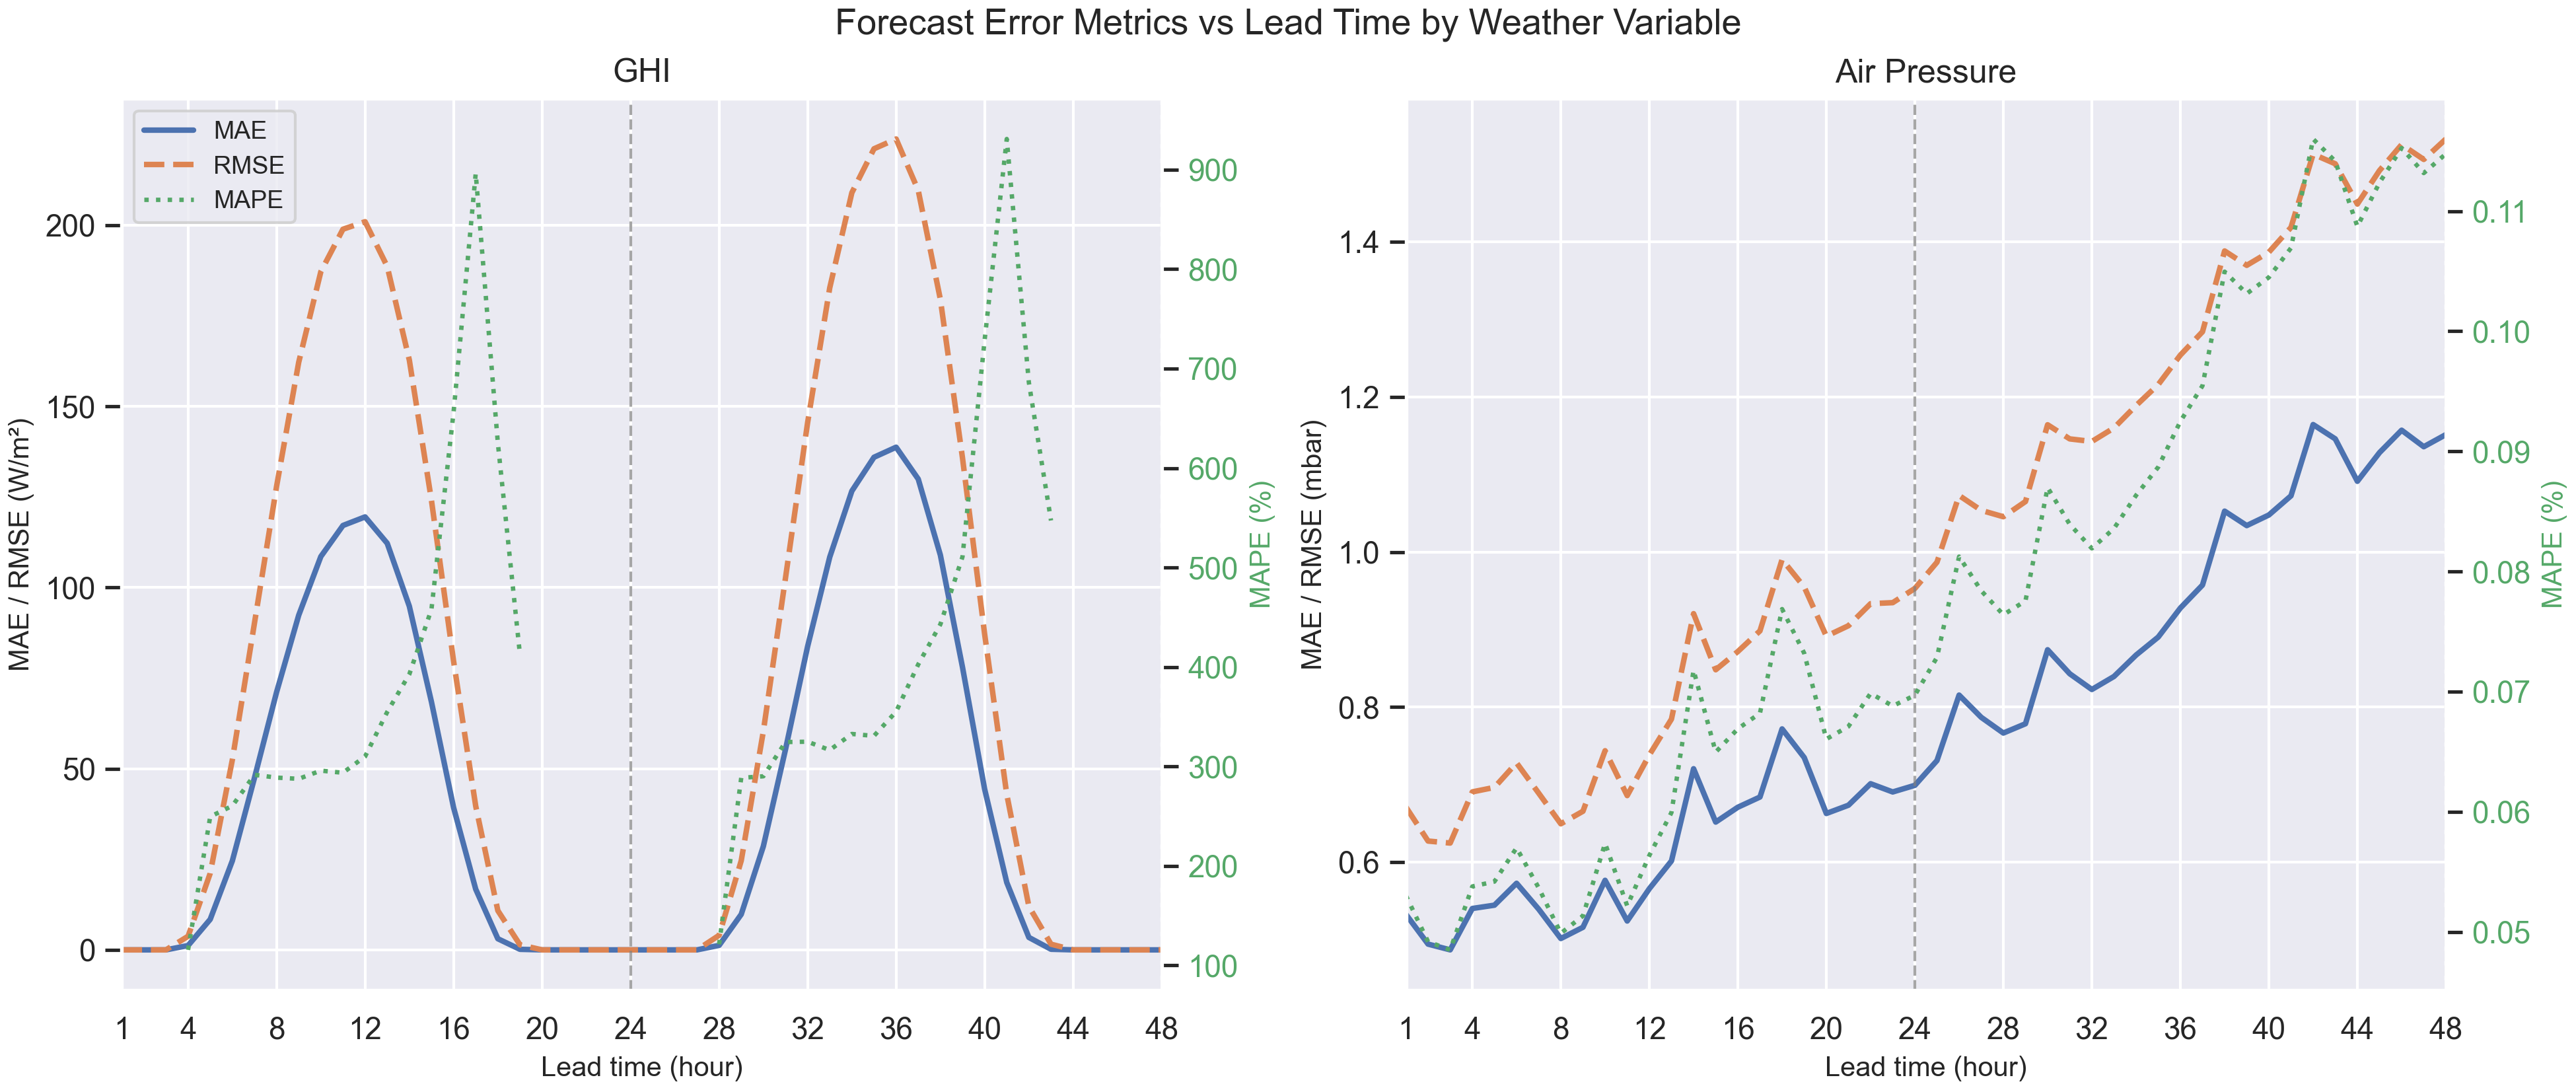
\includegraphics[width=\textwidth]{figures/Q2/embed/error_by_lead_time_ghi_pressure copy.png}
  \caption{Forecast error metrics versus lead time, by variable. MAE (solid) and RMSE (dashed)
  are on the left axis in native units; MAPE (dotted) is on the right twin axis in percent.
  MAE and RMSE generally grow with lead time and show twin peaks near lead~12 and~36---the
  diurnal signature created by the fixed \texttt{06z} init (those leads fall near solar noon).
  RMSE $\ge$ MAE throughout, with the gap widening slightly, indicating that larger errors
  become relatively more frequent further out. GHI rises from and returns to $\approx 0$ twice
  (it is $\approx 0$ at night); its MAPE is unstable, so MAPE is only interpretable for pressure
  and relative humidity.}
  \label{fig:leadtime}
\end{figure}

The key observations are: (i) MAE and RMSE rise with lead time and (ii) exhibit two diurnal peaks at
roughly leads 12--16 and 36--40; (iii) RMSE exceeds MAE throughout and the gap widens slightly with lead,
implying that forecast stability drops as the horizon grows; and (iv) MAPE is only meaningful
for pressure and relative humidity---for the other variables the small or zero denominators
inflate it beyond use. The exception to (i) is GHI because irradiance drops to 0 at night, and the exception to (ii) is air pressure, as its plot shows several oscillations instead of two diurnal peaks.

\subsection{Error growth rate}

We define the \emph{error-growth rate} as the change in the error between
consecutive lead hours, $\Delta\text{Error}/\text{hr}$. Figure~\ref{fig:growthcurves} shows the
fleet-mean growth curve per variable, and Figure~\ref{fig:growthdist} shows the box plot distributions of the error growths for each lead time.

\begin{figure}[H]
  \centering
  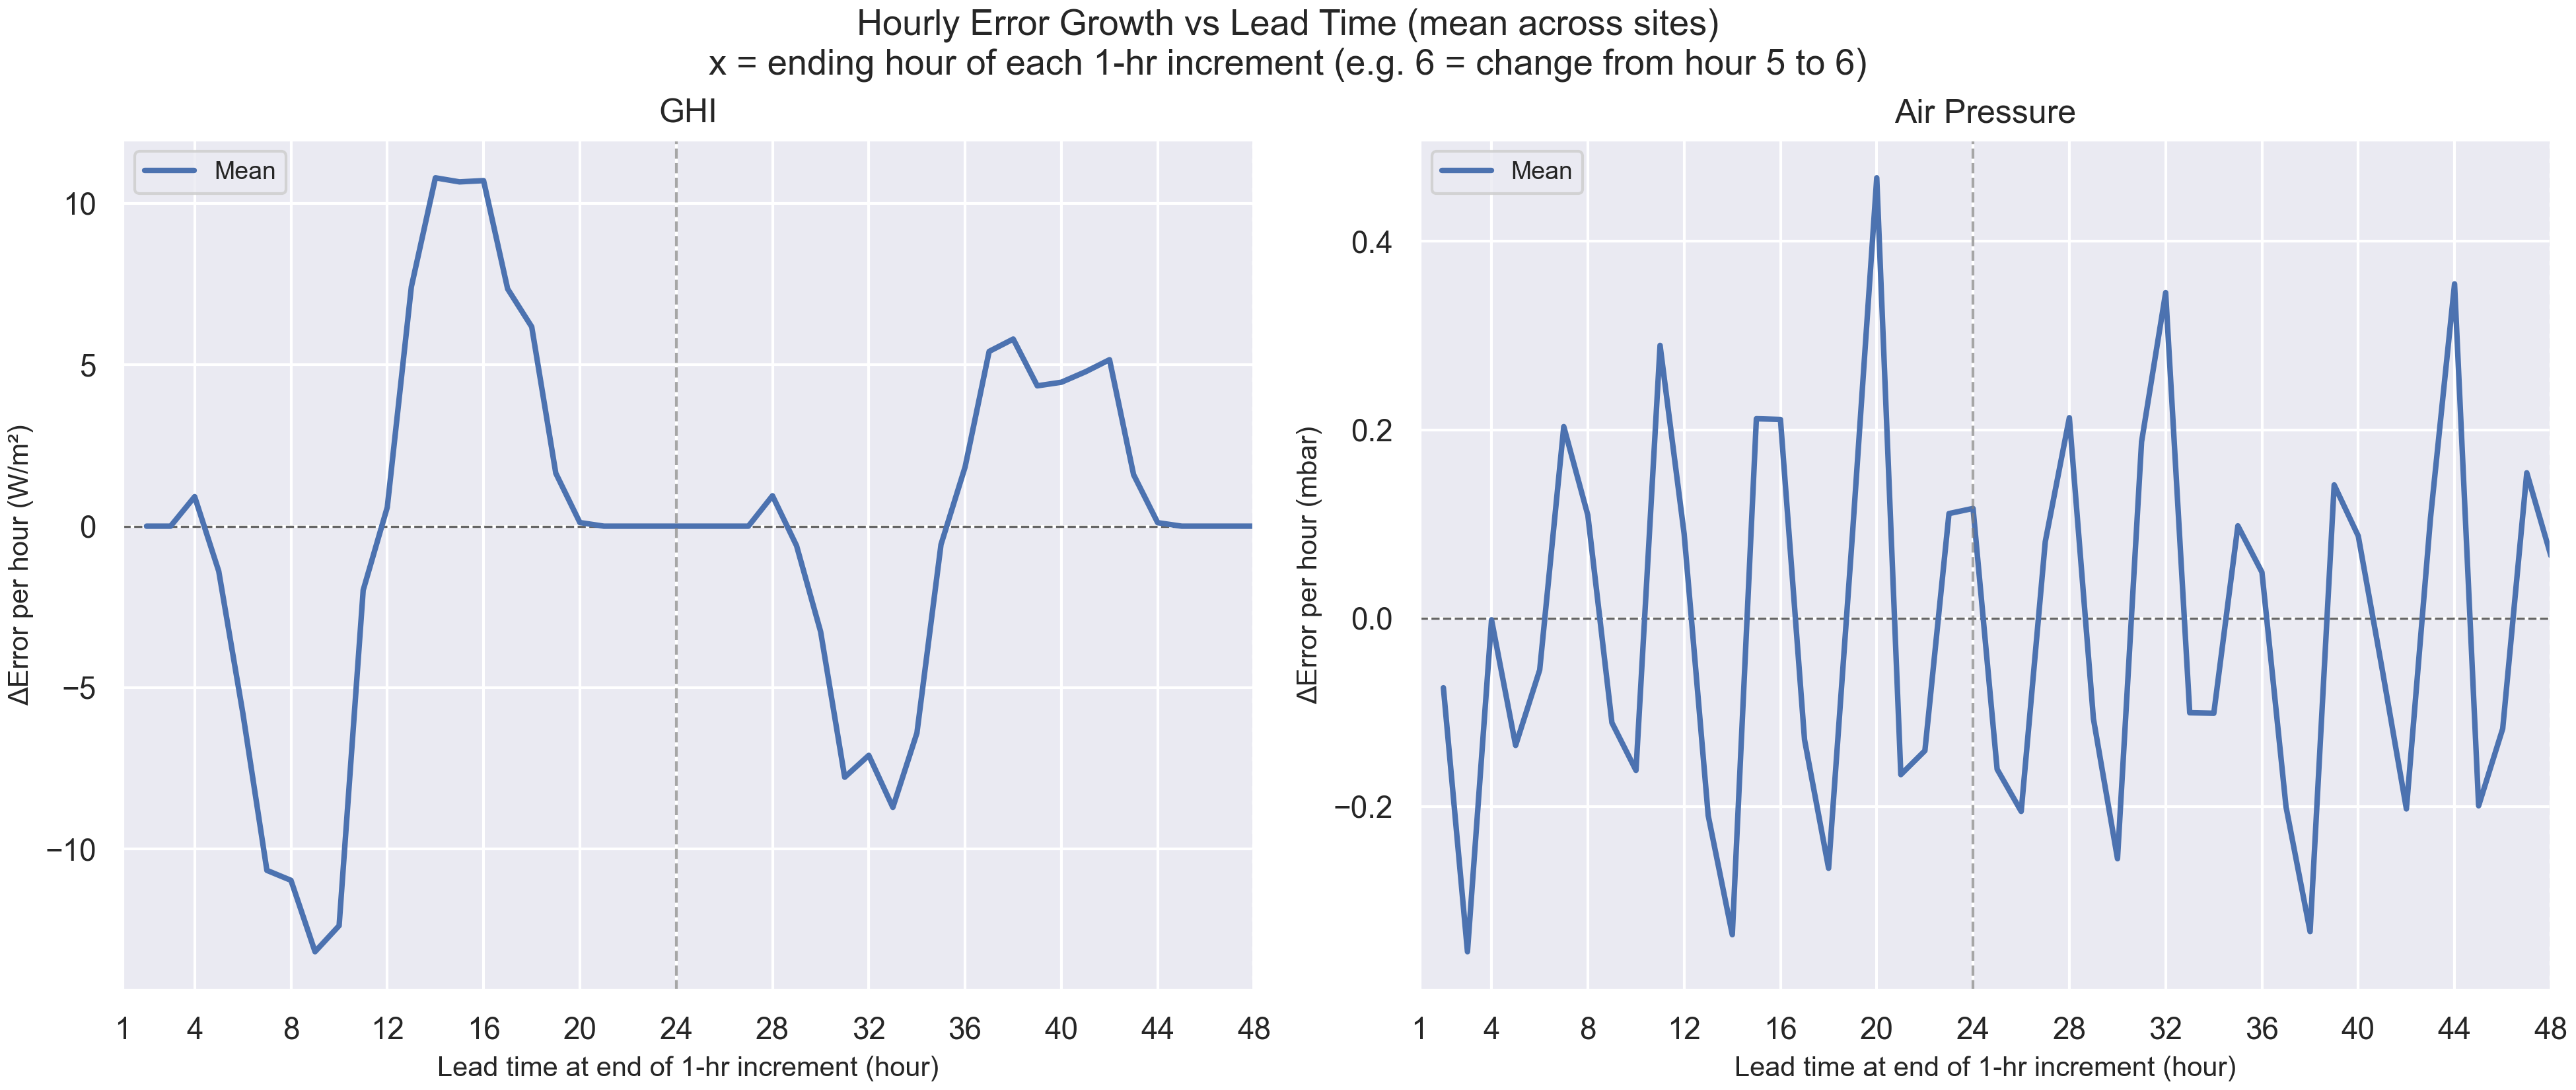
\includegraphics[width=\textwidth]{figures/Q2/embed/error_growth_curves_ghi_pressure copy.png}
  \caption{Fleet-mean hourly error-growth rate ($\Delta\text{Error}/\text{hr}$) versus lead time.
  GHI traces a clear diurnal sinusoid (least volatile near sunrise/sunset); the other variables
  hover around zero with no obvious trend, and pressure is the noisiest. Curves oscillating
  around zero---rather than staying positive---indicate that bias does not drift monotonically
  with lead time.}
  \label{fig:growthcurves}
\end{figure}

\begin{figure}[H]
  \centering
  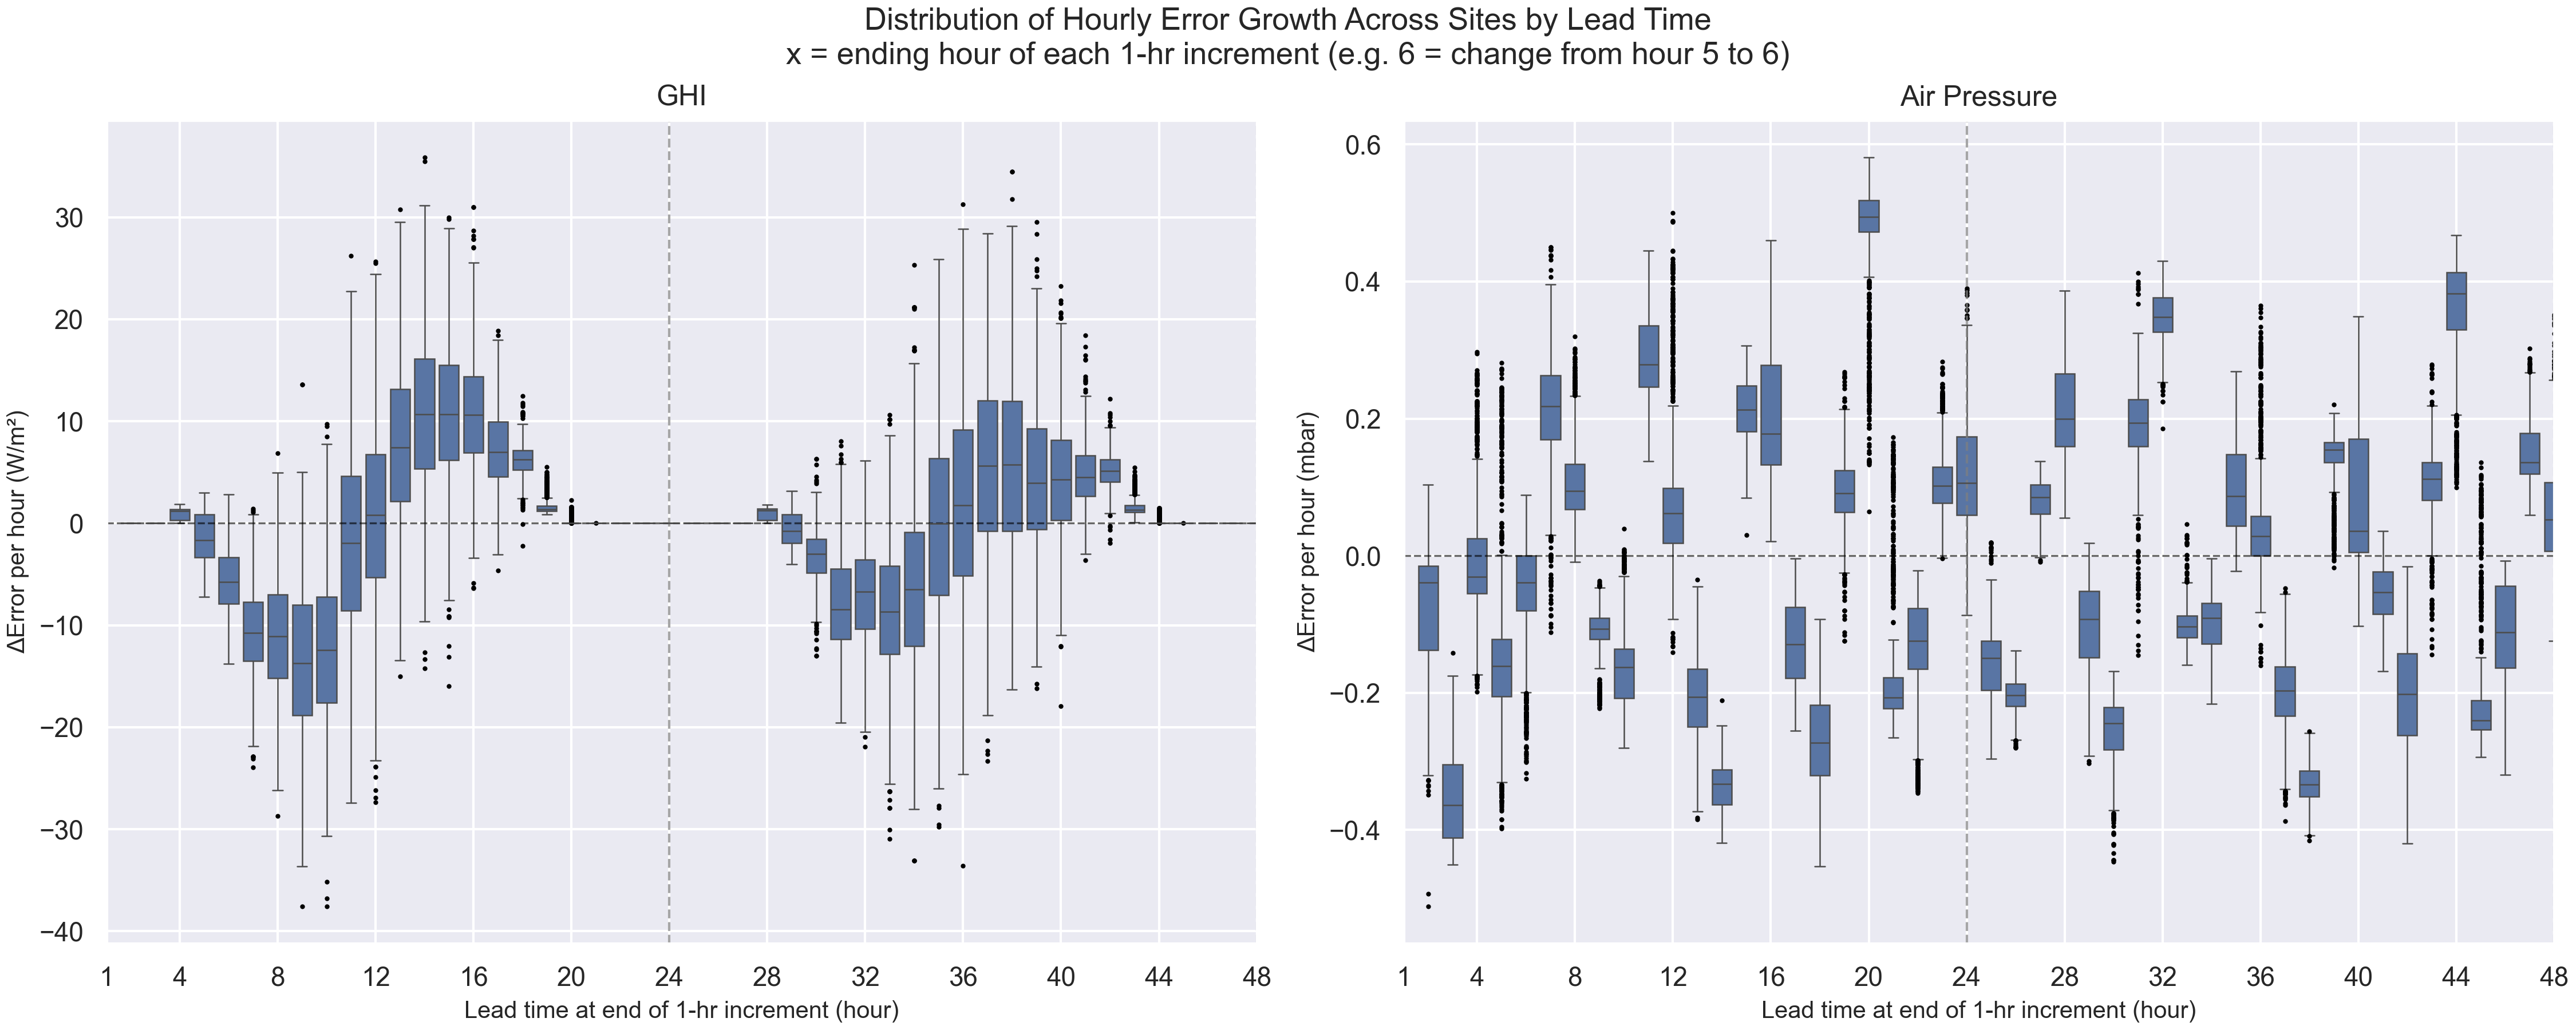
\includegraphics[width=\textwidth]{figures/Q2/embed/error_growth_distributions_ghi_pressure copy.png}
  \caption{Distribution of the hourly error-growth rate ($\Delta\text{Error}/\text{hr}$) across
  all \num{896} sites at each lead time, one boxplot per lead hour and one panel per variable.
  GHI shows the diurnal sinusoid in its box centres with visibly larger spread during the day;
  the other variables stay centred near zero with roughly constant spread across lead time,
  indicating that error-growth volatility does not systematically increase further out. Pressure
  has the widest boxes (most volatile across sites).}
  \label{fig:growthdist}
\end{figure}

As shown by these plots, GHI has the most prominent sinusoidal pattern with a 24-hr cycle, but a few other weather variables hint at this as well, such as relative humidity. Furthermore, it seems that for all variables the error growth rate is centered at 0 across all lead times. These observations warranted statistical tests to evaluate their significance.

\subsection{Statistical testing}

We ran two tests to assess the significance of these two findings. Multiple-comparison control uses
the Benjamini--Hochberg FDR procedure throughout.

\begin{description}
  \item[Test 1 --- Harmonic / diurnal cycle.] We fit the error growth to a harmonic regression,
        $\text{growth}(h) = A\sin(2\pi h/24) + B\cos(2\pi h/24) + C$, and used permutation tests
        on the amplitude. After FDR correction, the amplitudes for \textbf{GHI, RH, U10, and
        wind direction} are statistically significant, supporting a genuine 24-hour cycle in
        those variables.
  \item[Test 2 --- Bias drift.] A Wilcoxon test for a systematic bias shift across the horizon
        found \emph{no} variable with a statistically significant drift---error growth does not
        lean consistently positive or negative.
\end{description}

\begin{figure}[H]
  \centering
  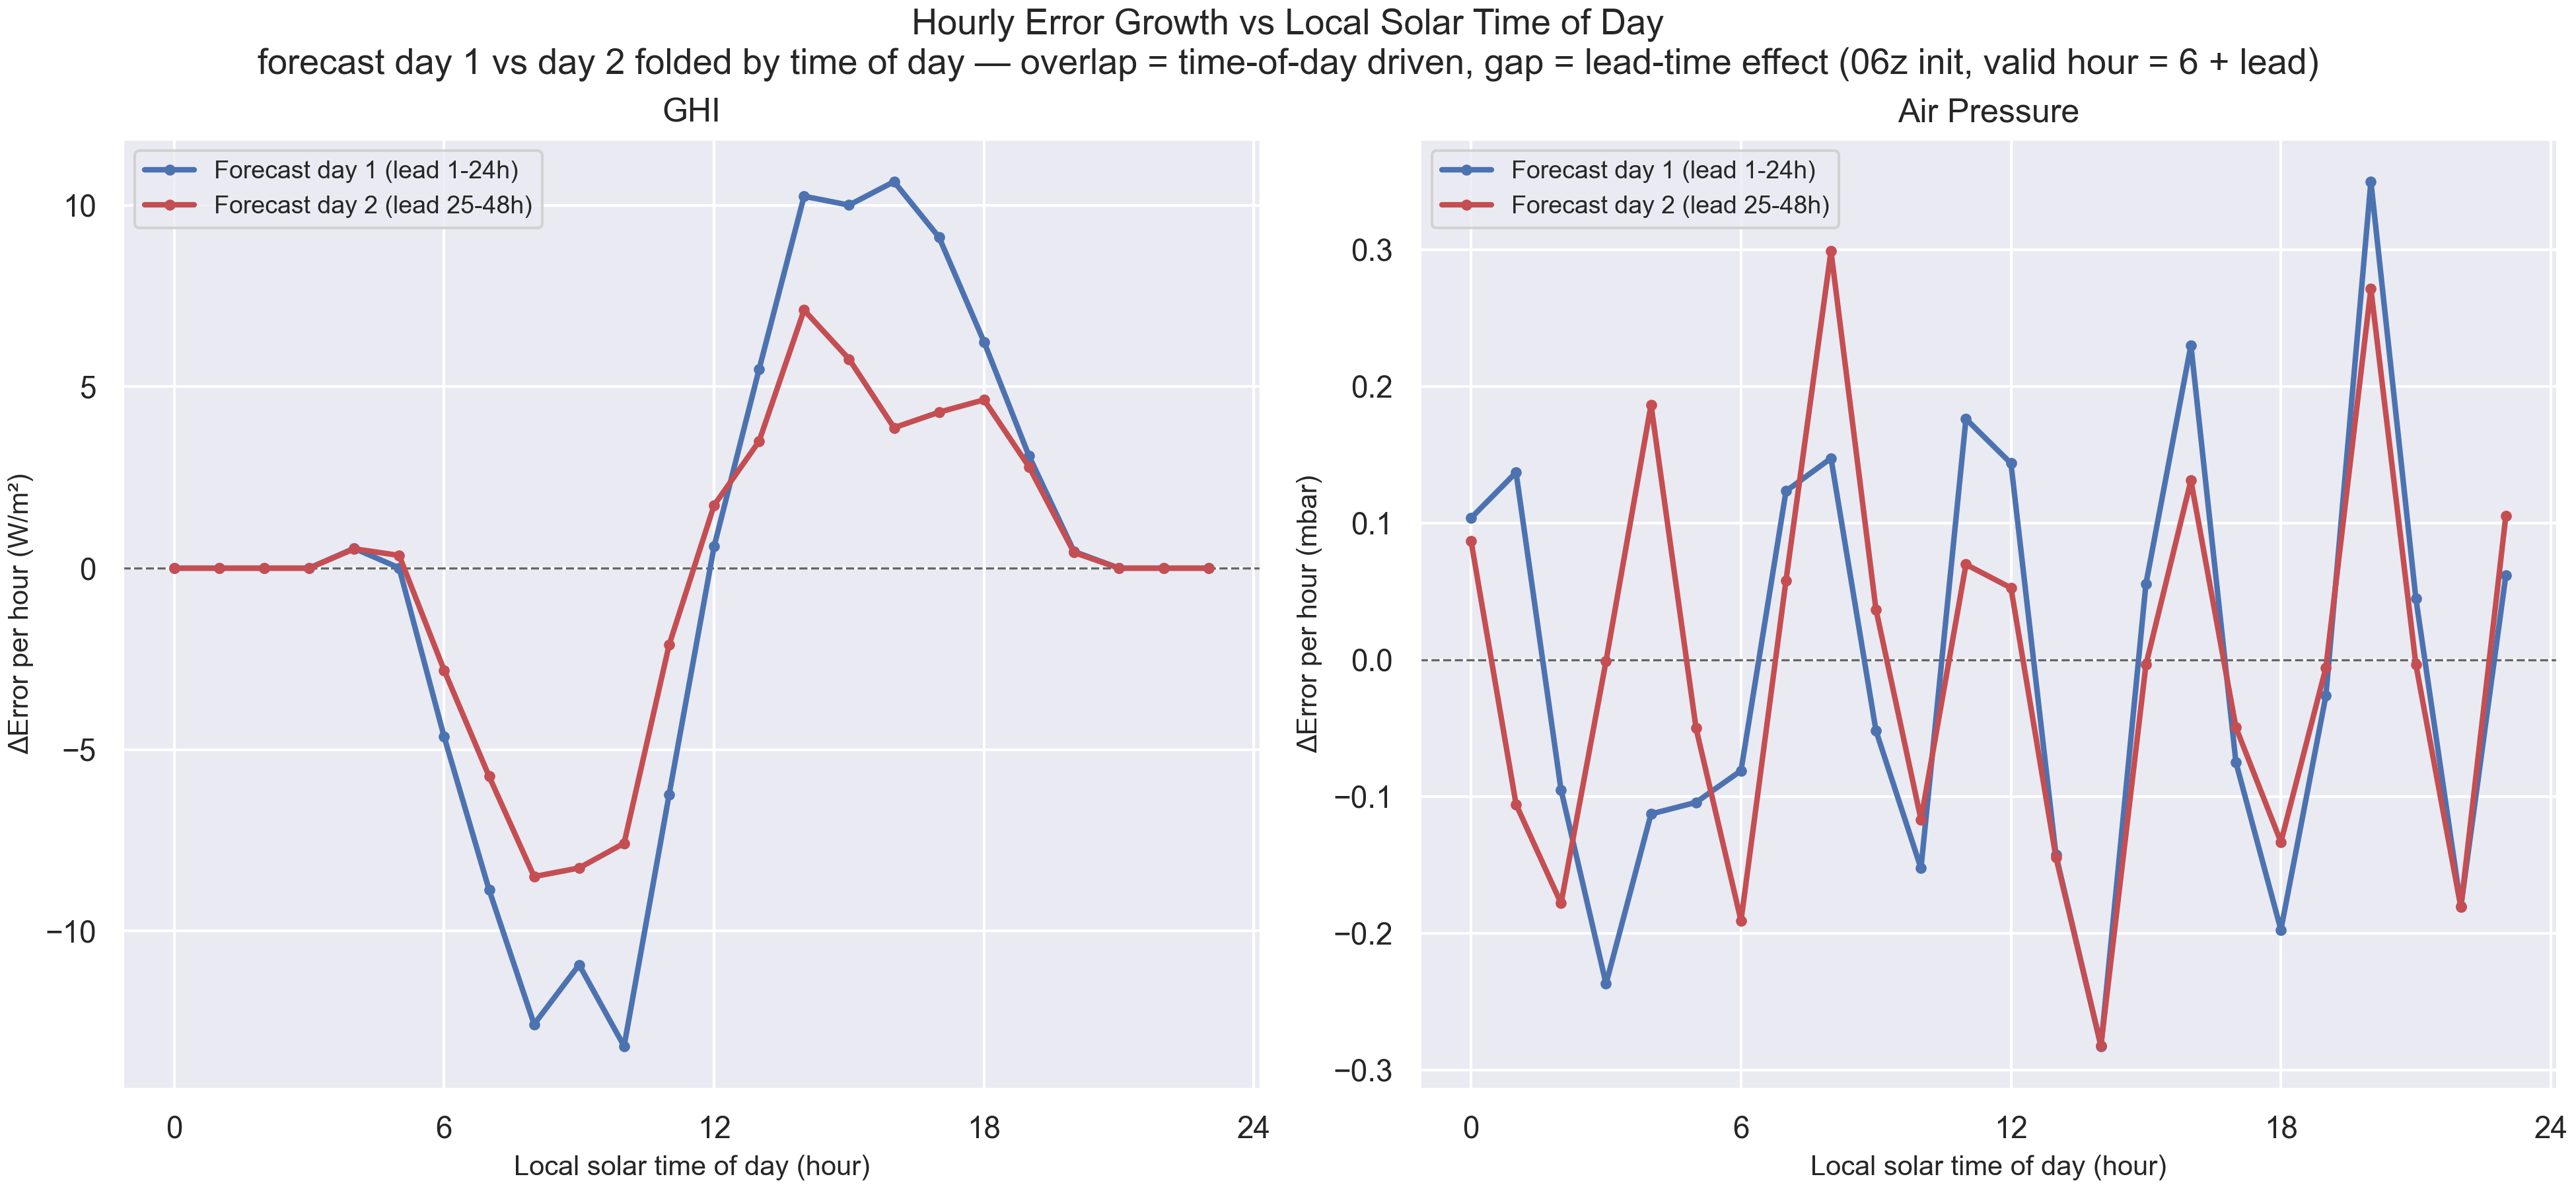
\includegraphics[width=\textwidth]{figures/Q2/embed/error_growth_tod_ghi_pressure copy.png}
  \caption{Hourly error growth folded onto local solar time of day, with forecast day~1
  (leads 1--24~h) and day~2 (leads 25--48~h) overlaid. Because lead $h$ and lead $h{+}24$ land
  at the same time of day, overlapping lines indicate a purely time-of-day signal, while a
  vertical gap would indicate a genuine lead-time effect. The two days track closely for most
  variables, confirming the growth pattern is time-of-day driven.}
  \label{fig:tod}
\end{figure}

\subsection{Implications}

Forecast errors are largest at lead times of 12--16 and 36--40 hours, so day-ahead grid
scheduling at those horizons carries the most uncertainty. Since MAE and RMSE gradually rise and have a widening gap across lead times and RMSE weighs larger errors more, larger errors are more frequent for longer lead times. This implies taht forecast stability drops as lead time goes up. Because error growth centers on zero
for every variable, scheduling is not expected to systematically over- or under-commit. Most
usefully, the significant 24-hour cycle in GHI, RH, U10, and wind direction is \emph{correctable}:
one can model the bias as a function of time of day with harmonic regression and subtract it from
the forecast.

% ======================================================================
\newpage
\section{Q3 --- Forecast Error vs. Predicted Hour}

\textbf{Research question:}

\begin{quote}
Is the forecast error dependent on the predicted hour? How does this relationship vary by weather variable, PJM zone, season, and year?
\end{quote}

\subsection{Data and Method}

Forecast errors were computed for the December 30 and December 31 forecast cycles and evaluated across the 48 forecast hours. To test whether forecast error depends on predicted hour, the Kruskal--Wallis test was applied across forecast-hour groups.

Because the dataset is very large, statistical significance alone is not the most useful measure of practical importance. Therefore, epsilon-squared effect size is emphasized more heavily than p-values when interpreting the strength of forecast-hour dependence.

\subsection{Descriptive Error Patterns by Forecast Hour and Weather Variable}

The per-variable forecast-hour line plots show how mean forecast error changes over the 48-hour horizon. The normalized all-variable heatmap provides a compact comparison across weather variables.

Overall, forecast-hour dependence is not uniform across variables. GHI and pressure show clearer forecast-hour structure, while wind direction and wind-component errors show weaker forecast-hour structure.


\subsection{Statistical Evidence for Forecast-Hour Dependence}

The all-site Kruskal--Wallis epsilon-squared summary provides the main statistical evidence for whether forecast error depends on forecast hour.

The strongest forecast-hour dependence appears for GHI and pressure, with mean epsilon-squared values of 0.0524 and 0.0506, respectively. Relative humidity and temperature show moderate forecast-hour dependence, with mean epsilon-squared values of 0.0308 and 0.0284. Wind speed has a mean epsilon-squared value of 0.0149, U wind, V wind, and wind direction have the weakest dependence with the values of 0.0087, 0.0085, and 0.0044 respectively.

These results suggest that forecast hour matters most for GHI and pressure errors, moderately for relative humidity and temperature errors, and weakly for wind-variable errors.

\begin{figure}[H]
    \centering
    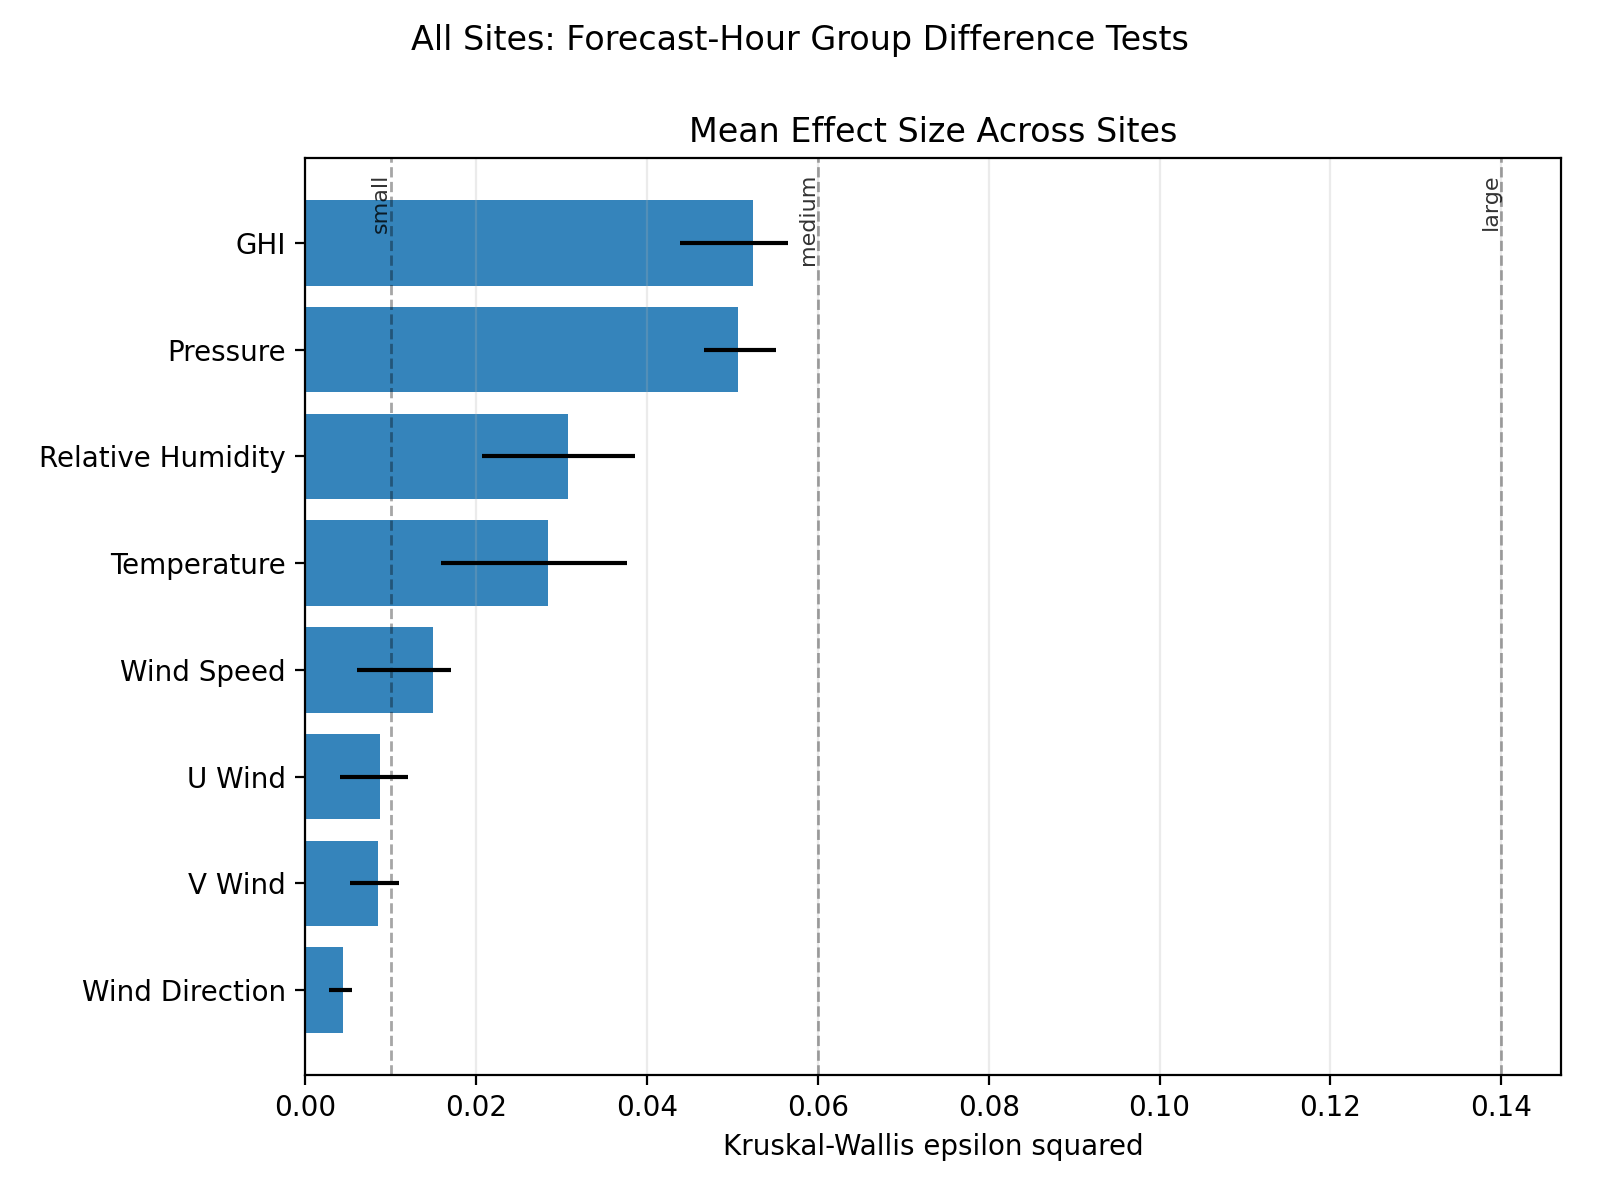
\includegraphics[width=0.60\textwidth]{figures/Q3/section_5_figures/5_2_statistical_test/kruskal_forecast_hour_epsilon_summary_allsites.png}
    \caption{Mean epsilon-squared effect size from Kruskal--Wallis tests across forecast-hour groups.}
    \label{fig:kruskal_forecast_hour_summary}
\end{figure}

\subsection{Variation by Season}

The forecast-hour-by-season heatmap and summary figure show whether the forecast-hour relationship changes by season.

Pooled across seasons, pressure, GHI, relative humidity, and temperature have the largest forecast-hour effect sizes. Summer is especially important for relative humidity, temperature, and pressure. Fall also shows strong pressure forecast-hour dependence. Wind variables remain weaker than radiation, pressure, temperature, and humidity, although summer increases wind-speed and wind-component effects somewhat.

\begin{figure}[H]
    \centering
    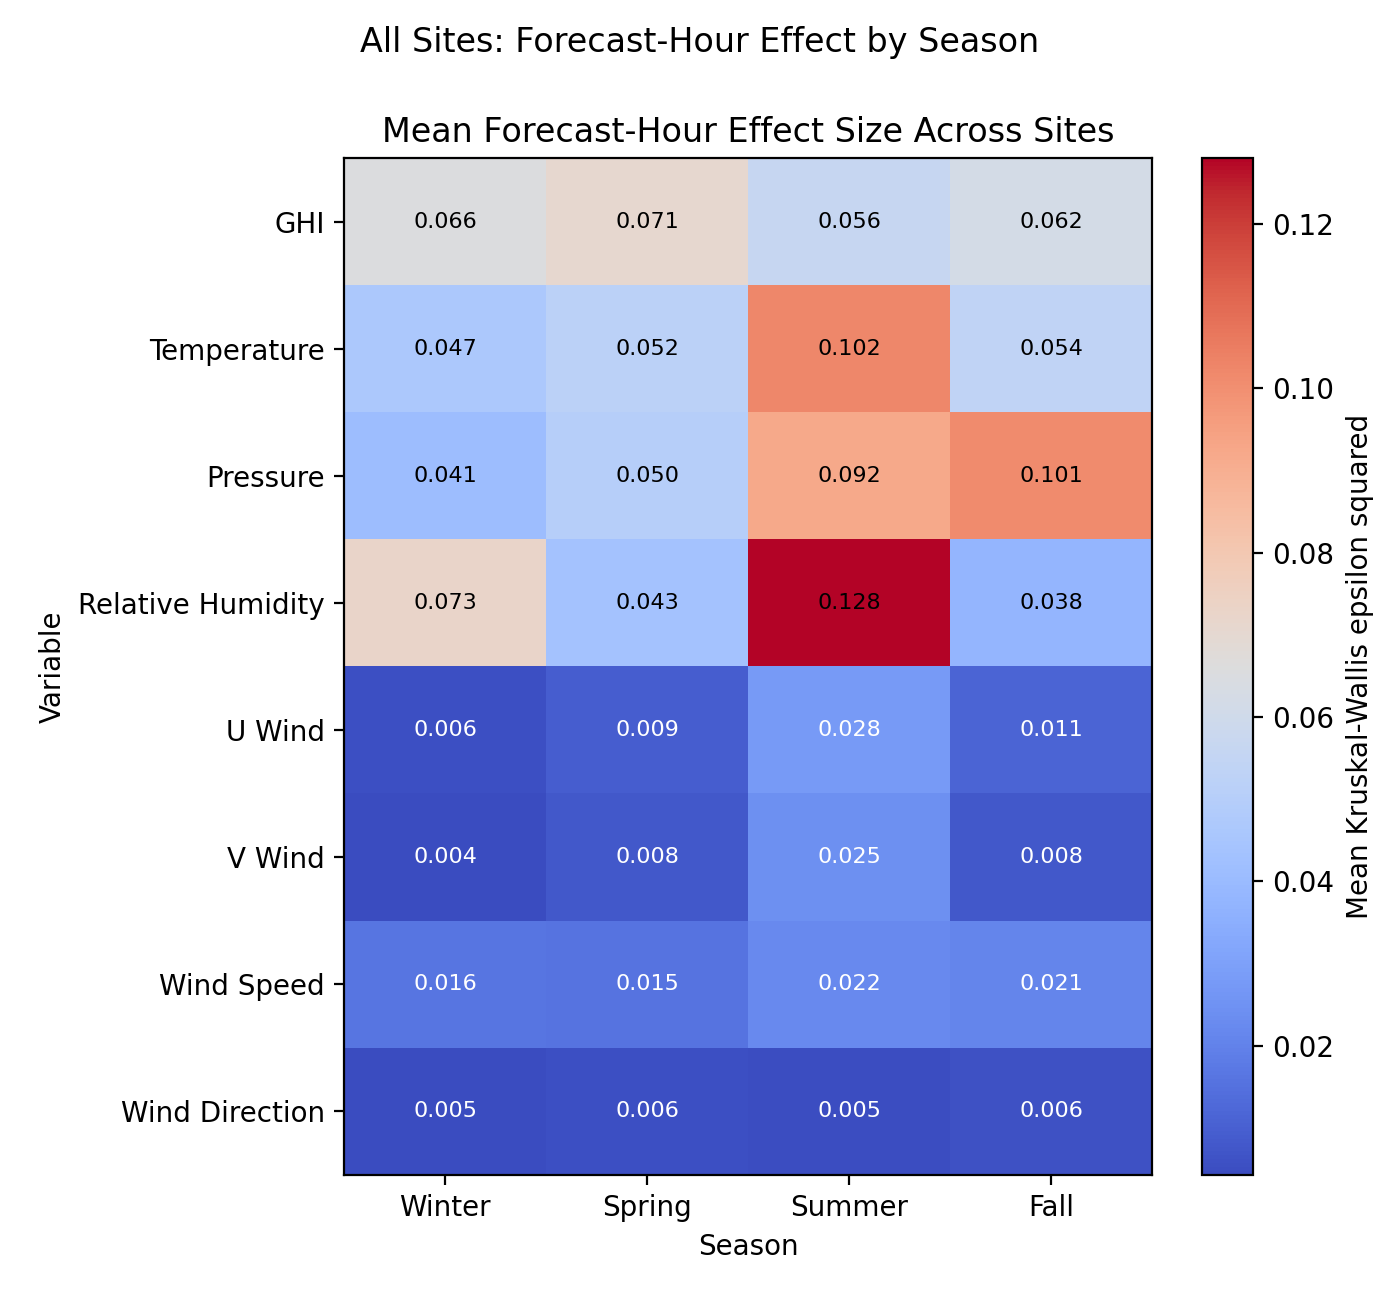
\includegraphics[width=0.60\textwidth]{figures/Q3/section_5_figures/5_3_season/kruskal_forecast_hour_by_season_epsilon_heatmap_allsites.png}
    \caption{Forecast-hour dependence by season, measured using epsilon-squared effect size.}
    \label{fig:forecast_hour_season_heatmap}
\end{figure}

\begin{figure}[H]
    \centering
    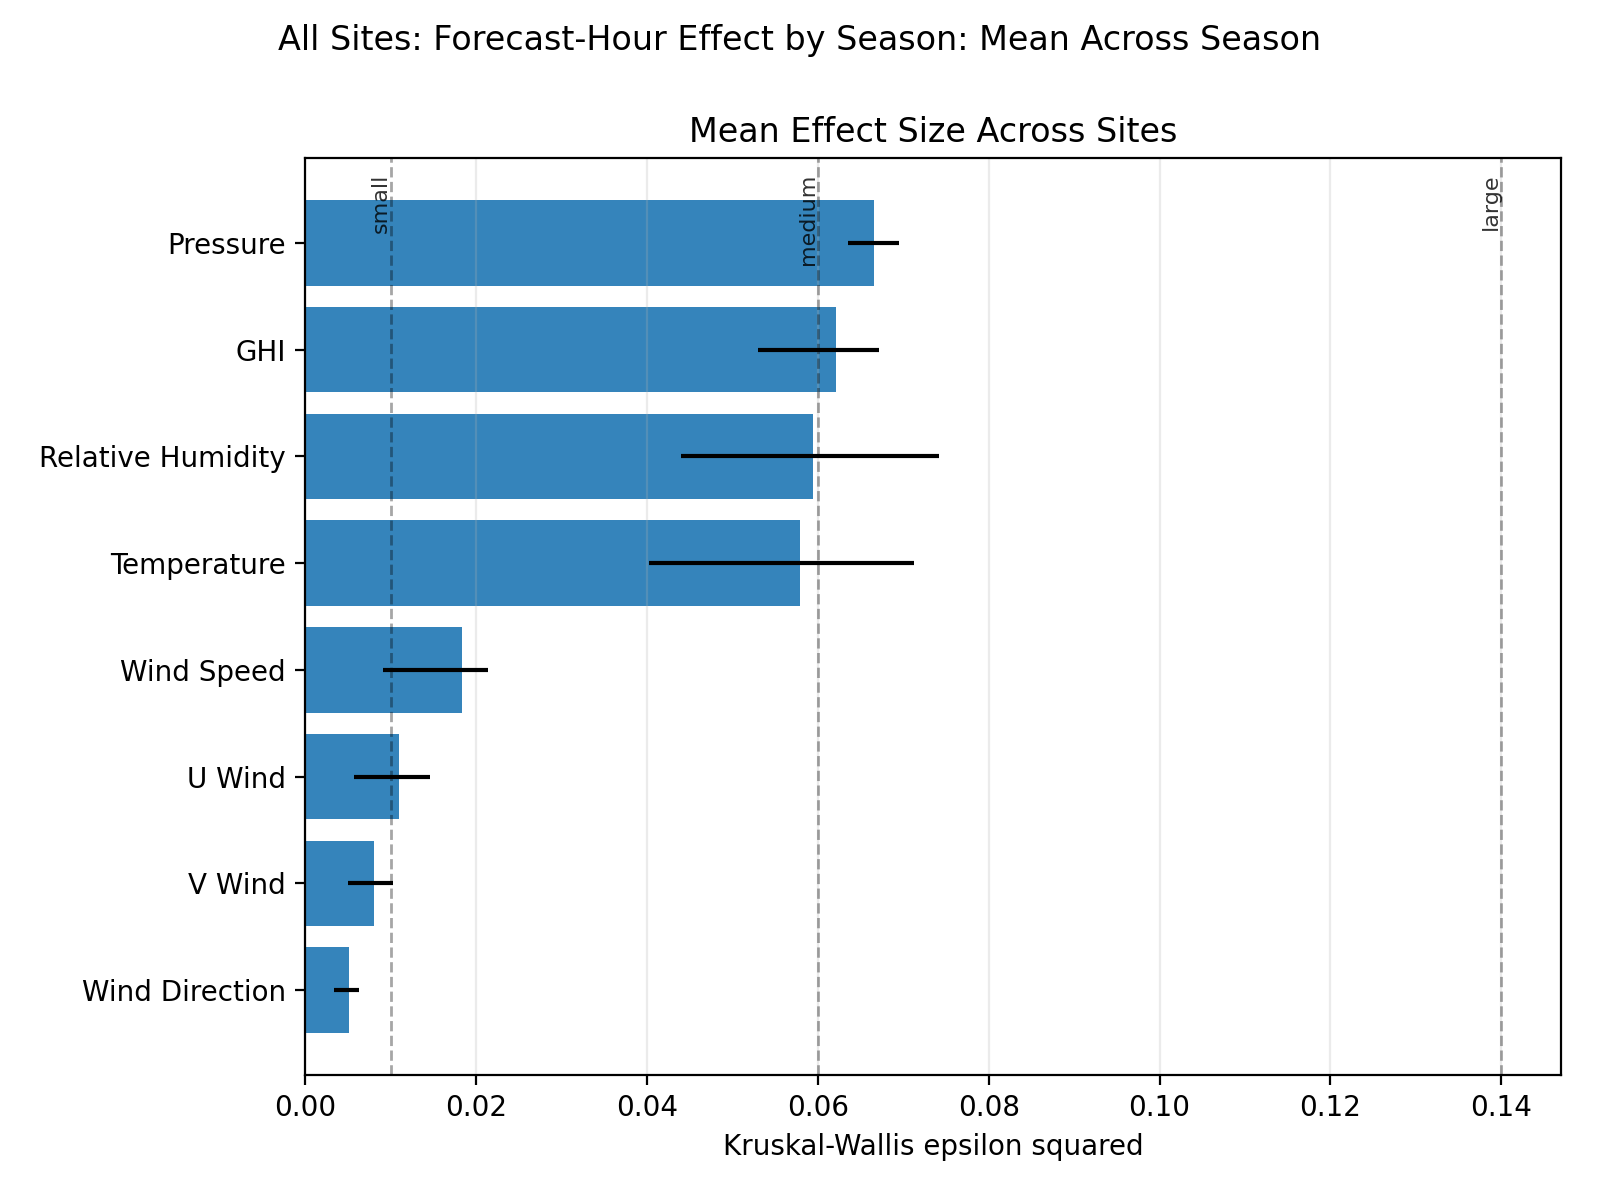
\includegraphics[width=0.60\textwidth]{figures/Q3/section_5_figures/5_3_season/kruskal_forecast_hour_by_season_epsilon_summary_allsites.png}
    \caption{Seasonal summary of forecast-hour dependence across weather variables.}
    \label{fig:forecast_hour_season_summary}
\end{figure}

\subsection{Variation by Year}

The forecast-hour-by-year heatmap and summary figure show whether forecast-hour dependence changes across years.

The year-stratified pattern is broadly stable. Pressure and GHI remain the strongest forecast-hour-dependent variables in 2022, 2023, and 2024. Temperature and relative humidity are consistently moderate. Wind speed, U wind, V wind, and wind direction remain comparatively weak.

\begin{figure}[H]
    \centering
    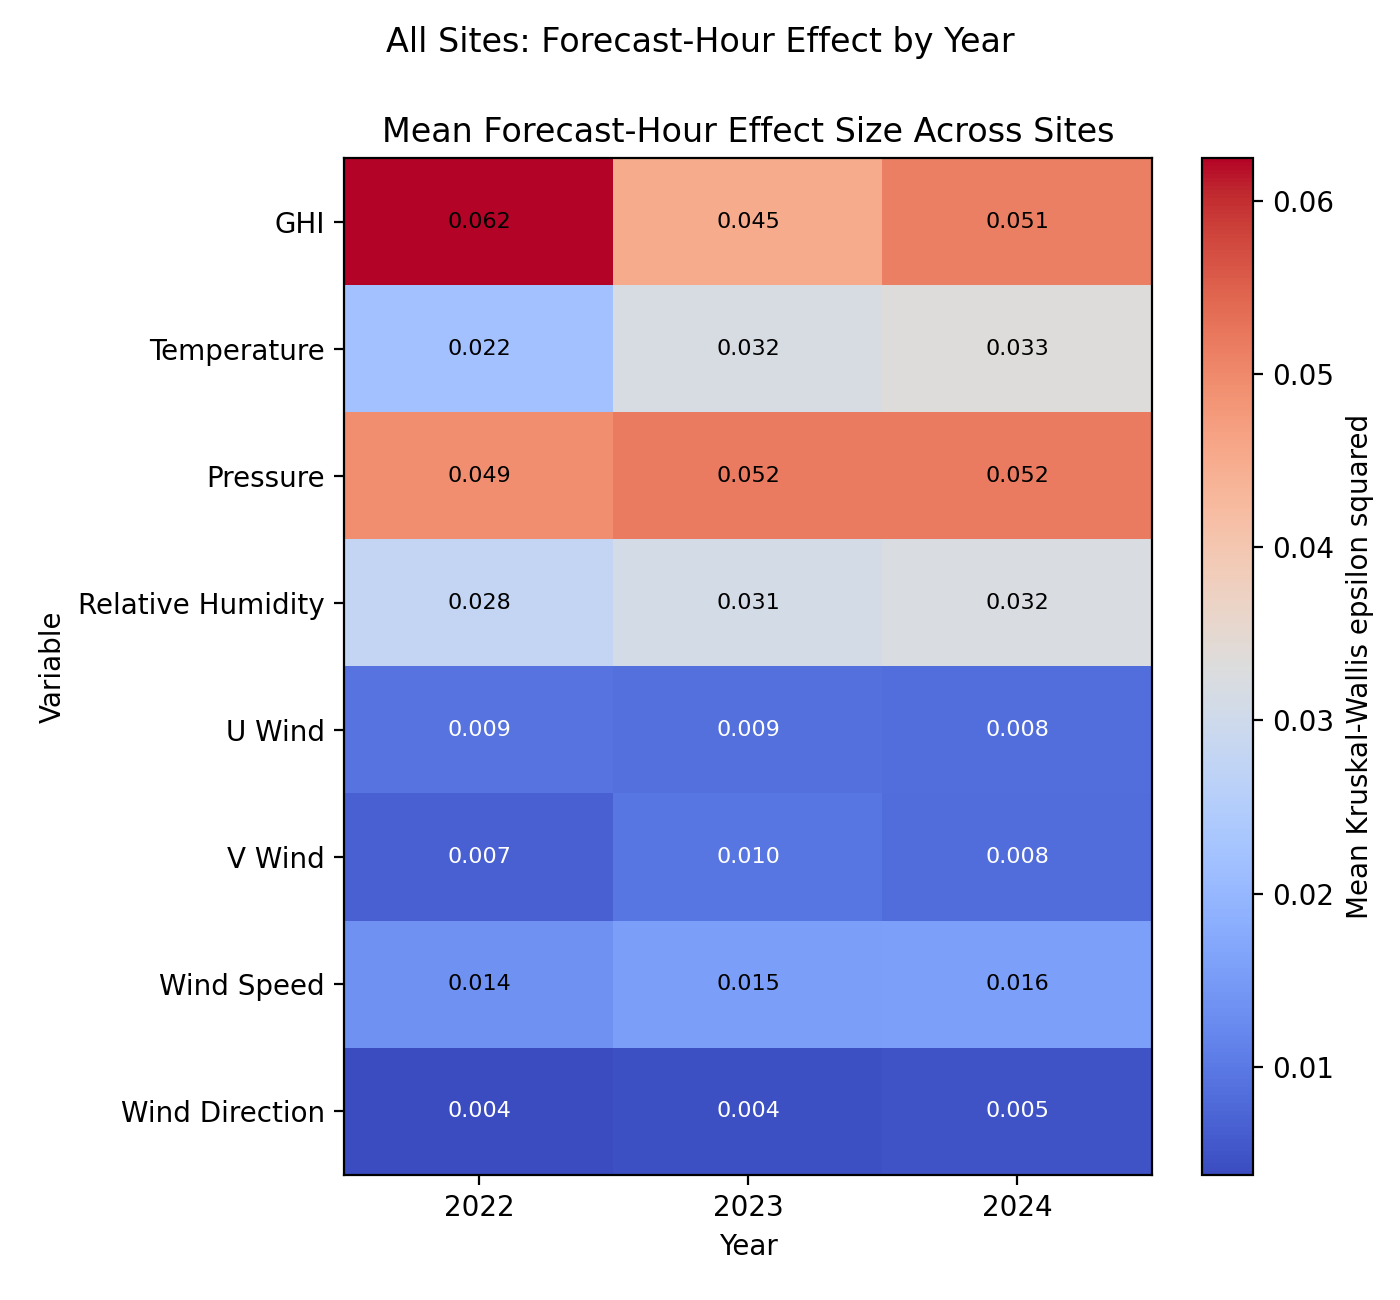
\includegraphics[width=0.60\textwidth]{figures/Q3/section_5_figures/5_4_year/kruskal_forecast_hour_by_year_epsilon_heatmap_allsites.png}
    \caption{Forecast-hour dependence by year, measured using epsilon-squared effect size.}
    \label{fig:forecast_hour_year_heatmap}
\end{figure}

\begin{figure}[H]
    \centering
    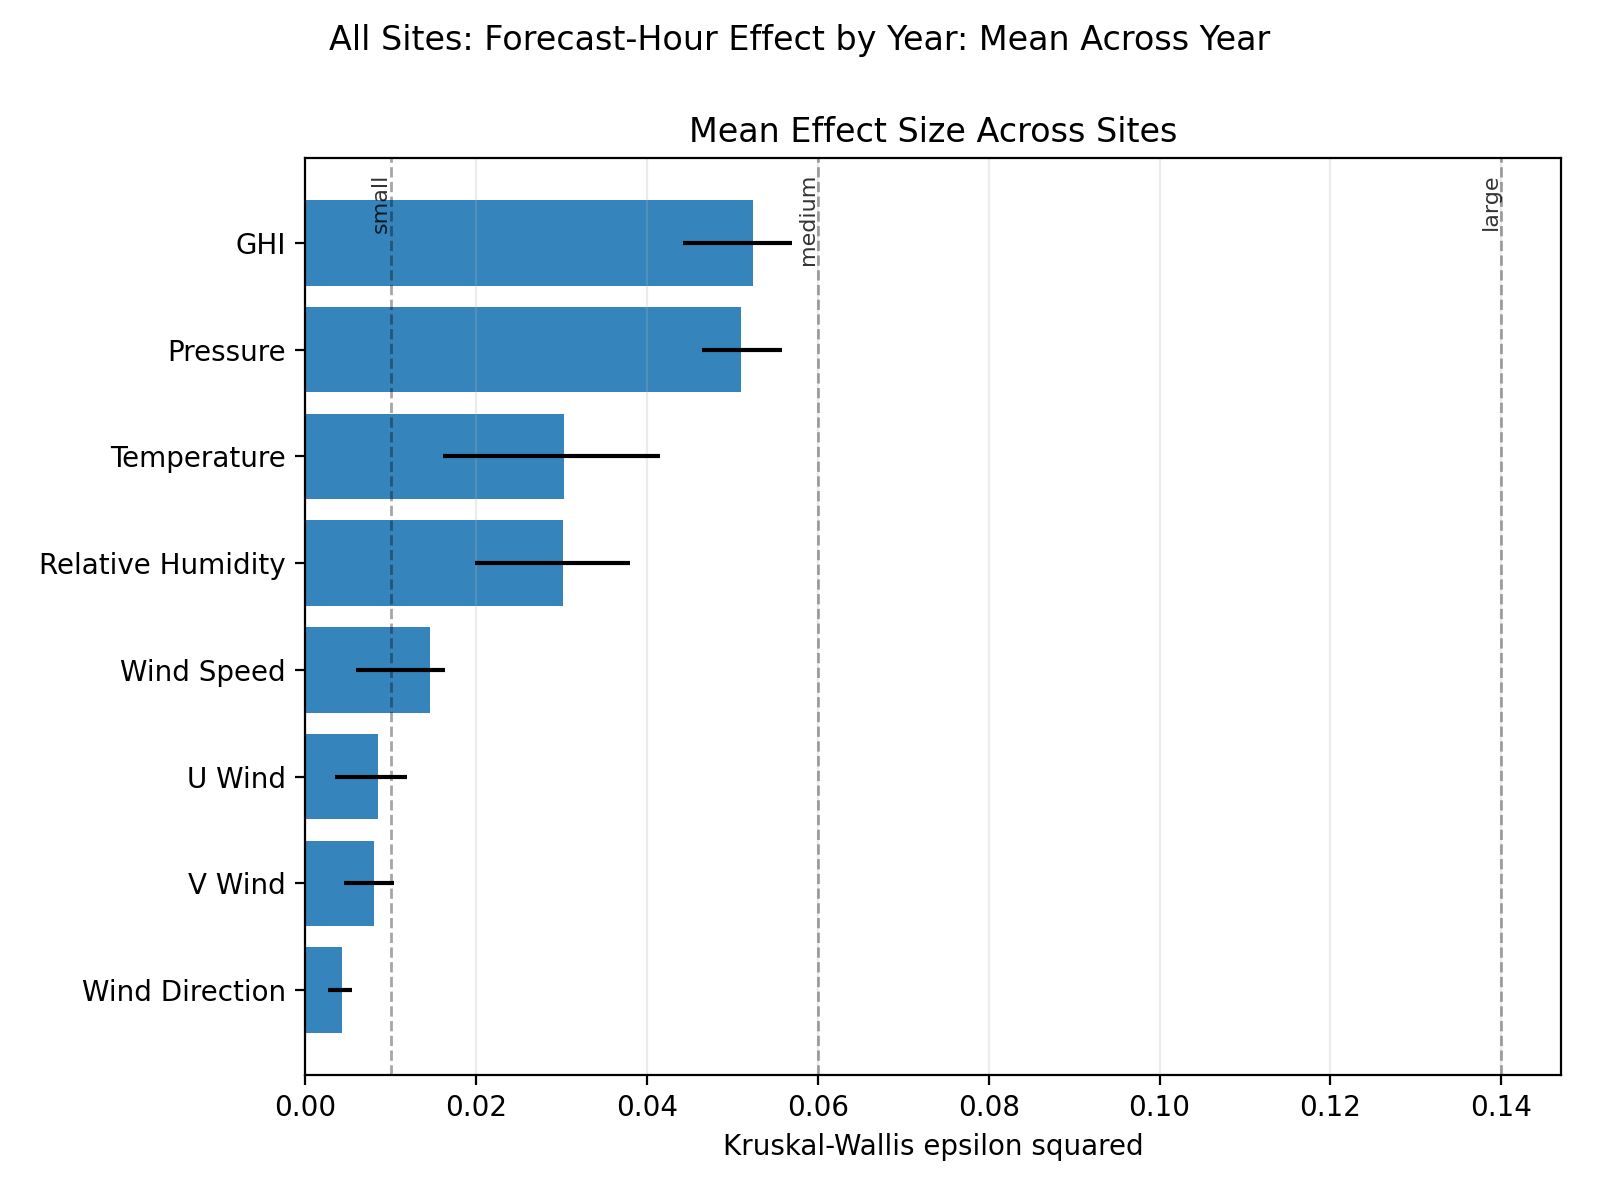
\includegraphics[width=0.60\textwidth]{figures/Q3/section_5_figures/5_4_year/kruskal_forecast_hour_by_year_epsilon_summary_allsites.png}
    \caption{Yearly summary of forecast-hour dependence across weather variables.}
    \label{fig:forecast_hour_year_summary}
\end{figure}

\subsection{Conclusion}

Forecast error is dependent on forecast hour, but the strength of that dependence varies substantially by weather variable. The clearest forecast-hour effects occur for GHI and pressure, followed by relative humidity and temperature. Wind variables show weaker dependence on forecast hour.

Seasonal stratification reveals stronger forecast-hour effects in specific seasons, especially summer for temperature and relative humidity and fall or summer for pressure. Year-to-year differences are smaller than variable and seasonal differences. PJM-zone variation still requires a dedicated zone-stratified analysis.


% ======================================================================

\section{Q4 and Q5 — Autocorrelation Structure of Forecast Errors}

\subsection{Average ACF and PACF Behavior}

We created box plots of the averaged autocorrelation function (ACF) and the partial autocorrelation function (PACF) for the raw forecast errors of all eight variables. The plots are based on lead time for each forecast run across all 896 sites and all three years. Each sequence represents a 48-hour forecast run at one site, and the lags in the graphs represent the differences between lead times.

The main findings are as follows.
\begin{itemize}
    \item From the ACF graphs, GHI errors remain related for about 3 lags, temperature for about 6 lags, pressure for about 9 lags, and RH for about 6 lags.
    \item In the PACF plots, the first lag is clearly dominant for all variables. The strongest PACF lag-1 value was for temperature, with an average value of about 0.88, while the weakest was for wind direction, with an average value of about 0.27.
    \item U10, V10, wind speed, and wind direction seem to have similar behavior. They remain related for around 5 hours, then the autocorrelation centers around zero for the remaining lags.
\end{itemize}

\begin{figure}[H]
    \centering
    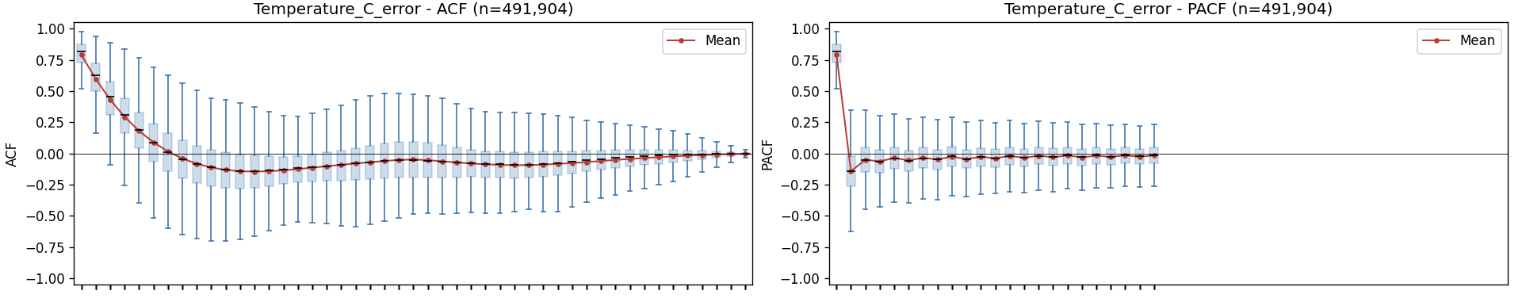
\includegraphics[width=\textwidth]{figures/Q4 & Q5/Temperature_ACF_PACF.png}
    \caption{ACF vs. lag on the left and PACF vs. lag on the right for temperature. The ACF values drop quickly from lag 1 onward. By around lags 8--15, most variables are close to zero or slightly negative.}
    \label{fig:Temperature_ACF_PACF}
\end{figure}

\begin{figure}[H]
    \centering
    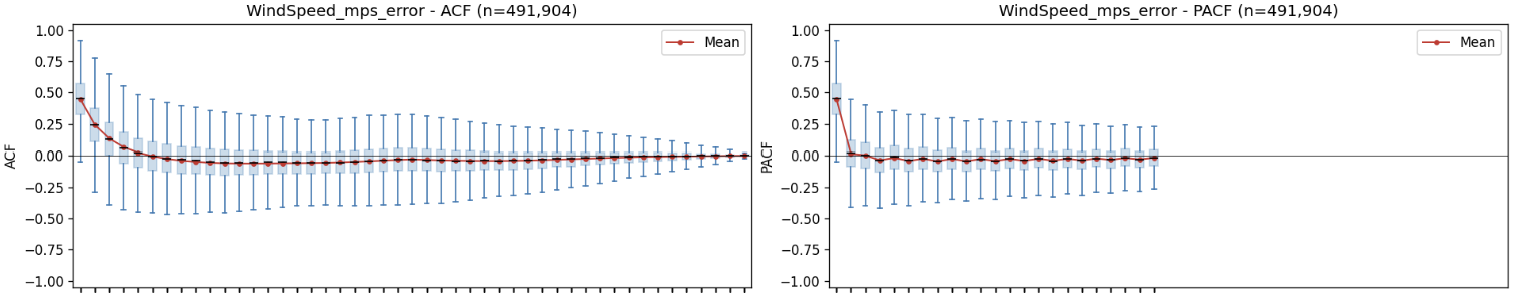
\includegraphics[width=\textwidth]{figures/Q4 & Q5/WindSpeed_ACF_PACF.png}
    \caption{ACF vs. lag on the left and PACF vs. lag on the right for wind speed.}
    \label{fig:WindSpeed_ACF_PACF}
\end{figure}

\subsection{Differences by Season, Year, Zone, and Time of Day}

We calculated the average ACF and PACF values for sequences grouped by four seasons, three years, four times of day, and nine zones. After that, we ran the Kruskal-Wallis test to see whether the average ACF and PACF curves differed by season, year, time of day, and zone, as shown in Figure~\ref{fig:kw_heatmap}.

The main findings are as follows.
\begin{itemize}
    \item The strongest difference appears in pressure ACF by season with $p = 0.12$, but this is still not below the usual 0.05 significance level.
    \item Wind variables show some weaker differences by season, such as U10 and V10 with $p = 0.19$, and wind speed with $p = 0.20$.
\end{itemize}

\begin{figure}[H]
    \centering
    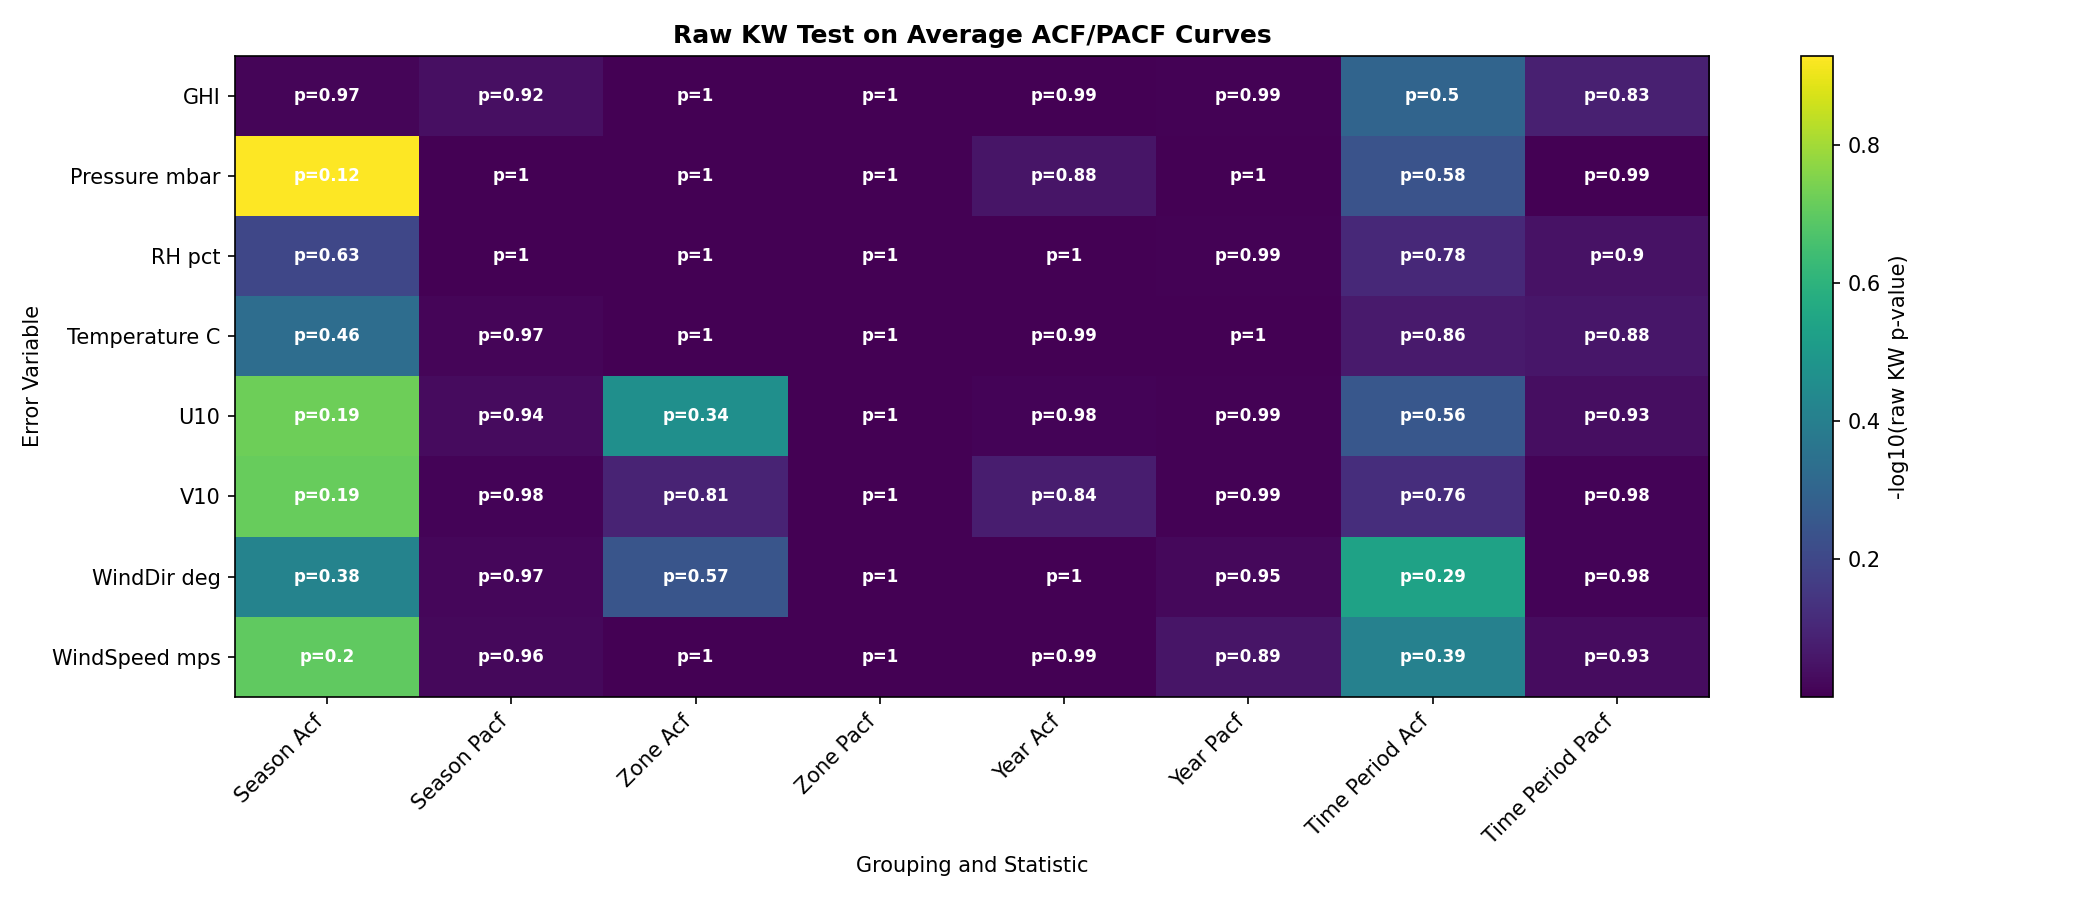
\includegraphics[width=\textwidth]{figures/Q4 & Q5/acf_pacf_average_curve_raw_kw_heatmap.png}
    \caption{The rows list the error variables, and the columns show the grouping being compared: season, zone, year, or time of day, separately for ACF and PACF. Each cell shows the raw Kruskal-Wallis p-value, where smaller p-values suggest stronger differences between the average curves.}
    \label{fig:kw_heatmap}
\end{figure}

\subsection{Implications}

Forecast errors show short-term persistence. However, this persistence weakens as the gap between forecast hours increases. If the model has an error at one forecast hour, nearby forecast hours tend to have similar errors. Most of the direct autocorrelation structure appears at the immediately previous forecast hour. Moreover, there is no strong statistical evidence that the correlations differ meaningfully across years and zones. Season and time of day show slightly more variation than zone and year, but the differences are still not statistically significant.

\section{Q6 — Cross-Variable Forecast Error Correlations}


\textbf{Research question:}

\begin{quote}
How are forecast errors correlated across weather variables, and which variables tend to have related forecast-error behavior?
\end{quote}

\subsection{Data and Method}

Forecast errors from the December 30 and December 31 forecast cycles were combined across all available sites. Before computing correlations, duplicate observations were grouped by site ID and valid time, and the mean error was used for each site-time pair. This produced 23,505,664 aligned site-time observations across 896 sites.

For each pair of weather variables, the Pearson correlation coefficient was computed between their forecast-error time series. Only rows where both error values were finite were included. The resulting Pearson value measures the linear relationship between two forecast errors:

\[
r = \frac{\mathrm{cov}(X,Y)}{\sigma_X \sigma_Y}.
\]

A positive value means that the two forecast errors tend to increase or decrease together. A negative value means that one error tends to increase when the other decreases. A value near zero means that there is little linear relationship between the two error series.

\subsection{Pairwise Error Correlation Heatmap}

The pairwise correlation heatmap summarizes the Pearson correlation values across all weather-variable error pairs. Blue cells represent negative correlations, red cells represent positive correlations, and lighter cells represent correlations closer to zero.

\begin{figure}[H]
    \centering
    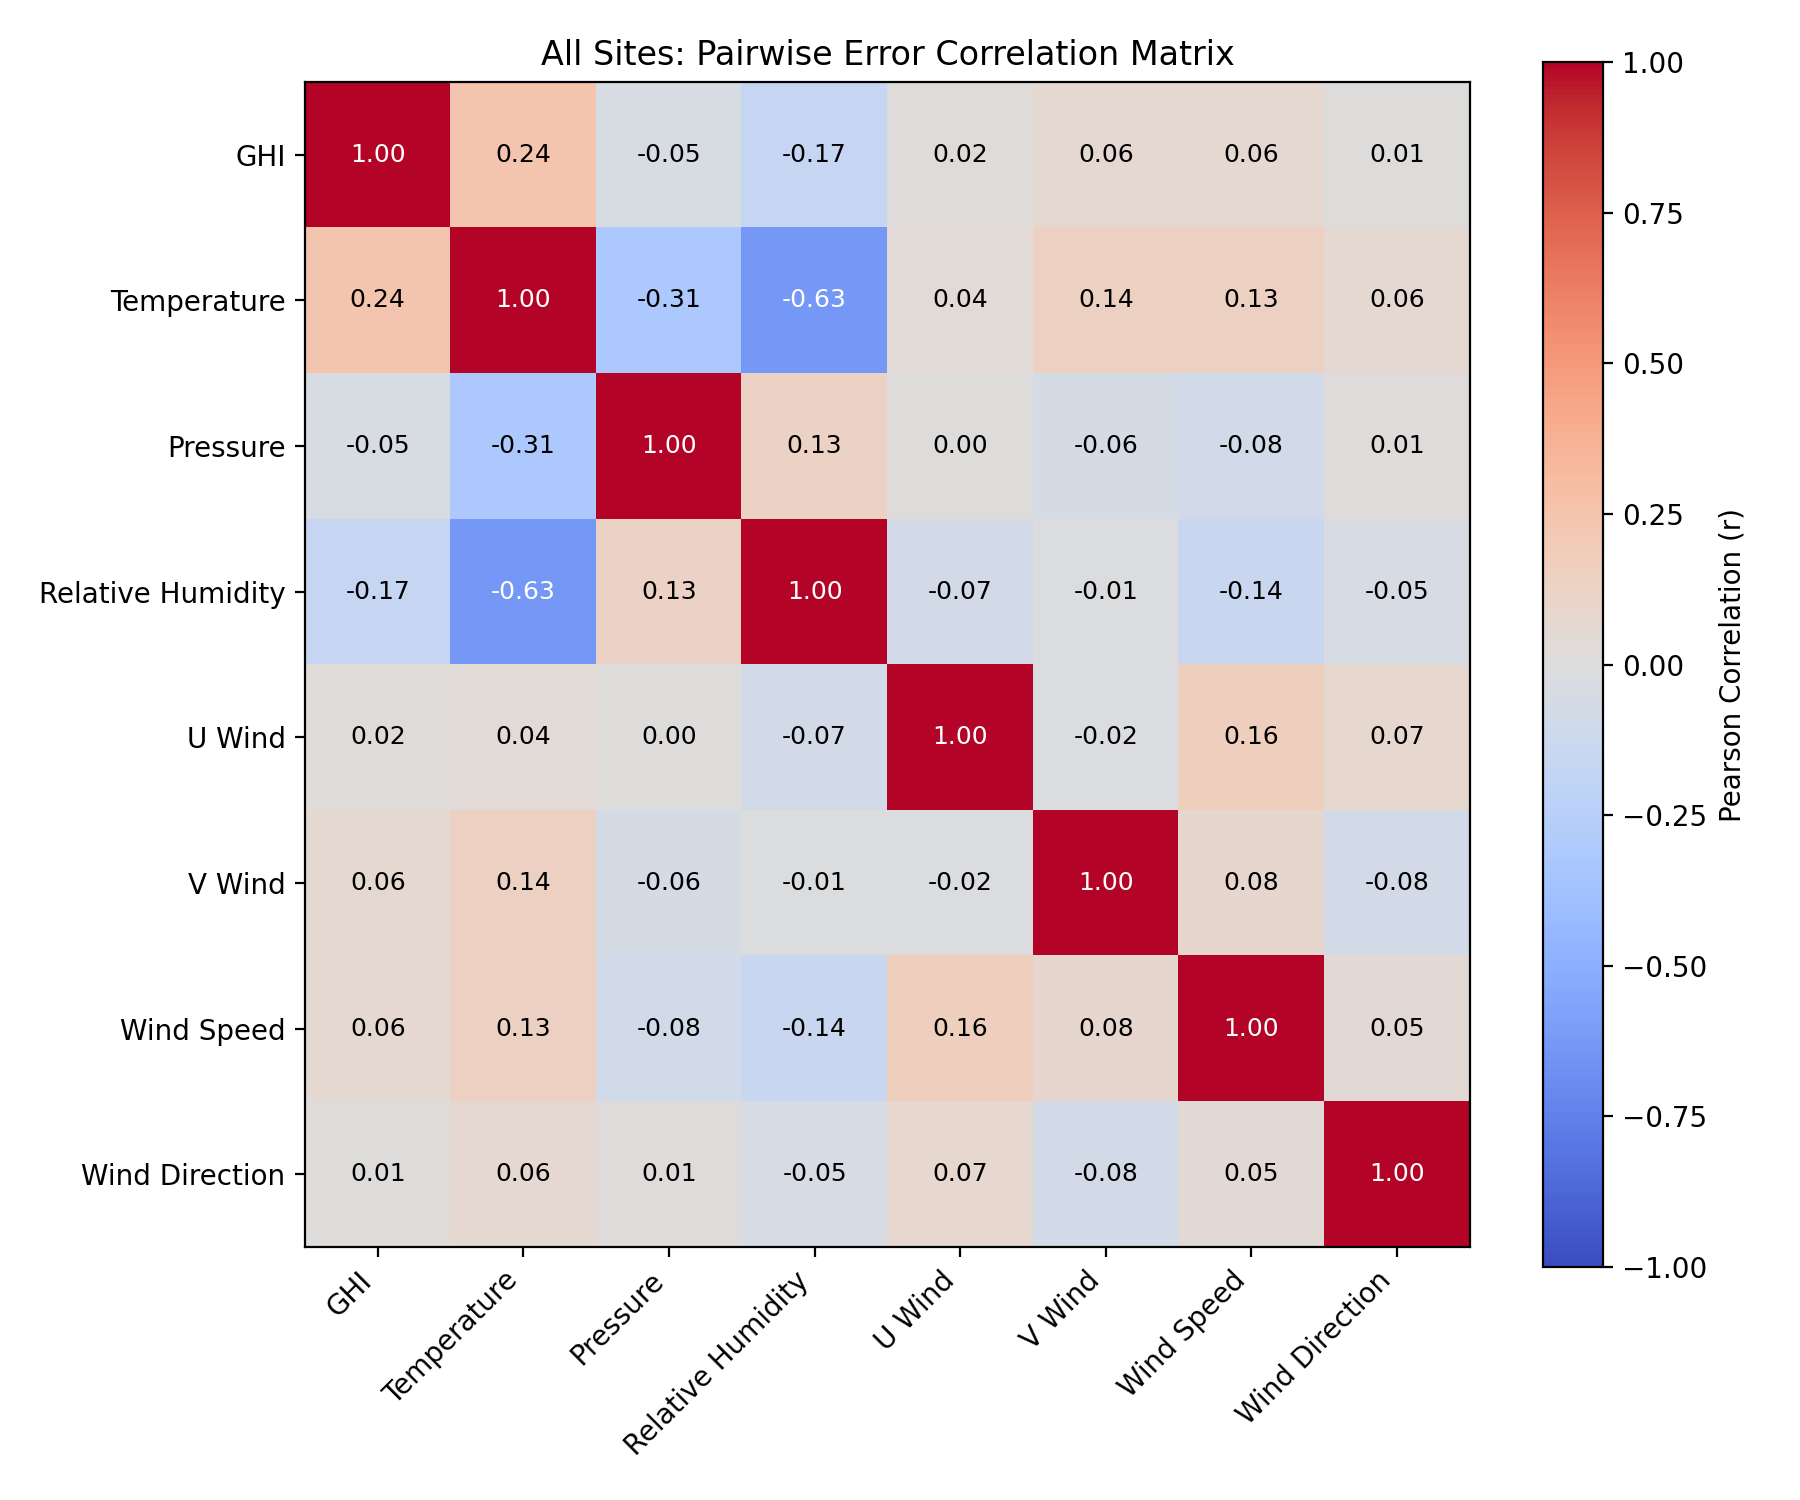
\includegraphics[width=0.65\textwidth]{figures/Q6/allsites_pairwise_error_correlation_matrix.png}
    \caption{Pairwise Pearson correlations between forecast-error variables across all sites and valid times.}
    \label{fig:q6_pairwise_error_correlation}
\end{figure}

\subsection{Main Correlation Patterns}

The strongest cross-variable relationship is between temperature error and relative humidity error, with a Pearson correlation of approximately $r=-0.626$. This negative relationship means that positive temperature forecast errors tend to occur with negative relative-humidity forecast errors, and vice versa. This is physically reasonable because temperature and relative humidity are closely connected through atmospheric moisture capacity.

Temperature error also has a moderate negative relationship with pressure error, with $r=-0.313$, and a weaker positive relationship with GHI error, with $r=0.238$. These values suggest that temperature-error behavior is more connected to other thermodynamic and radiation-related errors than to wind errors.

Most wind-variable relationships are comparatively weak. U wind and V wind have a correlation close to zero, $r=-0.023$, and their relationships with wind speed are also weak: U wind vs. wind speed has $r=0.163$, while V wind vs. wind speed has $r=0.081$. This does not mean that wind components are physically unrelated to wind speed. Instead, it reflects that this analysis compares forecast errors, not the raw meteorological variables. Because U and V wind are signed directional components while wind speed is a nonnegative magnitude, their signed errors can cancel out across many wind directions, sites, and times.

\subsection{Interpretation}

The correlation matrix shows that cross-variable forecast-error dependence is strongest among temperature, relative humidity, pressure, and GHI. The strongest relationship is the negative temperature--relative humidity error correlation. Pressure and GHI also show some relationship with temperature, but the correlations are weaker.

Wind direction and the wind components show relatively low correlations with most other variables. This suggests that wind forecast errors are less linearly connected to the thermodynamic and radiation variables in this pooled all-site analysis. It may also indicate that wind errors depend more strongly on local flow, terrain, and direction-specific behavior than on the broad atmospheric relationships captured by a simple Pearson correlation.

\subsection{Conclusion}

Forecast errors are not independent across all weather variables. The clearest cross-variable dependence occurs between temperature and relative humidity errors, followed by weaker relationships involving pressure, GHI, and temperature. Wind-related forecast errors are much less correlated with the other variables in the all-site Pearson correlation matrix. Overall, the Q6 results suggest that thermodynamic and radiation-related forecast errors share more common structure, while wind-variable errors behave more independently in this analysis.


% ======================================================================

% ======================================================================
\section{Q7 — Cross-Variable Correlations by Stratum}\label{sec:strata_cross}
% ======================================================================
Grid operations require understanding whether cross-variable relationships are invariant or if they shift across environmental strata. Where cross-variable error correlations exhibit dramatically different trends across day/night, seasonal, or regional classifications, a static, blanket model will systematically misestimate errors.

\subsection{Methods}
To evaluate this stability, we sorted the dataset across four critical axes: time of day, seasons, PJM geographic transmission zones (subset of 9), and individual calendar years (2022-2024). Each of these were then split further into separate day/night matrices based on a \SI{20.0}{W/m^2} GHI threshold. 
\raggedbottom
\footnote{Separating the dataset by diurnal phase prevents the severe artificial inflation of correlation coefficients that occurs when blending fundamentally distinct atmospheric processes. For instance, wind-speed errors and temperature errors follow entirely different thermodynamic pathways during the day than they do under a nighttime inversion. GHI gating at \SI{20.0}{W/m^2} is utilized rather than hard-coded clock hours because it naturally adapts to seasonal shifts in daylight length (e.g., summer vs. winter), ensuring that the 'daytime' classification always aligns with actual solar irradiance rather than an arbitrary schedule. }
\flushbottom

With this stratified dataset, we constructed Pearson correlation matrices using the raw forecast errors to quantify the strength and direction of the linear dependencies between variable pairs. Because the Pearson coefficient ($r$) is standardized, it inherently accounts for disparate physical units, such as degrees Celsius for temperature and millibars for pressure. A high positive coefficient indicates a strong, direct linear relationship, while a value near zero suggests no linear association. Conversely, a strongly negative coefficient denotes an inverse linear relationship, wherein an overestimate in one variable's error systematically corresponds to an underestimate in another.
\raggedbottom
\footnote{A key limitation of this approach is that Pearson’s correlation only captures linear associations; any complex, non-linear physical dependencies or thresholds between error vectors remain unquantified by this metric.}
\flushbottom


\subsection{Day/Night Cycle Variations}
The most pronounced differences in error correlations occur across the diurnal cycle, driven by distinct variations in wind, solar forcing, and convective regimes between day and night. Figure~\ref{fig:cross_variable_diurnal_main} illustrates the evolution of the cross-variable Pearson correlation matrix across key diurnal lead times for Forecast Day 1.


The coupling between thermodynamic variables is highly sensitive to solar forcing. The negative correlation between temperature errors and relative humidity errors is a dominant feature across all strata, yet its intensity varies diurnally. At Forecast Hour 06 (\texttt{12:00 UTC / 7:00 EST}, corresponding to early morning), the correlation stands at $r = -0.44$. By Forecast Hour 12 (\texttt{18:00 UTC / 13:00 EST}, afternoon high solar activity), this coupling tightens significantly to $r = -0.72$. Physically, this intensification is consistent with strong daytime heating, where rising afternoon temperatures likely become the primary driver of relative humidity drops

Concurrently, GHI error coupling emerges exclusively during daytime hours. At solar noon, approximately Forecast Hour 12 for the PJM regions (\texttt{18:00 UTC / 13:00 EST}), GHI errors exhibit a notable positive correlation with temperature errors ($r = 0.42$) and a corresponding negative correlation with relative humidity errors ($r = -0.25$). This behavior aligns with a prominent potential model signature: if the HRRR model under-predicts cloud cover, it would over-predict surface GHI, which could drive artificial positive spikes in temperature and dry biases in humidity. At night, around Forecast Hour 24 (\texttt{06:00 UTC / 01:00 EST}), the GHI error row drops entirely to zero due to the absence of solar irradiance, thereby uncoupling the remaining GHI connections.


\begin{figure}[H]
  \centering
  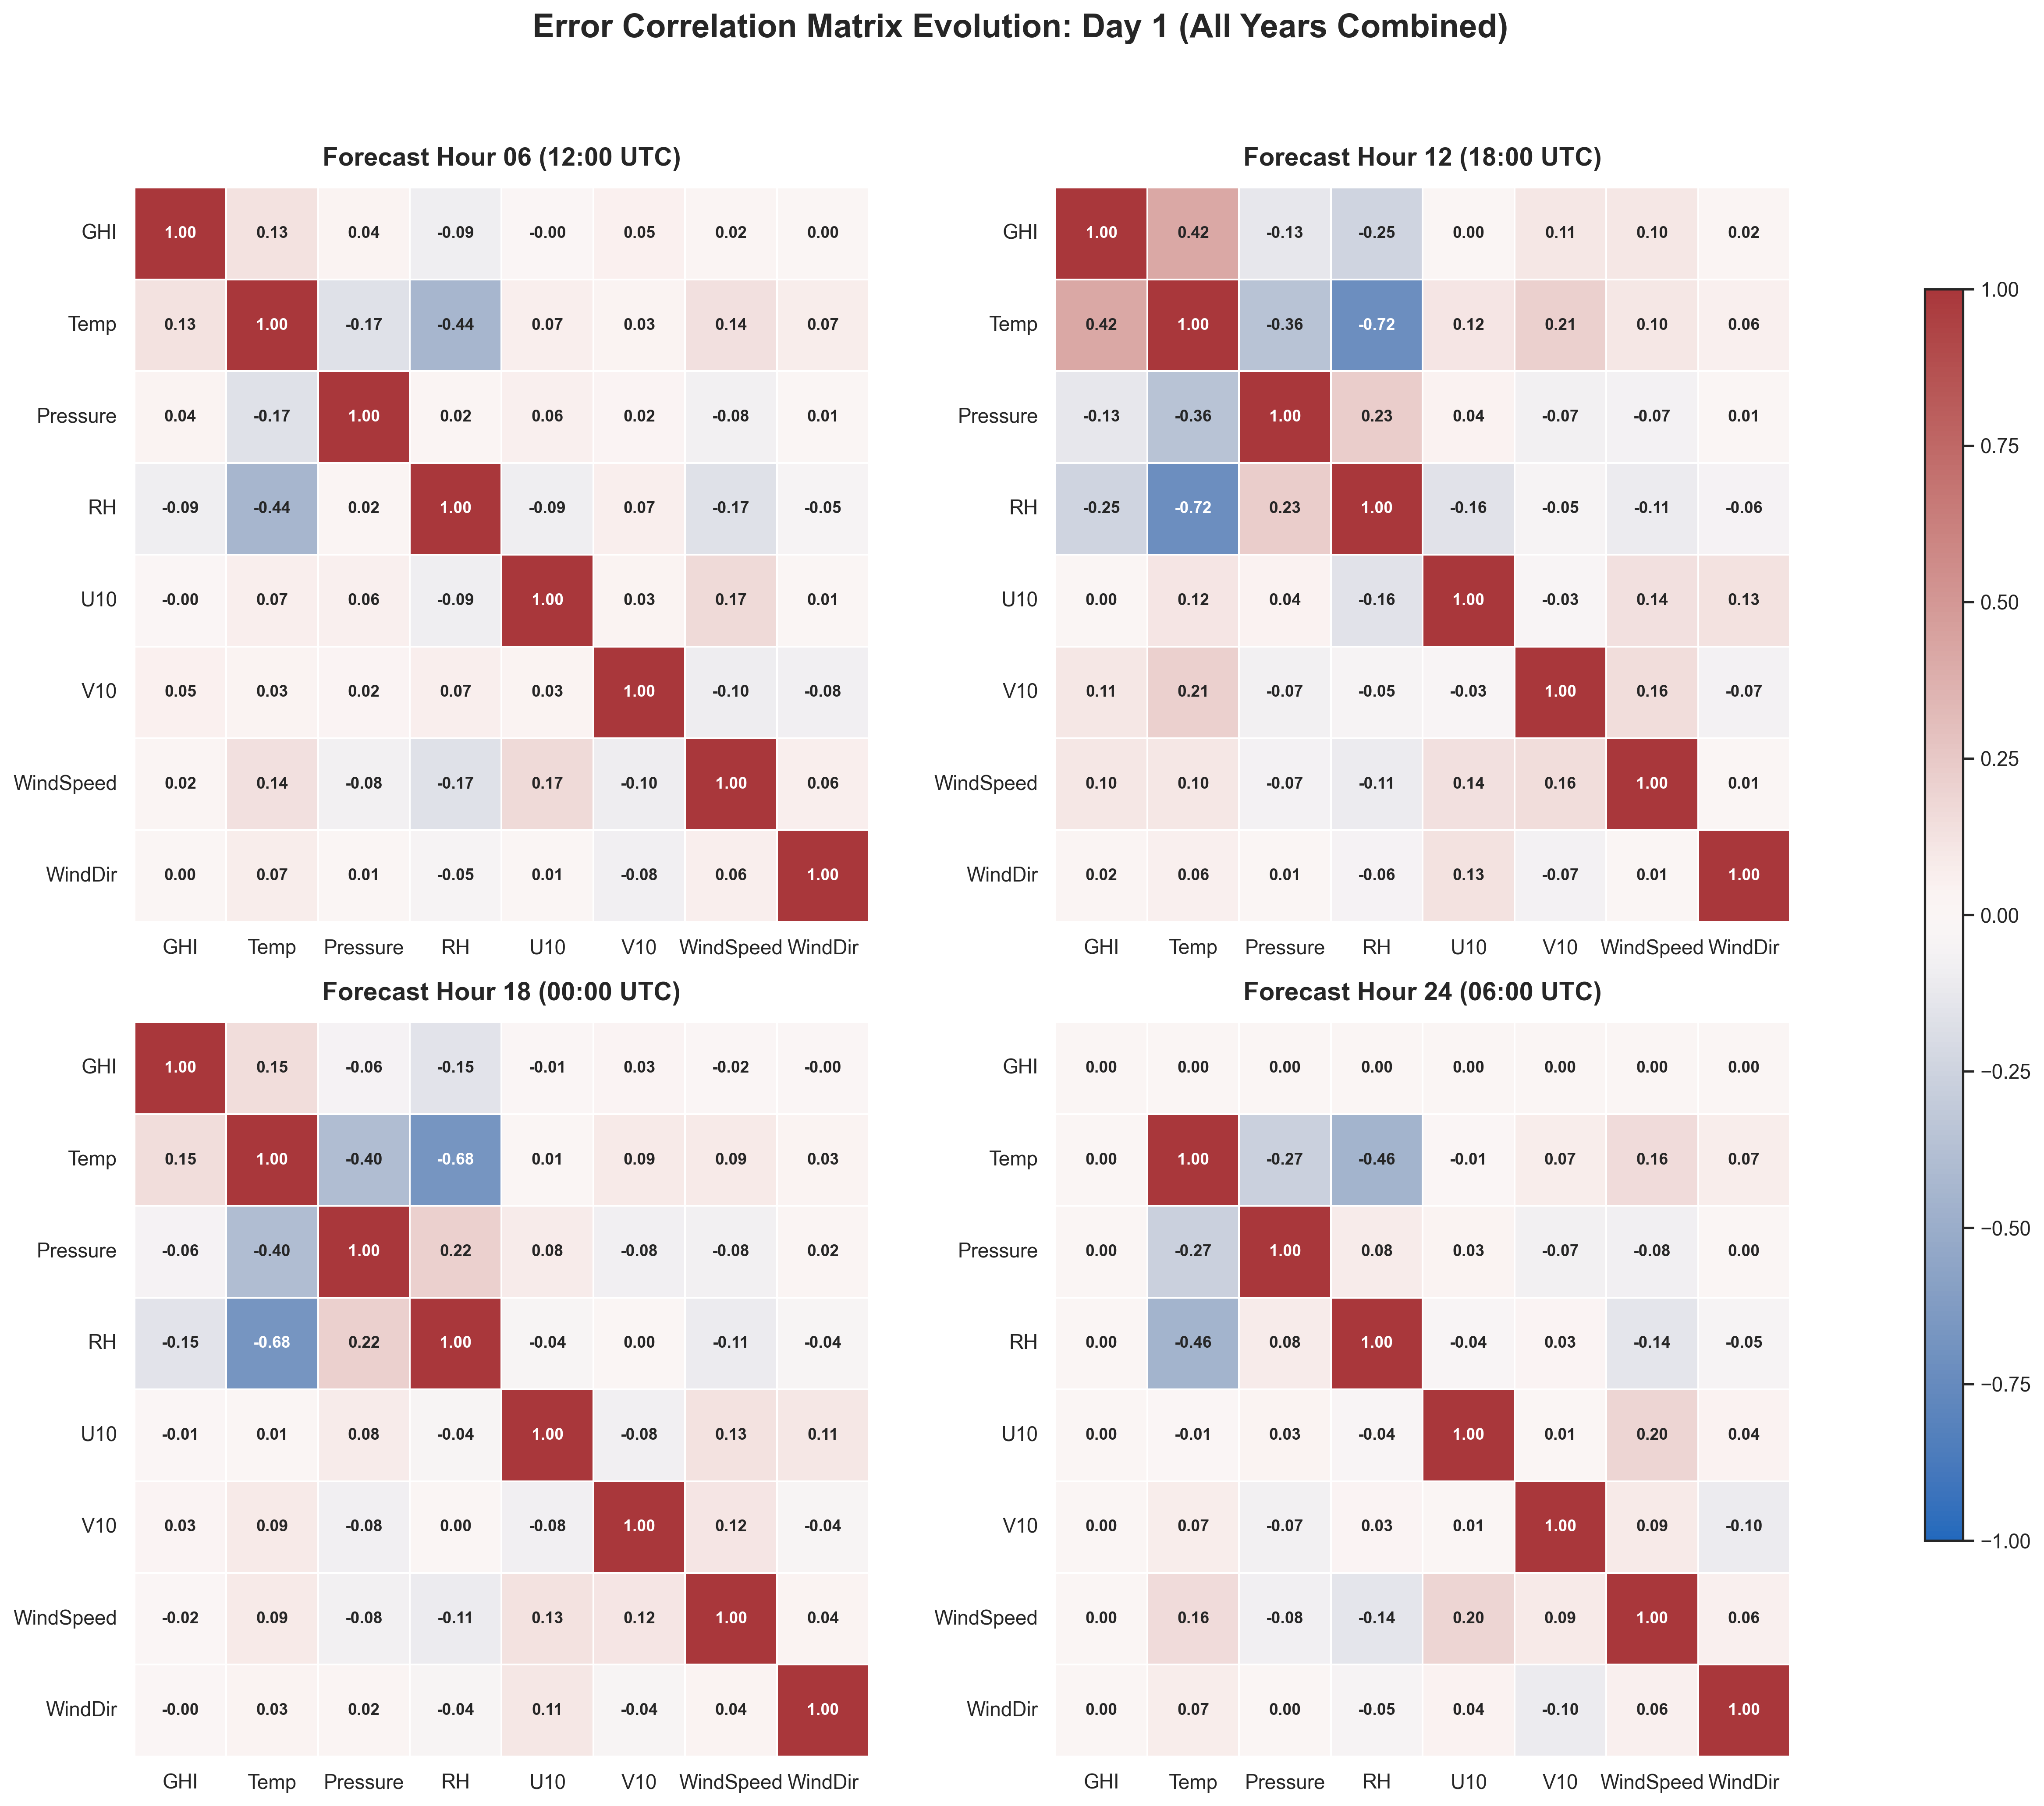
\includegraphics[width=\textwidth]{figures/Q7/TIMEOFDAY/all_variables_corr_day1_horizons.png}
  \caption{Faceted evolution of the cross-variable error Pearson correlation matrix at distinct forecast lead increments (Hours 06, 12, 18, and 24) across Forecast Day 1. The color bar indicates the Pearson $r$ value. The thermodynamic $T/\text{RH}$ coupling intensifies at solar noon (\texttt{18:00 UTC}), while daytime solar-noon GHI errors demonstrate strong phase-locked coupling with thermodynamic variables ($r_{\text{GHI}, T} = 0.42$, $r_{\text{GHI}, \text{RH}} = -0.25$) that completely evaporates at night.}
  \label{fig:cross_variable_diurnal_main}
\end{figure}

\subsection{Seasonal Variations}

In contrast to the rapid shifts observed within the diurnal cycle, the cross-variable error structures exhibit broad consistency across seasons, though specific thermodynamic couplings still experience notable variations. Seasonal matrices for Fall (Figure~\ref{fig:app_fall_day_night}), Spring (Figure~\ref{fig:app_spring_day_night}), Summer (Figure~\ref{fig:app_summer_day_night}), and Winter (Figure~\ref{fig:app_winter_day_night}) reveal that while the foundational structure of the errors remain similar, the intensity of these relationships changes with the seasonal solar and thermal cycle.

The most prominent seasonal difference occurs within the core thermodynamic temperature and relative humidity coupling. This inverse linear relationship is highly sensitive to seasonal characteristics:
\begin{itemize}
    \item \textbf{Summer (Figure~\ref{fig:app_summer_day_night}):} Features the most intense coupling, with daylight $T/\text{RH}$ error correlations reaching $r = -0.80$ and nighttime values at $r = -0.63$, potentially driven by high moisture and hotter surface heating.
    \item \textbf{Spring and Fall (Figure~\ref{fig:app_spring_day_night}, Figure~\ref{fig:app_fall_day_night}):} Display intermediate, nearly identical structural baselines, with Temperature / Relative Humidity (T/RH) couplings holding steady at $r = -0.69$ and $r = -0.68$, respectively. Night hours similarly do not drastically differ between Spring and Fall, with (T/RH) at $r = -0.54$ and $r = -0.52$, respectively. 
    \item \textbf{Winter (Figure~\ref{fig:app_winter_day_night}):} Experiences a significant loss in intensity of this coupling, dropping to a daylight low of $r = -0.51$ and a nighttime low of $r = -0.33$. This suppression points to the diminished role of temperature-driven moisture variations during cold, low humidity winter regimes.
\end{itemize}

Secondary variations emerge within the pressure-thermodynamic vectors. In the Summer matrix (Figure~\ref{fig:app_summer_day_night}), temperature and surface pressure errors are moderately coupled during the day ($r = -0.44$), matching a corresponding positive pressure-to-RH error link ($r = 0.32$). In the Winter matrix (Figure~\ref{fig:app_winter_day_night}), however, this pressure-temperature vector weakens to $r = -0.33$, while the pressure-to-RH error link collapses entirely to $r = 0.09$ across both diurnal phases. 

Conversely, daylight GHI-to-temperature error links remain remarkably stable across all matrices, fluctuating narrowly between a winter low of $r = 0.29$ (Figure~\ref{fig:app_winter_day_night}) and a spring high of $r = 0.38$ (Figure~\ref{fig:app_spring_day_night}). Wind variables (U10, V10, and Wind Speed) similarly preserve low, decoupled baseline correlations with thermodynamic vectors regardless of the season, indicating that the core spatial wind-prediction error structures remain disconnected from seasonal differences.

\subsection{Interannual Stability}

Year-to-year evaluations across 2022 (Figure~\ref{fig:app_corr_2022}), 2023 (Figure~\ref{fig:app_corr_2023}), and 2024 (Figure~\ref{fig:app_corr_2024}) reveal near-absolute statistical invariance in the cross-variable error structures. Core driving vectors exhibit virtually no annual fluctuations; for instance, the dominant daytime temperature and relative humidity ($T/\text{RH}$) error correlation remains locked between $r = -0.69$ and $r = -0.71$, while the nighttime tracking stays bound tightly between $r = -0.49$ and $r = -0.51$ across all three years. Similarly, secondary daylight links—such as the GHI-to-temperature coupling ($r \approx 0.31$ to $0.35$) and the inverse pressure-to-temperature coupling ($r \approx -0.28$ to $-0.33$)—remain structurally constant. This long-term stability demonstrates that multi-variable error distributions are insulated from yearly model drift.


\subsection{Regional and Zonal Variations}

When evaluated across the individual PJM geographic transmission zones—APS (Figure~\ref{fig:app_zone_aps}), ATSI (Figure~\ref{fig:app_zone_atsi}), COMD (Figure~\ref{fig:app_zone_comd}), DOM (Figure~\ref{fig:app_zone_dom}), EMAC (Figure~\ref{fig:app_zone_emac}), PENE (Figure~\ref{fig:app_zone_pene}), SMAC (Figure~\ref{fig:app_zone_smac}), West (Figure~\ref{fig:app_zone_west}), and WMAC (Figure~\ref{fig:app_zone_wmac})—the cross-variable error matrices exhibit notable spatial uniformity across the core Eastern Interconnection clusters, with a single distinct exception. 

For the eight geographically connected eastern and mid-Atlantic zones (spanning from Indianas border through Ohio, Pennsylvania, Maryland, and Virginia...), the baseline error couplings remain closely bounded. Across these eastern footprints, daylight $T/\text{RH}$ stays highly stable within a narrow range ($r \approx -0.69$ to $-0.74$), while daytime GHI to Temperature error links consistently hover between $r = 0.31$ and $r = 0.34$. 

The singular structural anomaly emerges within the Commonwealth Edison (COMD) zone matrix (Figure~\ref{fig:app_zone_comd}). Situated in northern Illinois, COMD sits at the far northwestern fringe of the PJM territory, geographically isolated from the dense eastern coastal cluster. In the COMD daylight matrix, the characteristic $T/\text{RH}$ inverse error correlation weakens significantly to $r = -0.64$, while the daytime pressure-to-temperature coupling attenuates to $r = -0.29$ compared to the fleet baseline (such as $r = -0.38$ in DOM). 

This localized divergence points towards a climate transition: while the eastern assets are bound to uniform, ocean-influenced or rolling Appalachian air masses, COMD’s boundary-layer errors are governed by the drier, more volatile continental climates of the upper Midwest. This localized shift suggests that while regional error profiles are largely static across the eastern footprint, far-western grid expansions introduce microclimate boundary conditions that require highly-localized joint error calibration.



\subsection{Findings and Implications}

The evaluation of the HRRR cross-variable error matrices reveals clear boundaries between highly dynamic weather factors and static, predictable baselines. These insights outline when and where joint error modeling matters most.

\begin{itemize}
    \item \textbf{Dominant Diurnal and Regional Drivers:} The most severe structural changes occur across the day/night cycle and at extreme geographic boundaries. Diurnal shifts alter the entire thermodynamic framework, creating complex error couplings (such as daytime GHI/T $r= 0.42$) that completely uncouple at night. Regionally, while error profiles are stable across the contiguous eastern PJM footprint, far-western zones like COMD introduce distinct microclimatic shifts that require localized joint calibrations.
    \item \textbf{Moderate Seasonal Scaling:} Seasonal transitions act as a scaling factor rather than a structural change. The fundamental orientation of the matrices remains intact, but the intensity of core thermodynamic variables differs alongside seasonal  humidity, peaking in Summer (T/RH $r = -0.80$) and dropping in Winter ( T/RH $r = -0.51$).
    \item \textbf{Negligible Interannual Drift:} Year-to-year cross-variable error distributions across 2022, 2023, and 2024 exhibit nearly absolute statistical invariance. This stability suggests that joint distributions looking at multi-year historical datasets remain highly reliable for forward-looking scheduling.
\end{itemize}

A key operational limitation of this framework is its reliance on Pearson correlation, which exclusively captures linear associations. Complex, non-linear physical thresholds between error vectors—such as an error in one variable triggering an order-of-magnitude leap in another—remain unquantified by this metric. Future iterations of this risk-modeling framework could leverage non-linear regression techniques or copula-based joint distributions to more accurately map threshold-dependent error behavior under extreme grid scenarios.


% ======================================================================
\section{Q8 — Spatial Correlation Across PJM Zones}\label{sec:spatial}
% ======================================================================

A geographically distributed fleet only smooths forecast errors if they are spatially independent. To assess spatial independence, we measure the spatial coherence by computing (i) zone-to-zone correlation, and (ii) the distance over which site-to-site correlation decays.

\subsection{Zone-to-zone correlation}

We collapse the \num{896} sites into their nine PJM zones, form a zone-mean error series
per zone (all lead times pooled), and Pearson-correlate the nine series per variable
(Figure~\ref{fig:zonecorr}).

\begin{figure}[H]
  \centering
  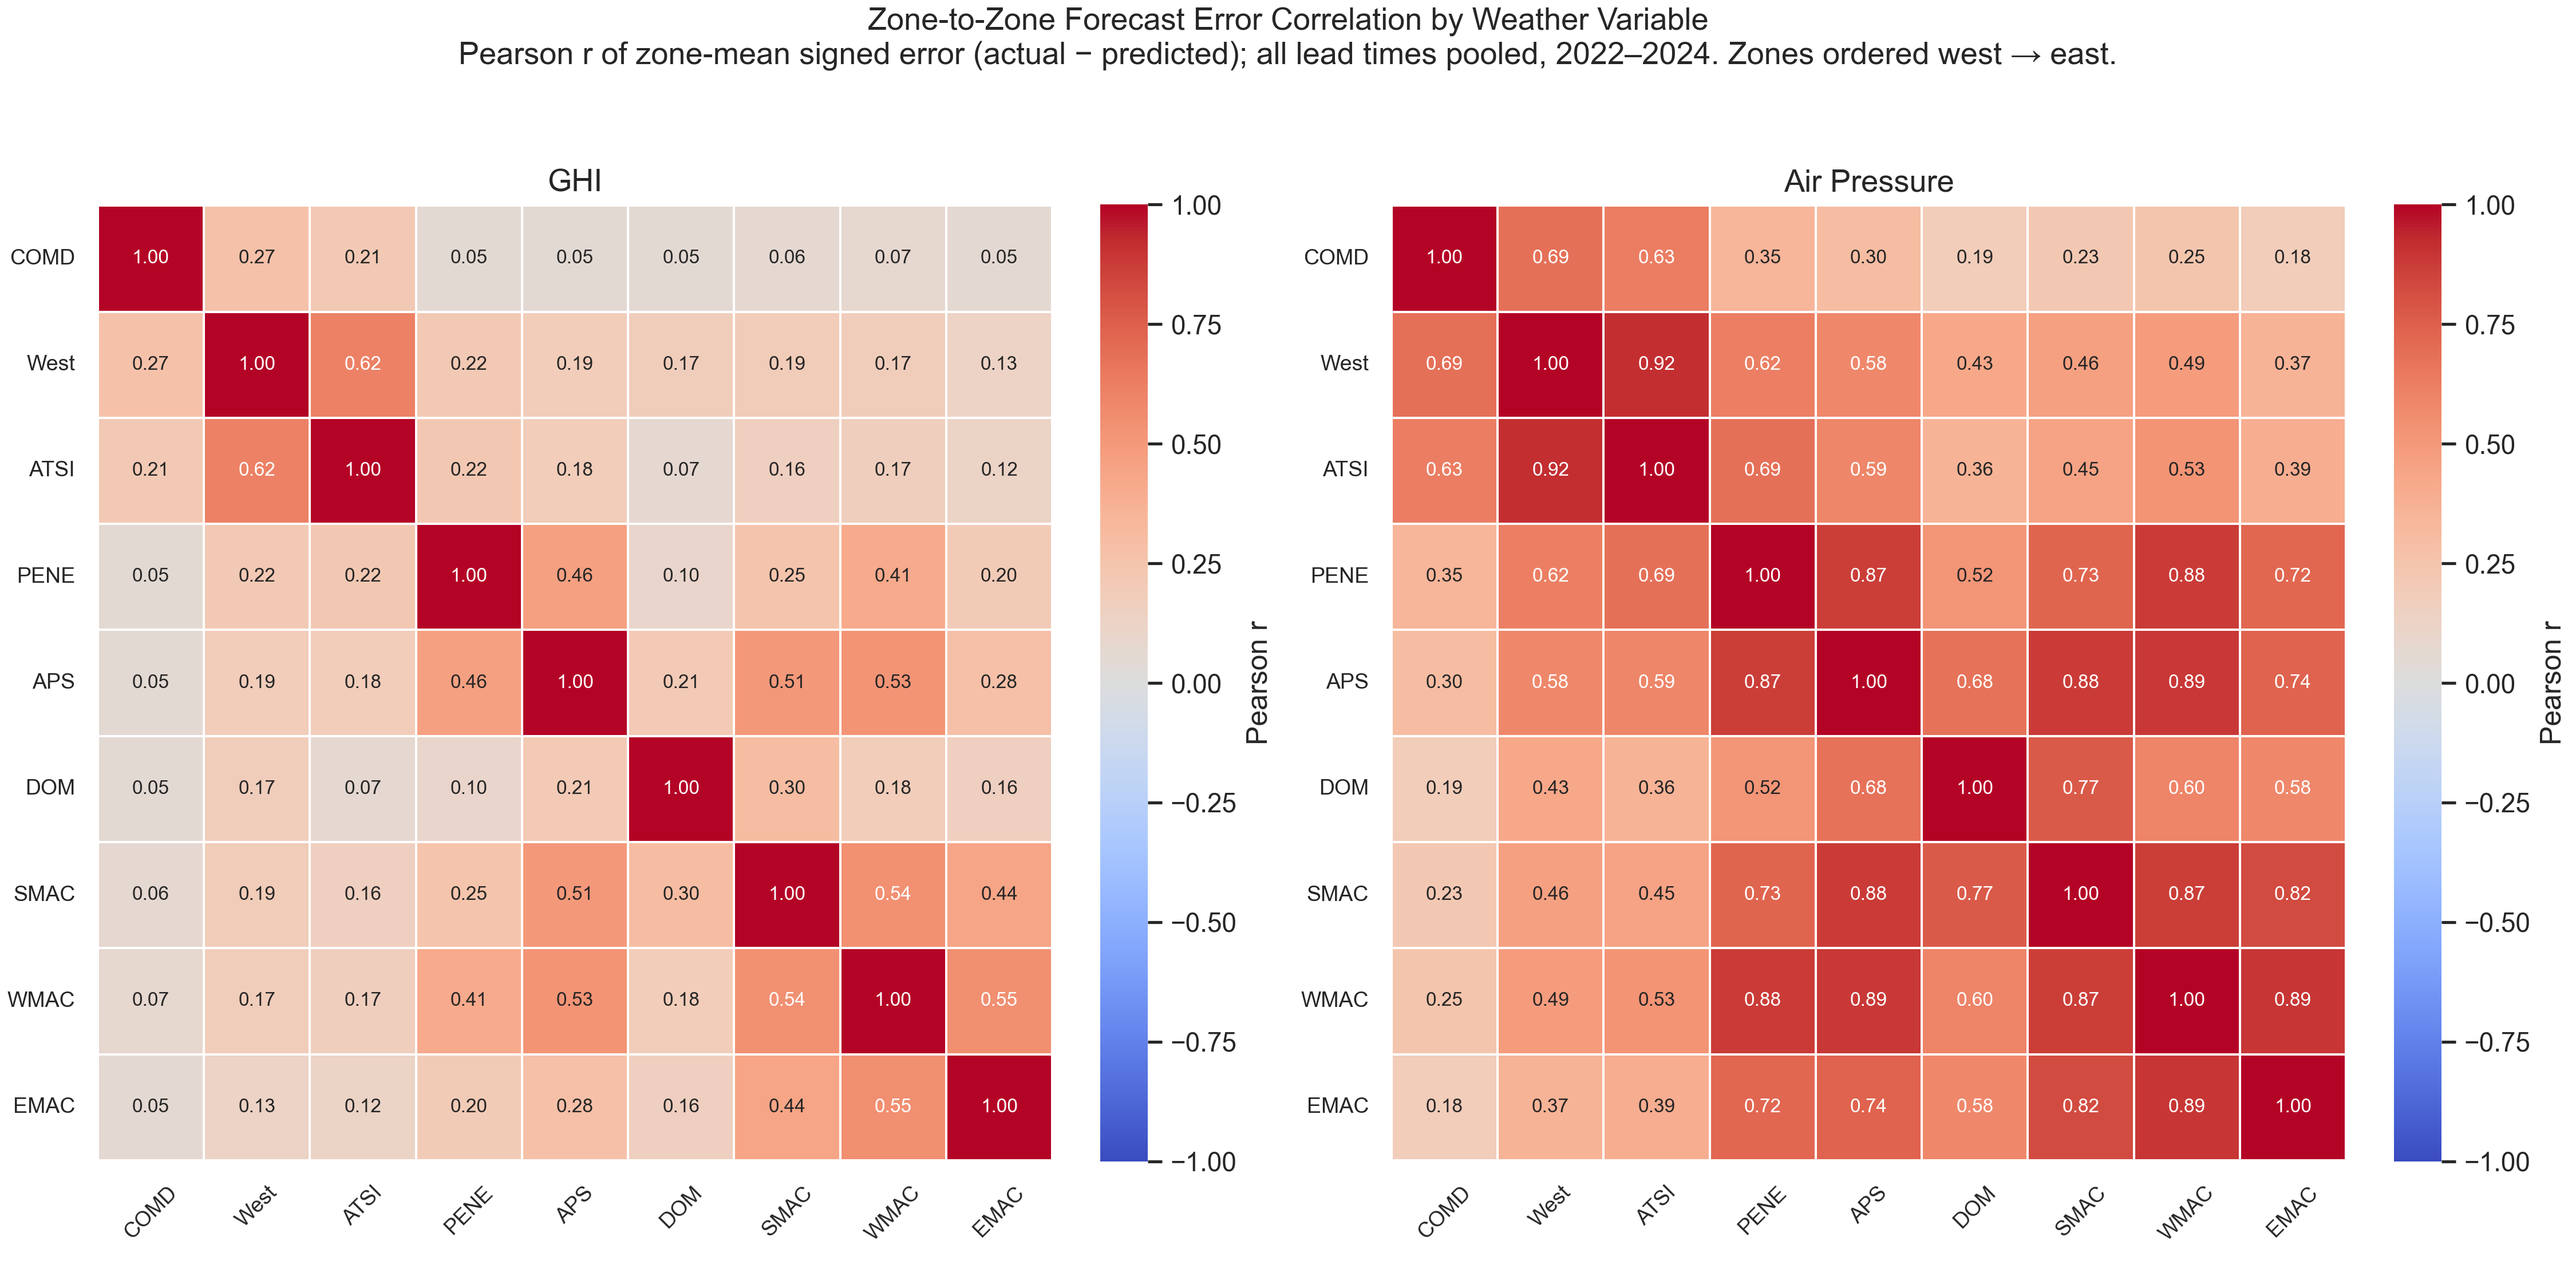
\includegraphics[width=\textwidth]{figures/Q8/embed/zone_error_correlation_ghi_pressure copy.png}
  \caption{Zone-to-zone forecast-error correlation, one $9\times 9$ matrix per variable, with
  zones ordered west~$\rightarrow$~east. Warmer off-diagonal cells indicate zones whose errors
  move together. Pressure is the warmest matrix (synoptic, regionally coherent); wind direction
  is the coolest (near-zero everywhere); GHI is also cool (local, cloud-driven). Within every
  variable the strongest correlations cluster near the diagonal, reflecting geographic adjacency.}
  \label{fig:zonecorr}
\end{figure}

Ranking variables by mean off-diagonal correlation gives, from most to least coherent:
air pressure (0.59) $>$ RH (0.56) $>$ temperature (0.41) $>$ U10 (0.27) $>$ GHI (0.24) $>$
V10 (0.22) $>$ wind speed (0.19) $>$ wind direction (0.08). Air pressure is the most spatially
coherent---neighboring zones correlate at 0.6--0.9---because pressure errors are at a synoptic scale.
GHI and wind direction are the most independent across zones.

\subsection{Spatial decay and the decorrelation length}

For a fixed lead time we compute, for every one of the $\approx \num{400000}$ site pairs, the
great-circle distance and the Pearson correlation of their signed-error series. Binning the pairs
into \SI{25}{km} distance bins and fitting an exponential
$\rho(d) = a\,e^{-d/L} + c$ yields the \emph{decorrelation length} $L$ (the e-folding distance at
which the decaying part falls to $1/e \approx 37\%$). Figure~\ref{fig:decay12} shows the headline
fit at lead~12 (solar noon).

\begin{figure}[H]
  \centering
  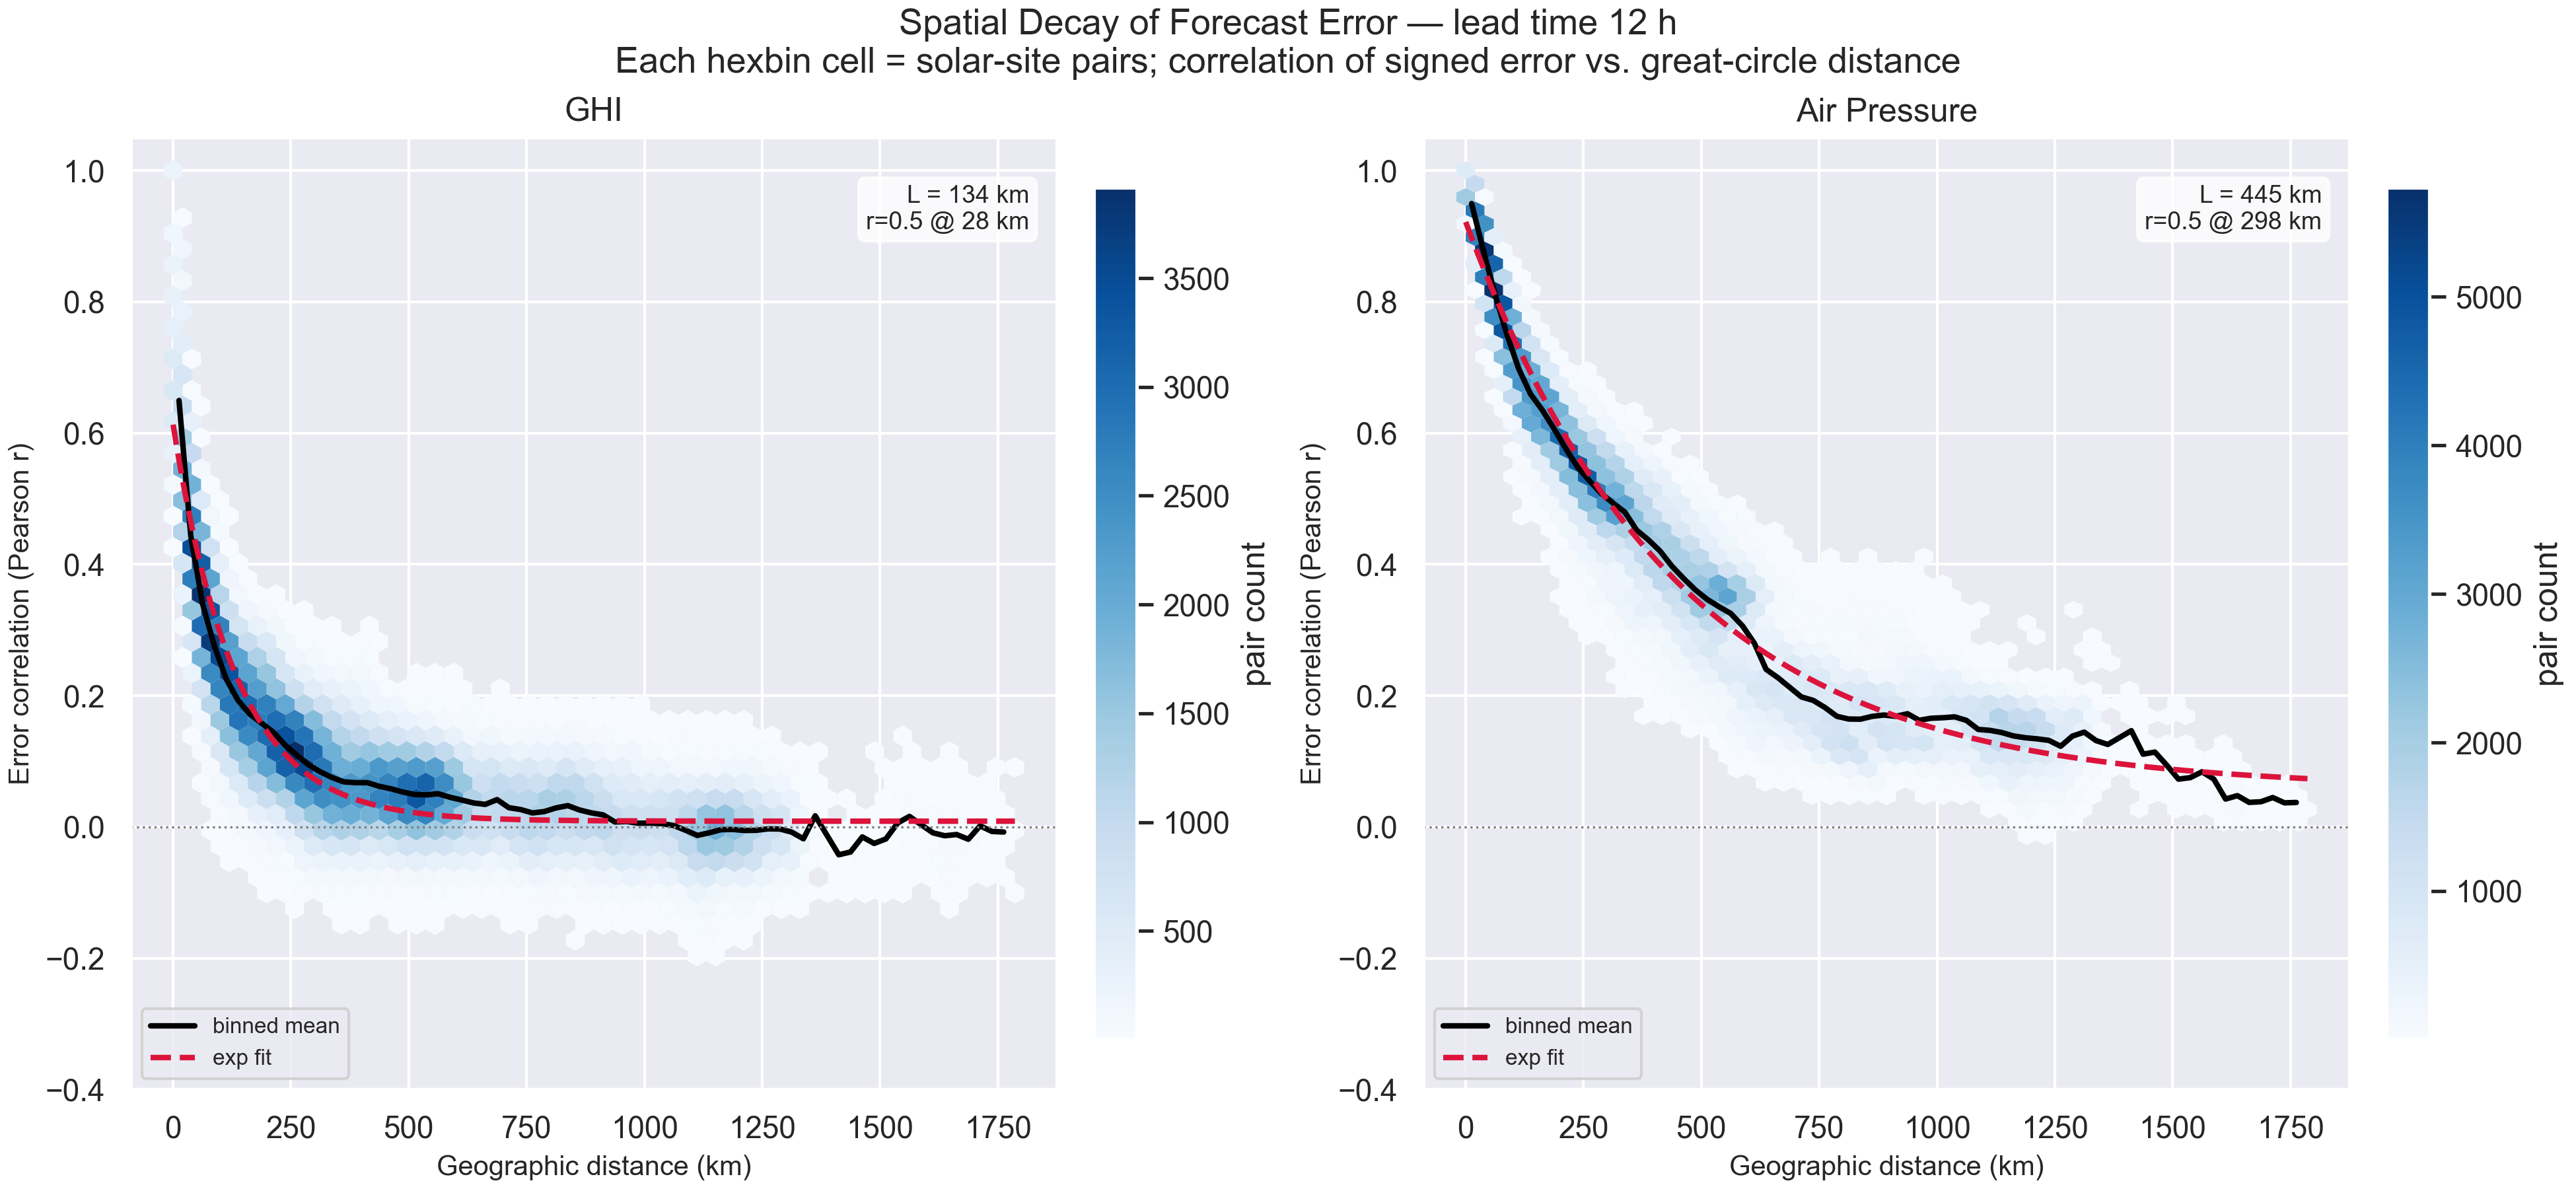
\includegraphics[width=\textwidth]{figures/Q8/embed/spatial_decay_lead12_ghi_pressure.png}
  \caption{Spatial decay of forecast error at lead~12~h (= \texttt{18z}, solar noon). Each panel
  plots error correlation versus great-circle distance for all $\approx\num{400000}$ site pairs
  (hexbin density), with the distance-binned mean (black) and fitted exponential
  $\rho(d)=a\,e^{-d/L}+c$ (crimson). Pressure is the most spatially coherent
  ($L \approx \SI{445}{km}$); temperature ($L \approx \SI{233}{km}$) and RH
  ($L \approx \SI{277}{km}$) are intermediate; GHI decorrelates fastest
  ($L \approx \SI{134}{km}$, $r=0.5$ by $\sim\SI{28}{km}$); wind direction is so noisy its fit
  never reaches $r=0.5$.}
  \label{fig:decay12}
\end{figure}

\subsection{Implications}

Forecast errors only diversify across a portfolio when sites are spaced \emph{farther apart than
$L$}. Because $L$ is shortest for GHI and wind direction, a geographically spread fleet smooths
those errors well, and that is favorable since GHI drives solar output. Pressure and
temperature errors, by contrast, stay correlated across hundreds of kilometres and barely
diversify even fleet-wide.

As lead time increases, forecast errors for most variables become spatially correlated over longer distances, so aggregating sites levels out the total error less. Thus, the portfolio gets a smaller diversification benefit because more of the fleet is wrong in the same direction at the same time. However, forecasts errors for U10 and V10 trend downward, so the errors for longer lead times are more spatially independent.

The diurnal pattern observed in U10, GHI, and wind direction indicate that time of day is a confounding variable. Data for forecasts at different initialized times is necessary to investigate this further. Regardless, this finding indicates that errors are more spatially independent during the night.

% ======================================================================
\section{Q9 — Spatial Correlation Variation by Stratum}\label{sec:strata}
% ======================================================================

We repeated the spatial analyses but now \emph{within strata} (UTC hour of day, season,
and year) to test whether coherence is stable across them. The answer is \textbf{yes for season and time of
day, but no for year}.

\subsection{Season: the strongest effect}

Coherence and decorrelation length both collapse in summer and peak in the transition seasons and
autumn (Figure~\ref{fig:seasondecay}): temperature $L$ falls from $\sim\SI{348}{km}$ (Fall) to
$\sim\SI{119}{km}$ (Summer), RH from $\sim\SI{284}{km}$ to $\sim\SI{88}{km}$, and V10 from
$\sim\SI{602}{km}$ to $\sim\SI{114}{km}$. This indicates that summer errors are more local, so they
decorrelate over much shorter distances. Pressure is the exception, remaining synoptic
(\,$L \approx \SI{443}{km}$) all year.

\begin{figure}[H]
  \centering
  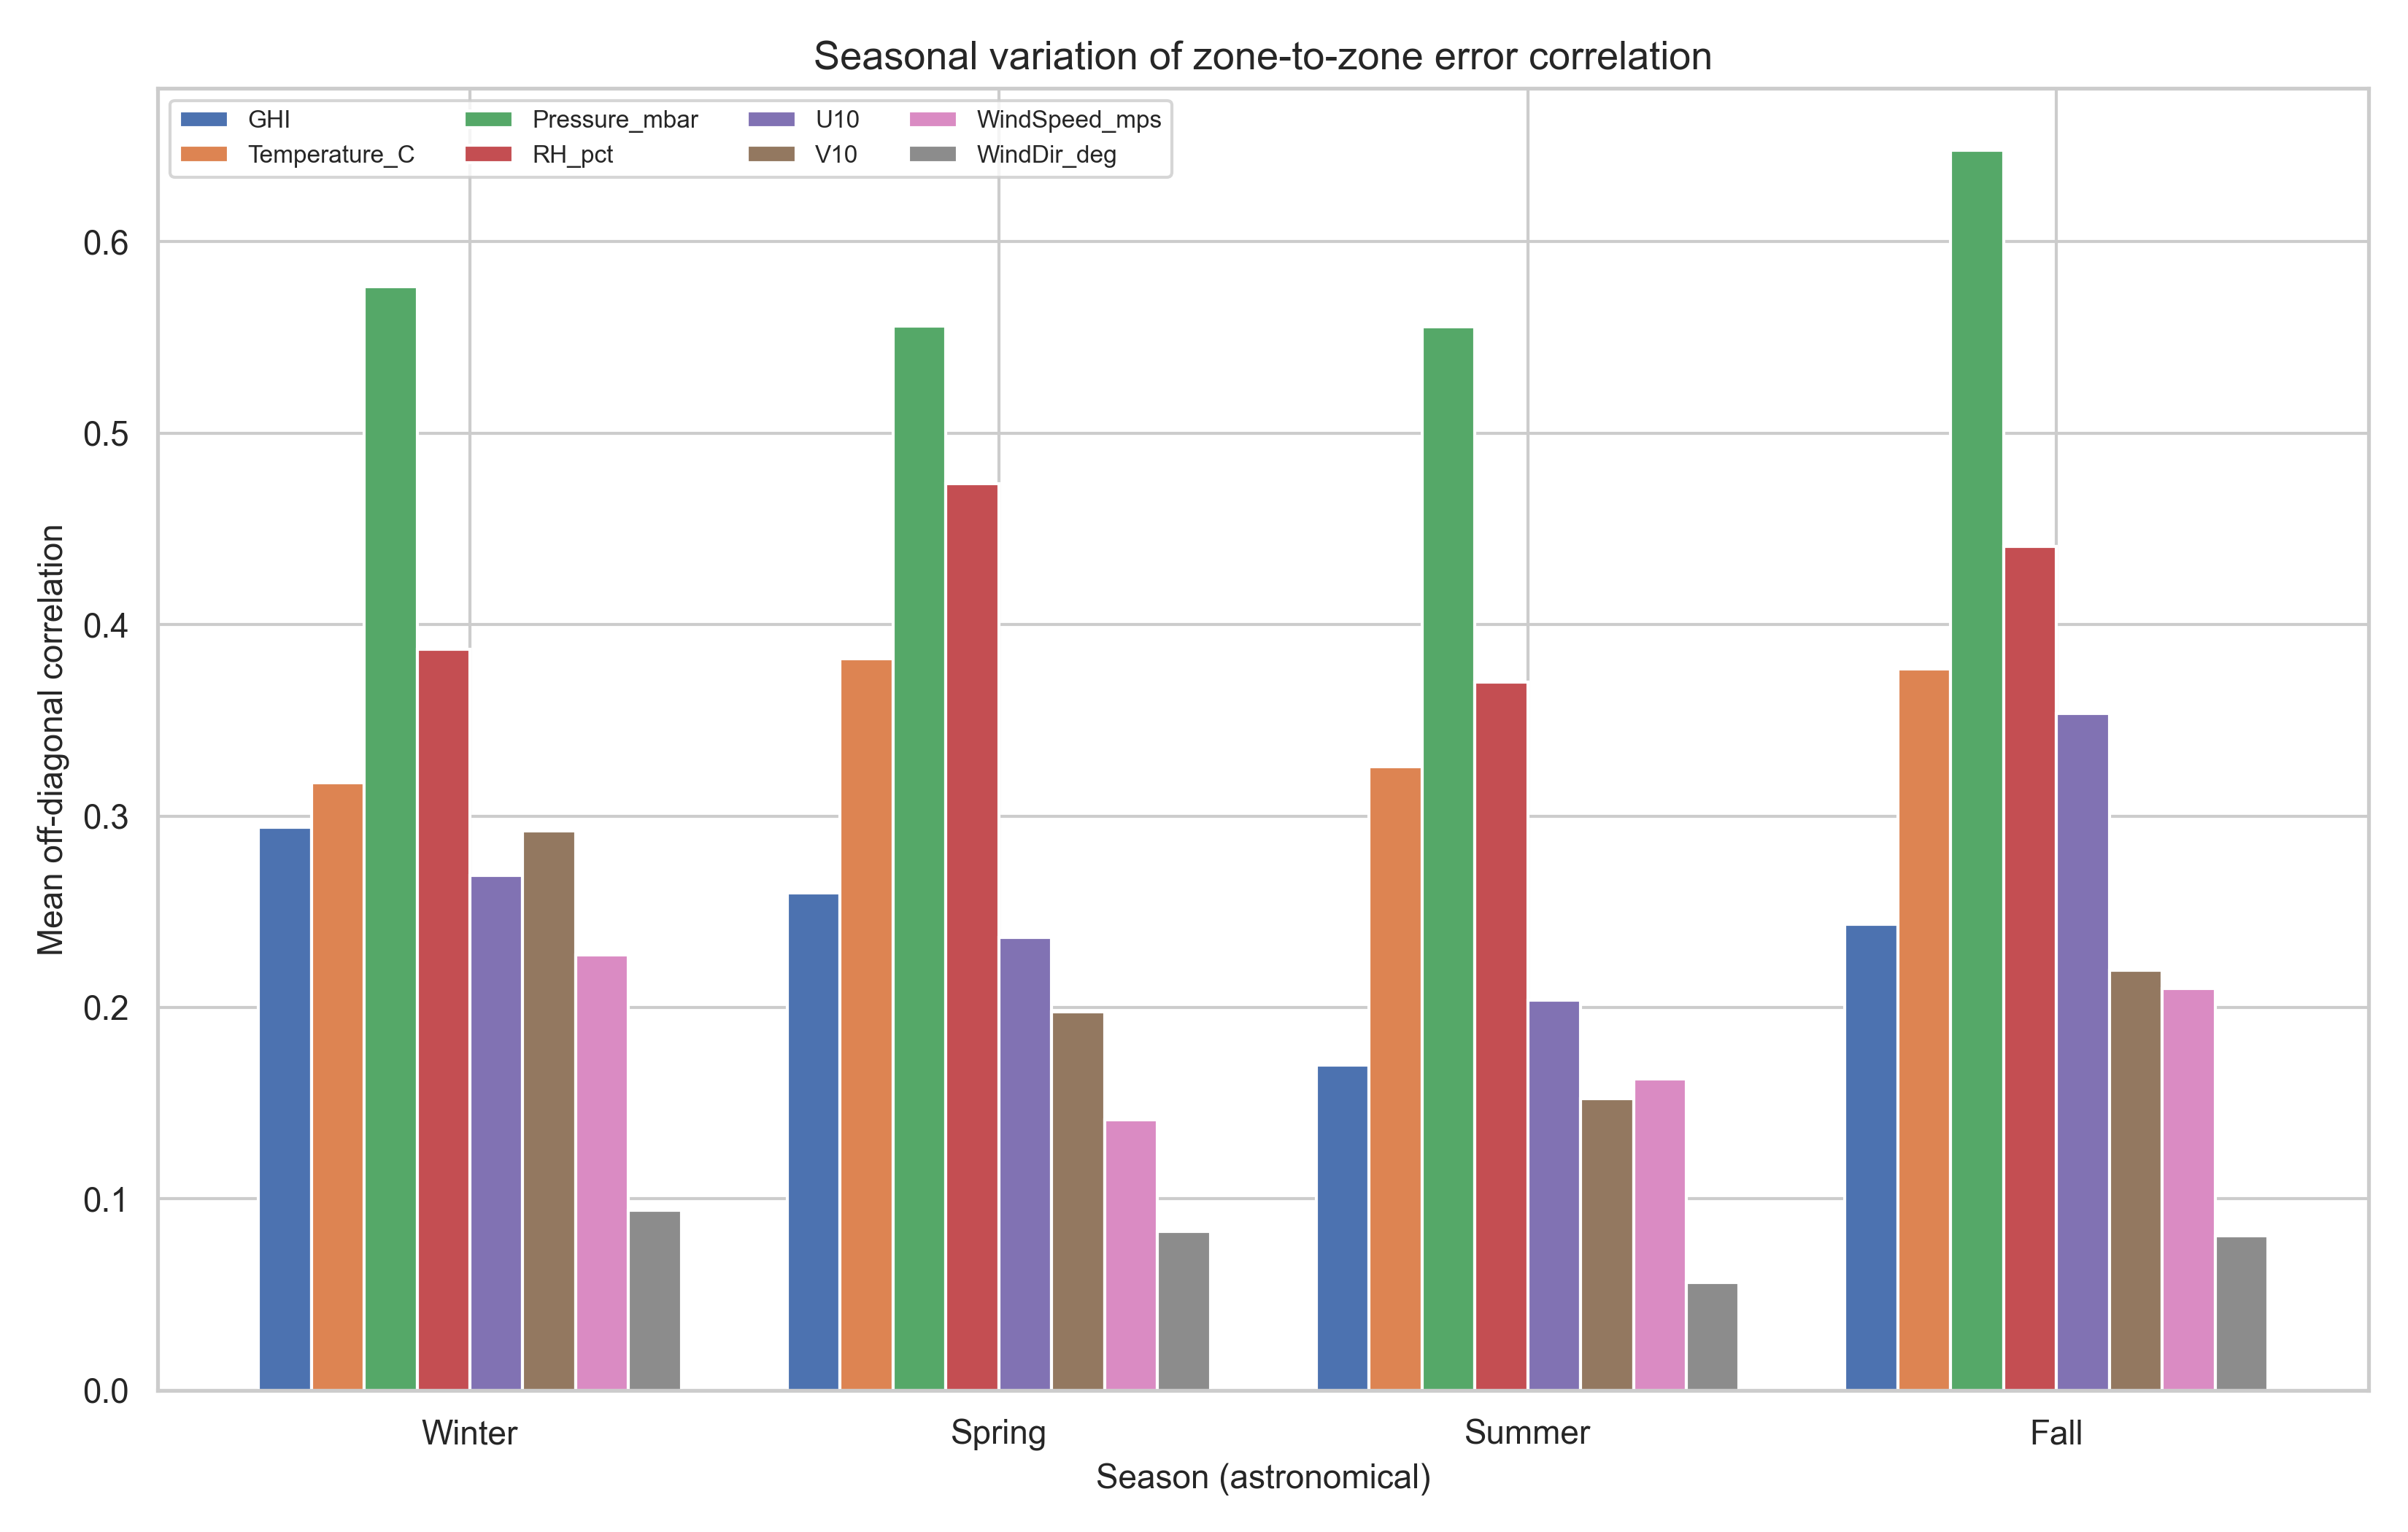
\includegraphics[width=\textwidth]{figures/Q9/seasonal_zone_correlation.png}
  \caption{Mean zone-to-zone correlation by season. Coherence is lowest in summer for every
  variable and highest in fall/winter; pressure and RH stay the most cross-zone coherent
  throughout. Summer is therefore the season in which neighbouring zones' errors are most
  independent.}
  \label{fig:seasoncorr}
\end{figure}

\begin{figure}[H]
  \centering
  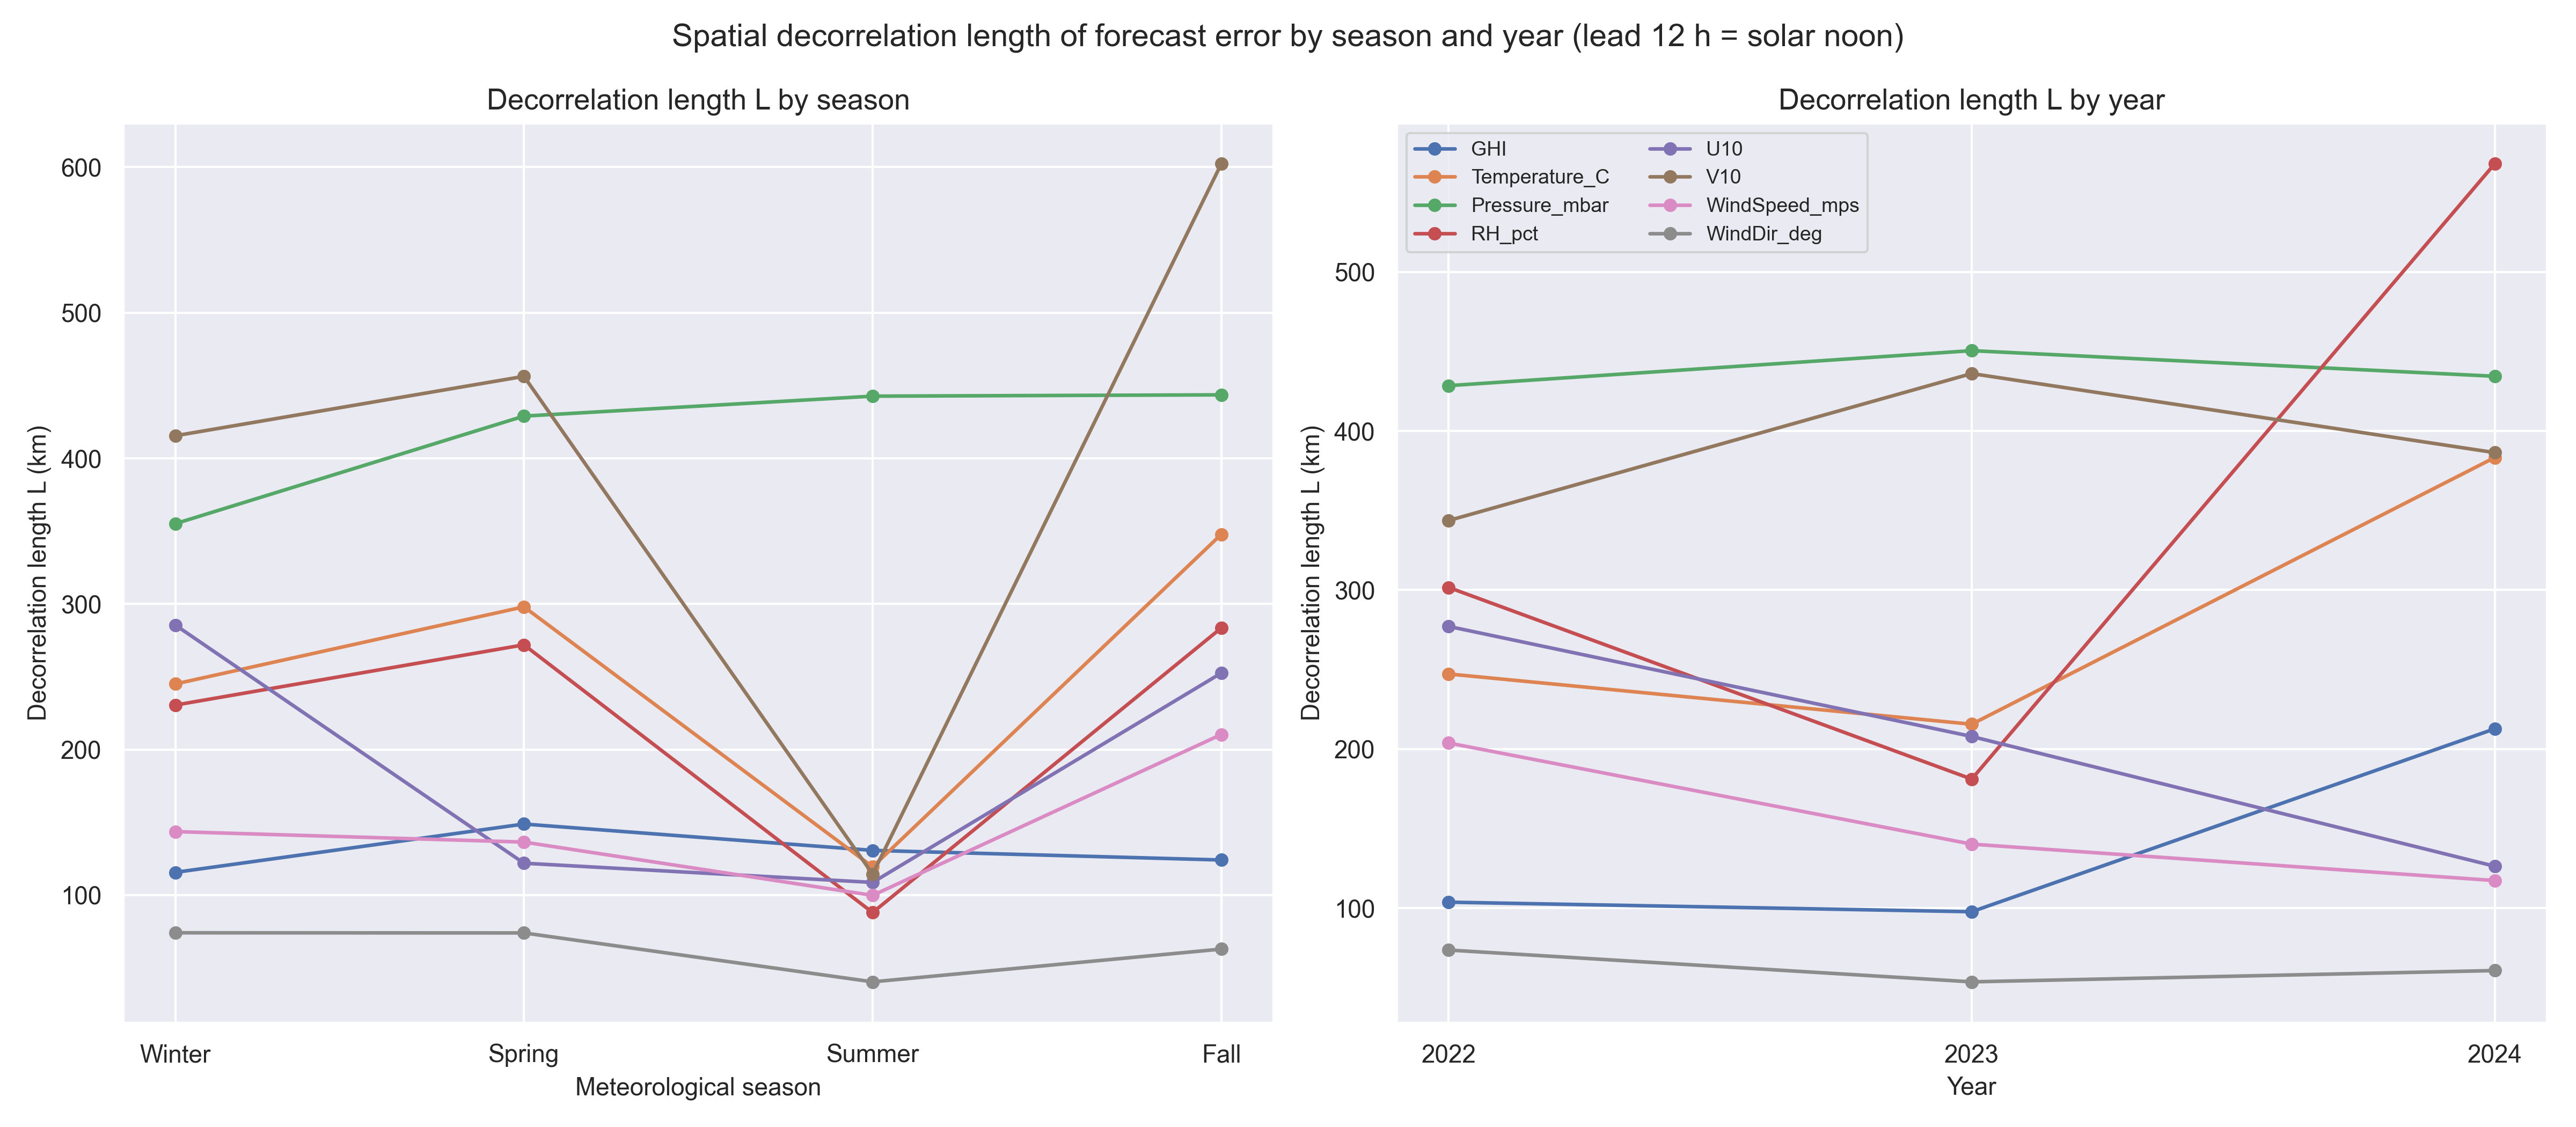
\includegraphics[width=\textwidth]{figures/Q9/decorrelation_length_by_season_year.png}
  \caption{Fitted decorrelation length $L$ by season (left) and year (right). $L$ collapses in
  summer as errors go local/convective, while pressure stays synoptic all year. The year panel is
  flat for pressure but swings 2--3$\times$ for RH/GHI/winds; a day-block bootstrap shows those
  year-to-year swings are within sampling uncertainty (see text).}
  \label{fig:seasondecay}
\end{figure}

\subsection{Time of day: a clear diurnal cycle}

Temperature and RH zone coherence dip in the mid-morning UTC hours
($\sim\!10\text{--}\SI{11}{}z$, the sunrise period) and rebound by late
afternoon ($\sim\!\SI{18}{}z$); pressure is flat across the day; GHI exists only in daytime UTC
hours and is modestly higher near solar noon; wind direction sits at a flat low floor
($\approx 0.08$). See Figure~\ref{fig:diurnal}.

\begin{figure}[H]
  \centering
  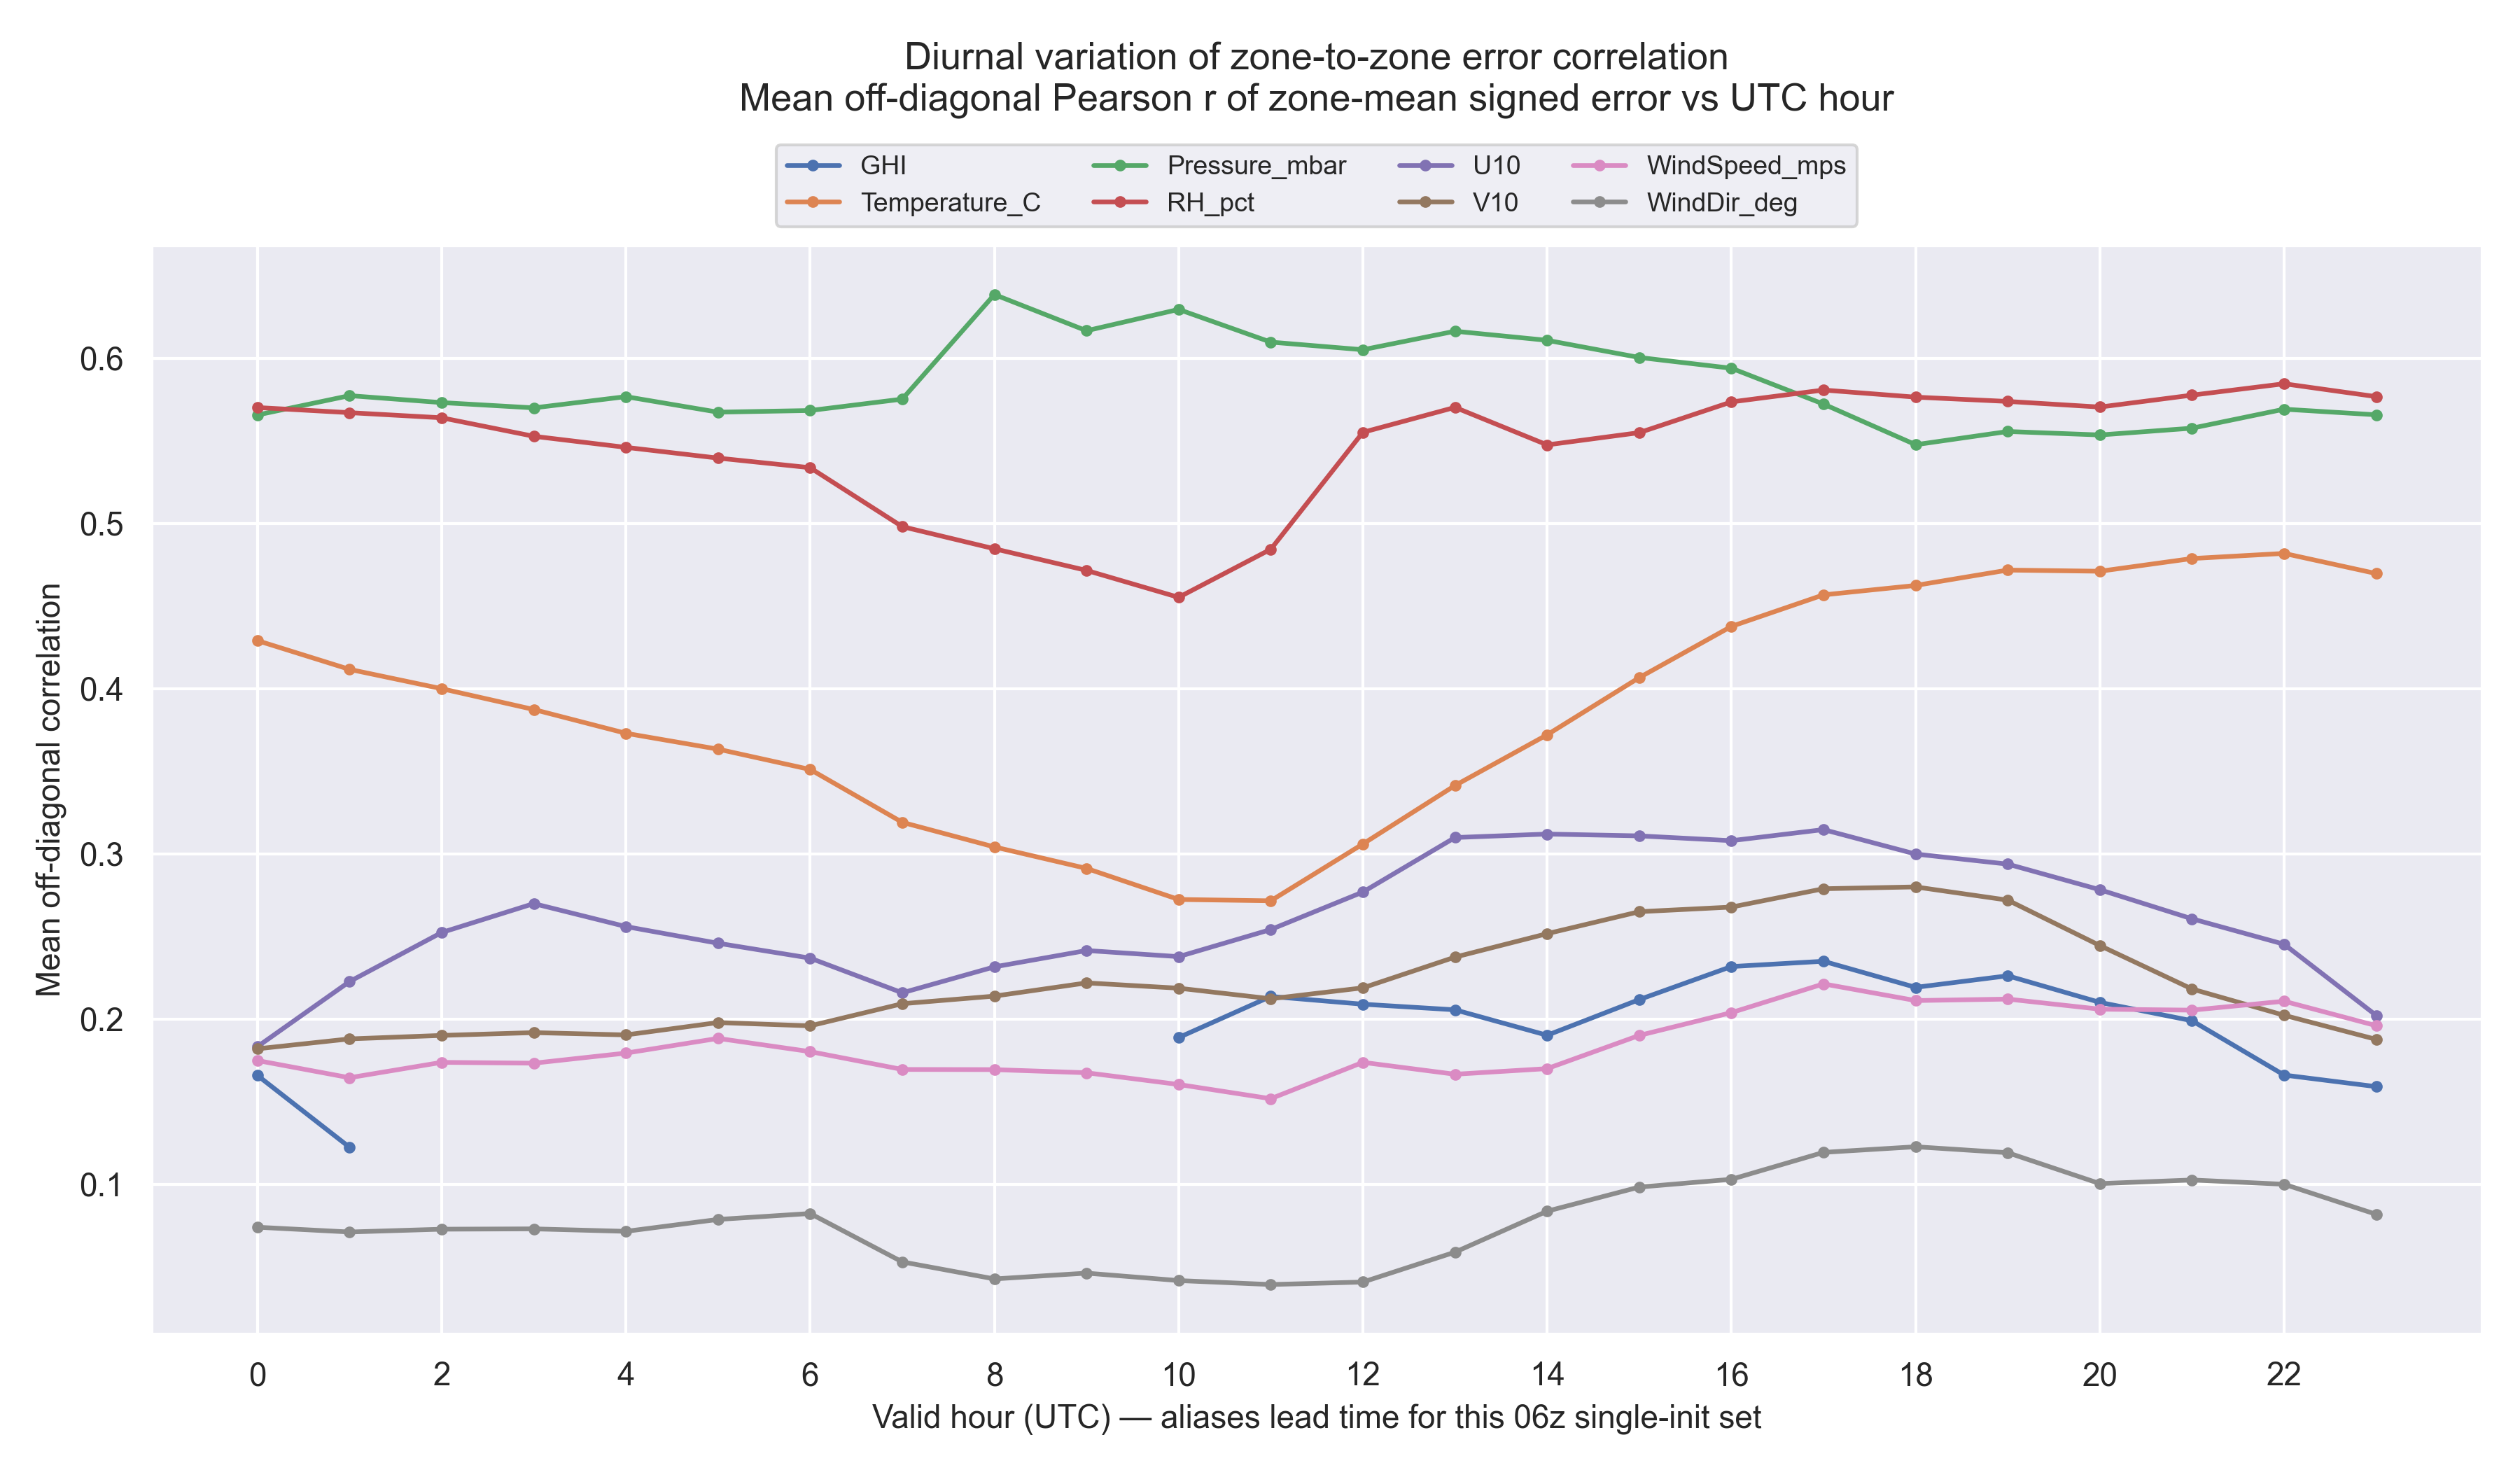
\includegraphics[width=\textwidth]{figures/Q9/diurnal_zone_correlation.png}
  \caption{Mean zone-to-zone correlation versus UTC hour. Temperature/RH coherence dips near
  sunrise (\,$\sim\!10\text{--}\SI{11}{}z$) and recovers by afternoon; pressure is flat; GHI is
  daytime-only and peaks near solar noon; wind direction is a flat low floor.}
  \label{fig:diurnal}
\end{figure}

\subsection{Year: stable, with a caveat on $L$}

The robust measures are flat across 2022--2024 (Figure~\ref{fig:yearcorr}): zone correlation moves only a few hundredths
(e.g.\ pressure $0.585 \to 0.571 \to 0.605$) and $d(r{=}0.5)$ is steady for clean-decay variables
, e.g. pressure $\sim\!294\text{--}\SI{304}{km}$. Although the \emph{fitted} $L$ swings 2--3$\times$ for the weakly-coherent variables (RH $302\to181\to\SI{568}{km}$; GHI $104\to98\to\SI{213}{km}$), a
day-block bootstrap shows the within-year sampling uncertainty is as large as those gaps. Hence, the
dramatic 2024 spikes across several variables sit only $\sim$1--1.6$\sigma$ above the other years and are not
significant. \textbf{Therefore, year-to-year changes in $L$ should not be read as real change between years}.

\begin{figure}[H]
  \centering
  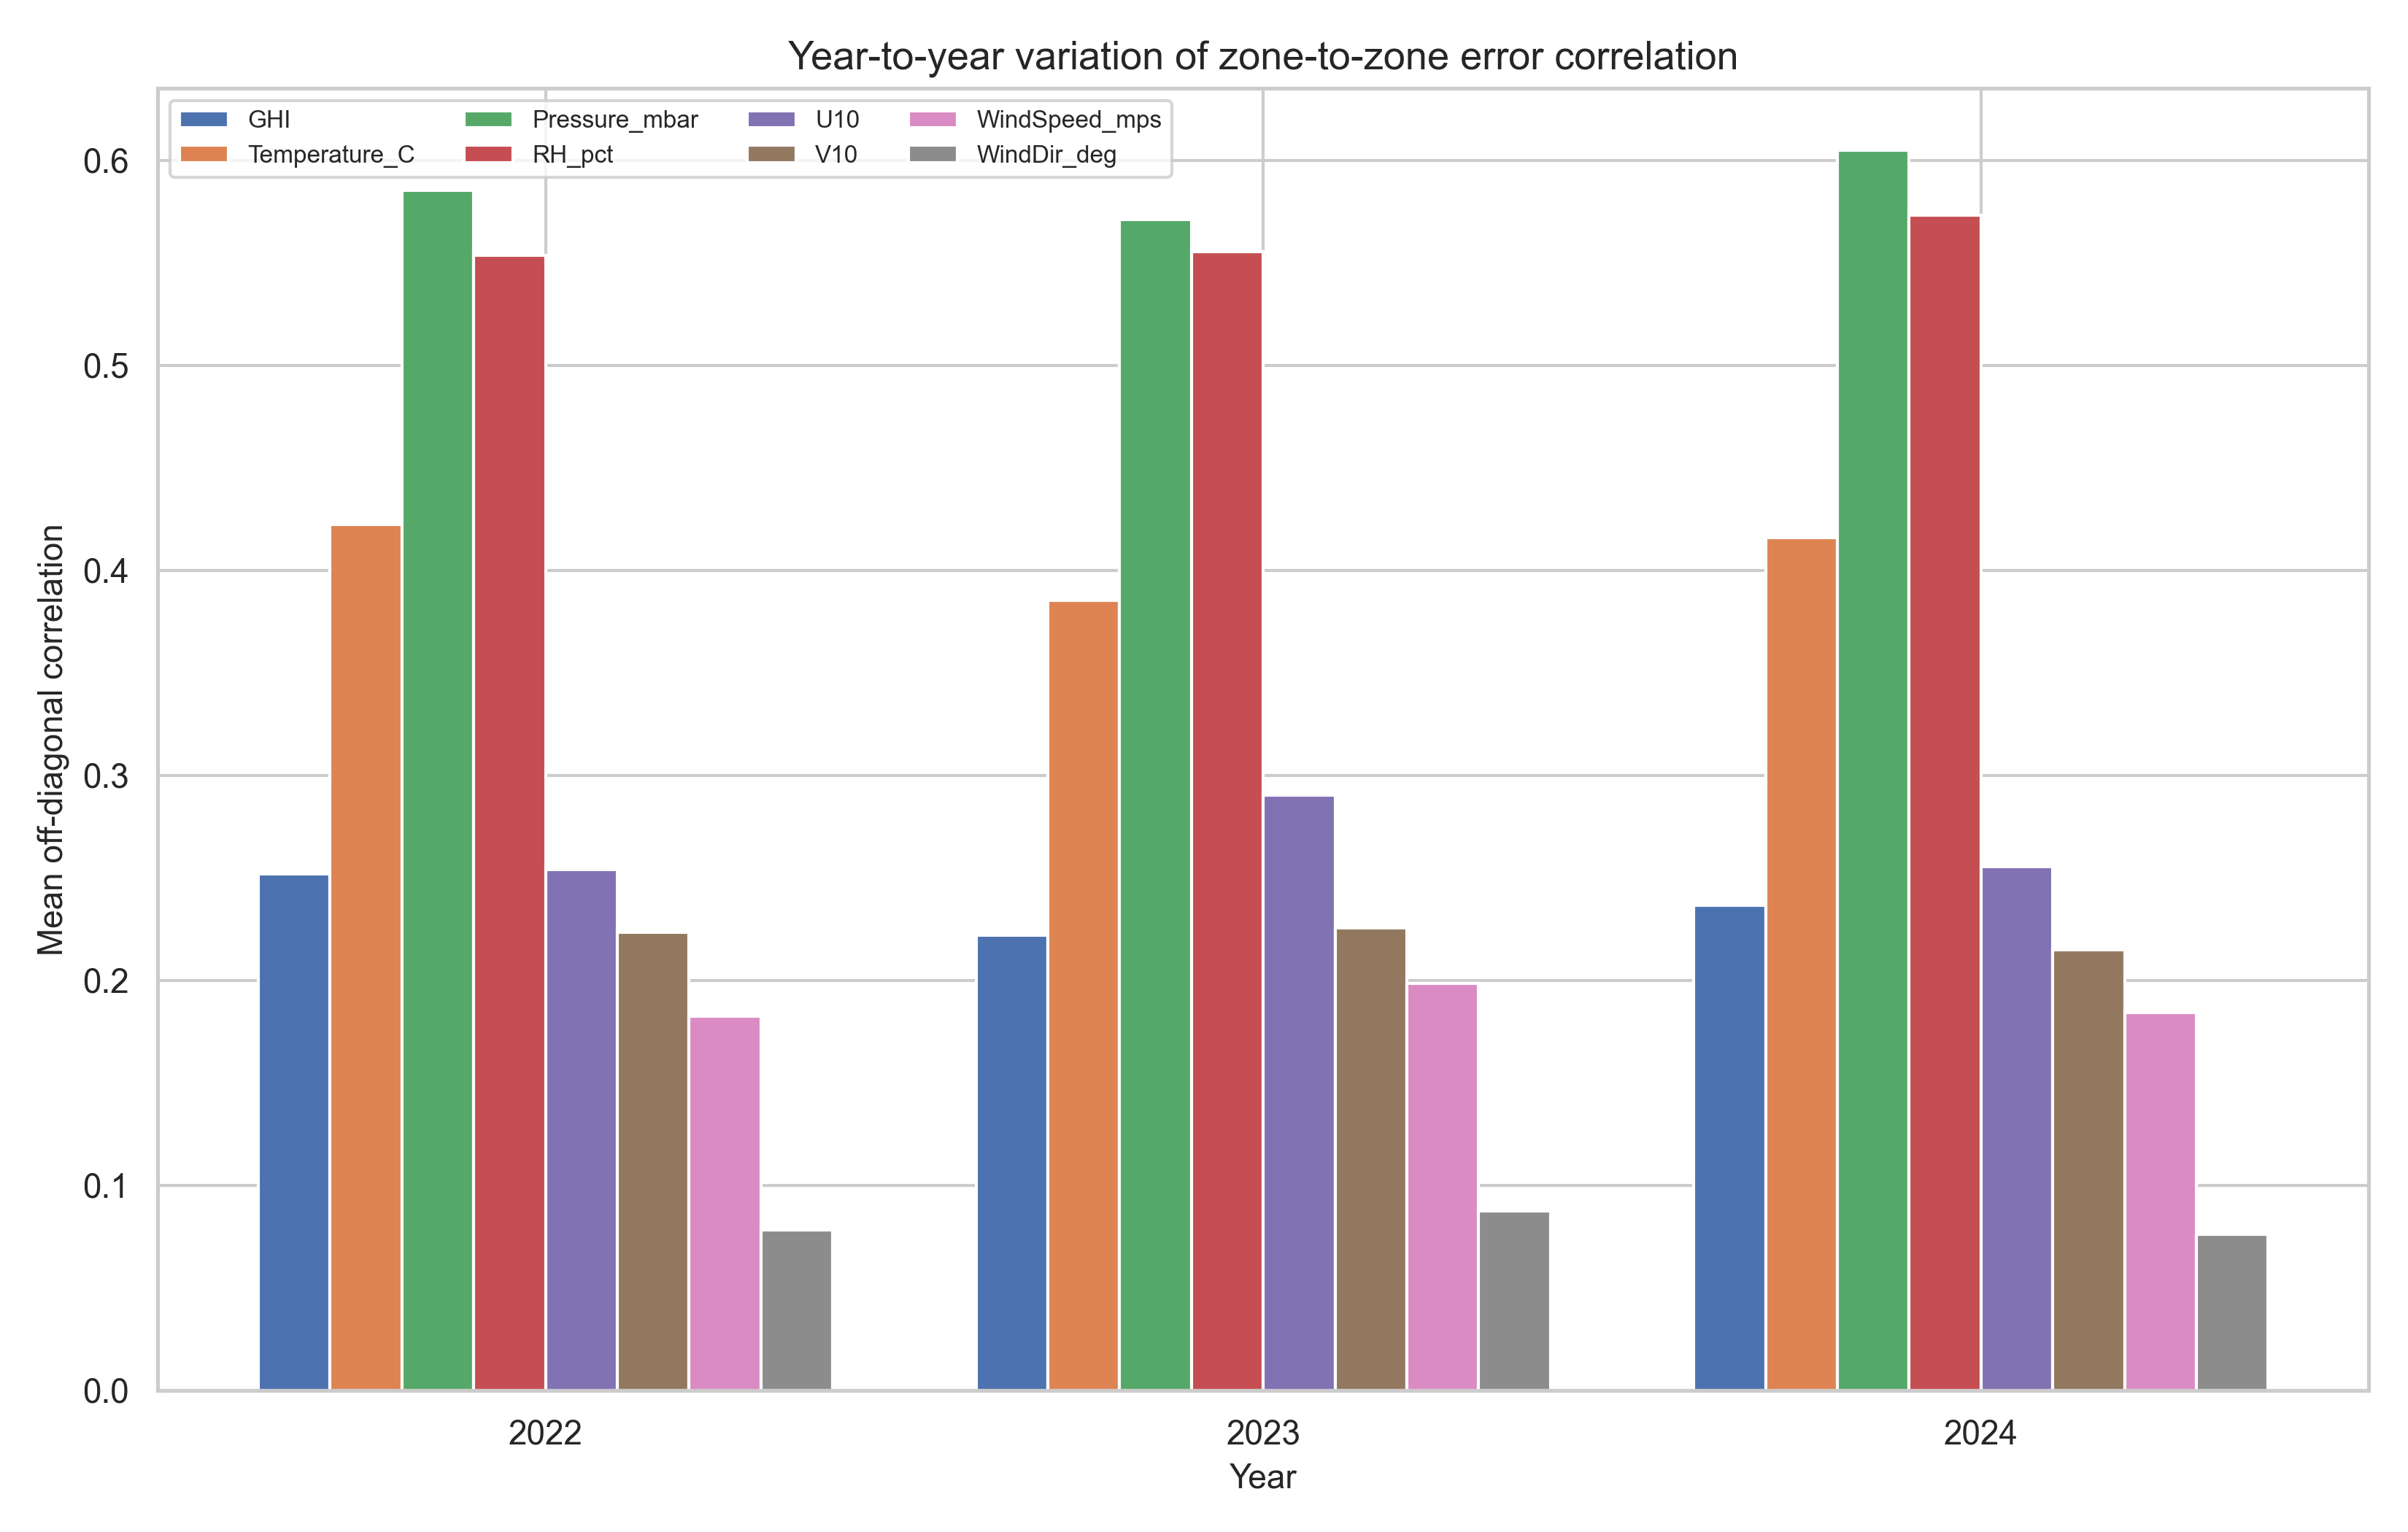
\includegraphics[width=\textwidth]{figures/Q9/yearly_zone_correlation.png}
  \caption{Year-to-year variation of zone-to-zone forecast-error correlation. Each bar is the
  mean off-diagonal Pearson~$r$ of the $9\times 9$ zone-to-zone correlation matrix (zone-mean
  signed error, all lead times pooled) for one variable in one year. The bars are nearly
  identical across 2022, 2023, and 2024---pressure and RH stay the most cross-zone coherent
  ($r\approx0.55$--$0.61$), temperature is intermediate ($\approx0.4$), GHI and the wind
  components sit near $0.2$--$0.3$, and wind direction is a flat low floor ($\approx0.08$)---so
  the spatial-correlation structure of the error is essentially stable from year to year. Models
  or portfolio strategies calibrated on one year therefore carry over to the next. (GHI uses
  daytime samples only, $\text{GHI}_{\text{act}}>\SI{5}{W/m^2}$.)}
  \label{fig:yearcorr}
\end{figure}

\subsection{Portfolio takeaway}

Cross-zone error diversification is best in \textbf{summer} (shortest decorrelation lengths,
lowest GHI coherence), weakest in autumn/winter, and stable from year to year. Pressure error
never diversifies away in any stratum.

% ======================================================================
\section{Discussion}\label{sec:discussion}
% ======================================================================

PLACEHOLDER: Two practical conclusions emerge for operating a solar portfolio under forecast uncertainty.

First, \emph{the temporal structure of error is partly correctable.} The dominant pattern in
error growth is a diurnal cycle (statistically significant for GHI, RH, U10, and wind direction),
not monotonic horizon-driven drift. A harmonic bias correction keyed to time of day would remove
a meaningful component of error without any change to the underlying forecast model. The fixed
\texttt{06z} initialization limits how cleanly we can separate genuine lead-time growth from the
diurnal cycle; forecasts from multiple initialization times would be required to fully resolve
that confound.

Second, \emph{spatial diversification is real but variable-specific and season-specific.}
Cloud-driven irradiance error---the component that matters most for solar output---decorrelates
over the shortest distances, so a geographically spread fleet genuinely smooths it, especially in
summer. Synoptic fields such as surface pressure stay correlated across the entire PJM footprint
and cannot be diversified away. Any portfolio-level uncertainty model should therefore treat these
variable classes differently rather than assuming a single fleet-wide correlation.

% ======================================================================
\section{Conclusion}\label{sec:conclusion}
% ======================================================================

PLACEHOLDER: Across the PJM solar fleet, forecast error grows with lead time mainly through a diurnal cycle
rather than directional bias drift, and its spatial coherence ranges from synoptic-scale
(pressure: $L \approx \SI{445}{km}$) to highly local (GHI: $L \approx \SI{134}{km}$). That
coherence contracts in summer and follows a diurnal rhythm but is stable year to year. The
combined picture tells an operator \emph{when} forecast error is most uncertain (mid-horizon,
solar-noon leads) and \emph{where} aggregating sites actually reduces it (irradiance and wind
direction, especially in summer)---the quantitative basis for both bias correction and
portfolio-level uncertainty estimation.

% ======================================================================
\section{Appendix}\label{sec:appendix}
% ======================================================================

Collection of our cool graphs


% --- Data and Methods - Graphs ---

\subsection{Q1 — Descriptive Statistics}

\begin{figure}[H]
  \centering
  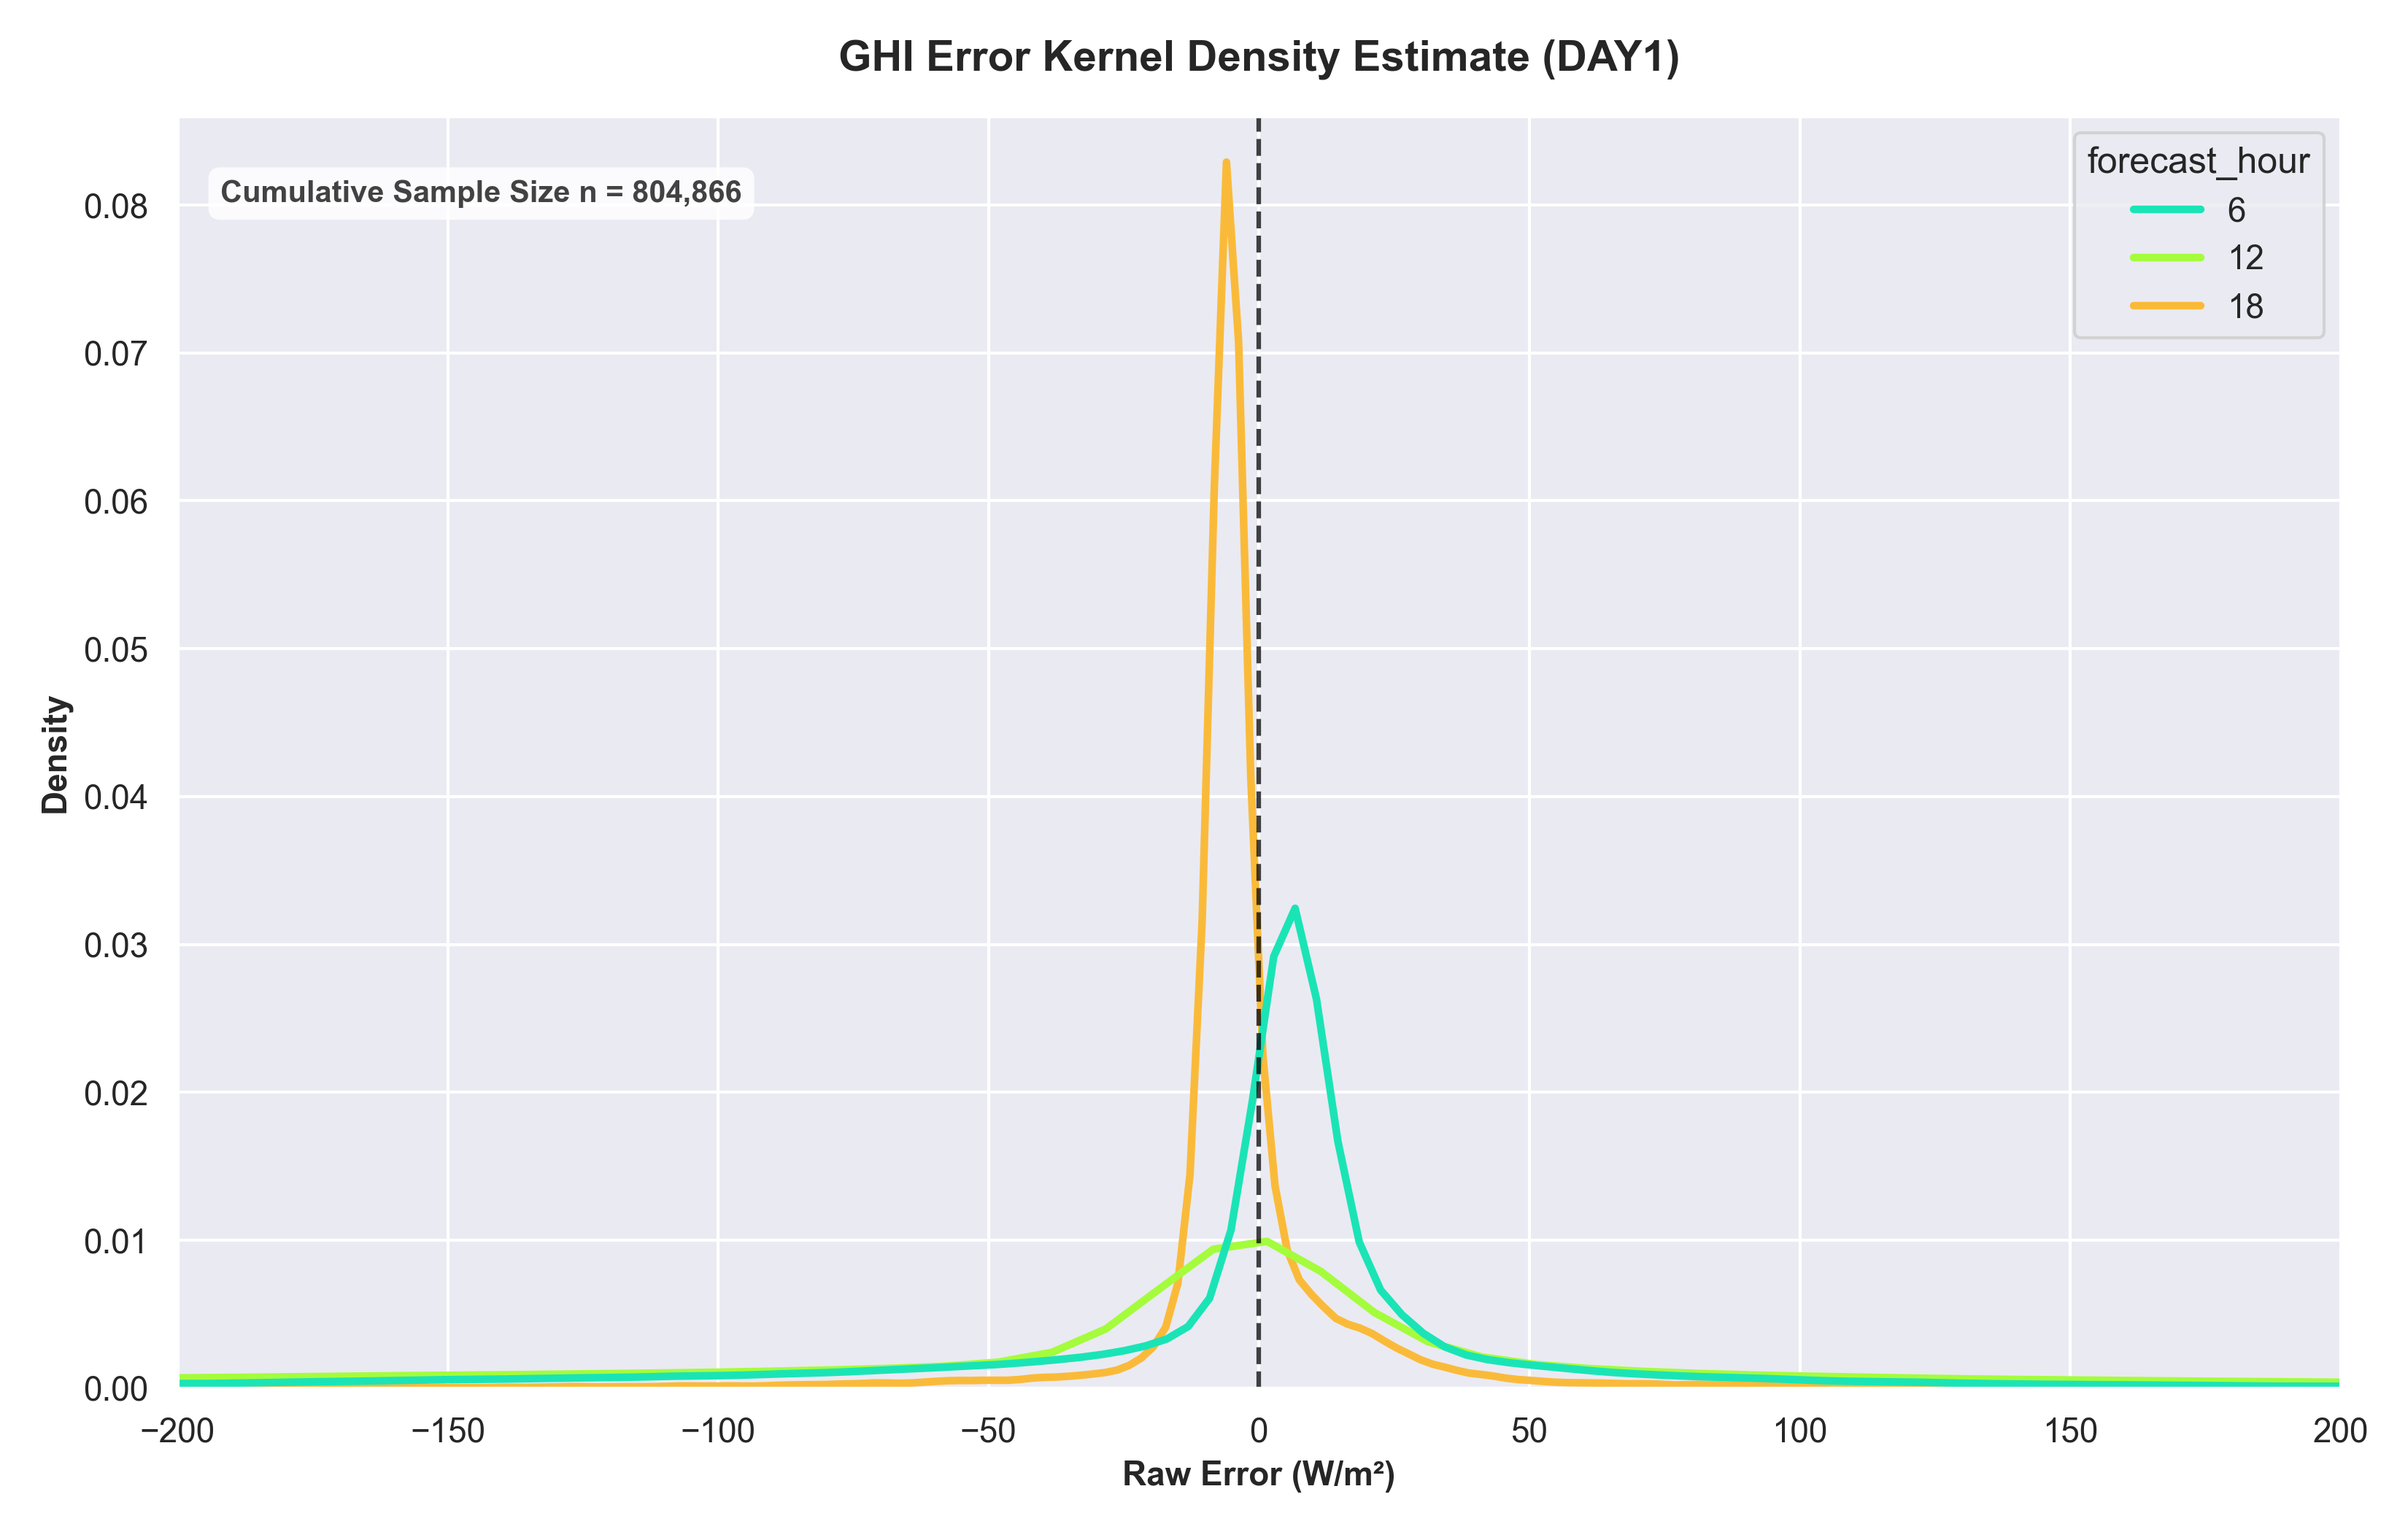
\includegraphics[width=0.49\textwidth]{figures/KDE_GRAPHS_RAW/ghi_kde_day1.png}\hfill
  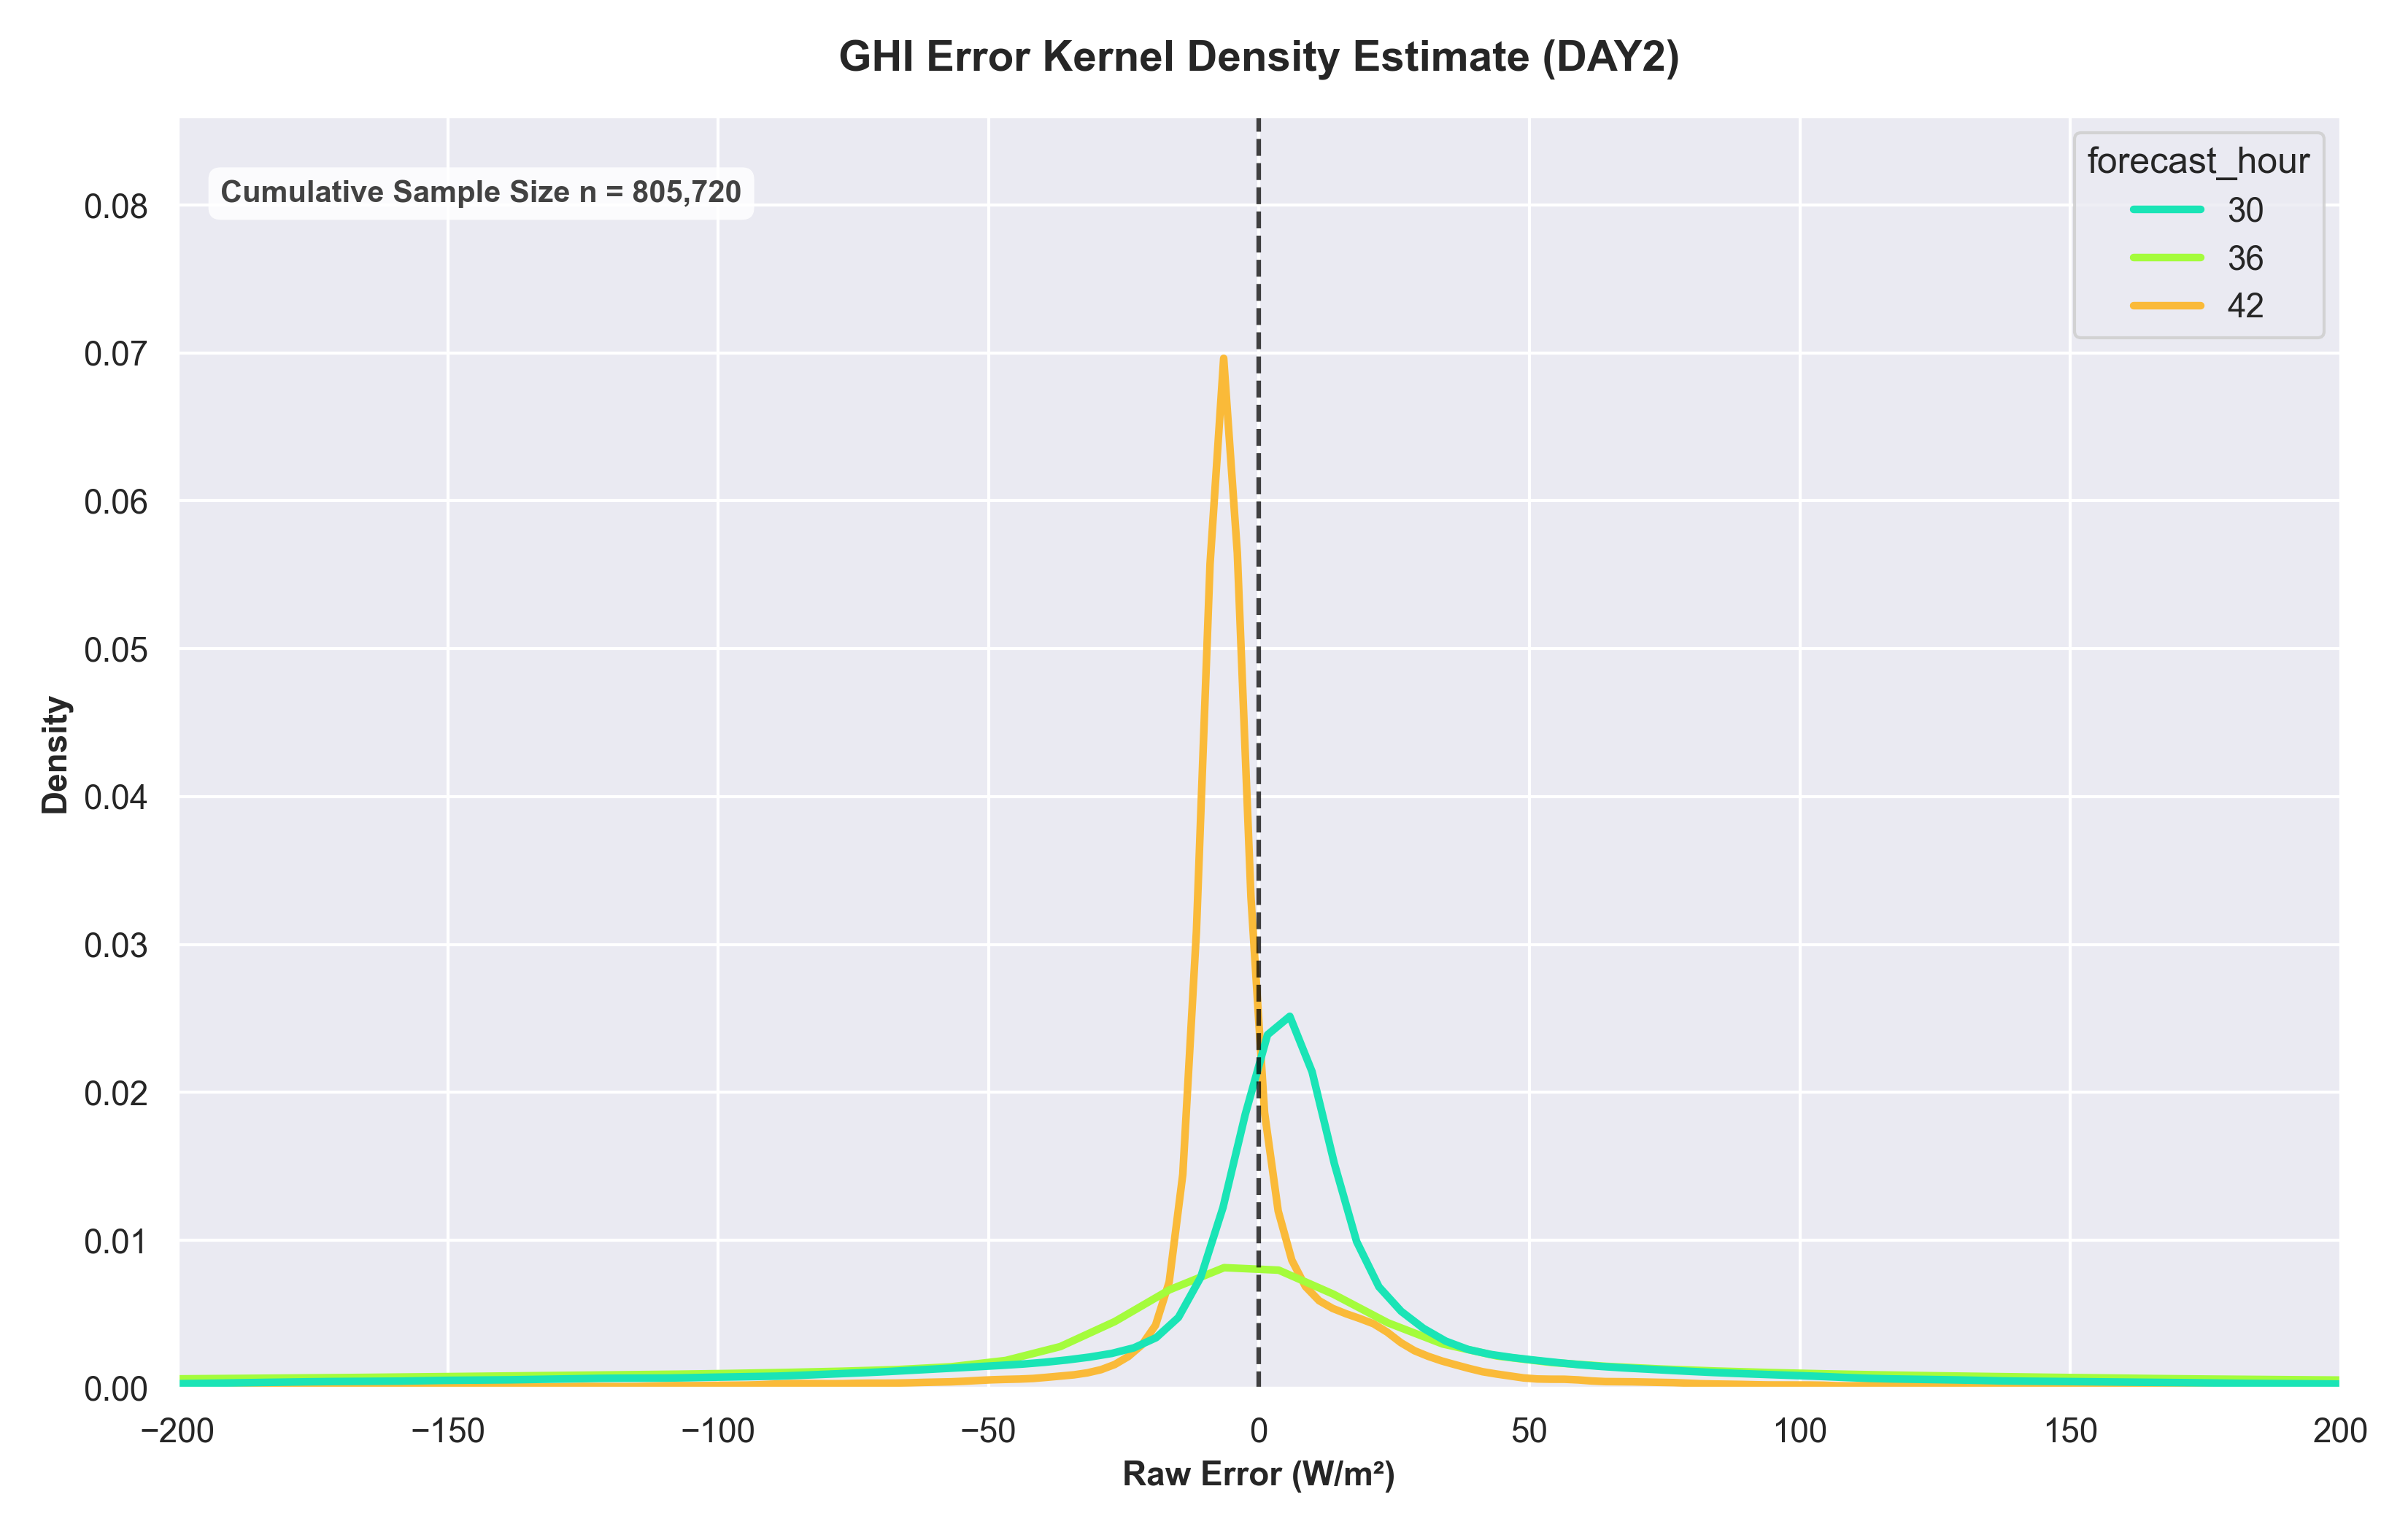
\includegraphics[width=0.49\textwidth]{figures/KDE_GRAPHS_RAW/ghi_kde_day2.png}
  \caption{Kernel Density Estimation (KDE) of Global Horizontal Irradiance (GHI) forecast errors for Day 1 (left) and Day 2 (right).}
  \label{fig:kde_ghi}
\end{figure}

\begin{figure}[H]
  \centering
  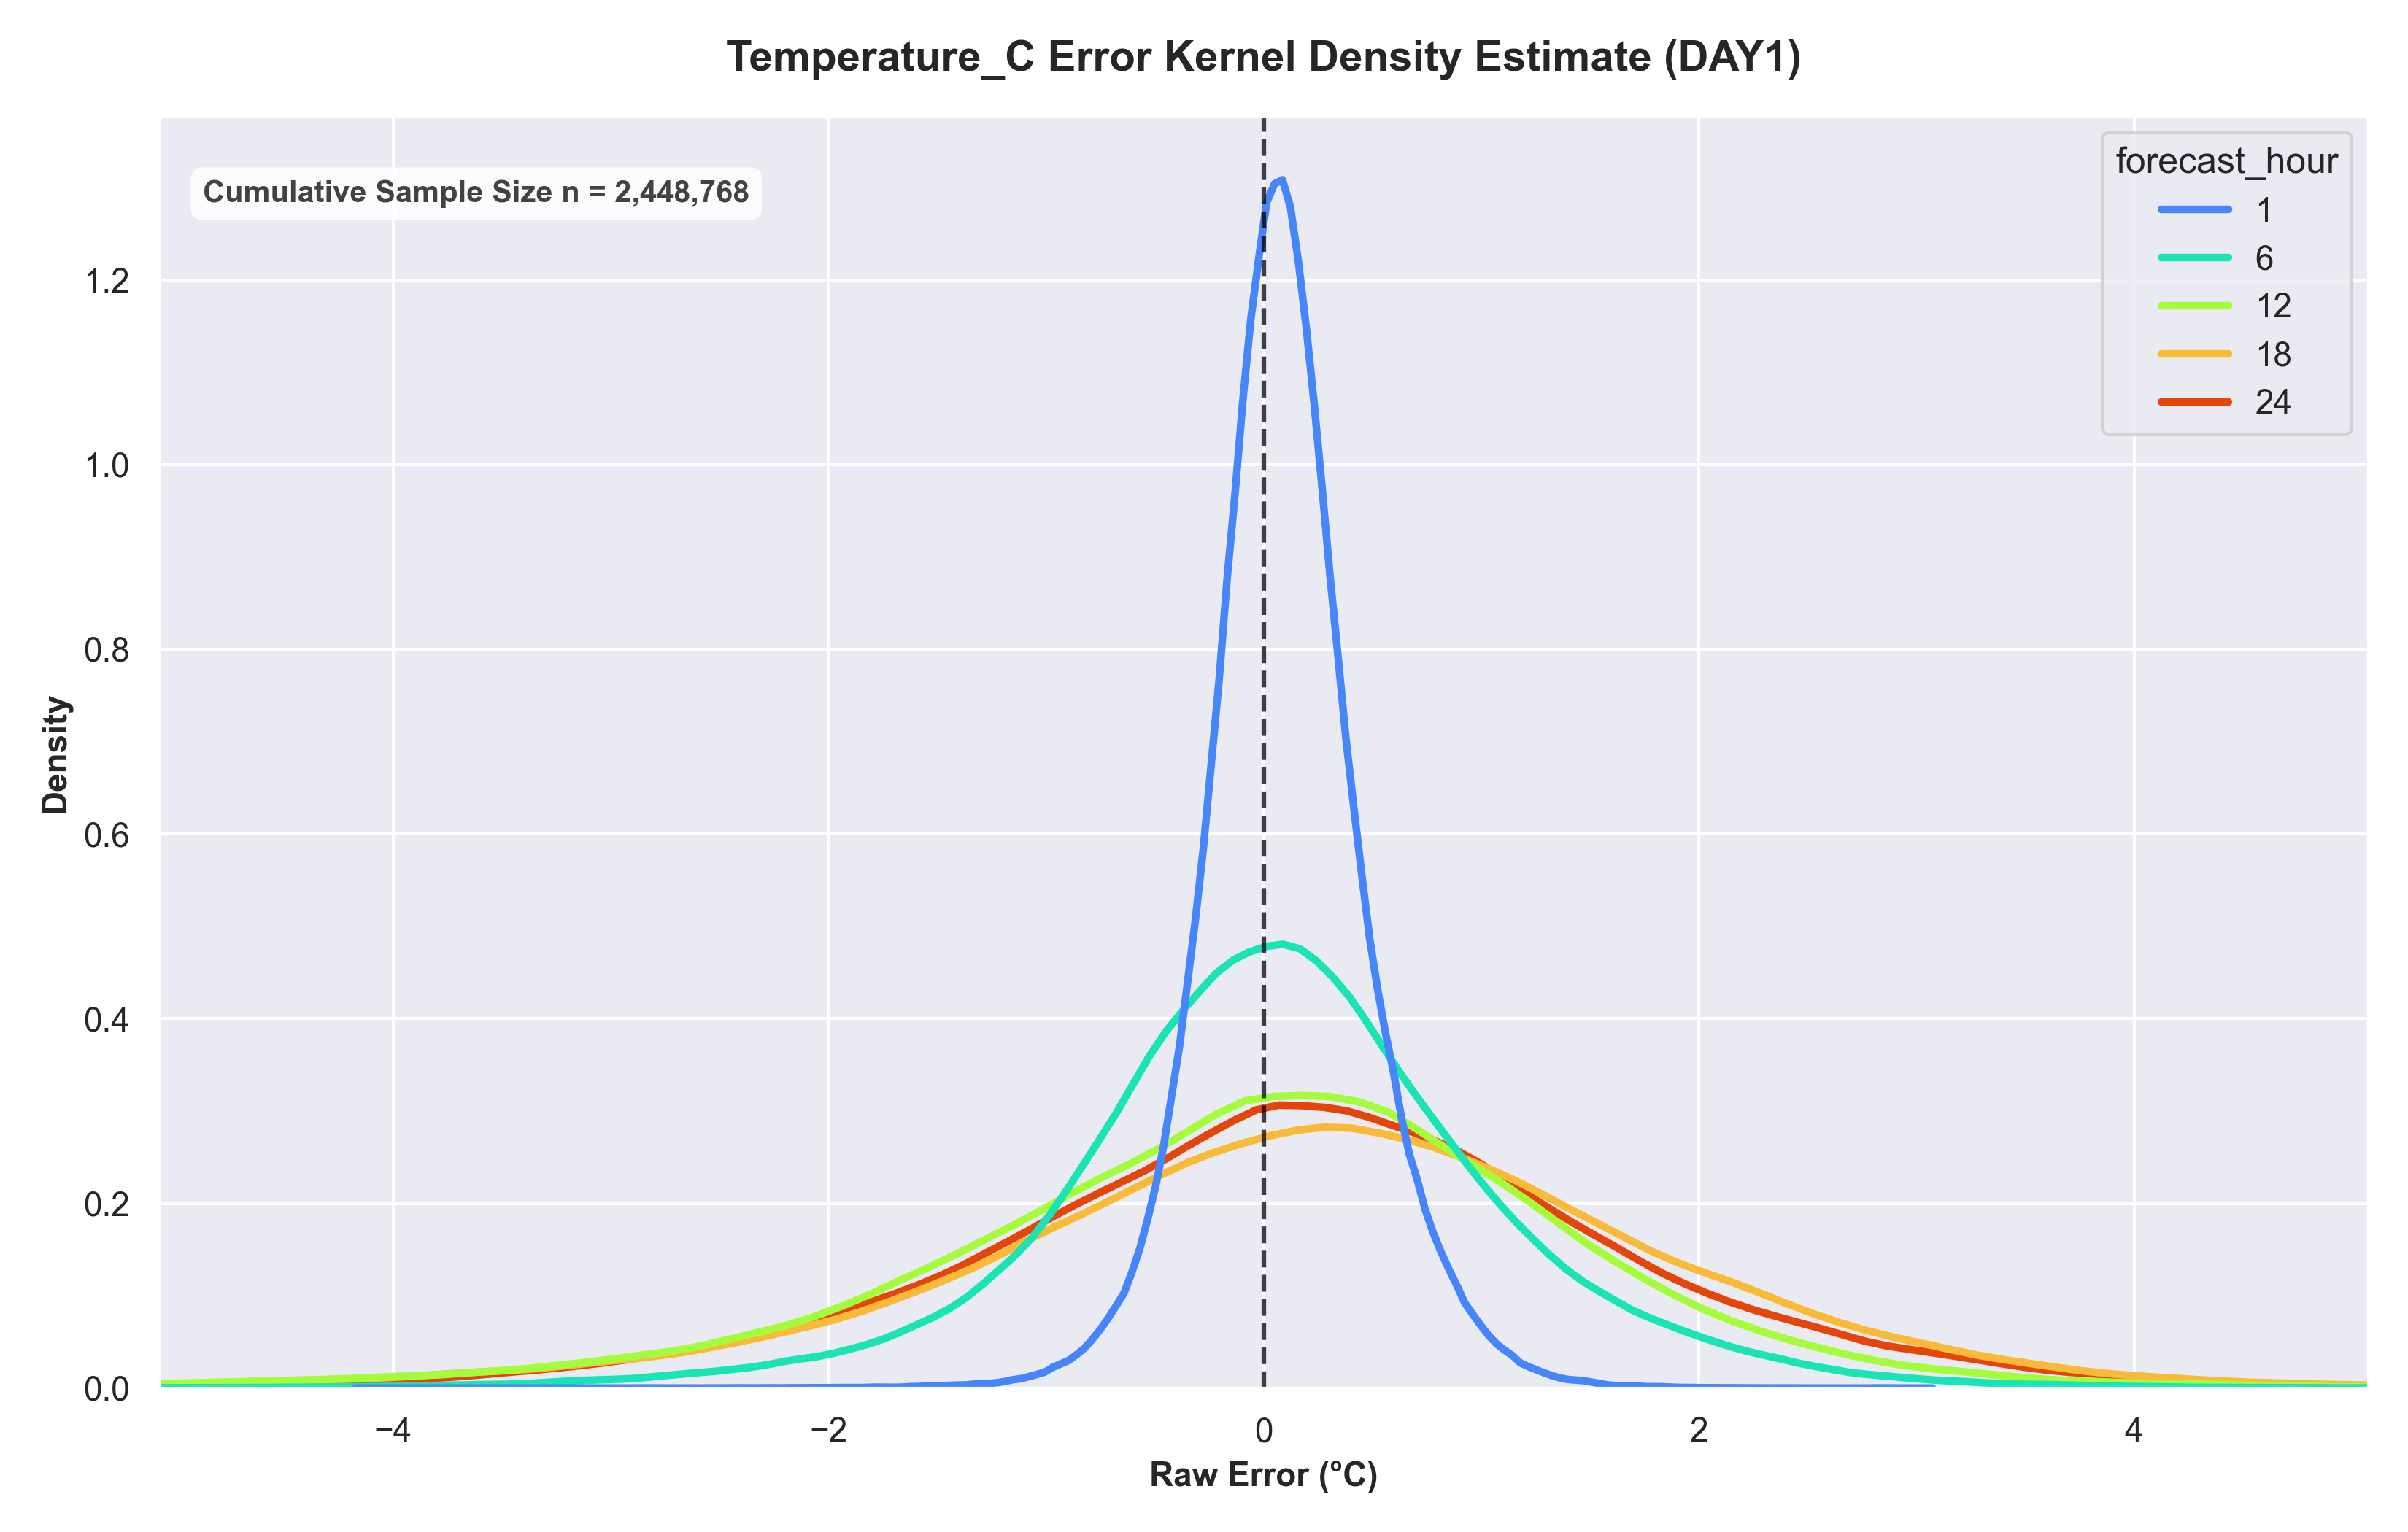
\includegraphics[width=0.49\textwidth]{figures/KDE_GRAPHS_RAW/temperature_c_kde_day1.png}\hfill
  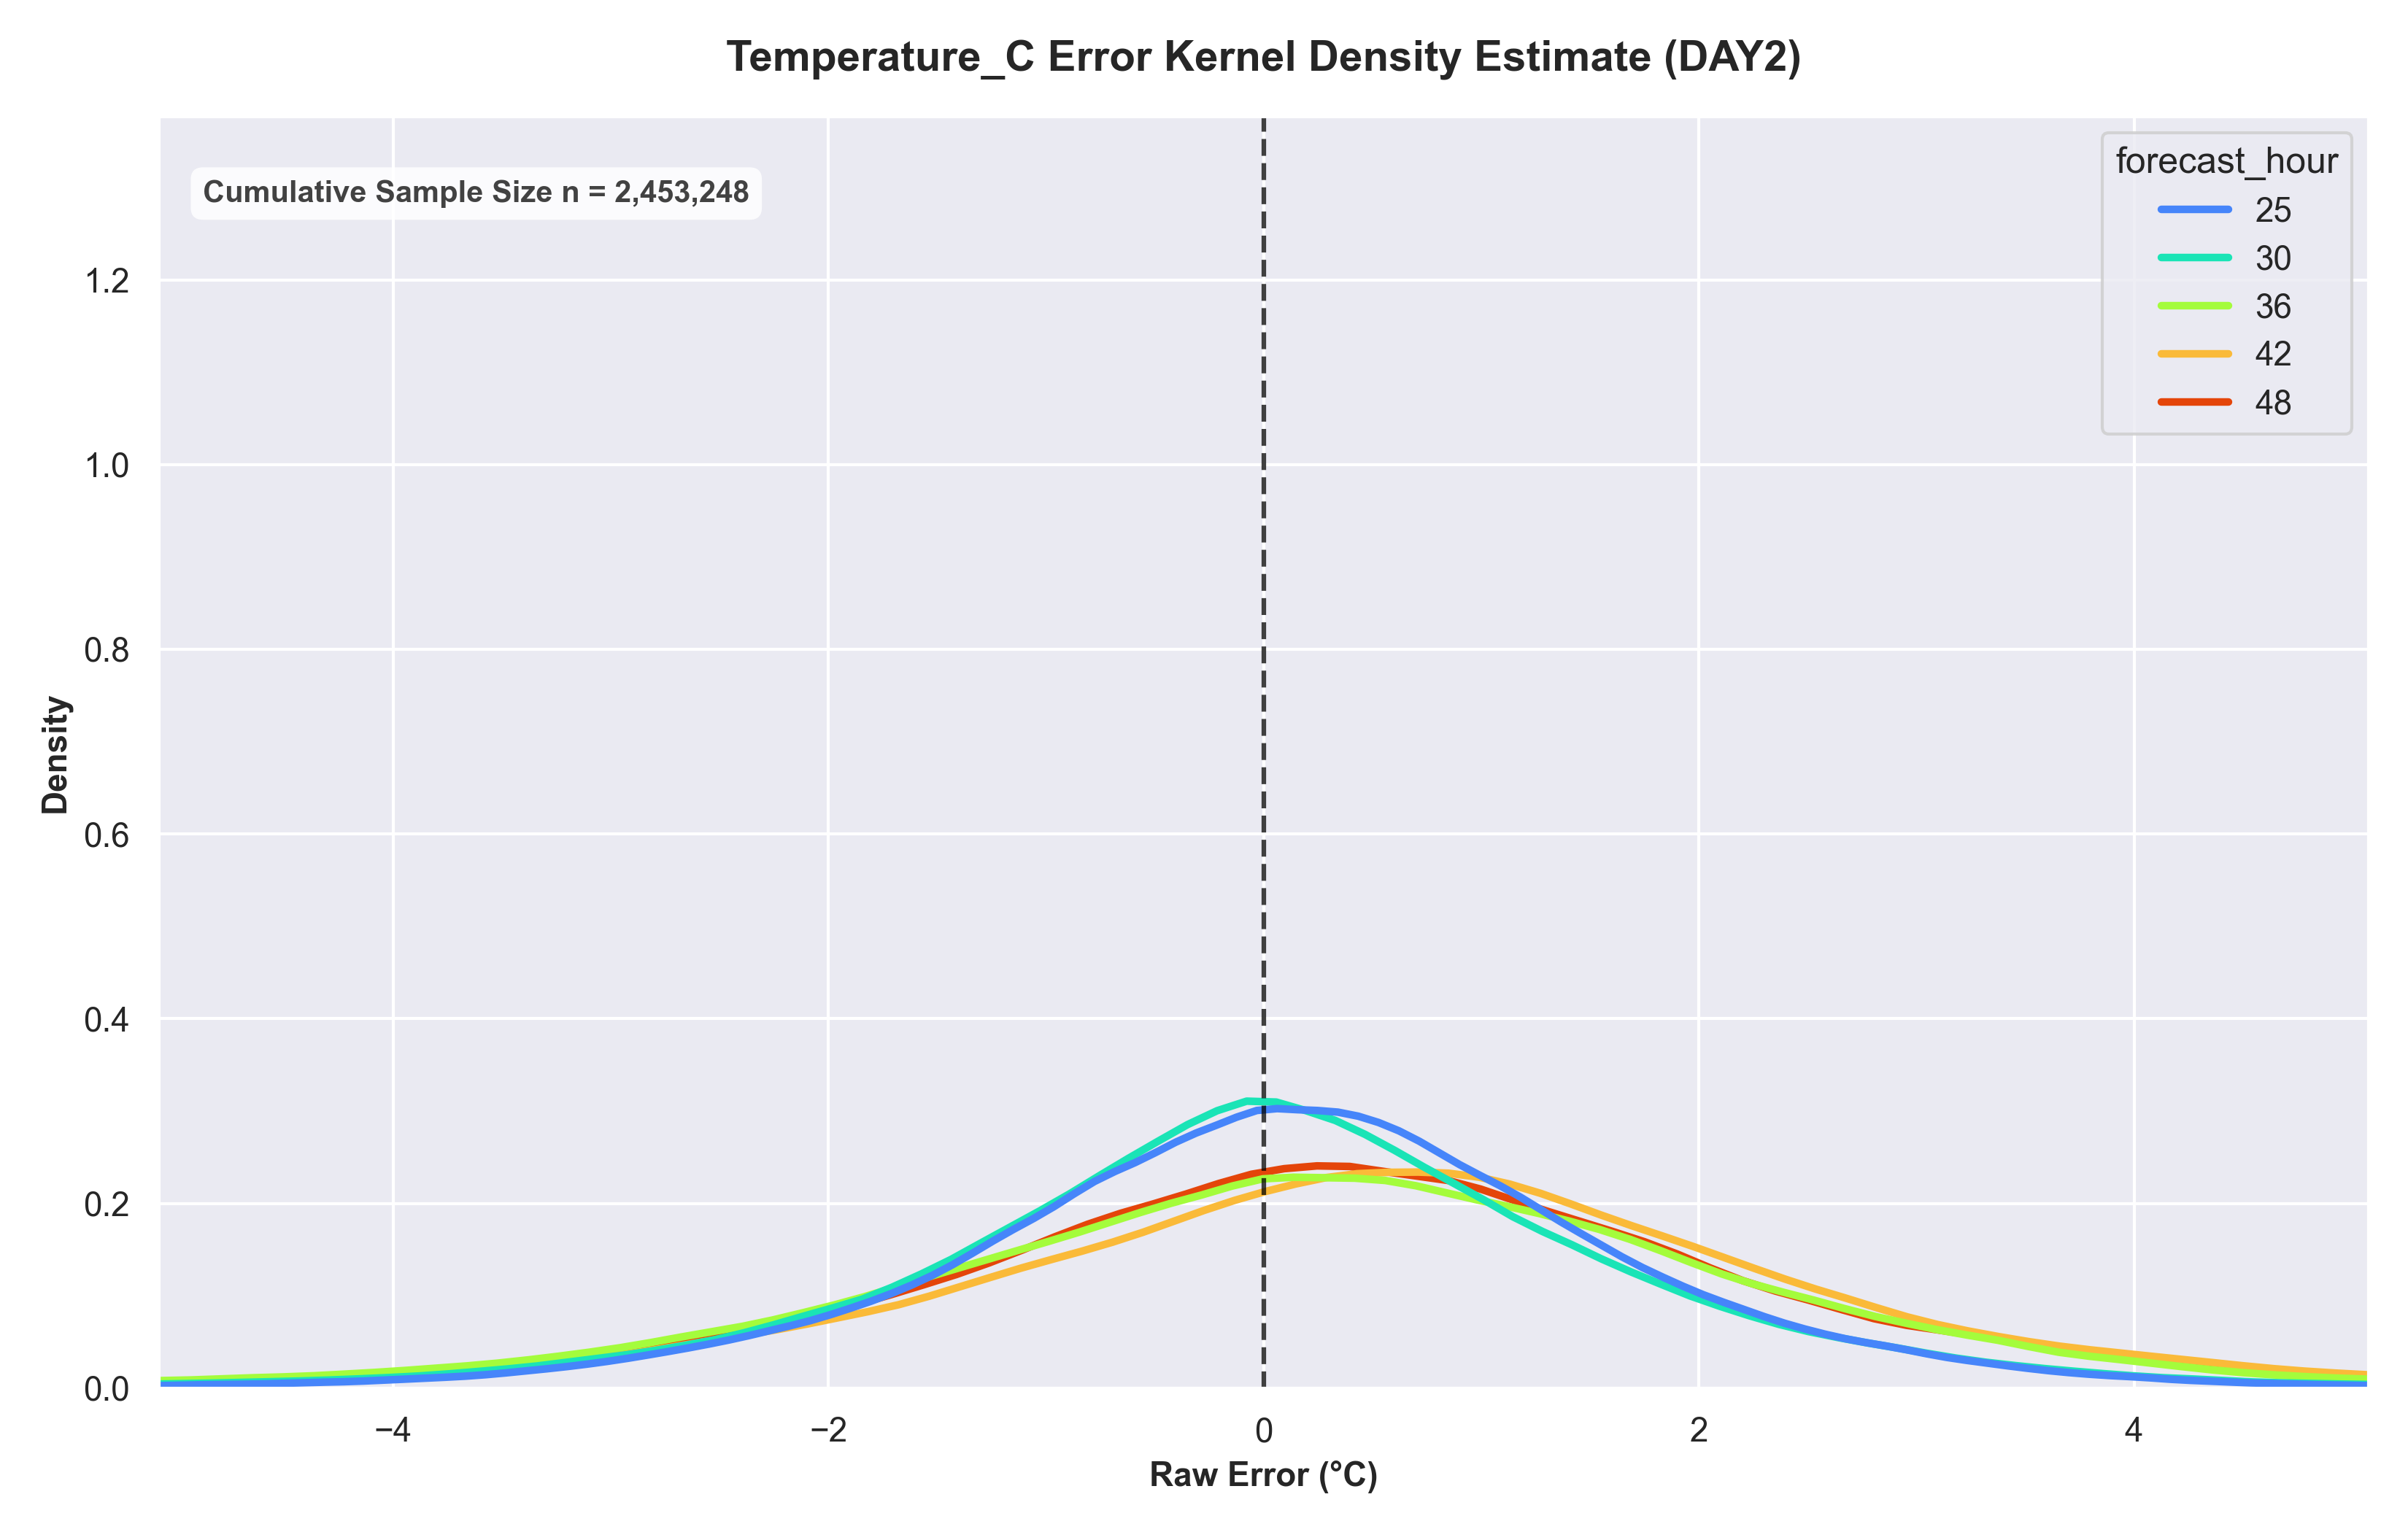
\includegraphics[width=0.49\textwidth]{figures/KDE_GRAPHS_RAW/temperature_c_kde_day2.png}
  \caption{Kernel Density Estimation (KDE) of Temperature forecast errors for Day 1 (left) and Day 2 (right).}
  \label{fig:kde_temp}
\end{figure}

\begin{figure}[H]
  \centering
  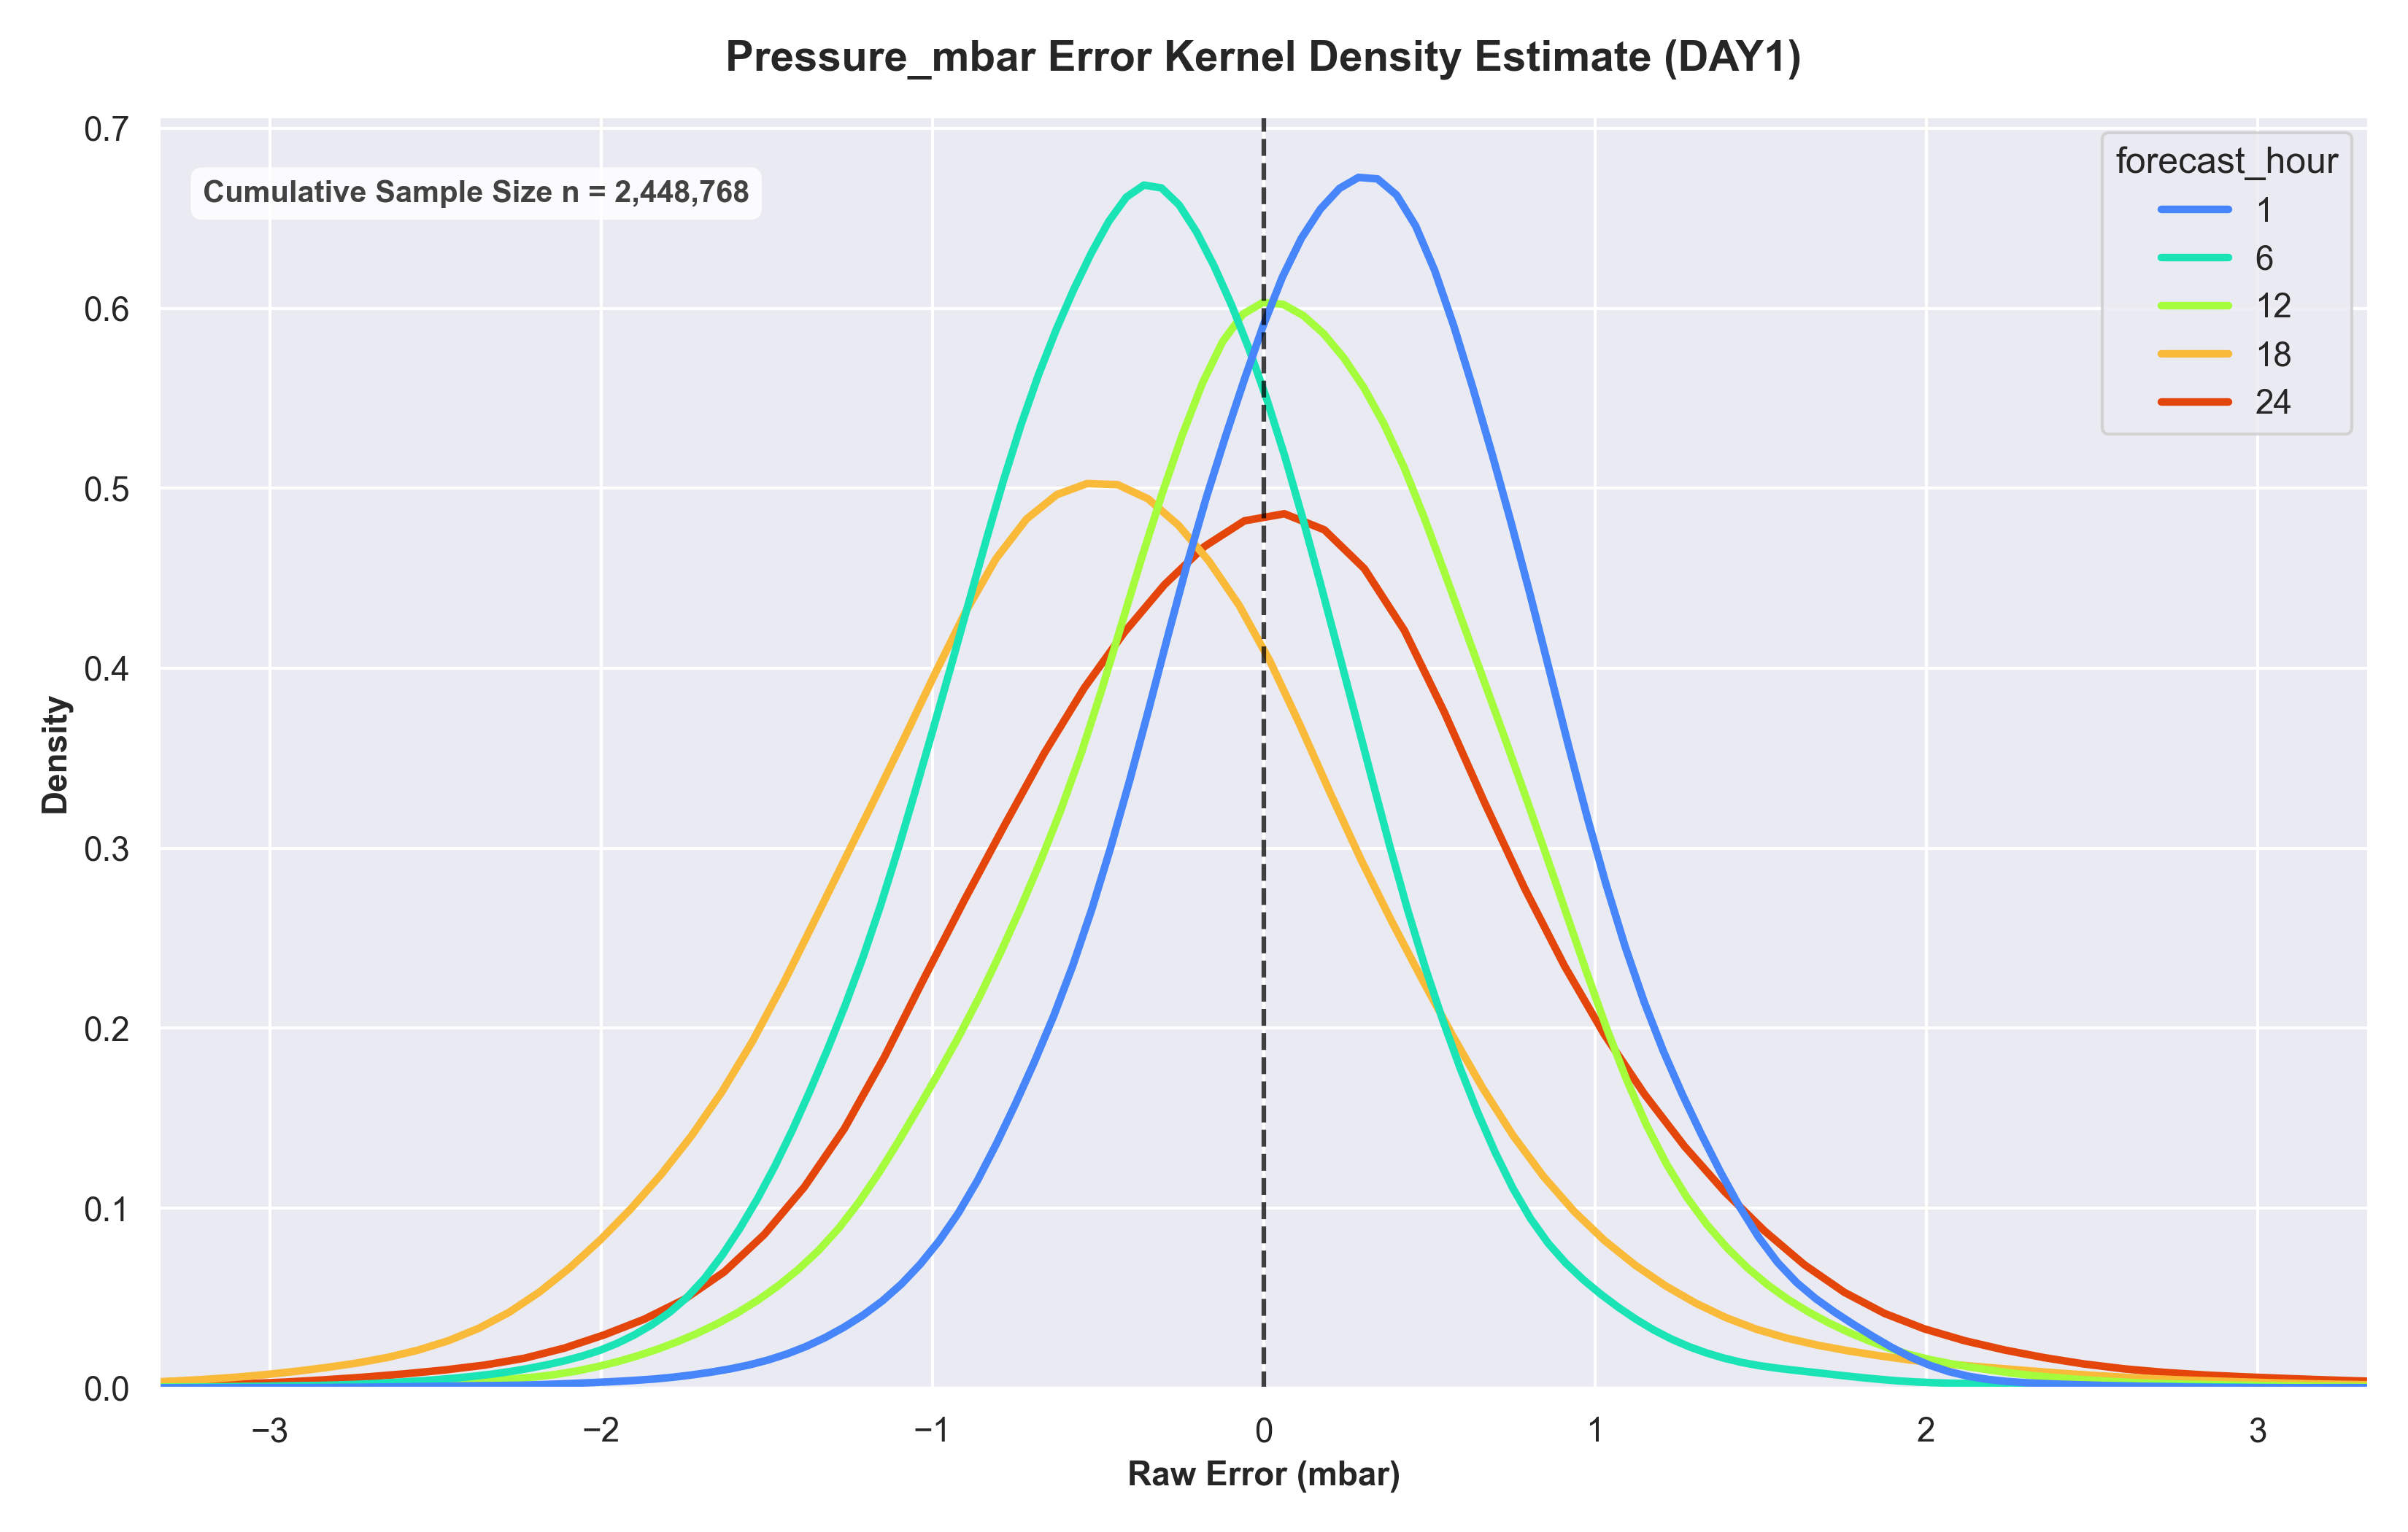
\includegraphics[width=0.49\textwidth]{figures/KDE_GRAPHS_RAW/pressure_mbar_kde_day1.png}\hfill
  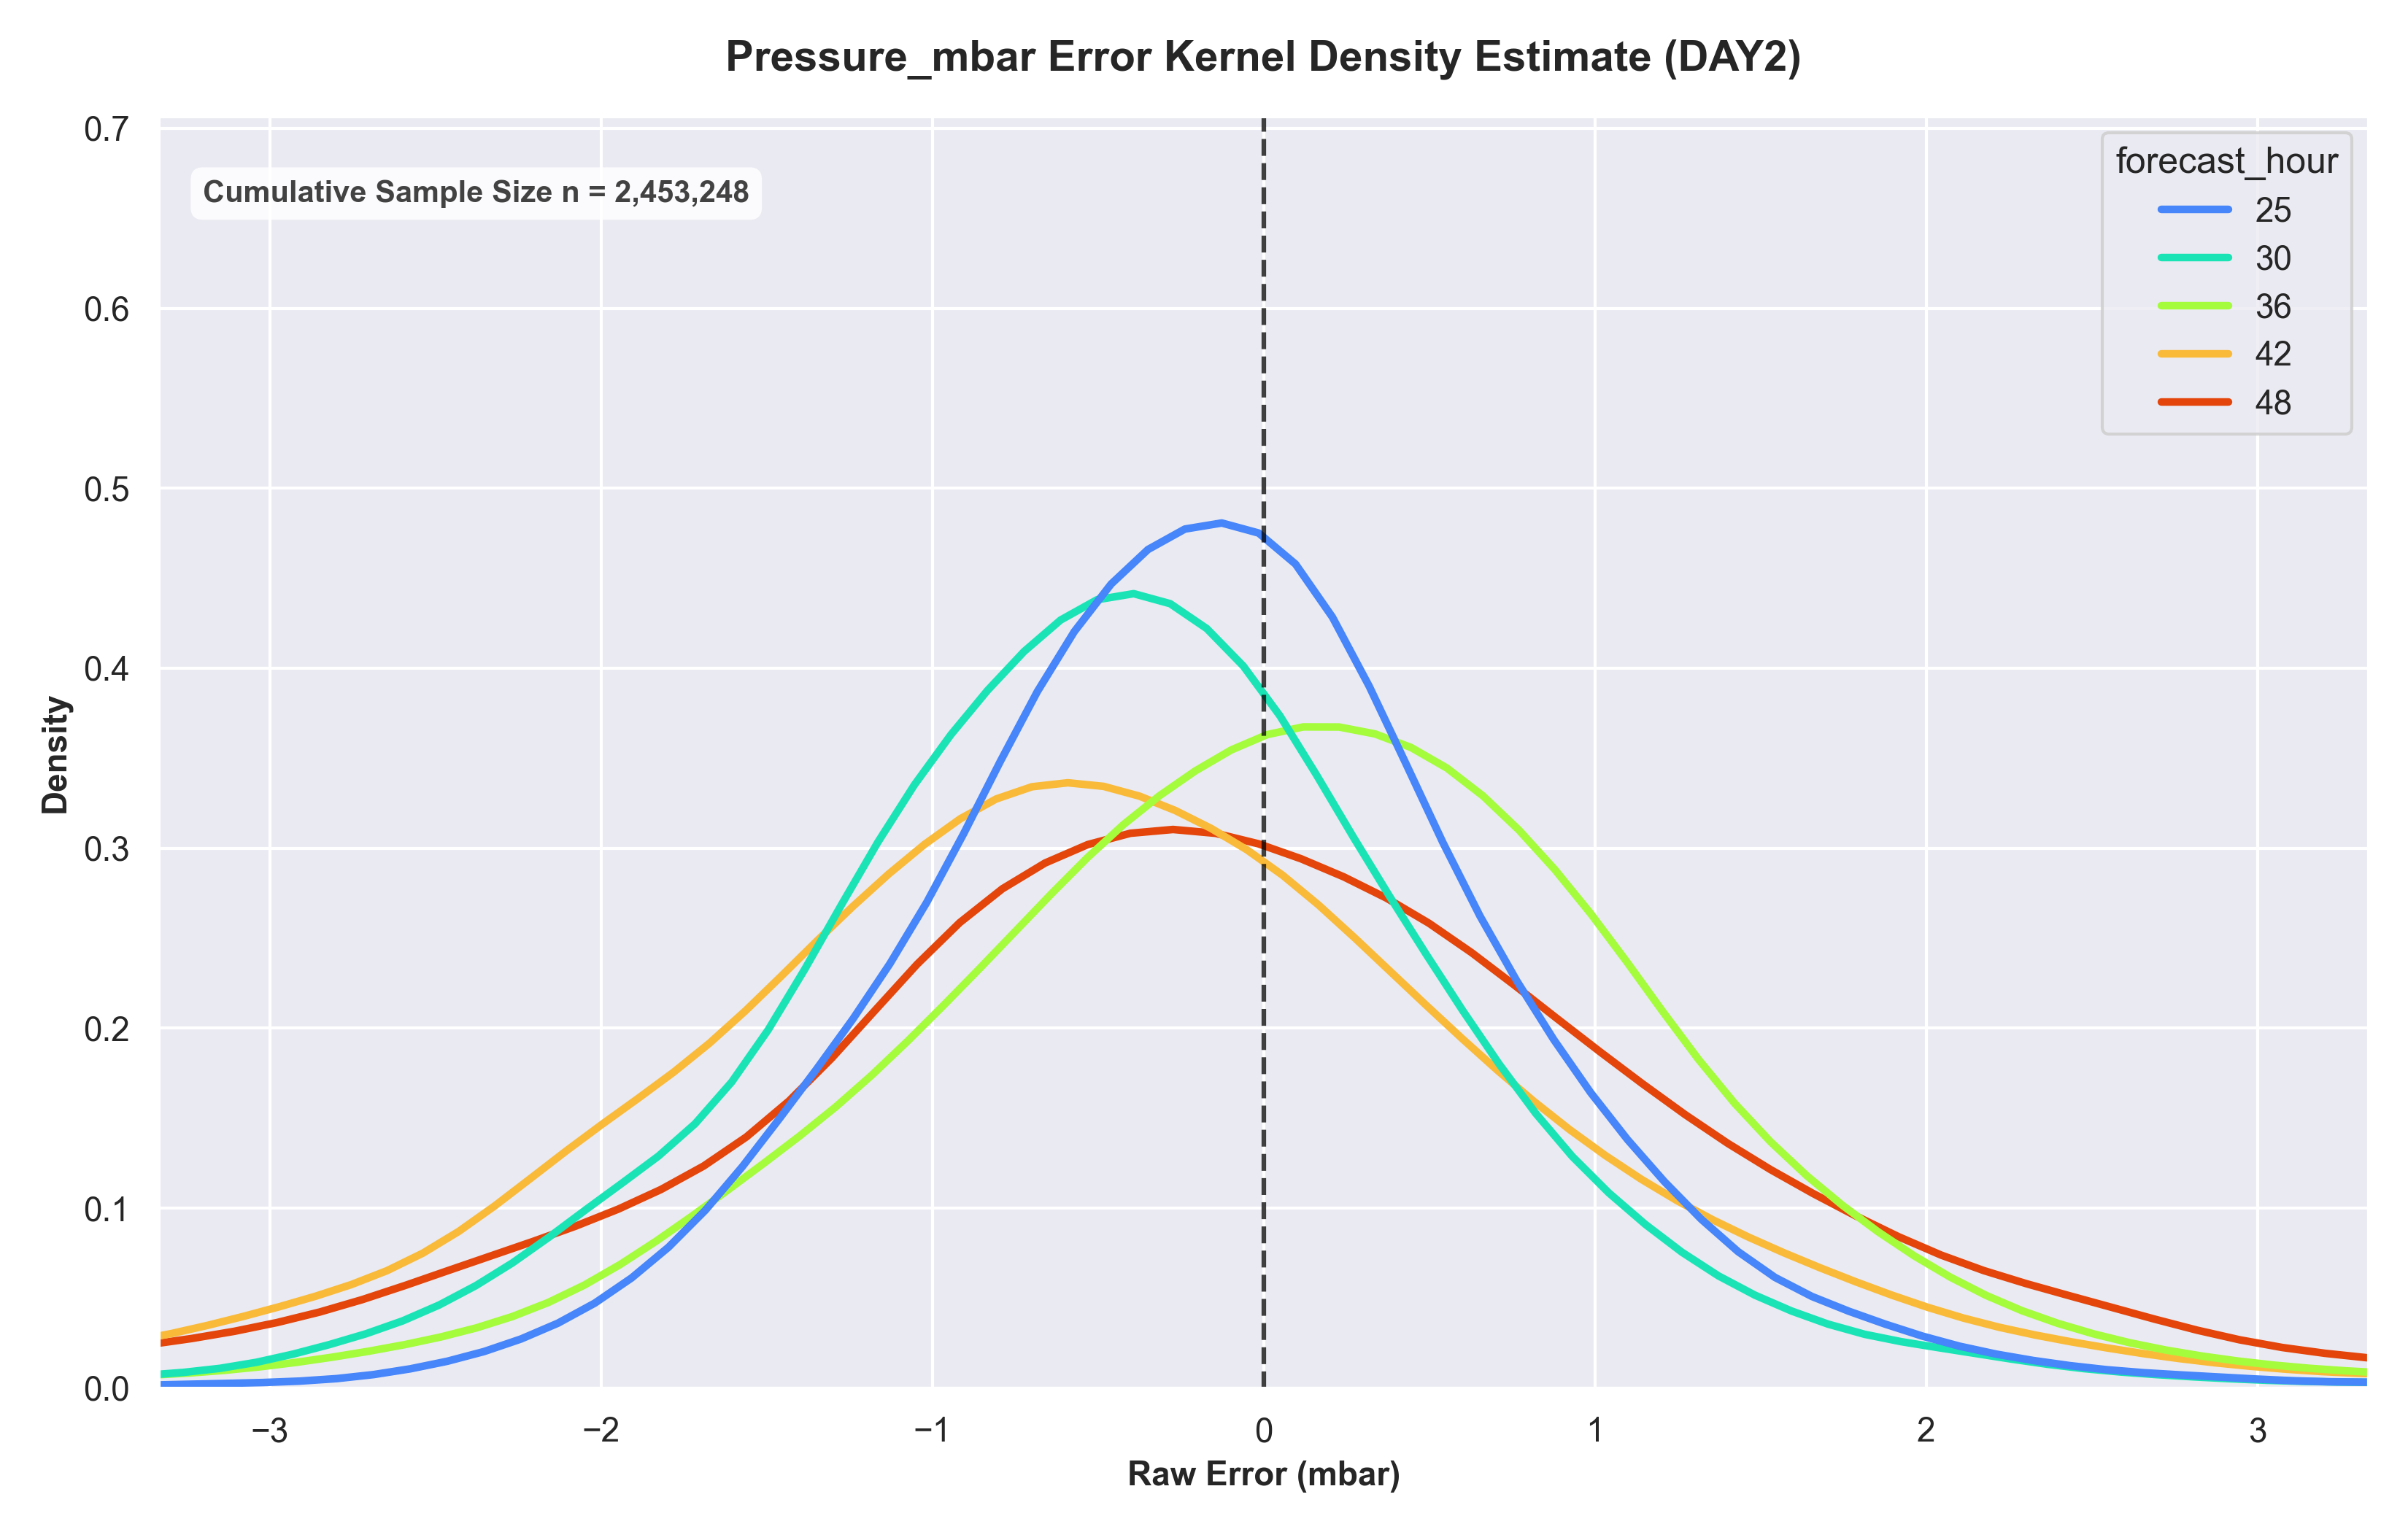
\includegraphics[width=0.49\textwidth]{figures/KDE_GRAPHS_RAW/pressure_mbar_kde_day2.png}
  \caption{Kernel Density Estimation (KDE) of Air Pressure forecast errors for Day 1 (left) and Day 2 (right).}
  \label{fig:kde_pressure}
\end{figure}

\begin{figure}[H]
  \centering
  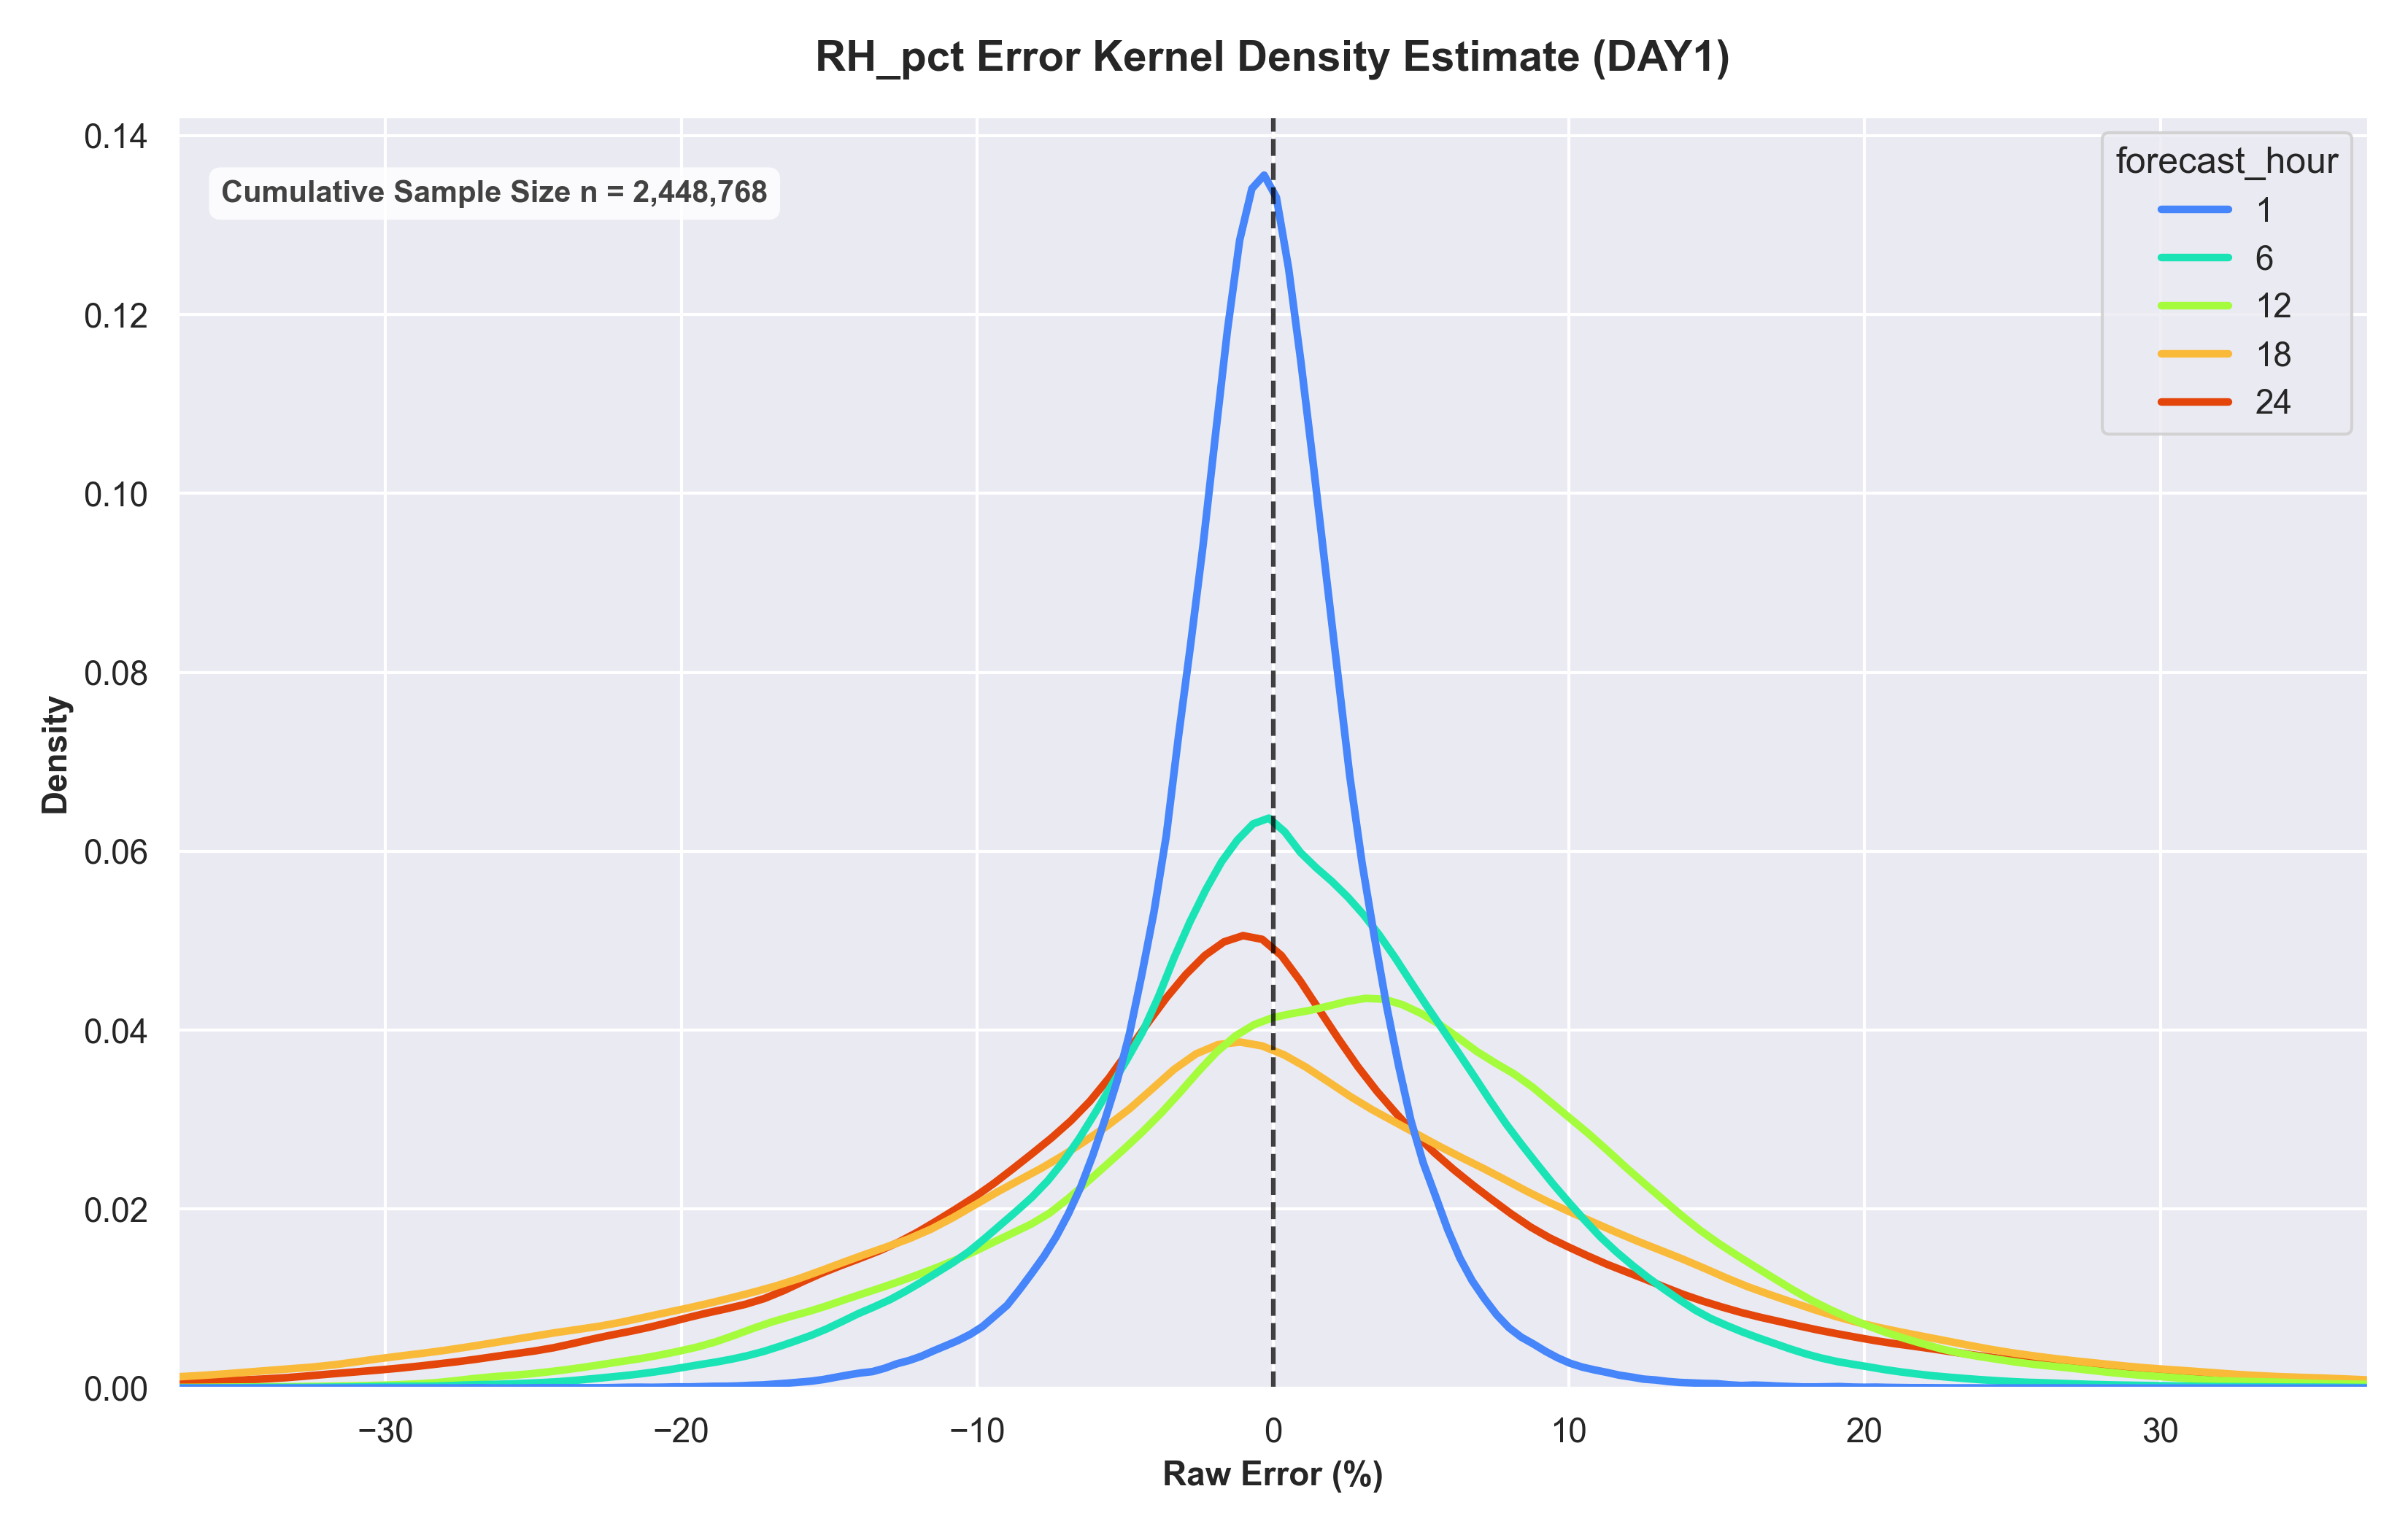
\includegraphics[width=0.49\textwidth]{figures/KDE_GRAPHS_RAW/rh_pct_kde_day1.png}\hfill
  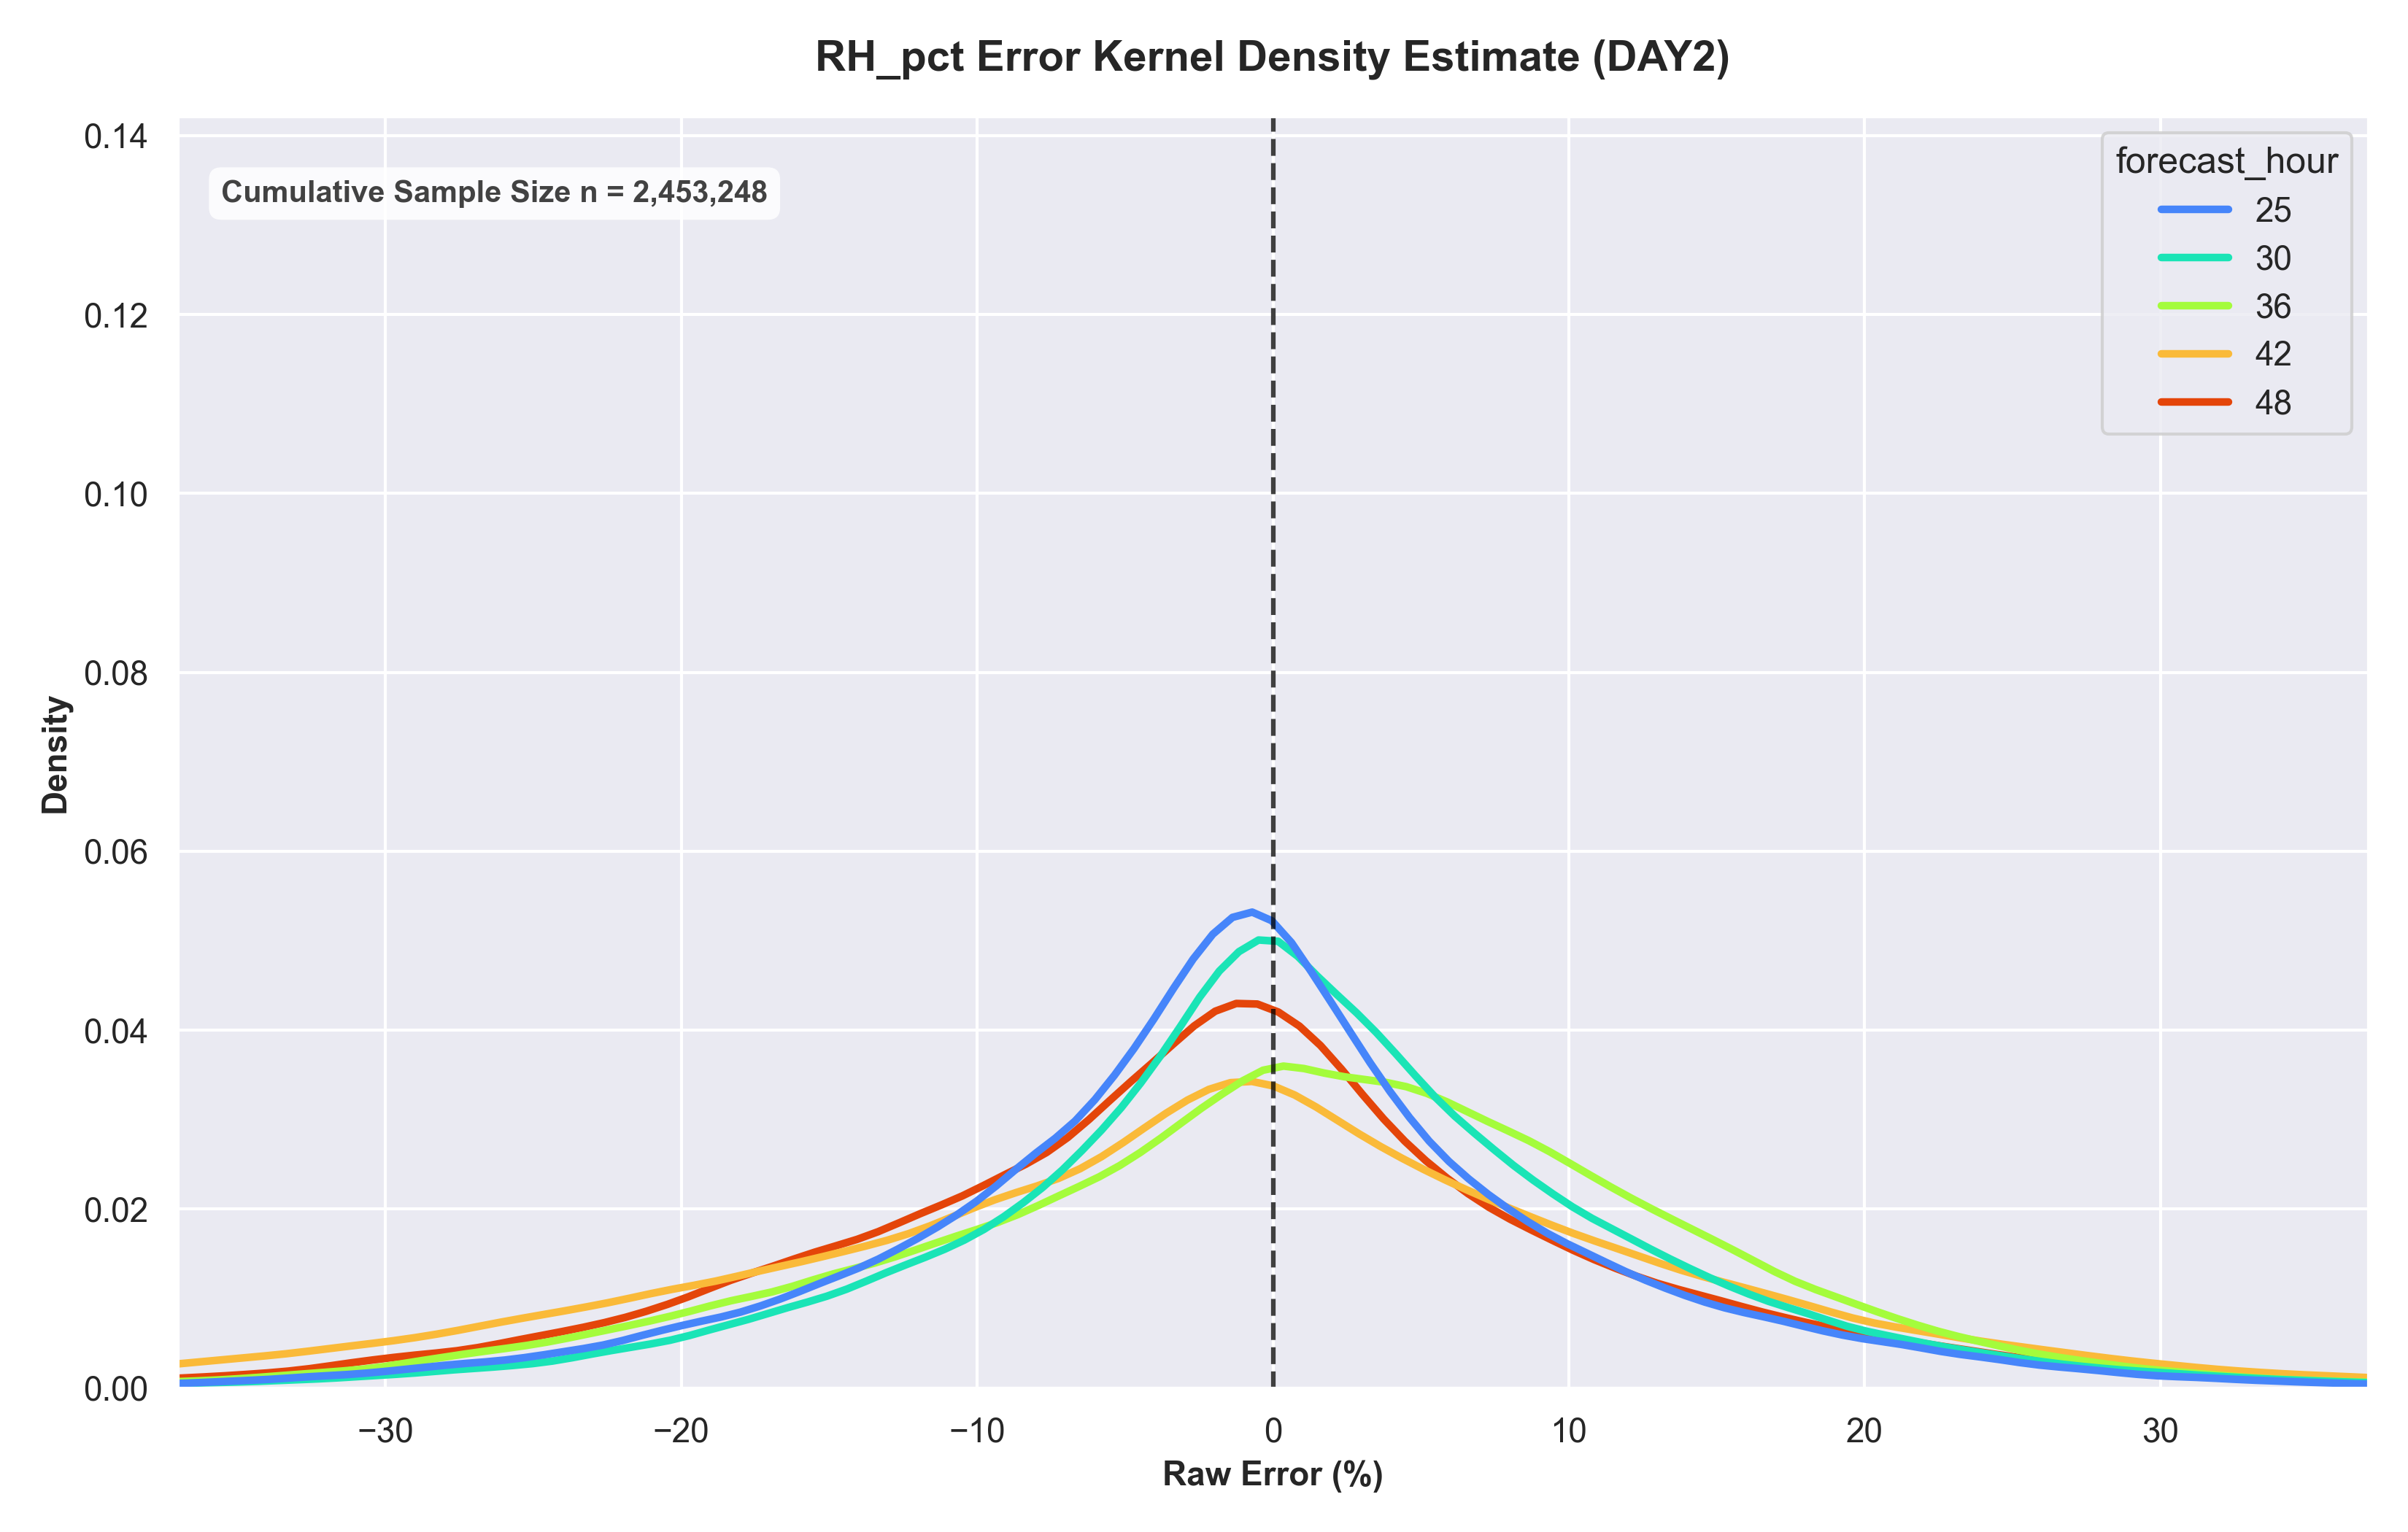
\includegraphics[width=0.49\textwidth]{figures/KDE_GRAPHS_RAW/rh_pct_kde_day2.png}
  \caption{Kernel Density Estimation (KDE) of Relative Humidity (RH) forecast errors for Day 1 (left) and Day 2 (right).}
  \label{fig:kde_rh}
\end{figure}

\begin{figure}[H]
  \centering
  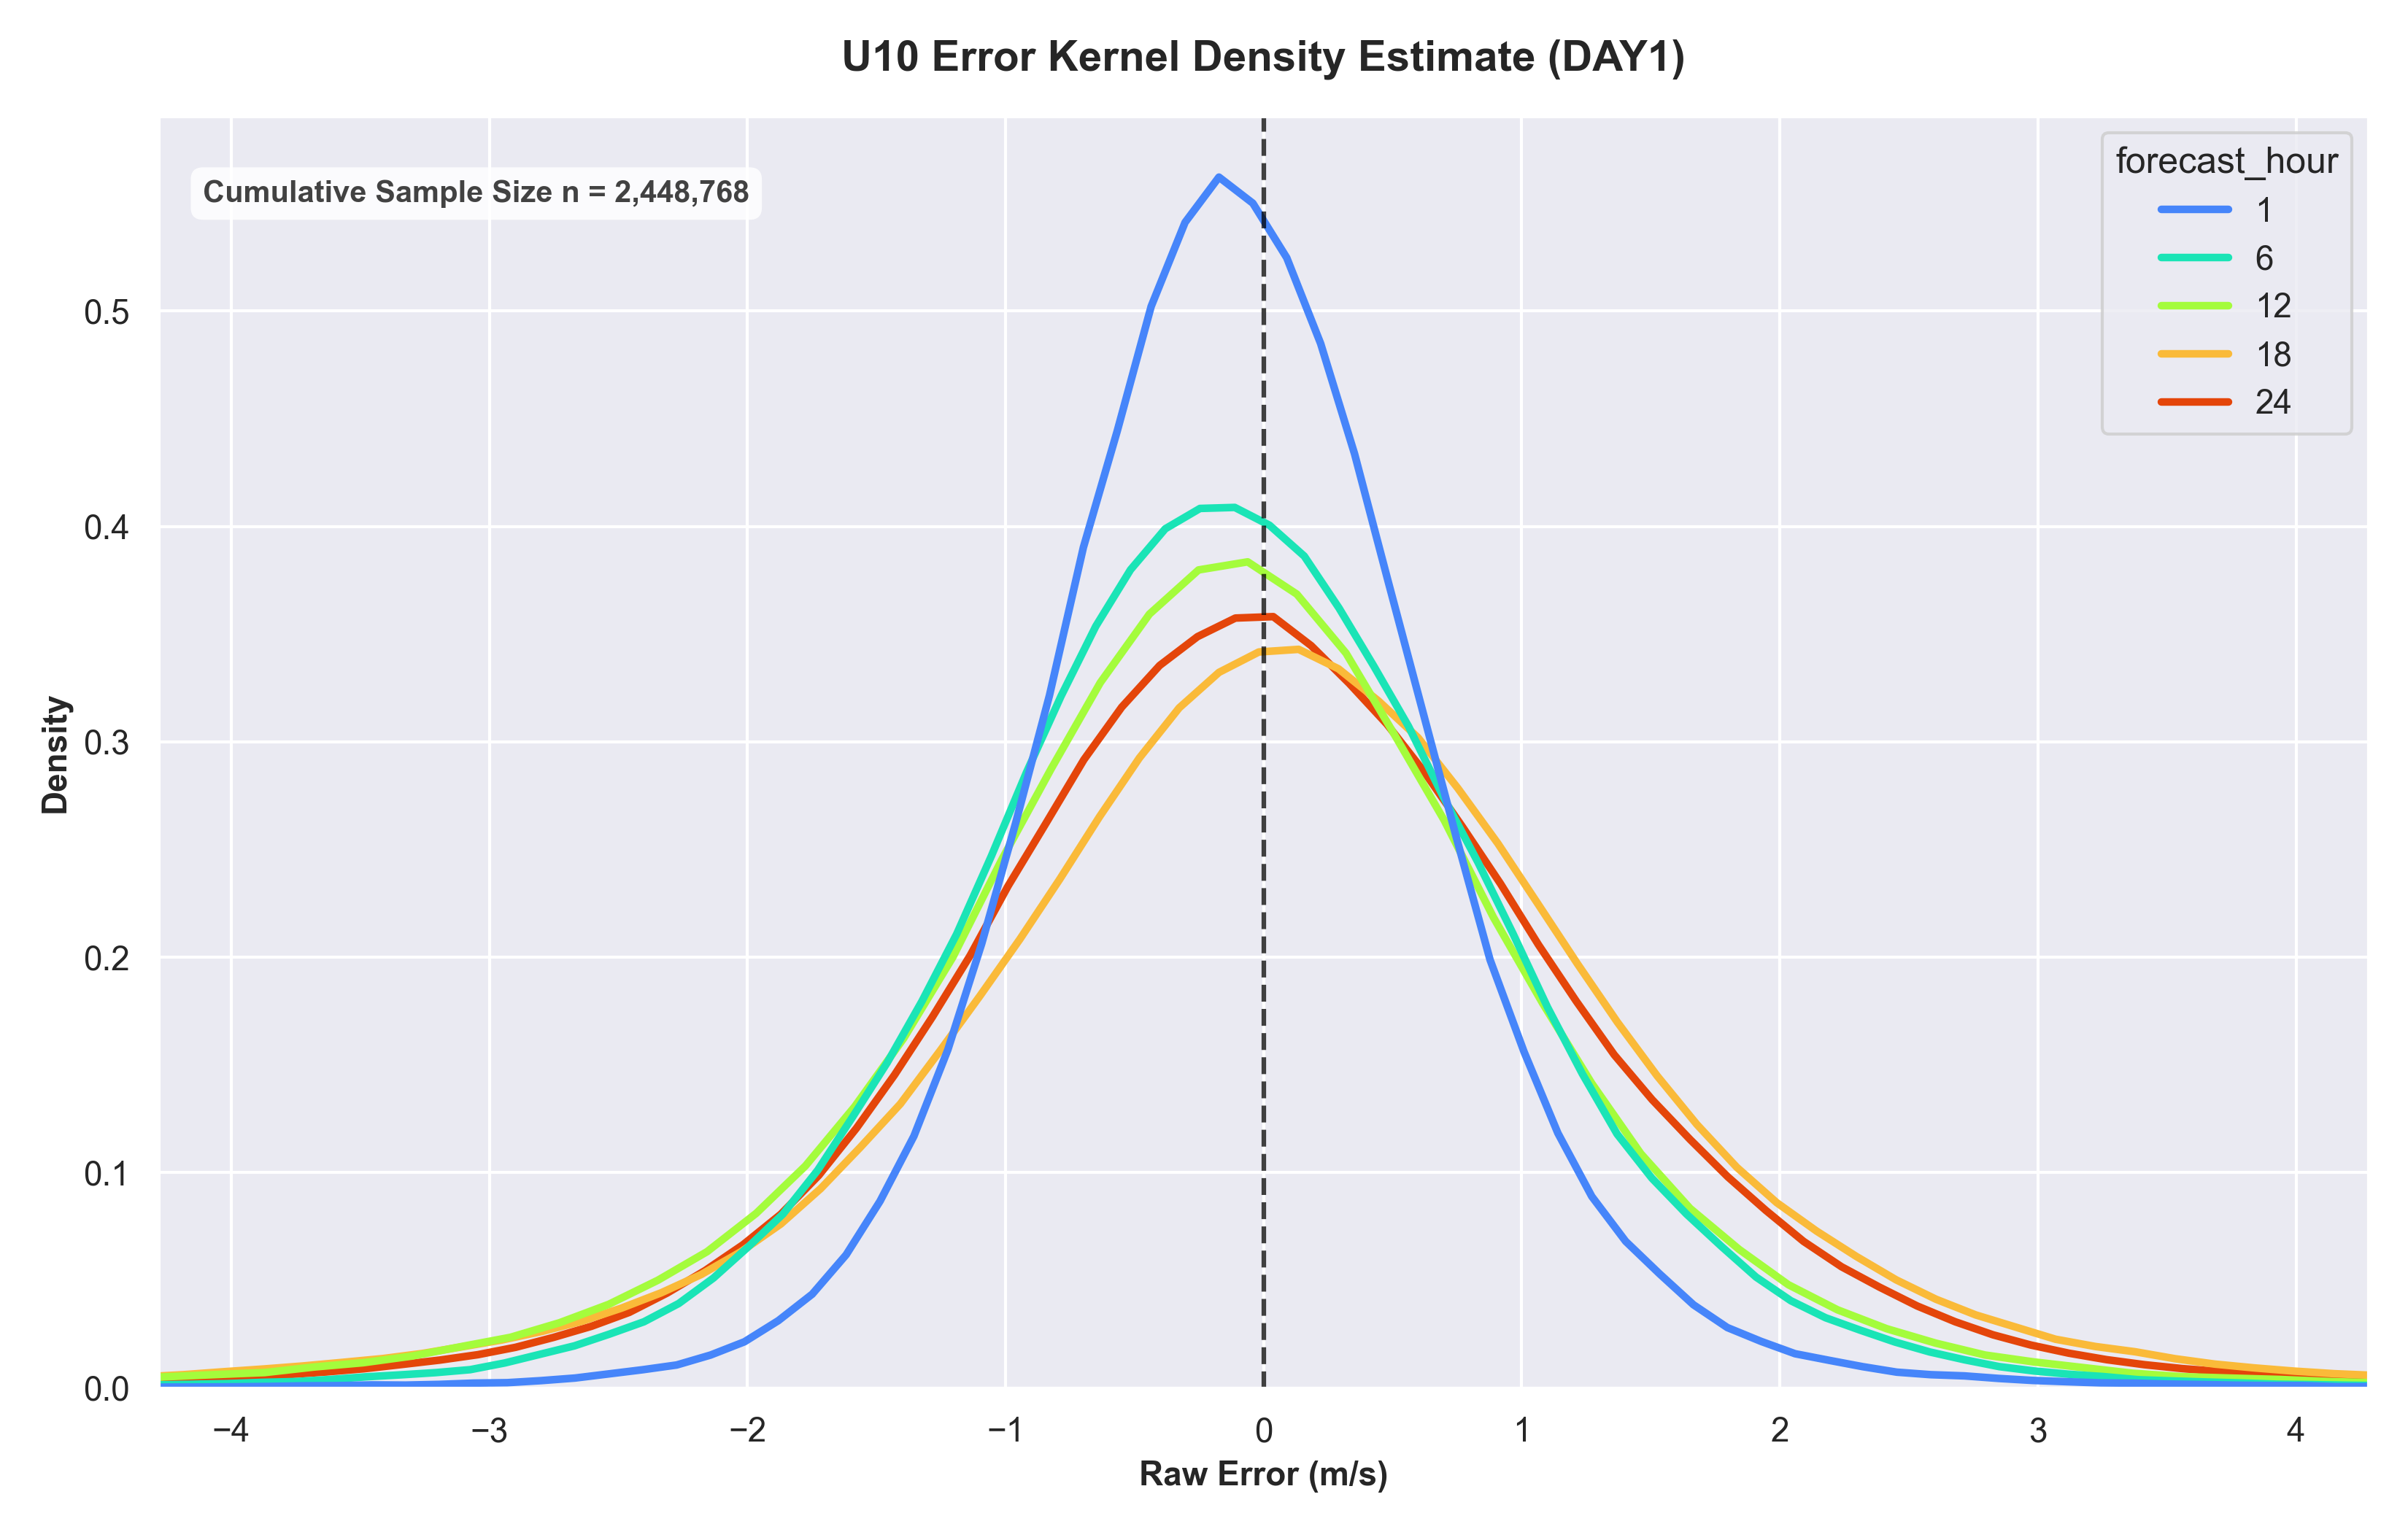
\includegraphics[width=0.49\textwidth]{figures/KDE_GRAPHS_RAW/u10_kde_day1.png}\hfill
  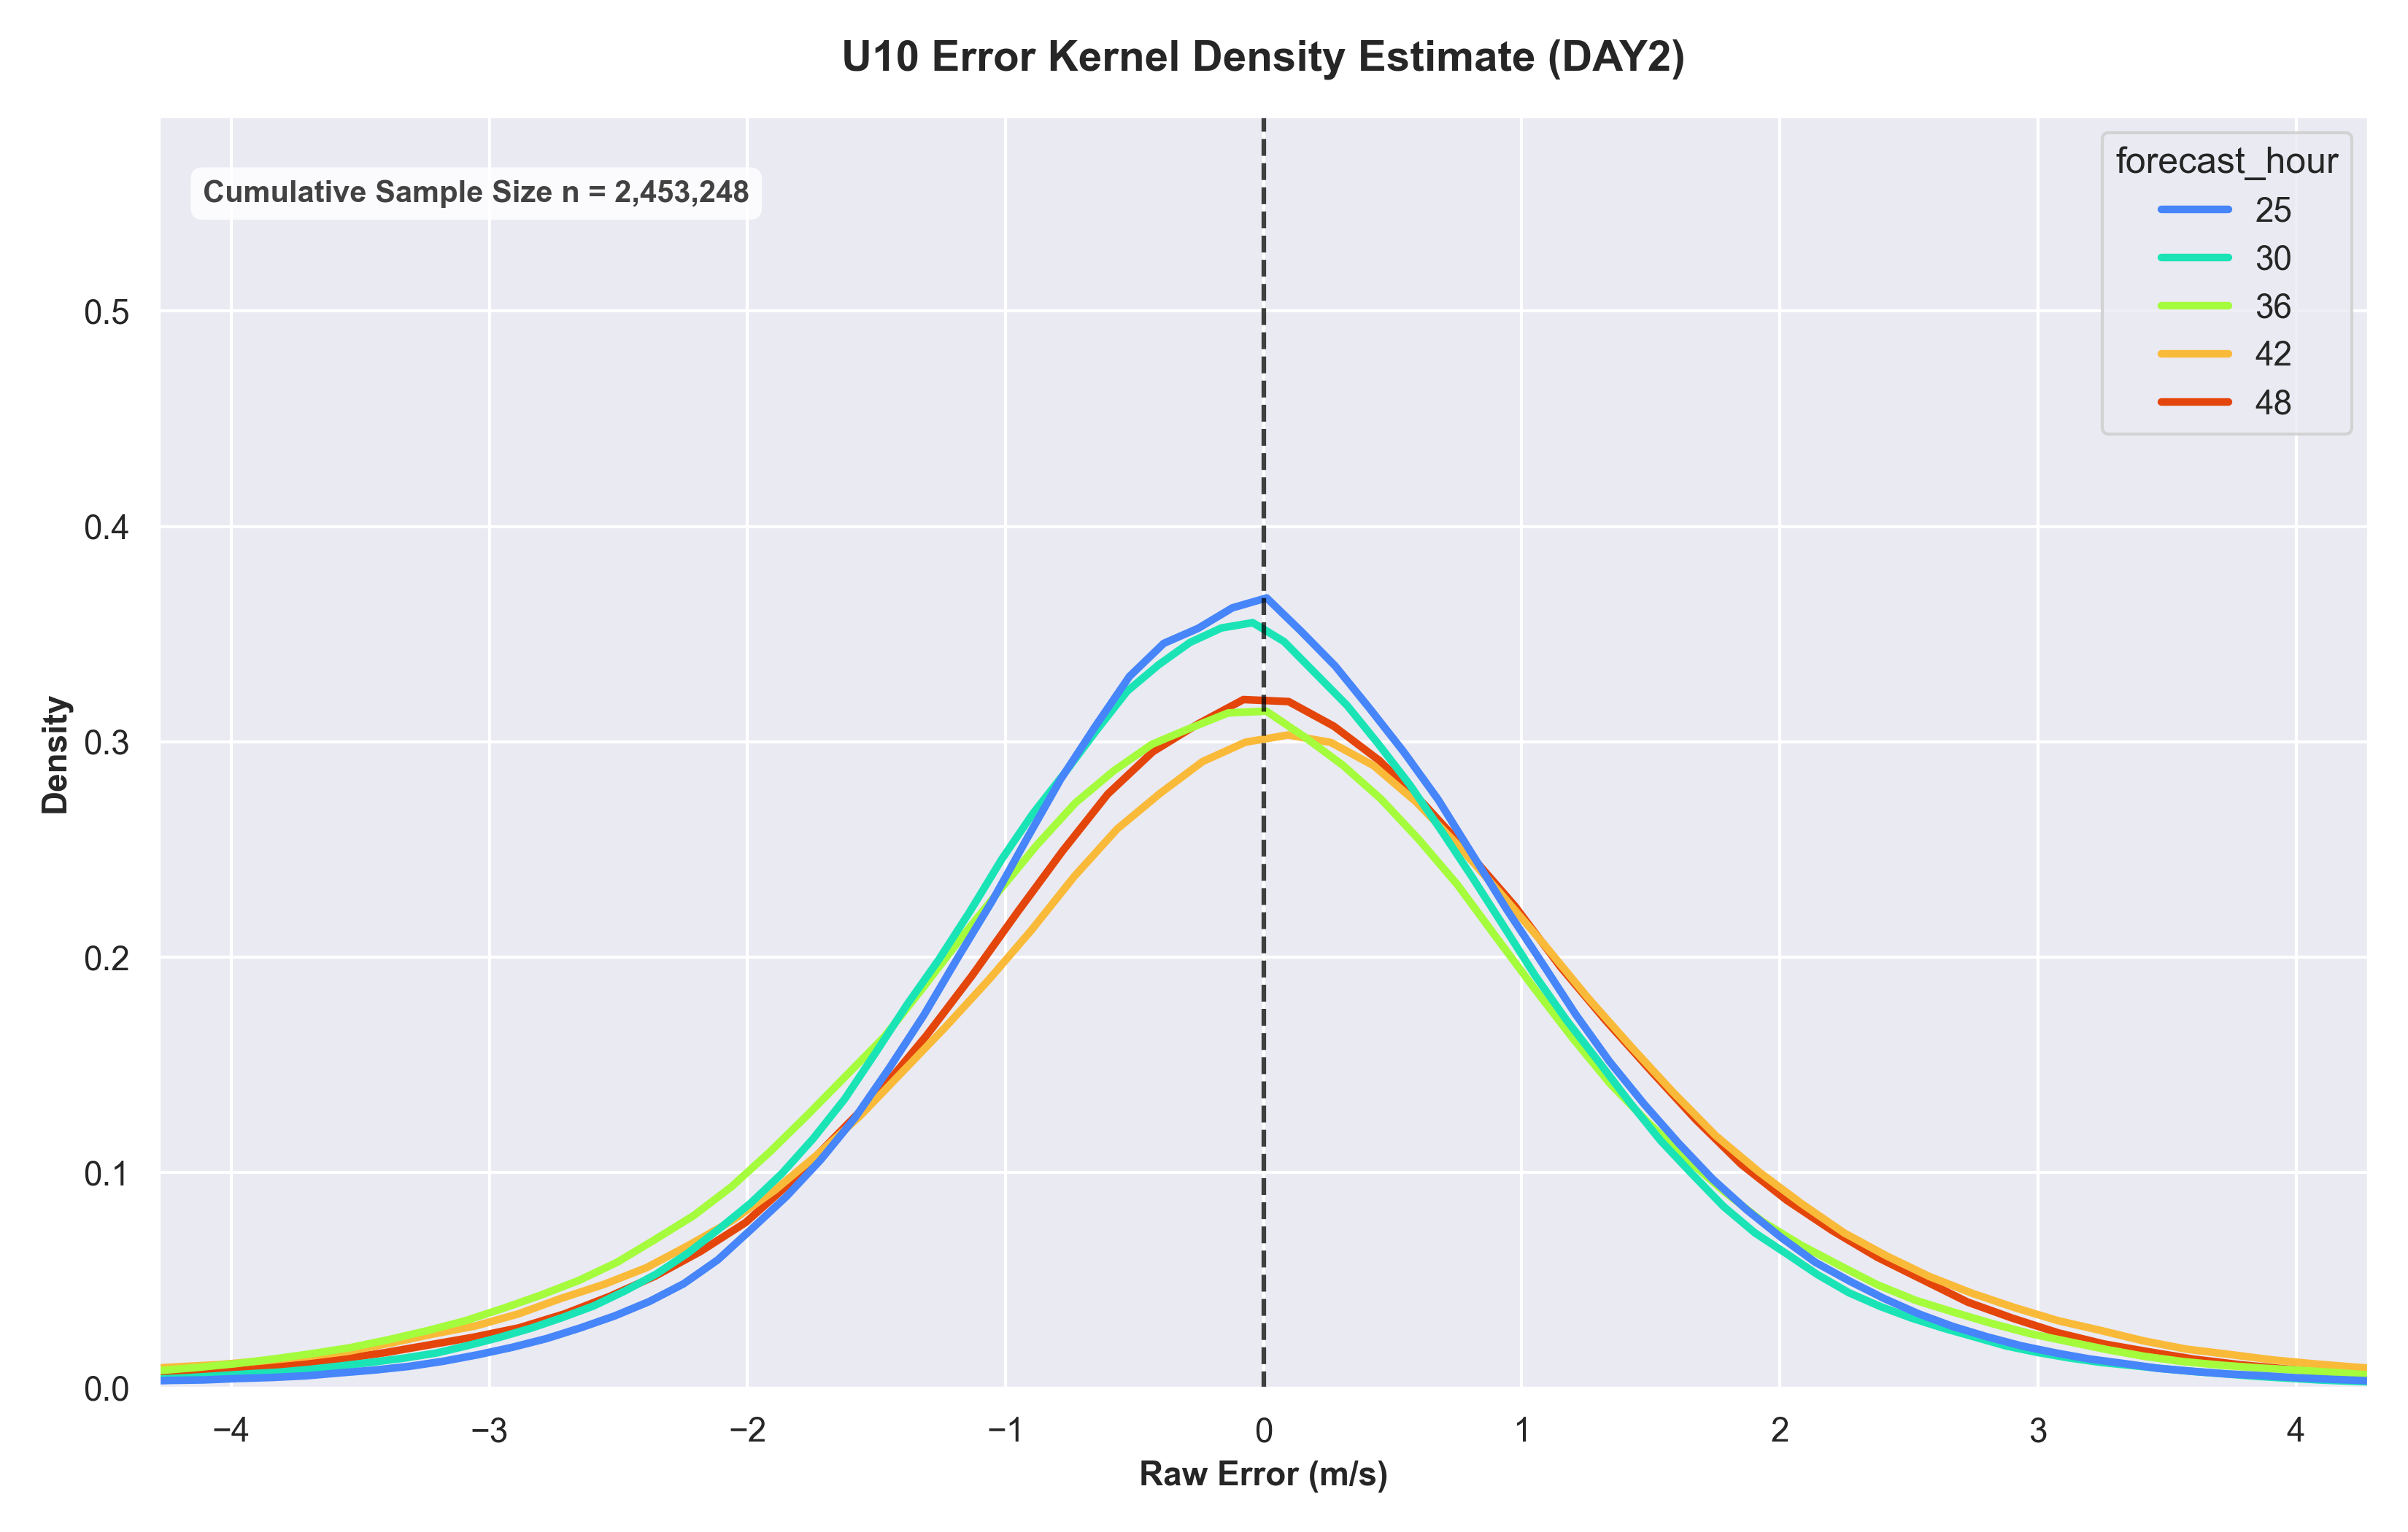
\includegraphics[width=0.49\textwidth]{figures/KDE_GRAPHS_RAW/u10_kde_day2.png}
  \caption{Kernel Density Estimation (KDE) of U10 wind component forecast errors for Day 1 (left) and Day 2 (right).}
  \label{fig:kde_u10}
\end{figure}

\begin{figure}[H]
  \centering
  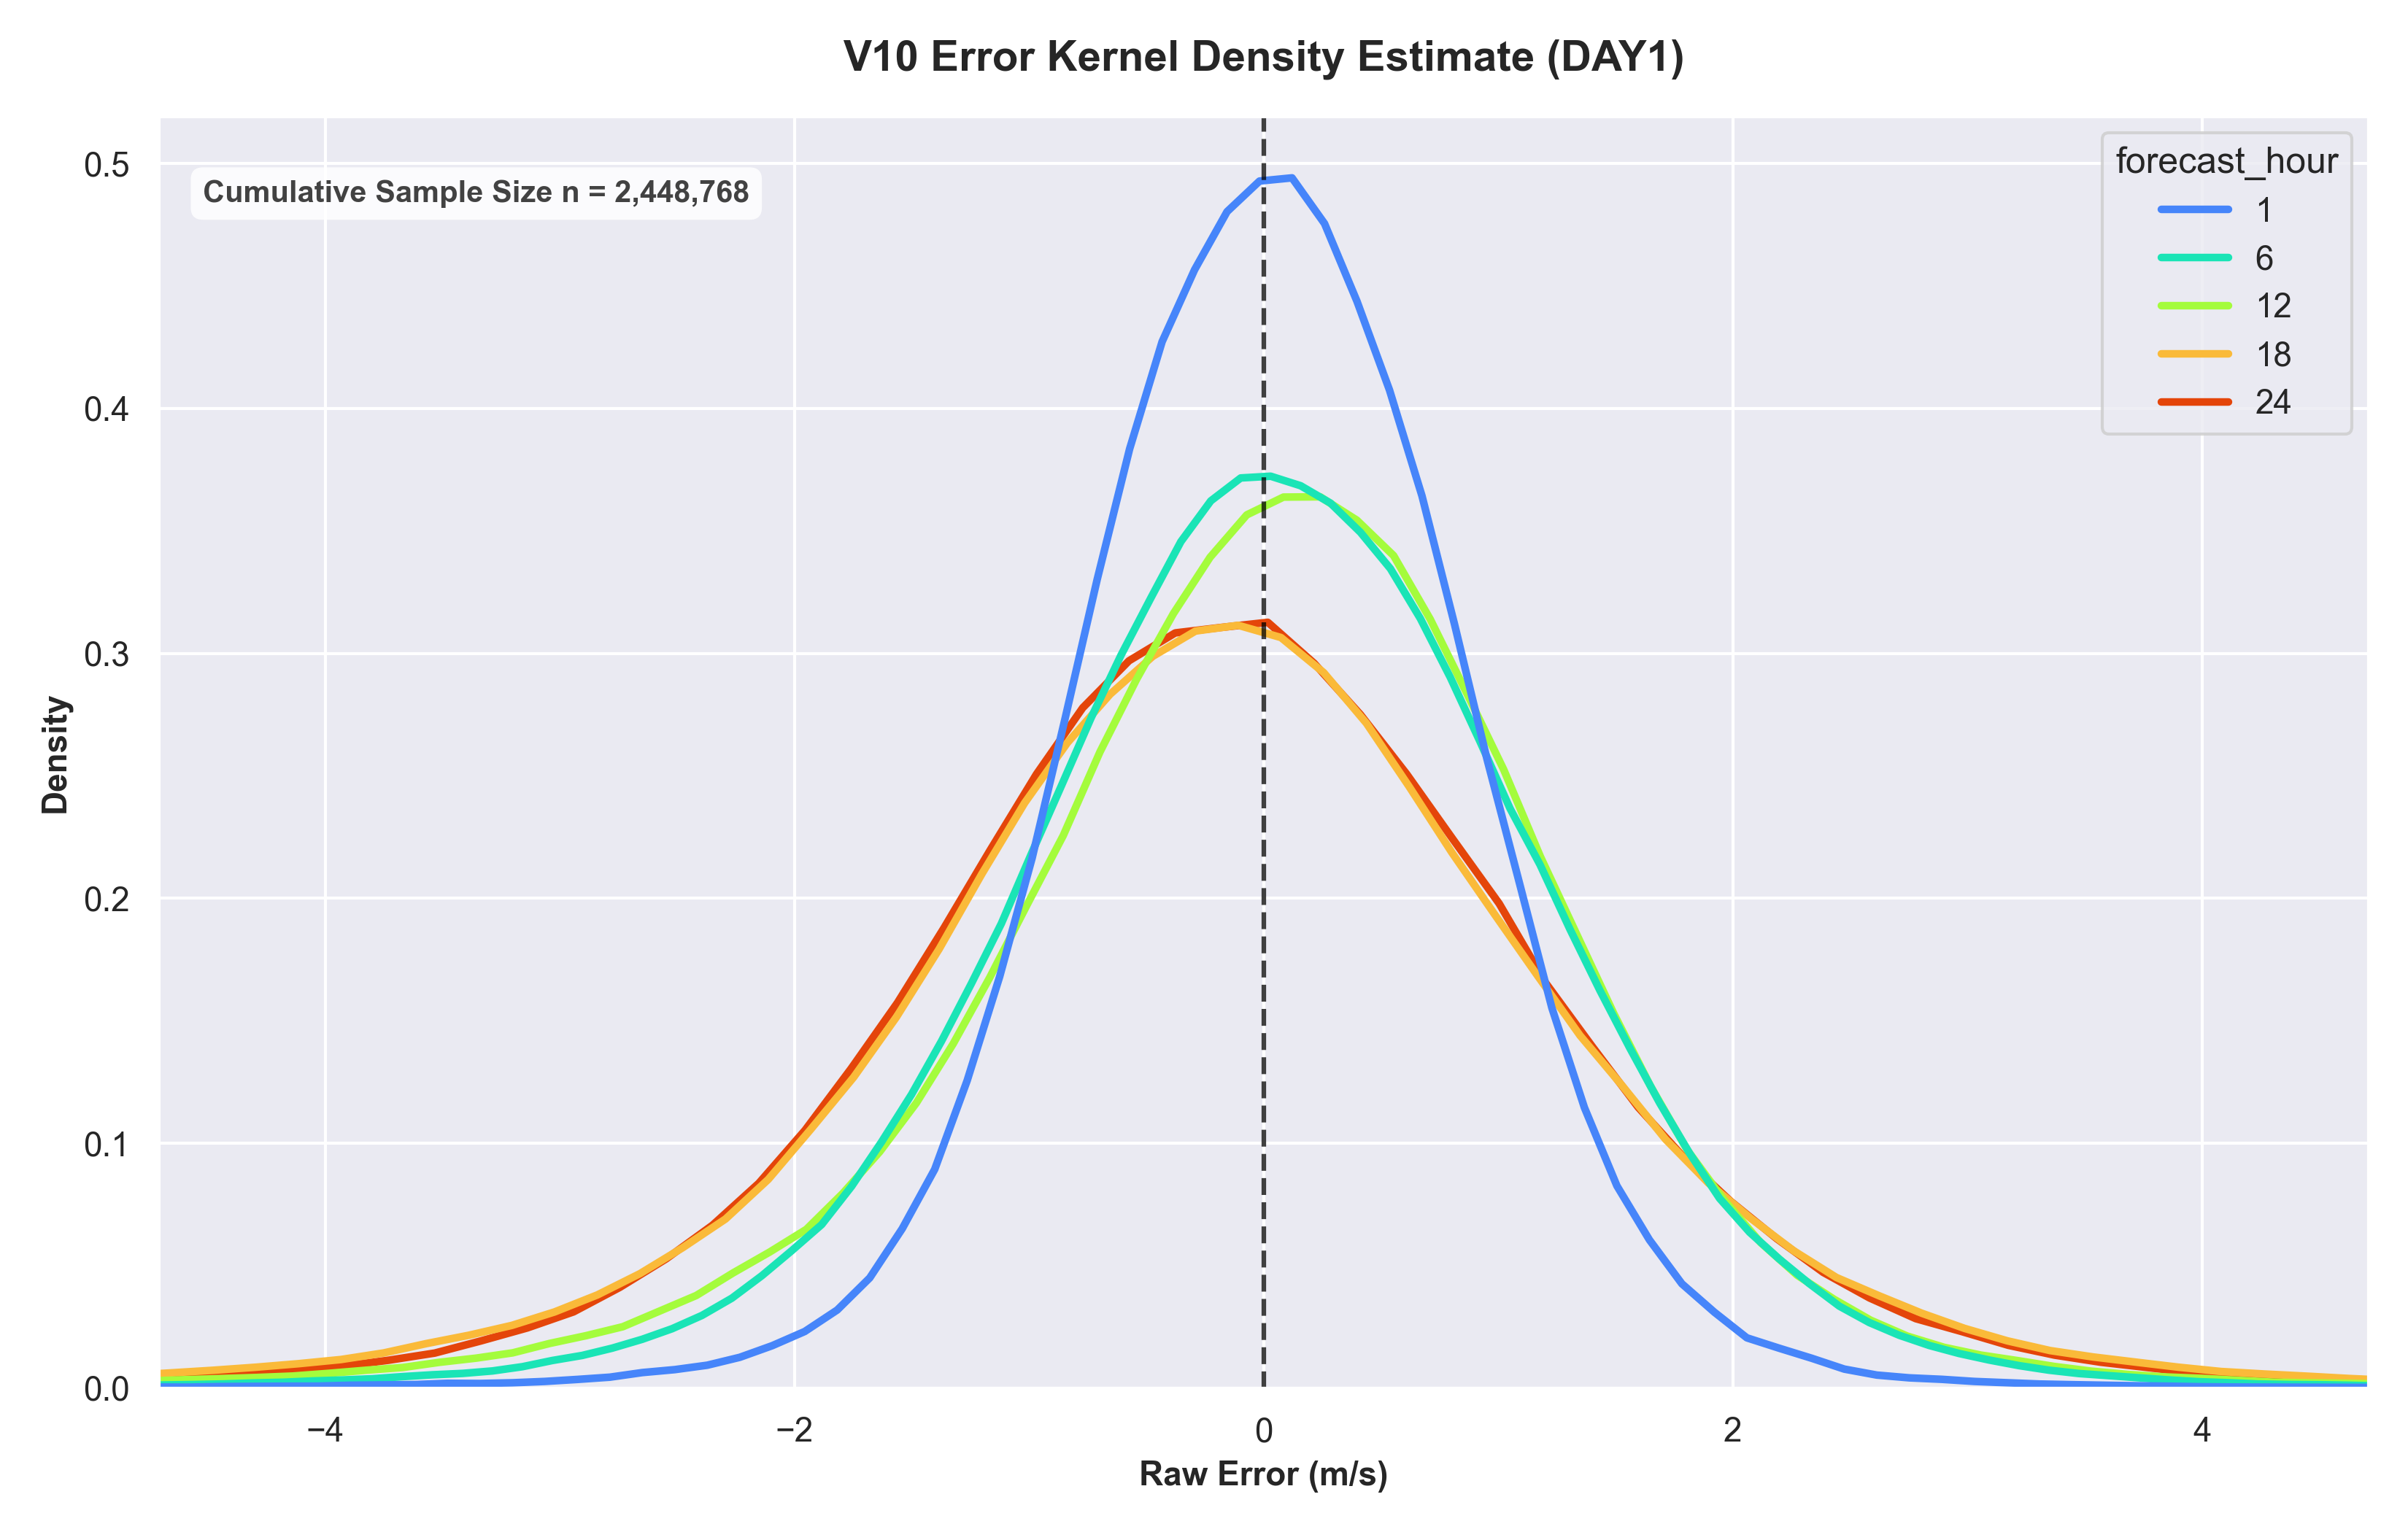
\includegraphics[width=0.49\textwidth]{figures/KDE_GRAPHS_RAW/v10_kde_day1.png}\hfill
  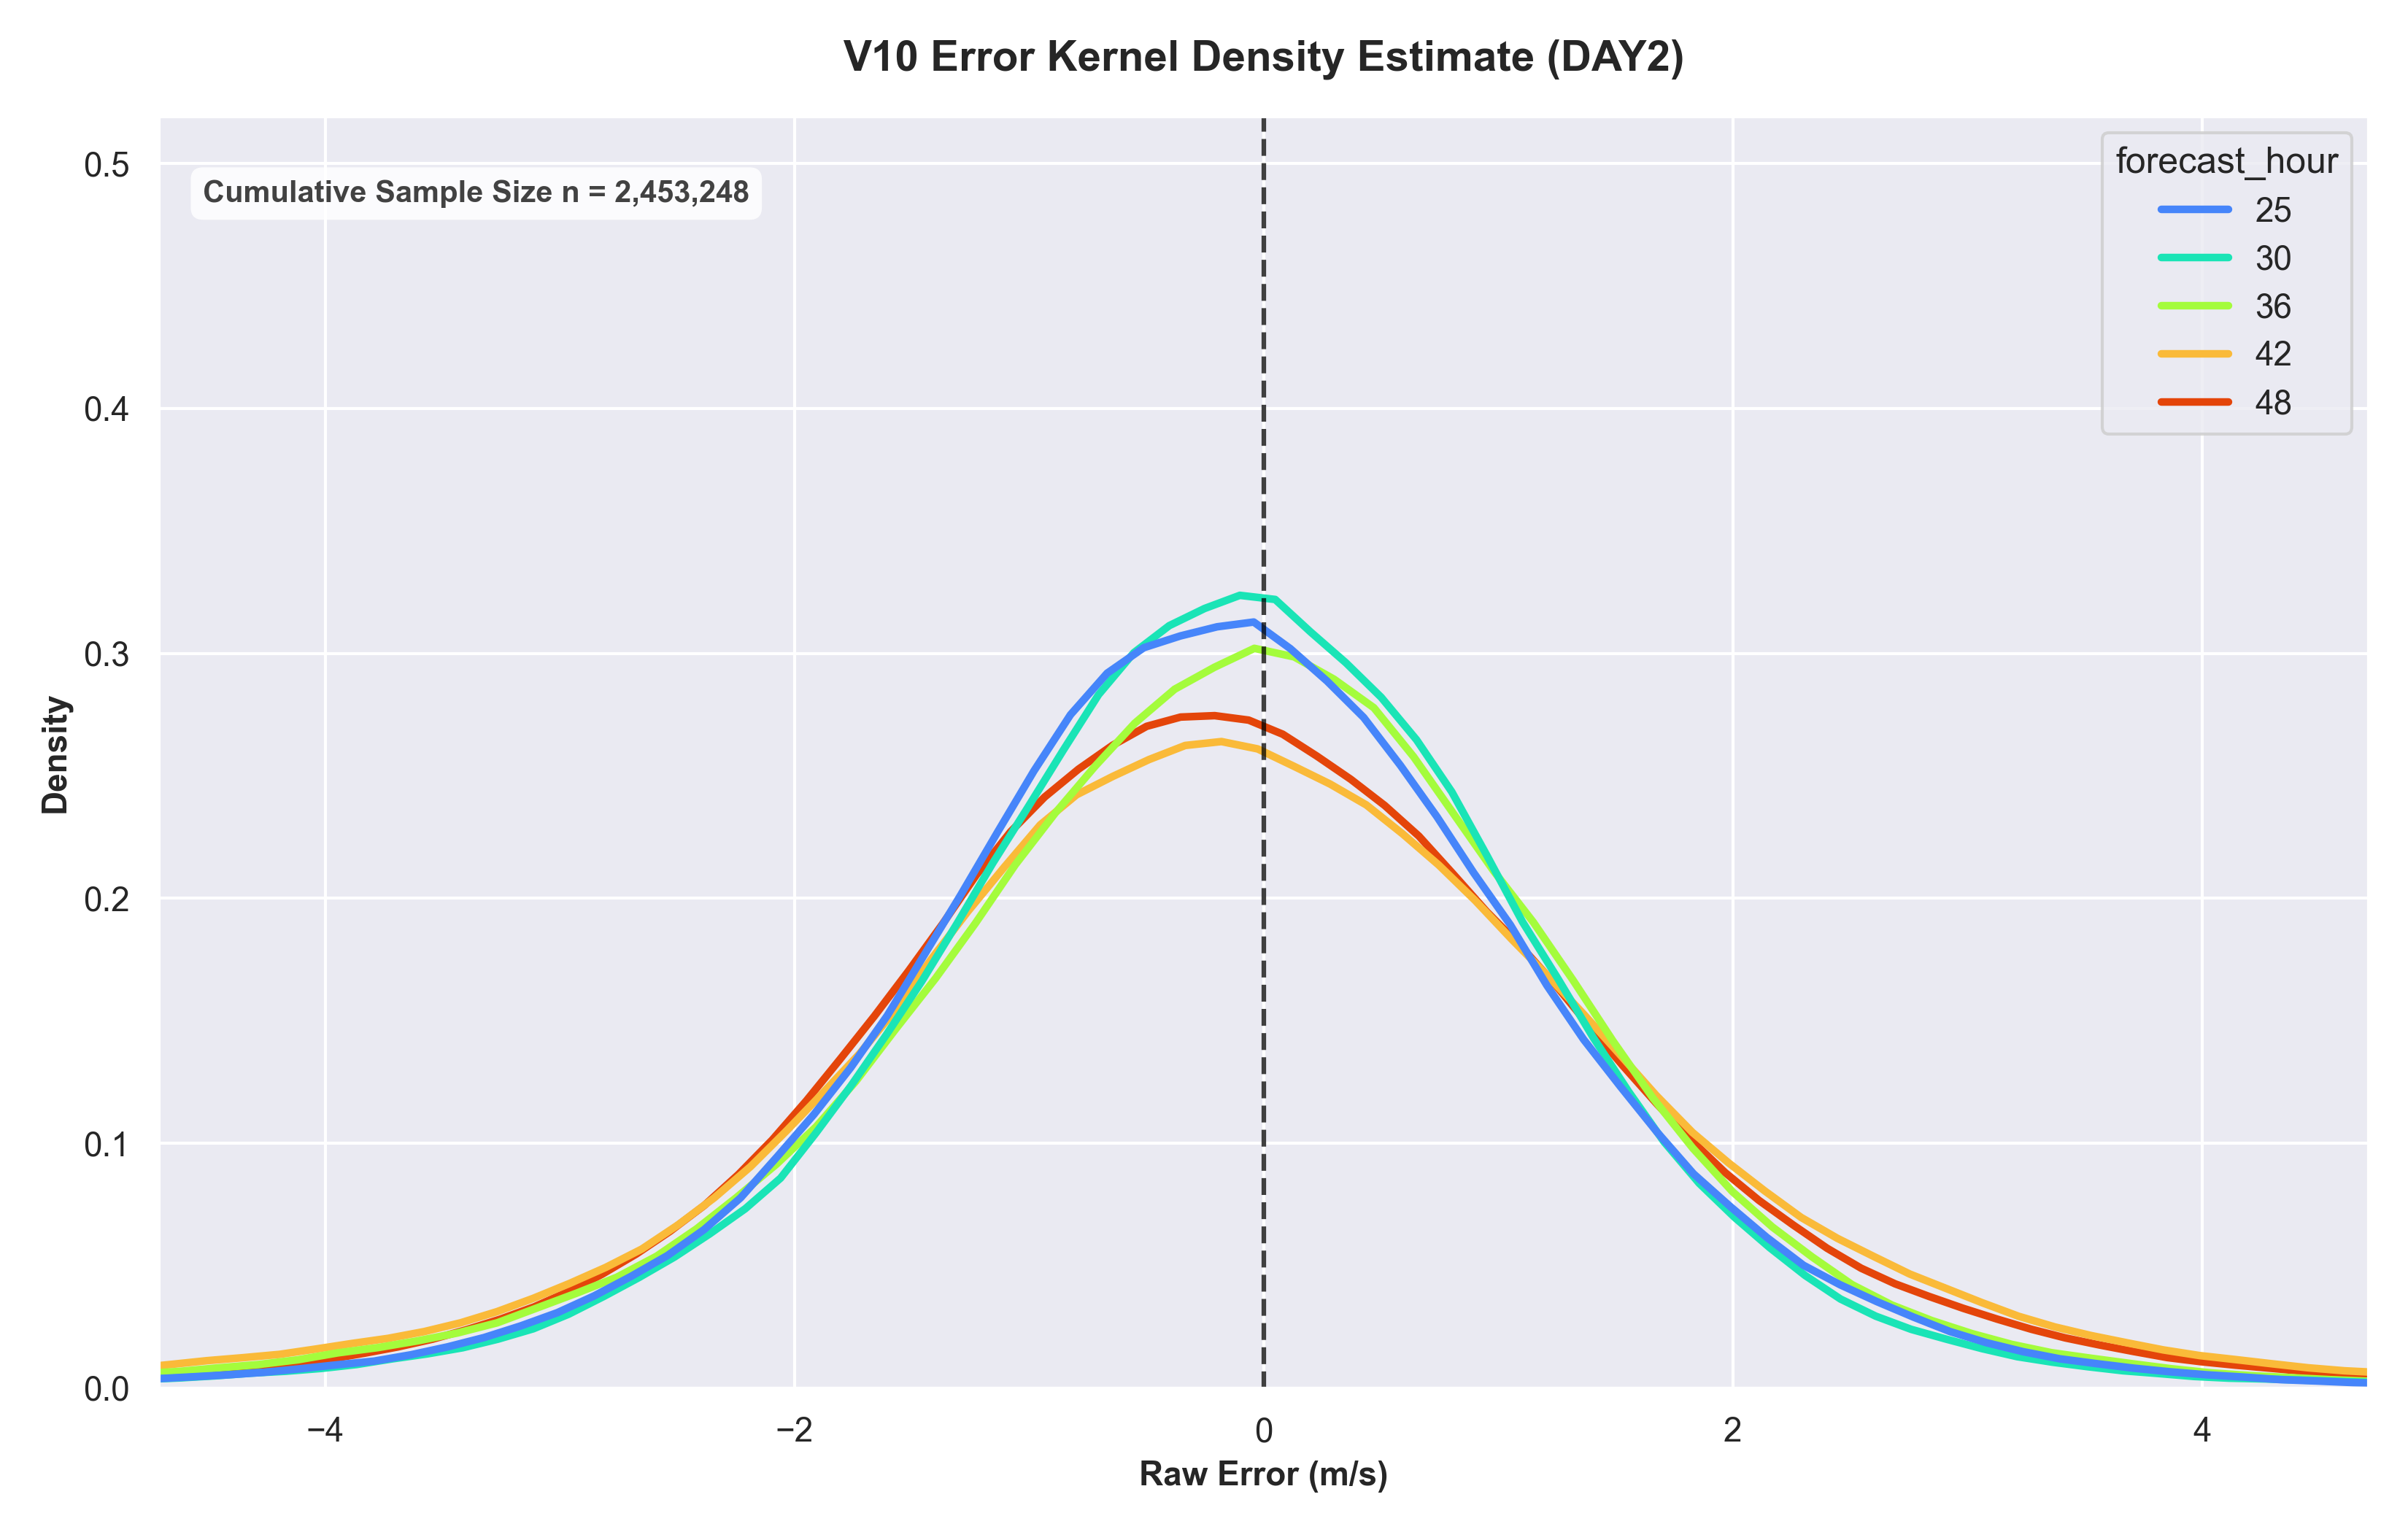
\includegraphics[width=0.49\textwidth]{figures/KDE_GRAPHS_RAW/v10_kde_day2.png}
  \caption{Kernel Density Estimation (KDE) of V10 wind component forecast errors for Day 1 (left) and Day 2 (right).}
  \label{fig:kde_v10}
\end{figure}

\begin{figure}[H]
  \centering
  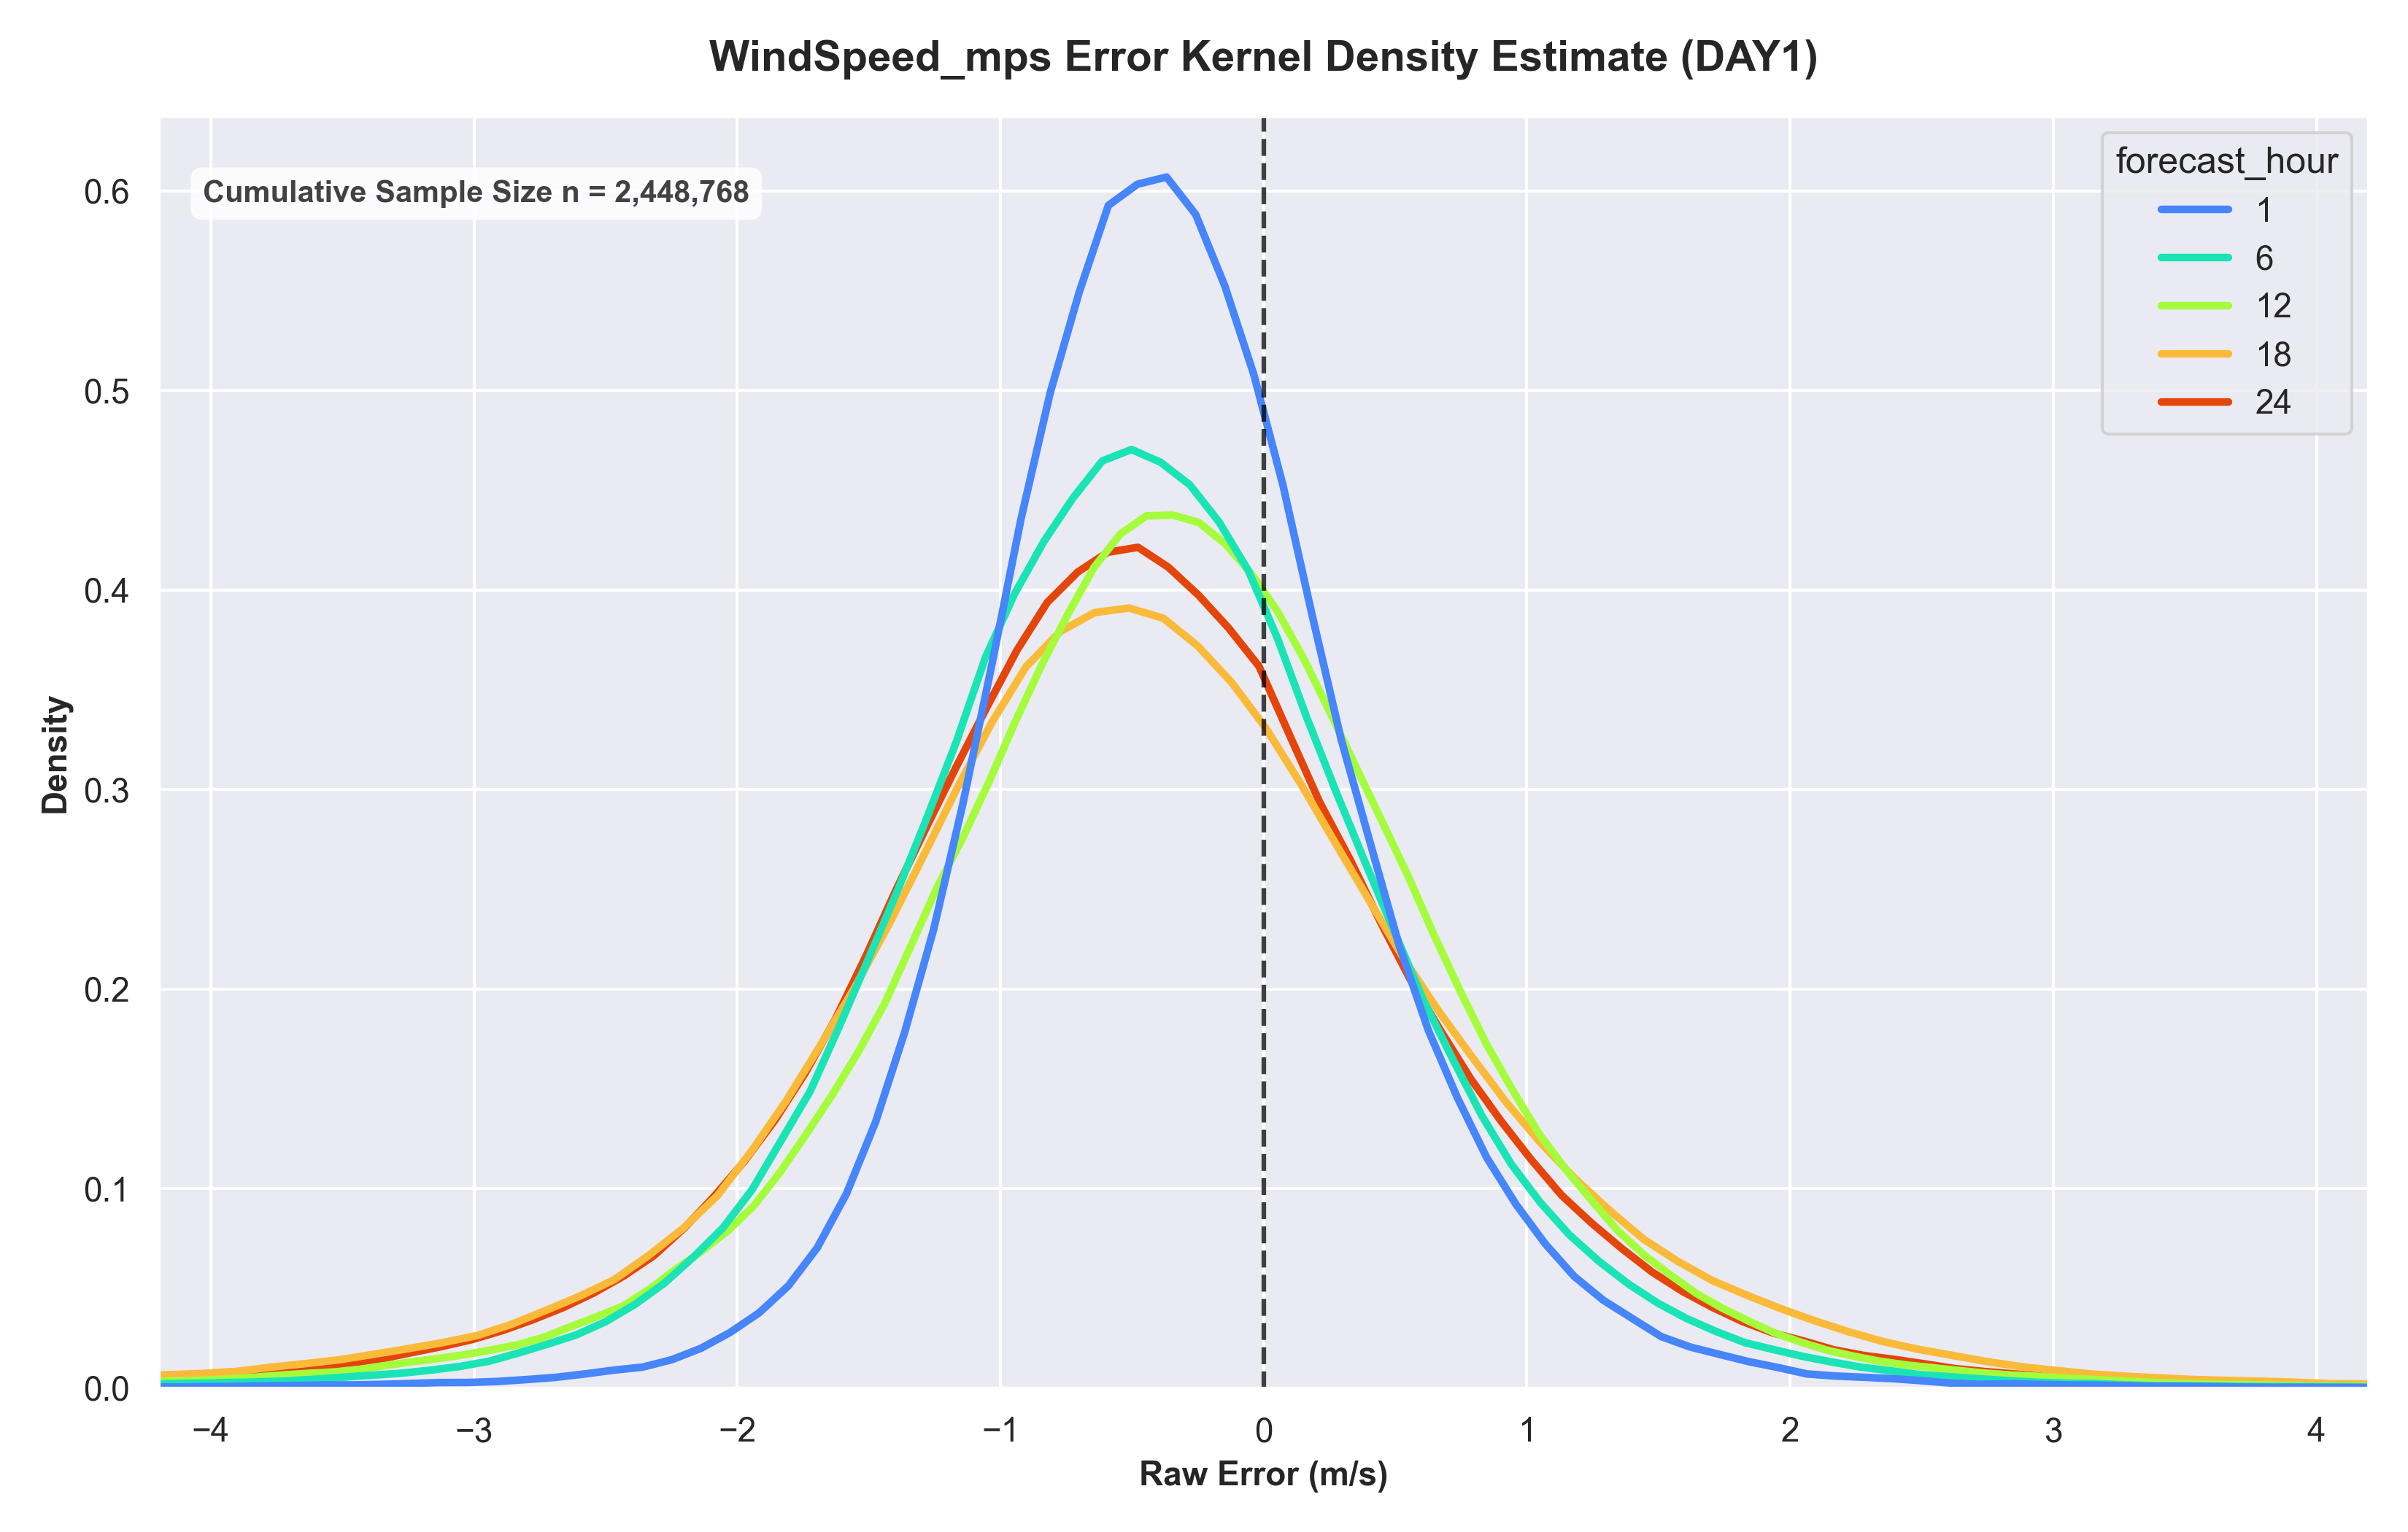
\includegraphics[width=0.49\textwidth]{figures/KDE_GRAPHS_RAW/windspeed_mps_kde_day1.png}\hfill
  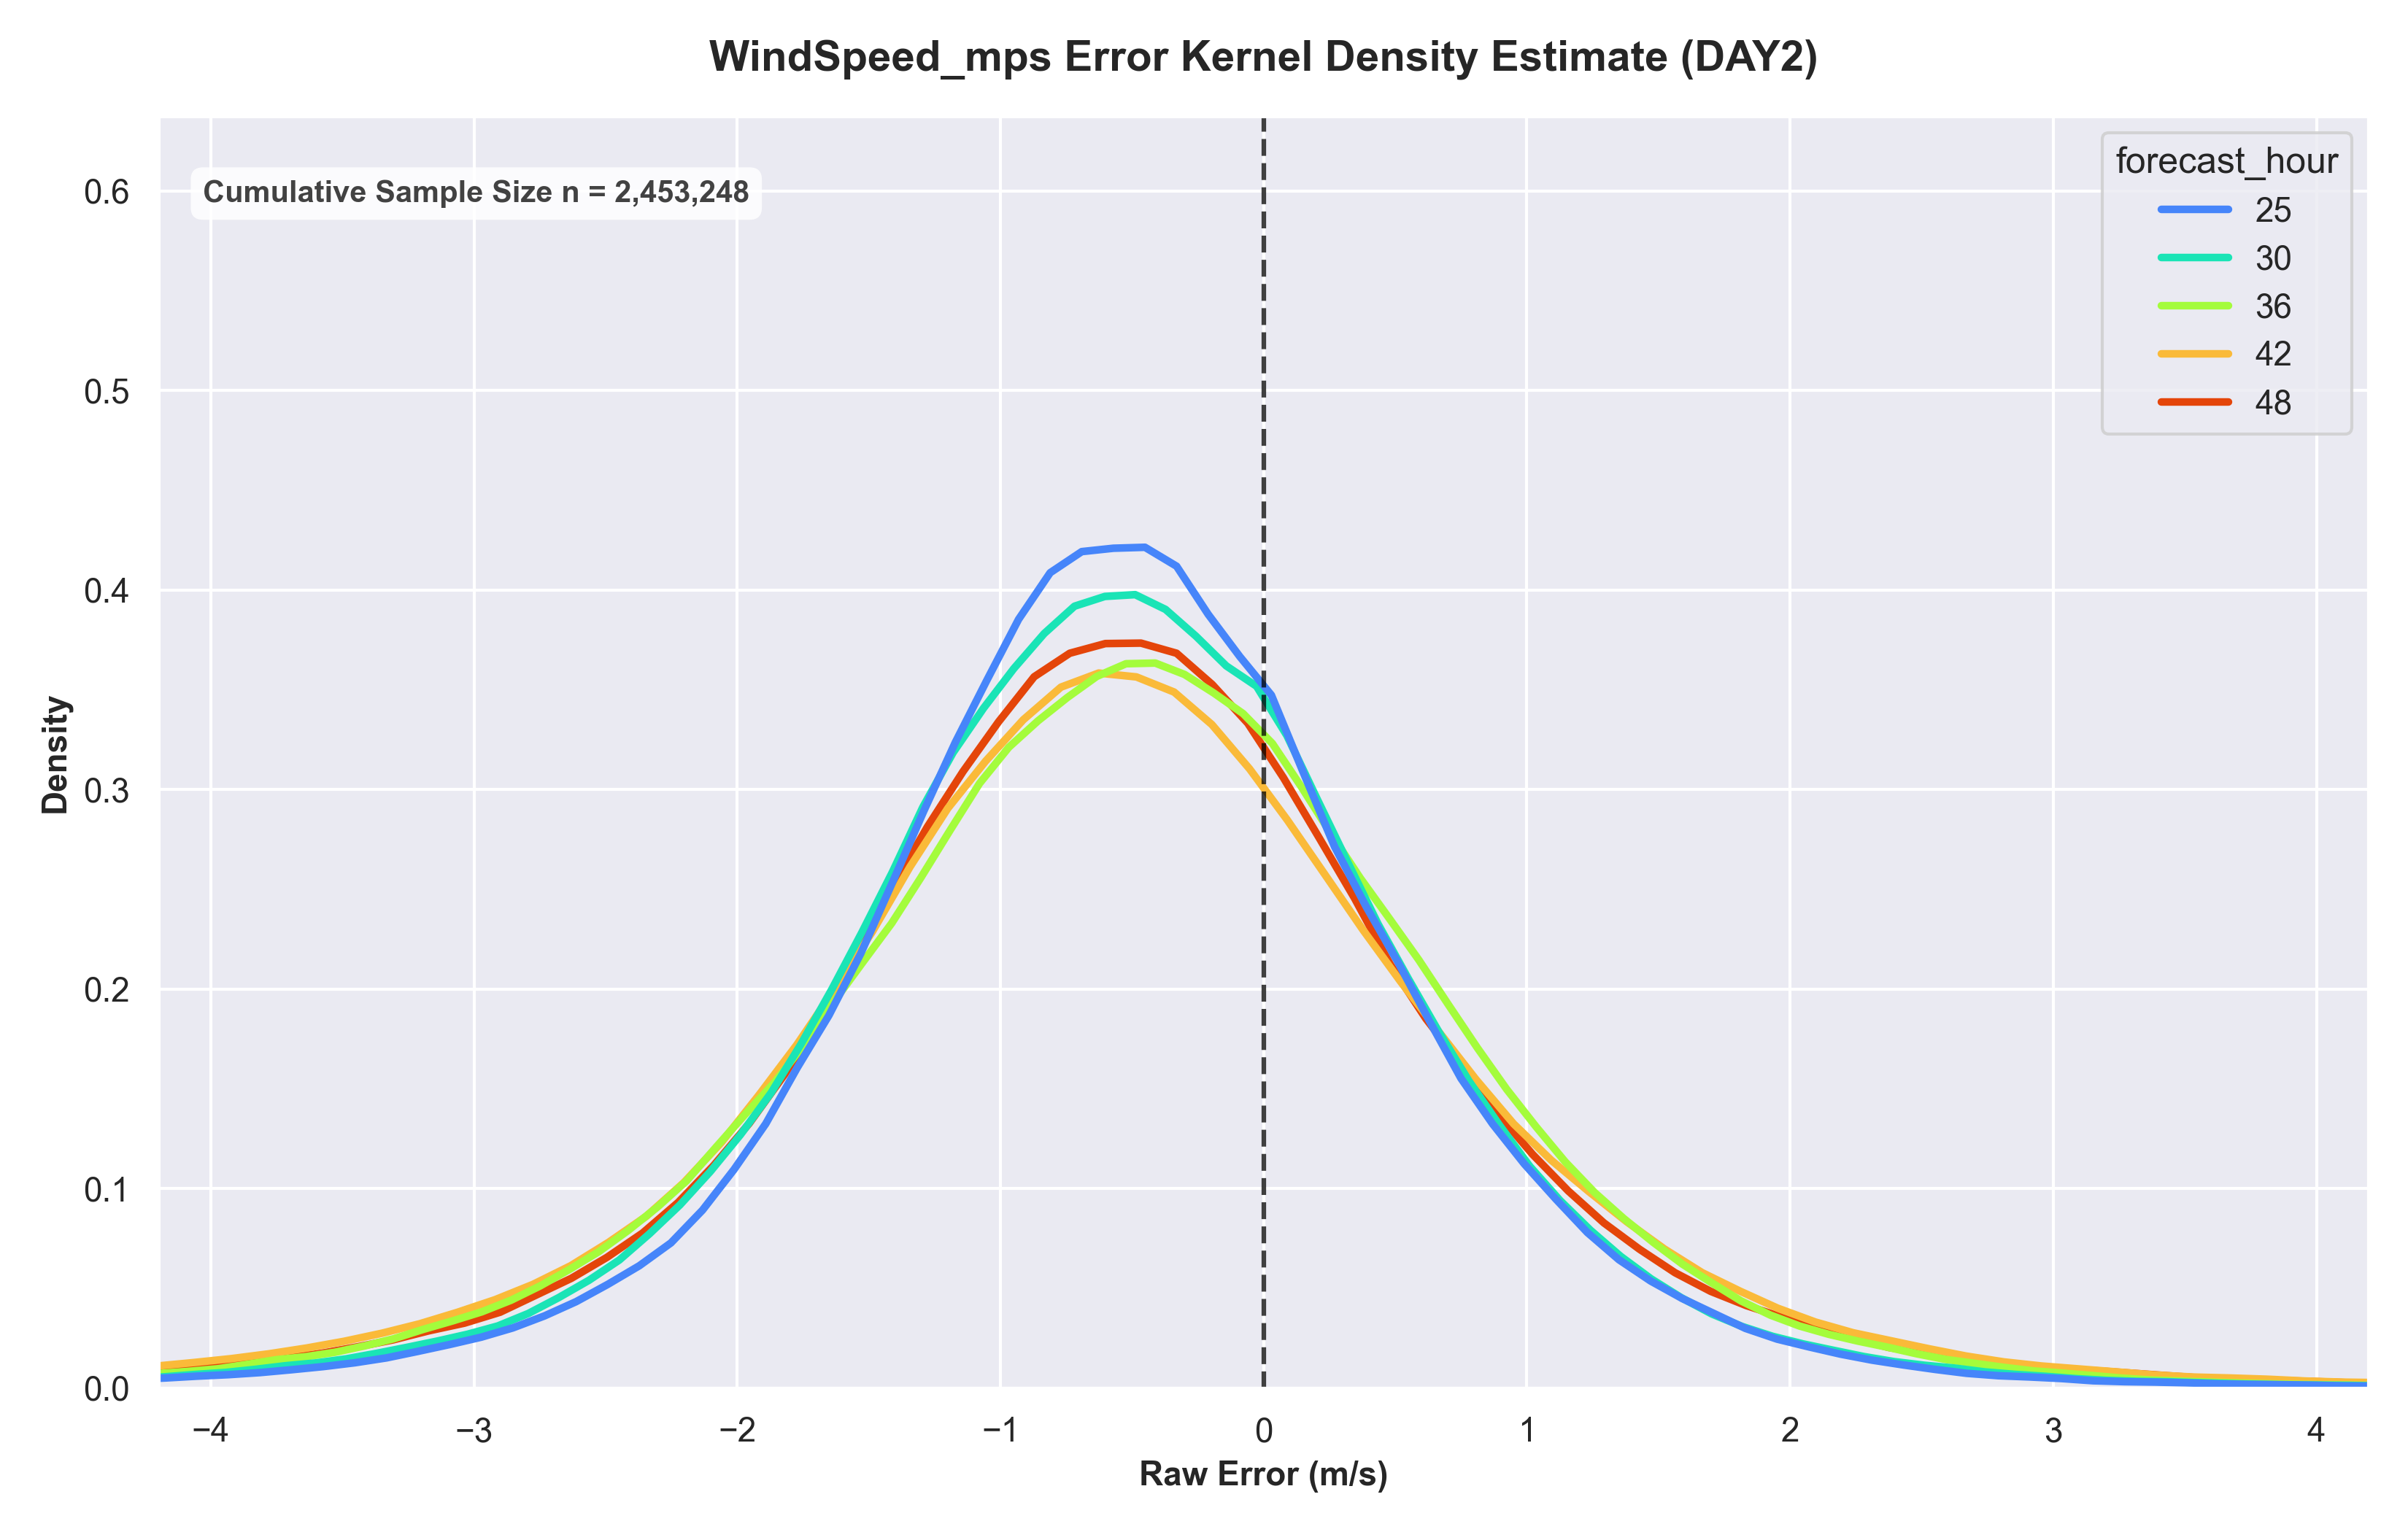
\includegraphics[width=0.49\textwidth]{figures/KDE_GRAPHS_RAW/windspeed_mps_kde_day2.png}
  \caption{Kernel Density Estimation (KDE) of Wind Speed forecast errors for Day 1 (left) and Day 2 (right).}
  \label{fig:kde_windspeed}
\end{figure}

\begin{figure}[H]
  \centering
  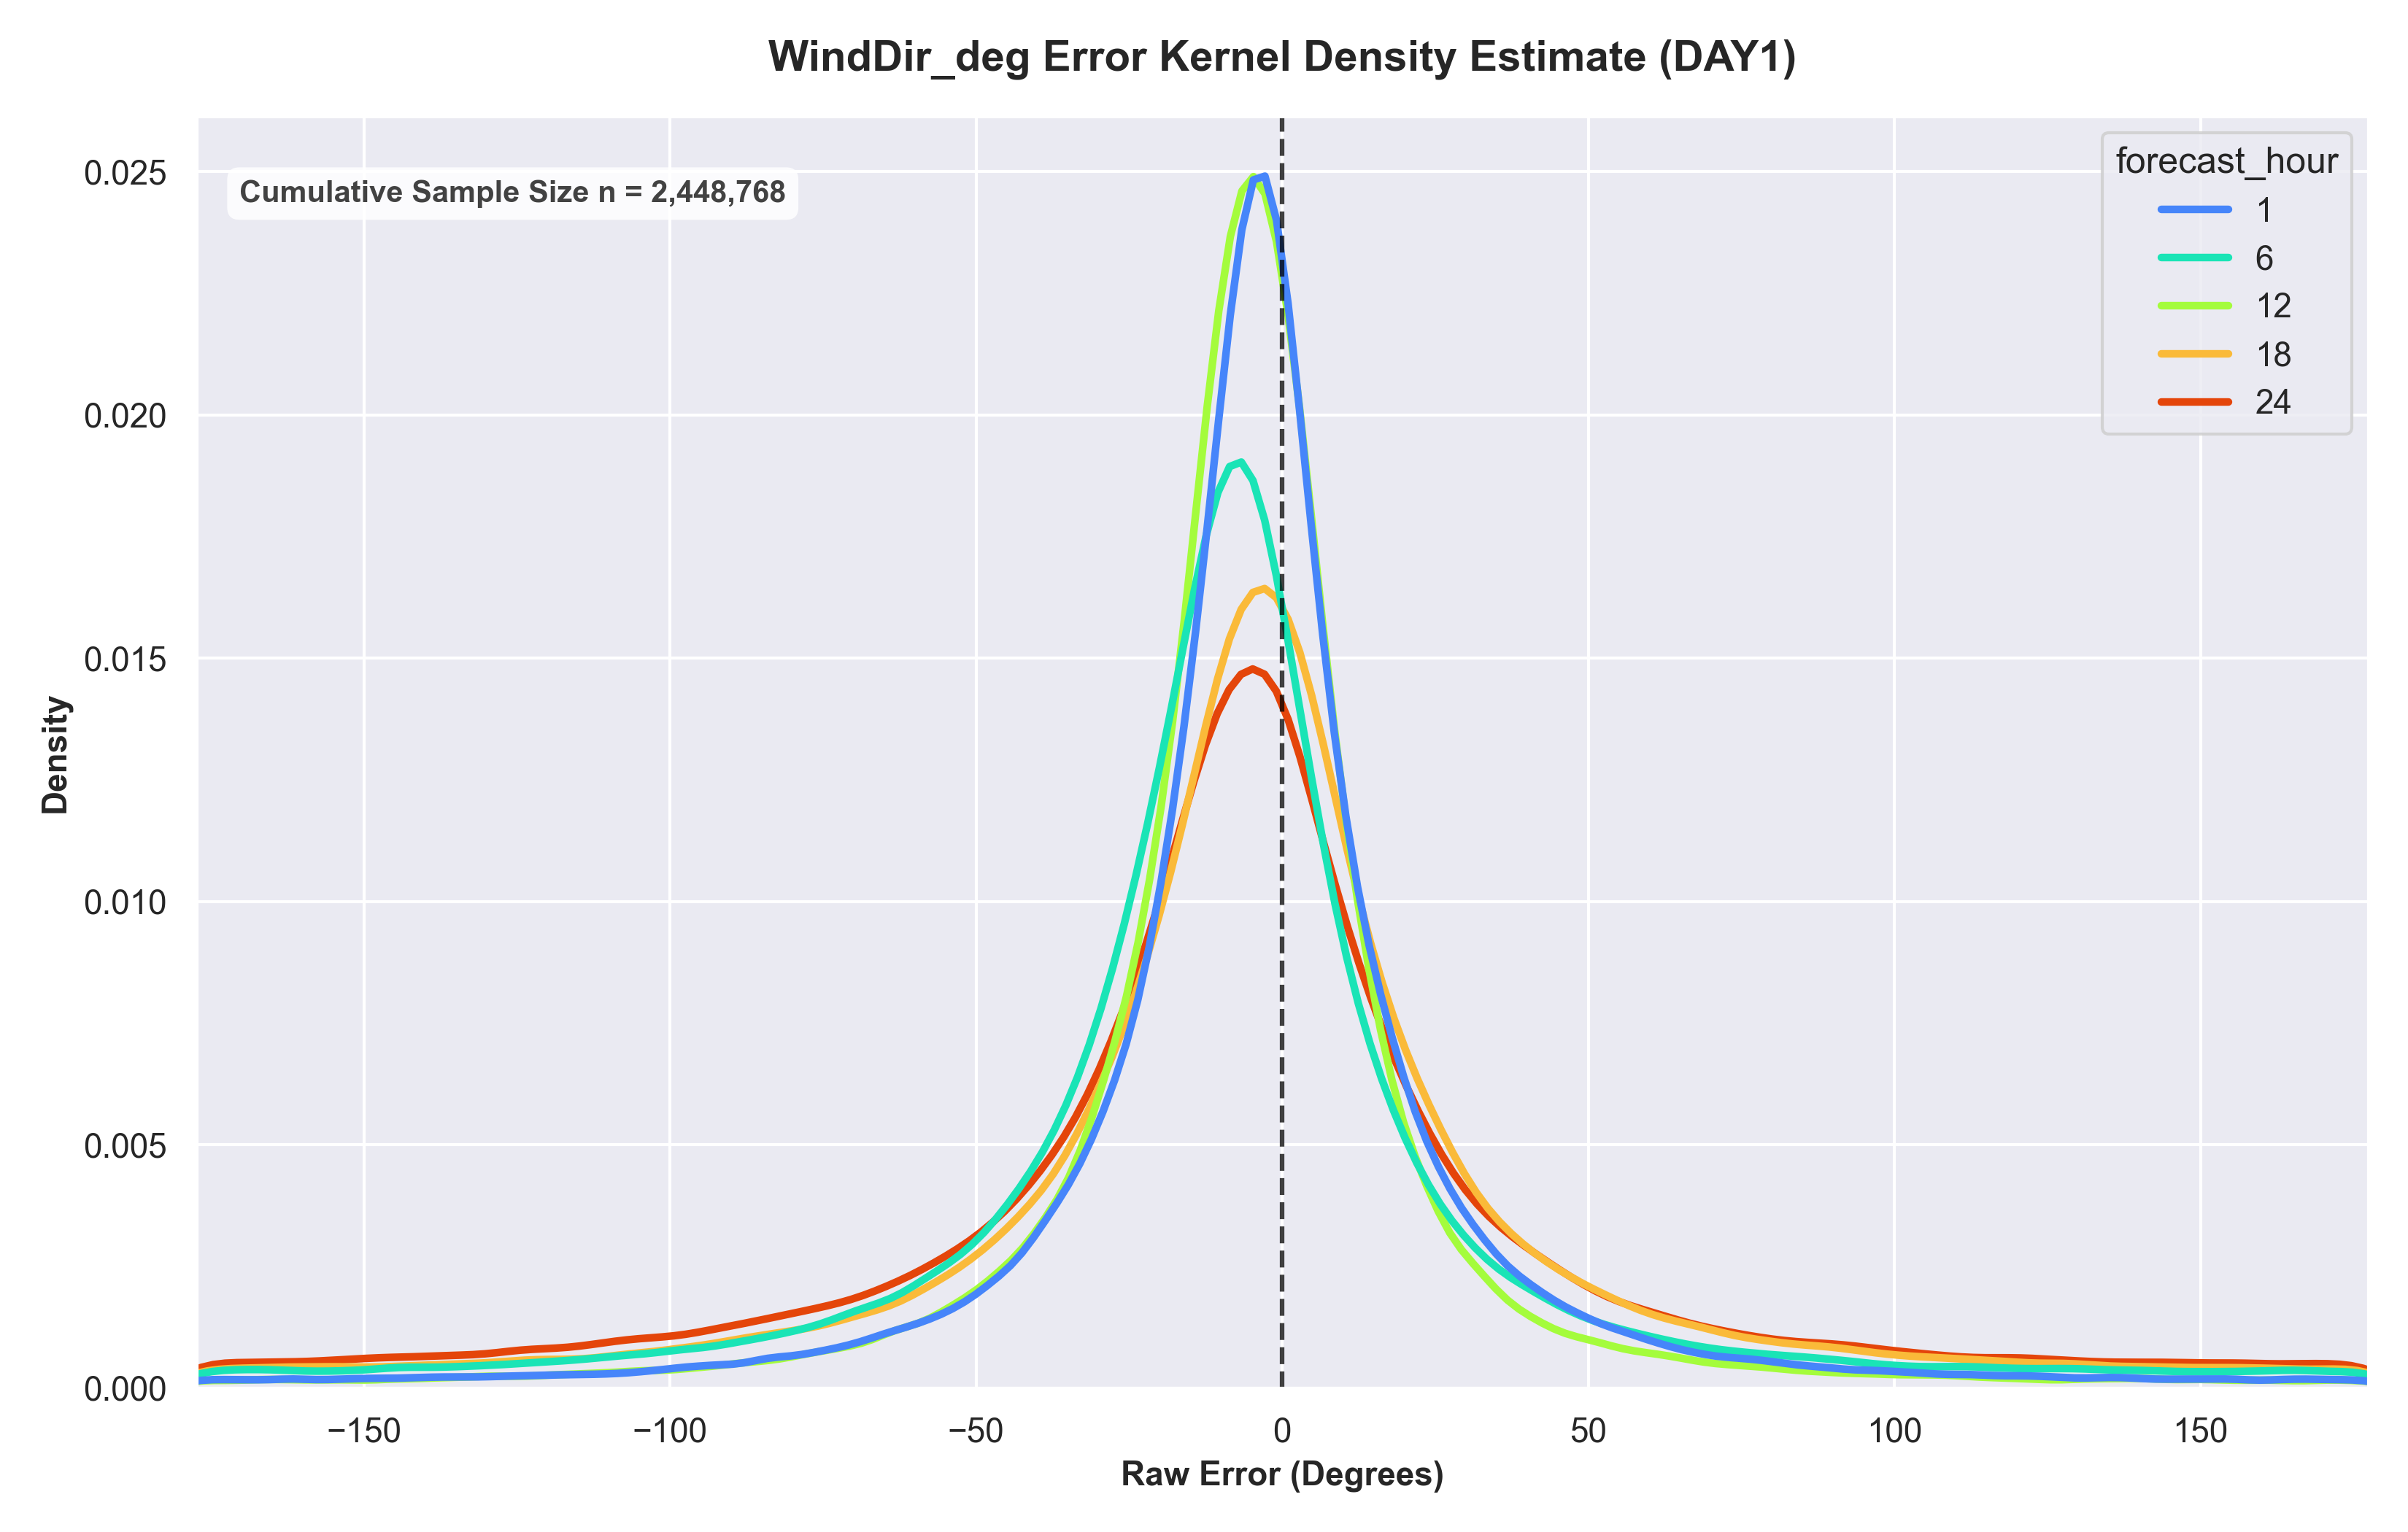
\includegraphics[width=0.49\textwidth]{figures/KDE_GRAPHS_RAW/winddir_deg_kde_day1.png}\hfill
  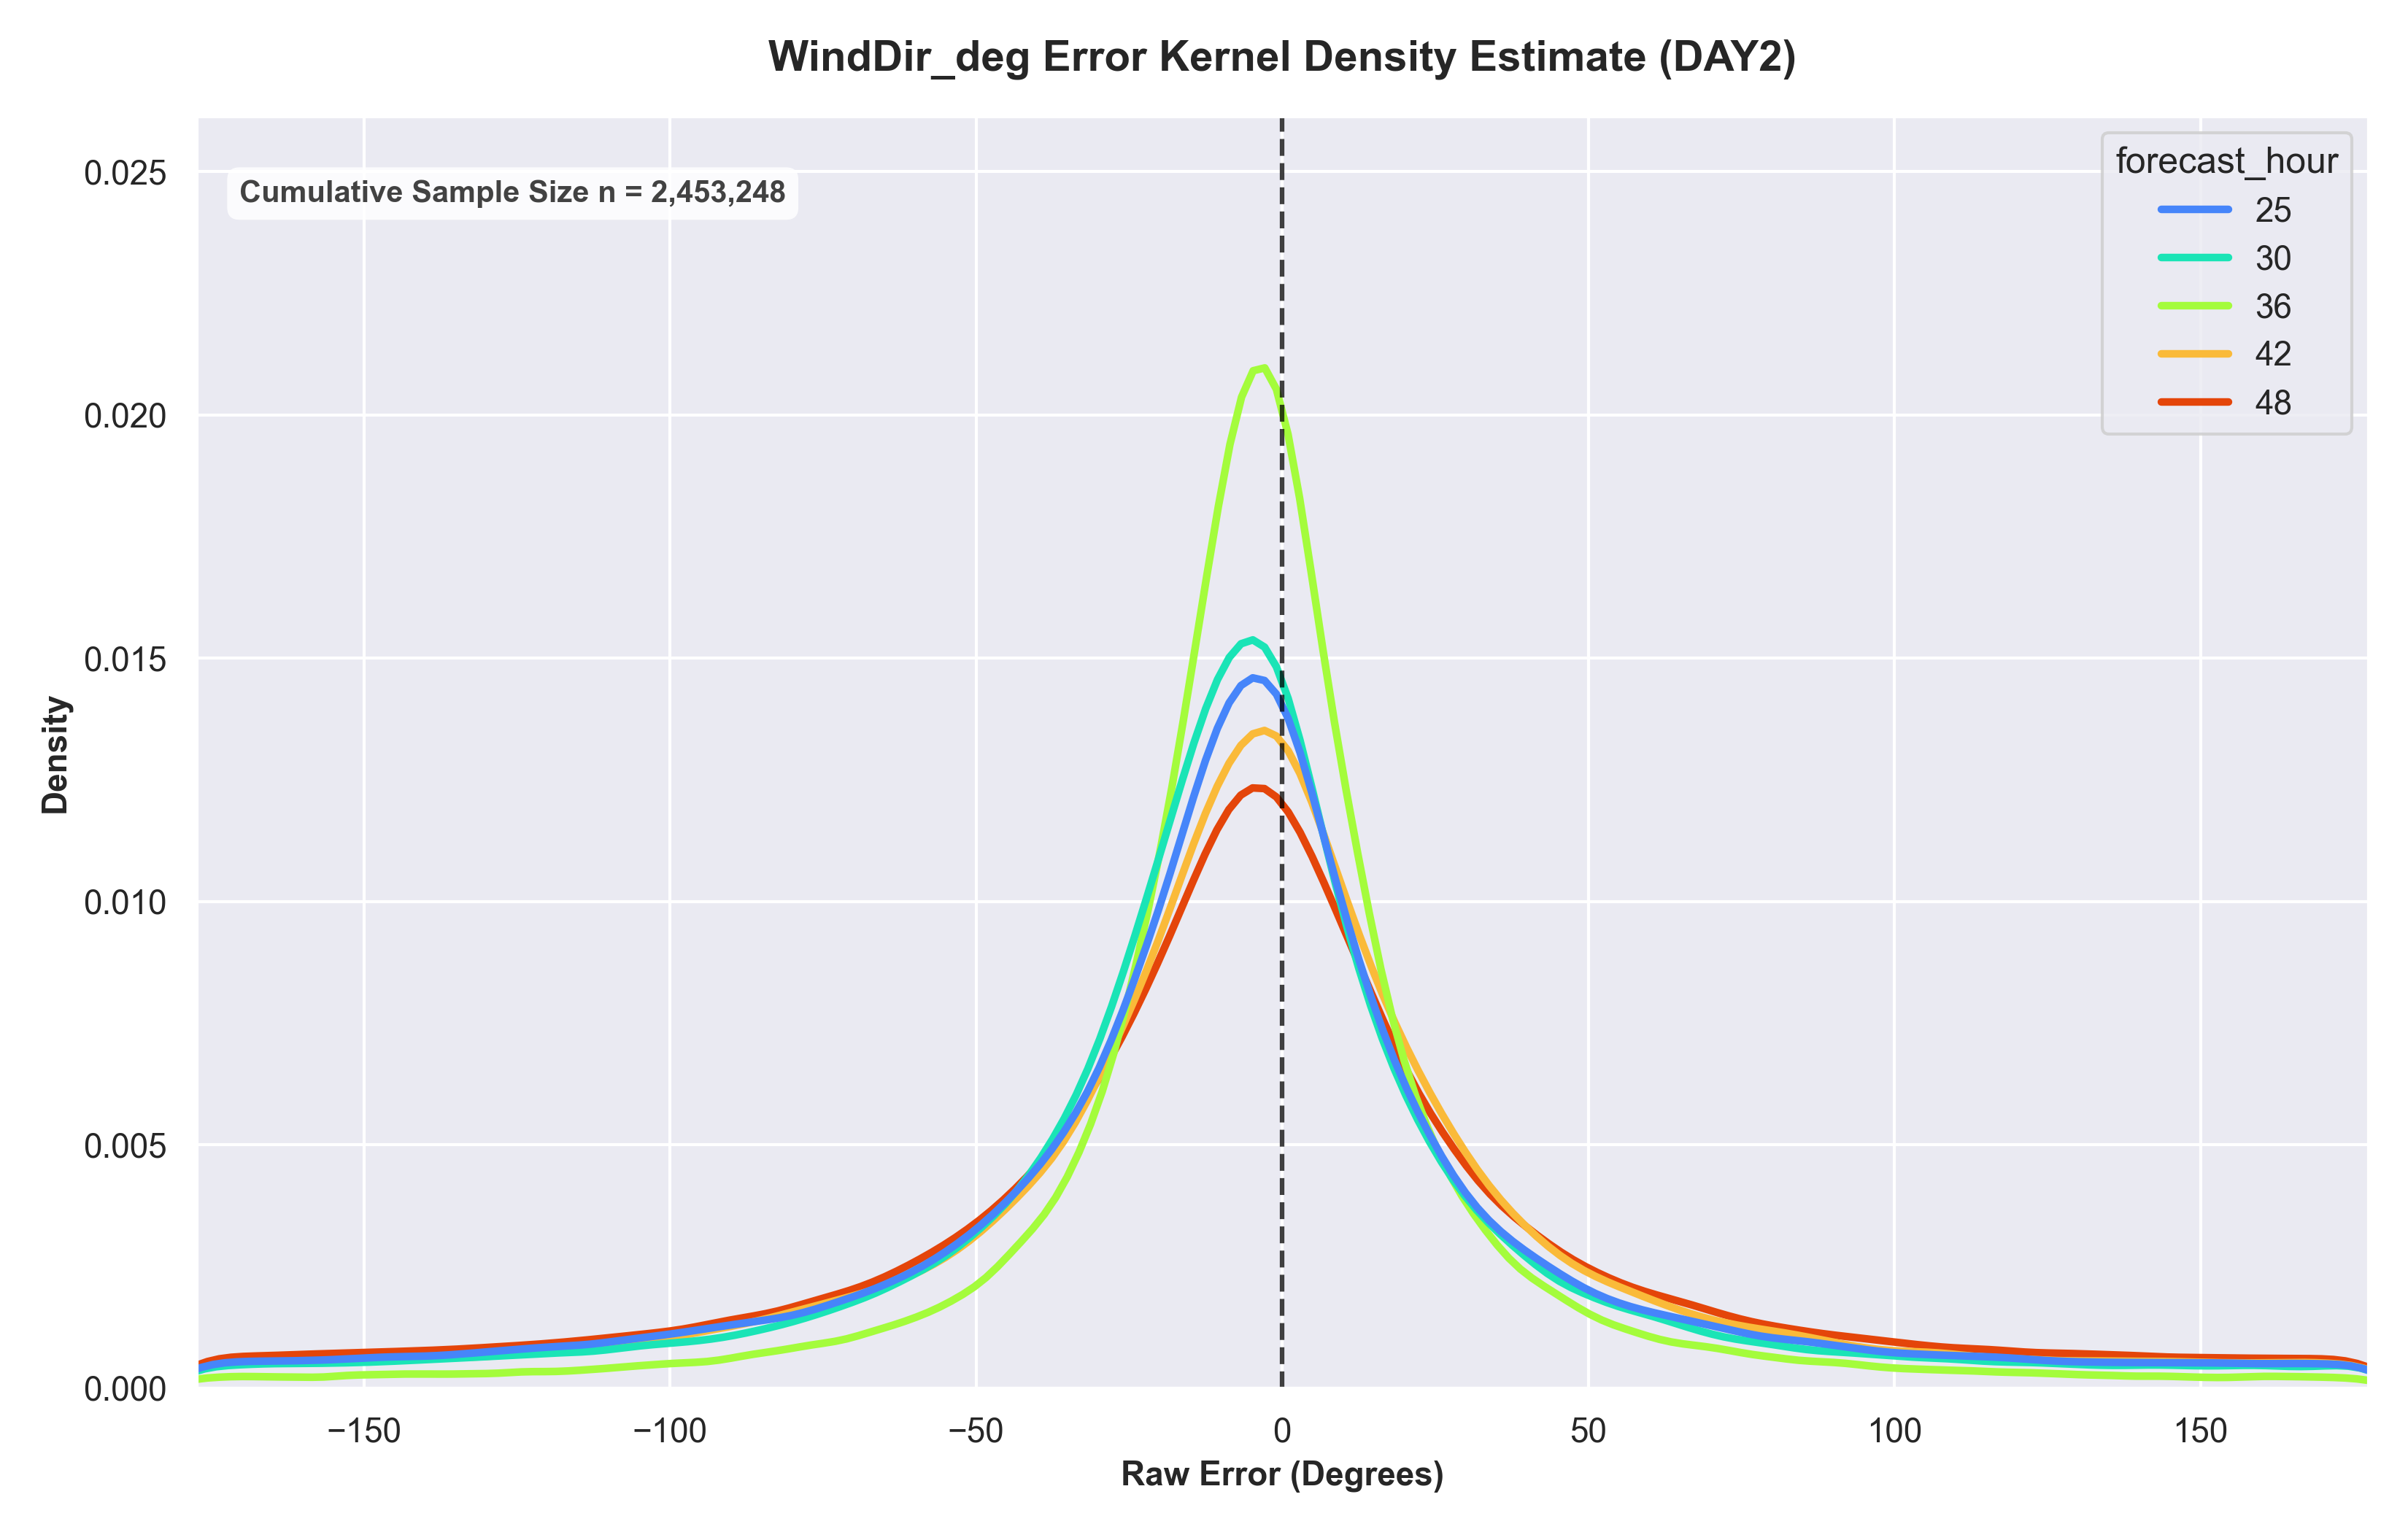
\includegraphics[width=0.49\textwidth]{figures/KDE_GRAPHS_RAW/winddir_deg_kde_day2.png}
  \caption{Kernel Density Estimation (KDE) of Wind Direction forecast errors for Day 1 (left) and Day 2 (right).}
  \label{fig:kde_winddir}
\end{figure}

\subsection{Q2 — Forecast Error vs. Lead Time}

\begin{figure}[H]
  \centering
  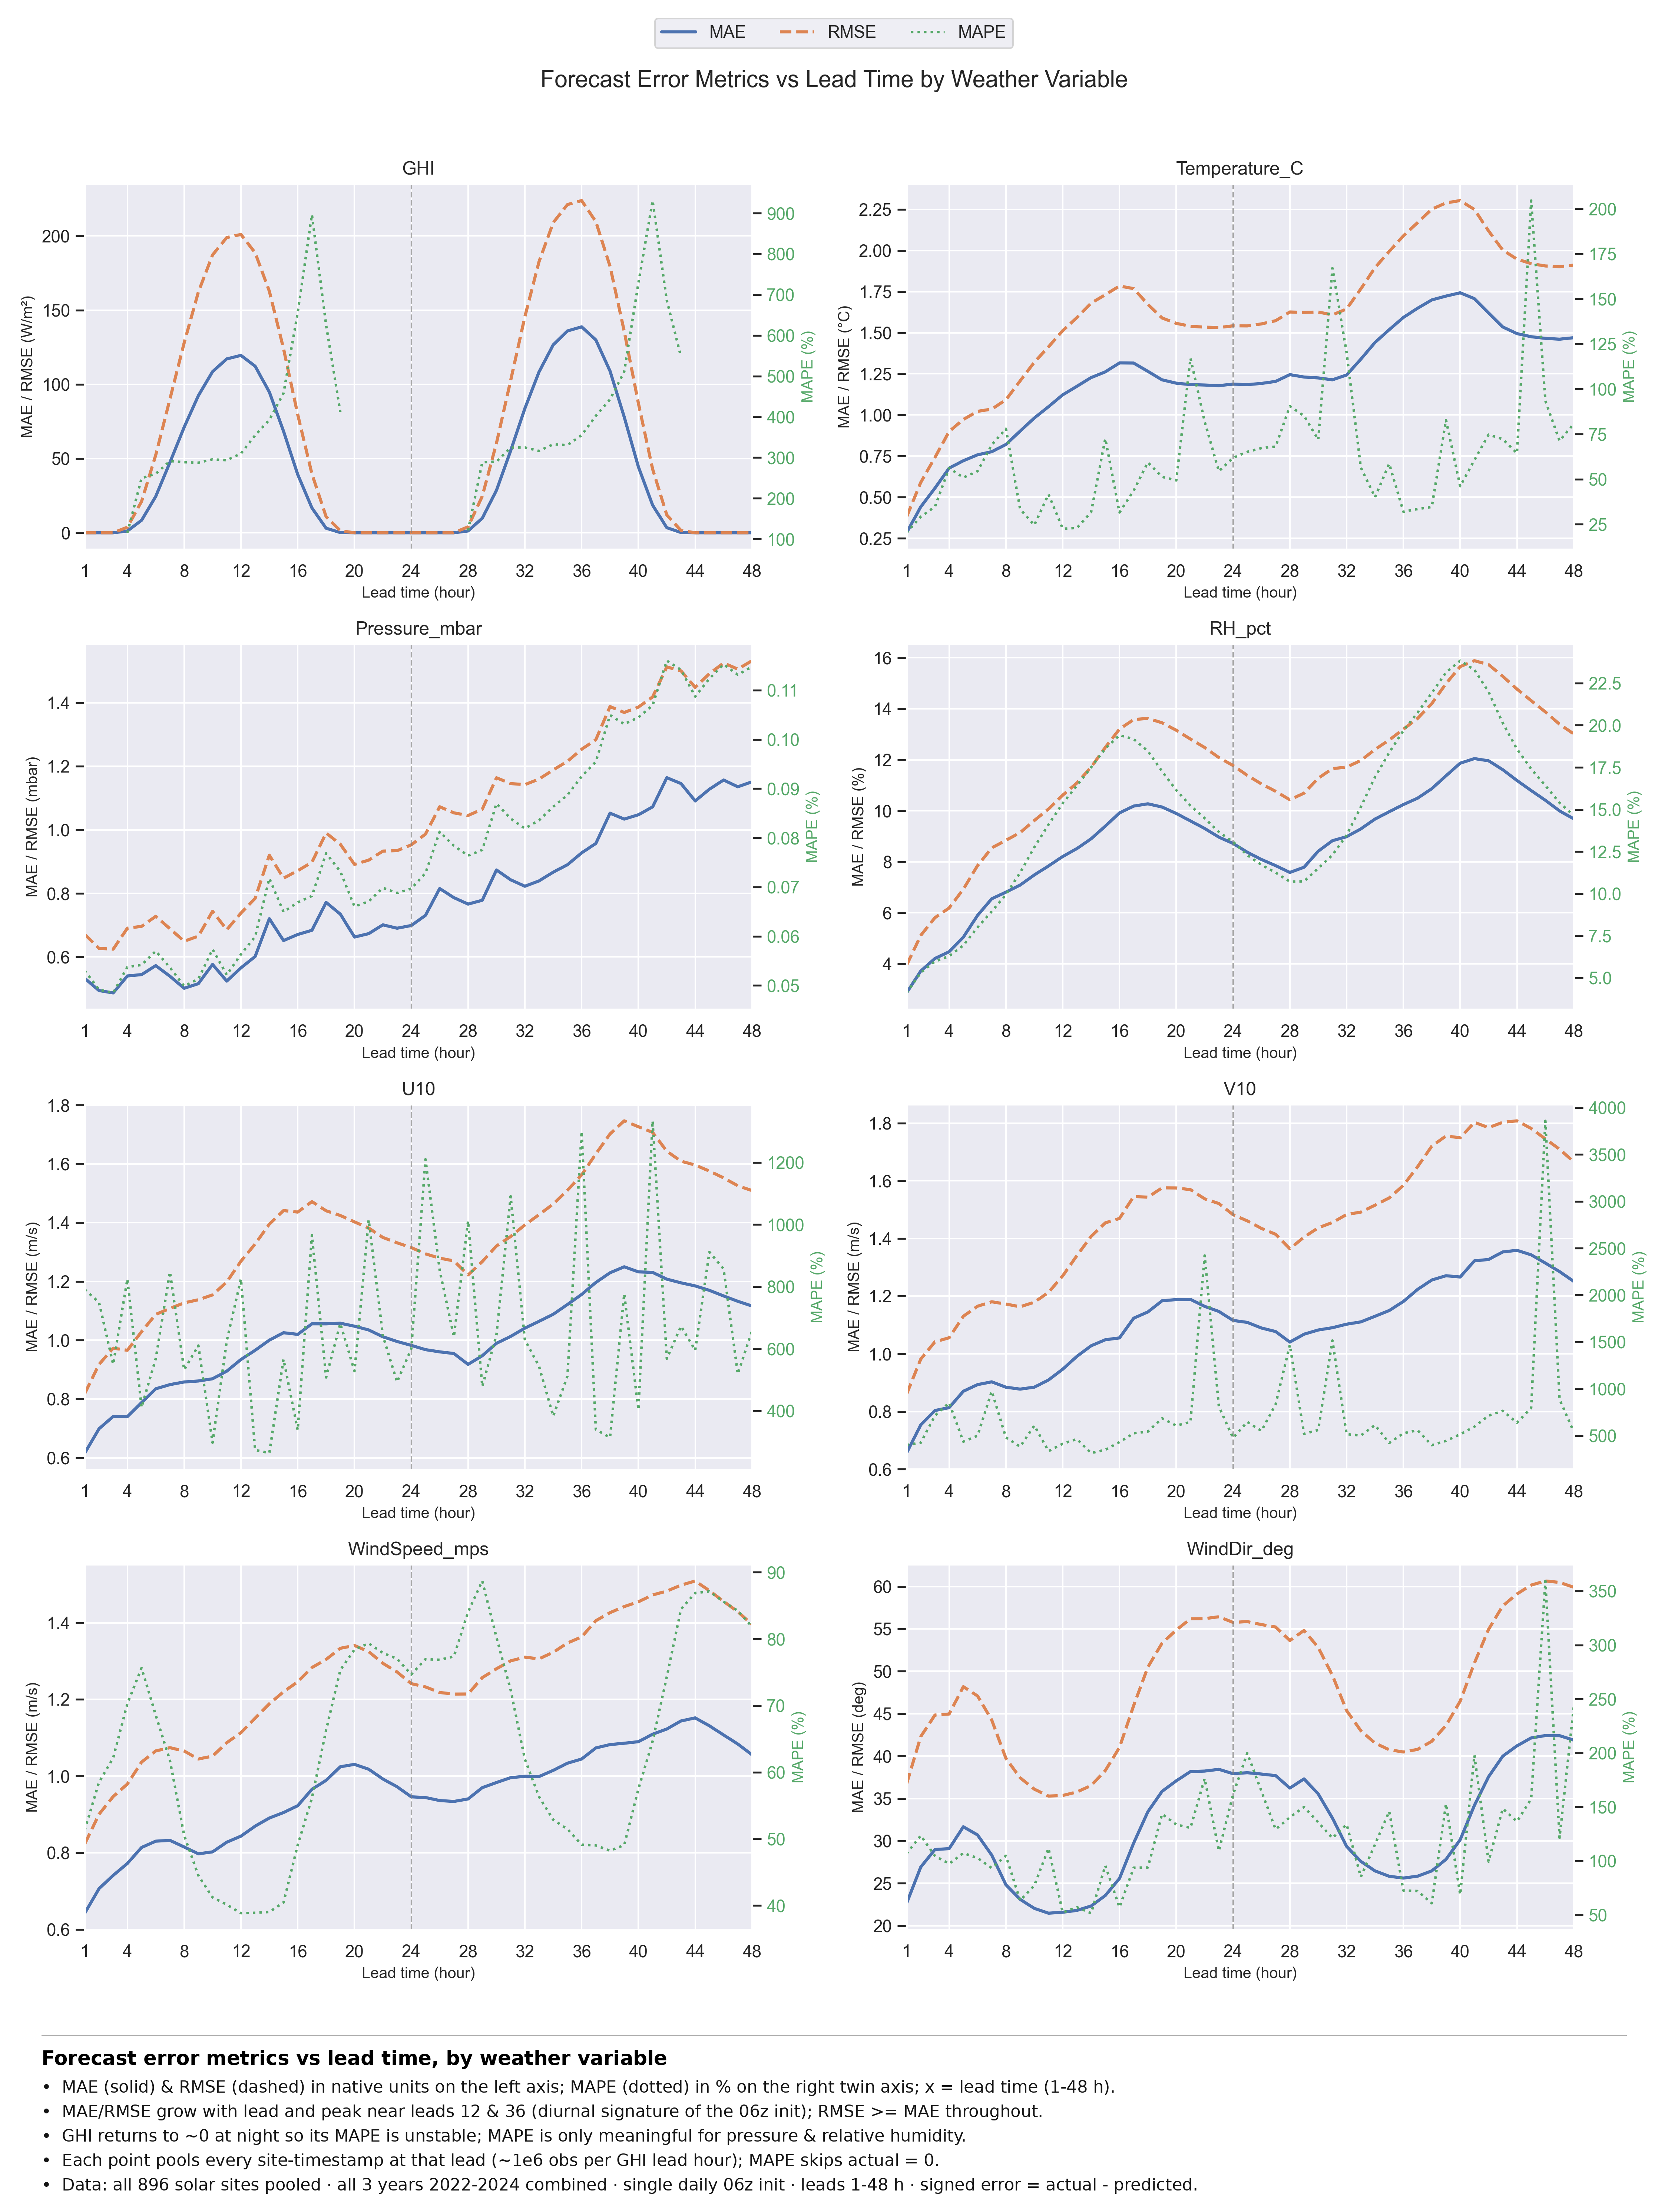
\includegraphics[width=\textwidth]{figures/Q2/error_by_lead_time_solar.png}
  \caption{Complete (all-variable) version of forecast error metrics versus lead time.}
  \label{fig:app_leadtime}
\end{figure}

\begin{figure}[H]
  \centering
  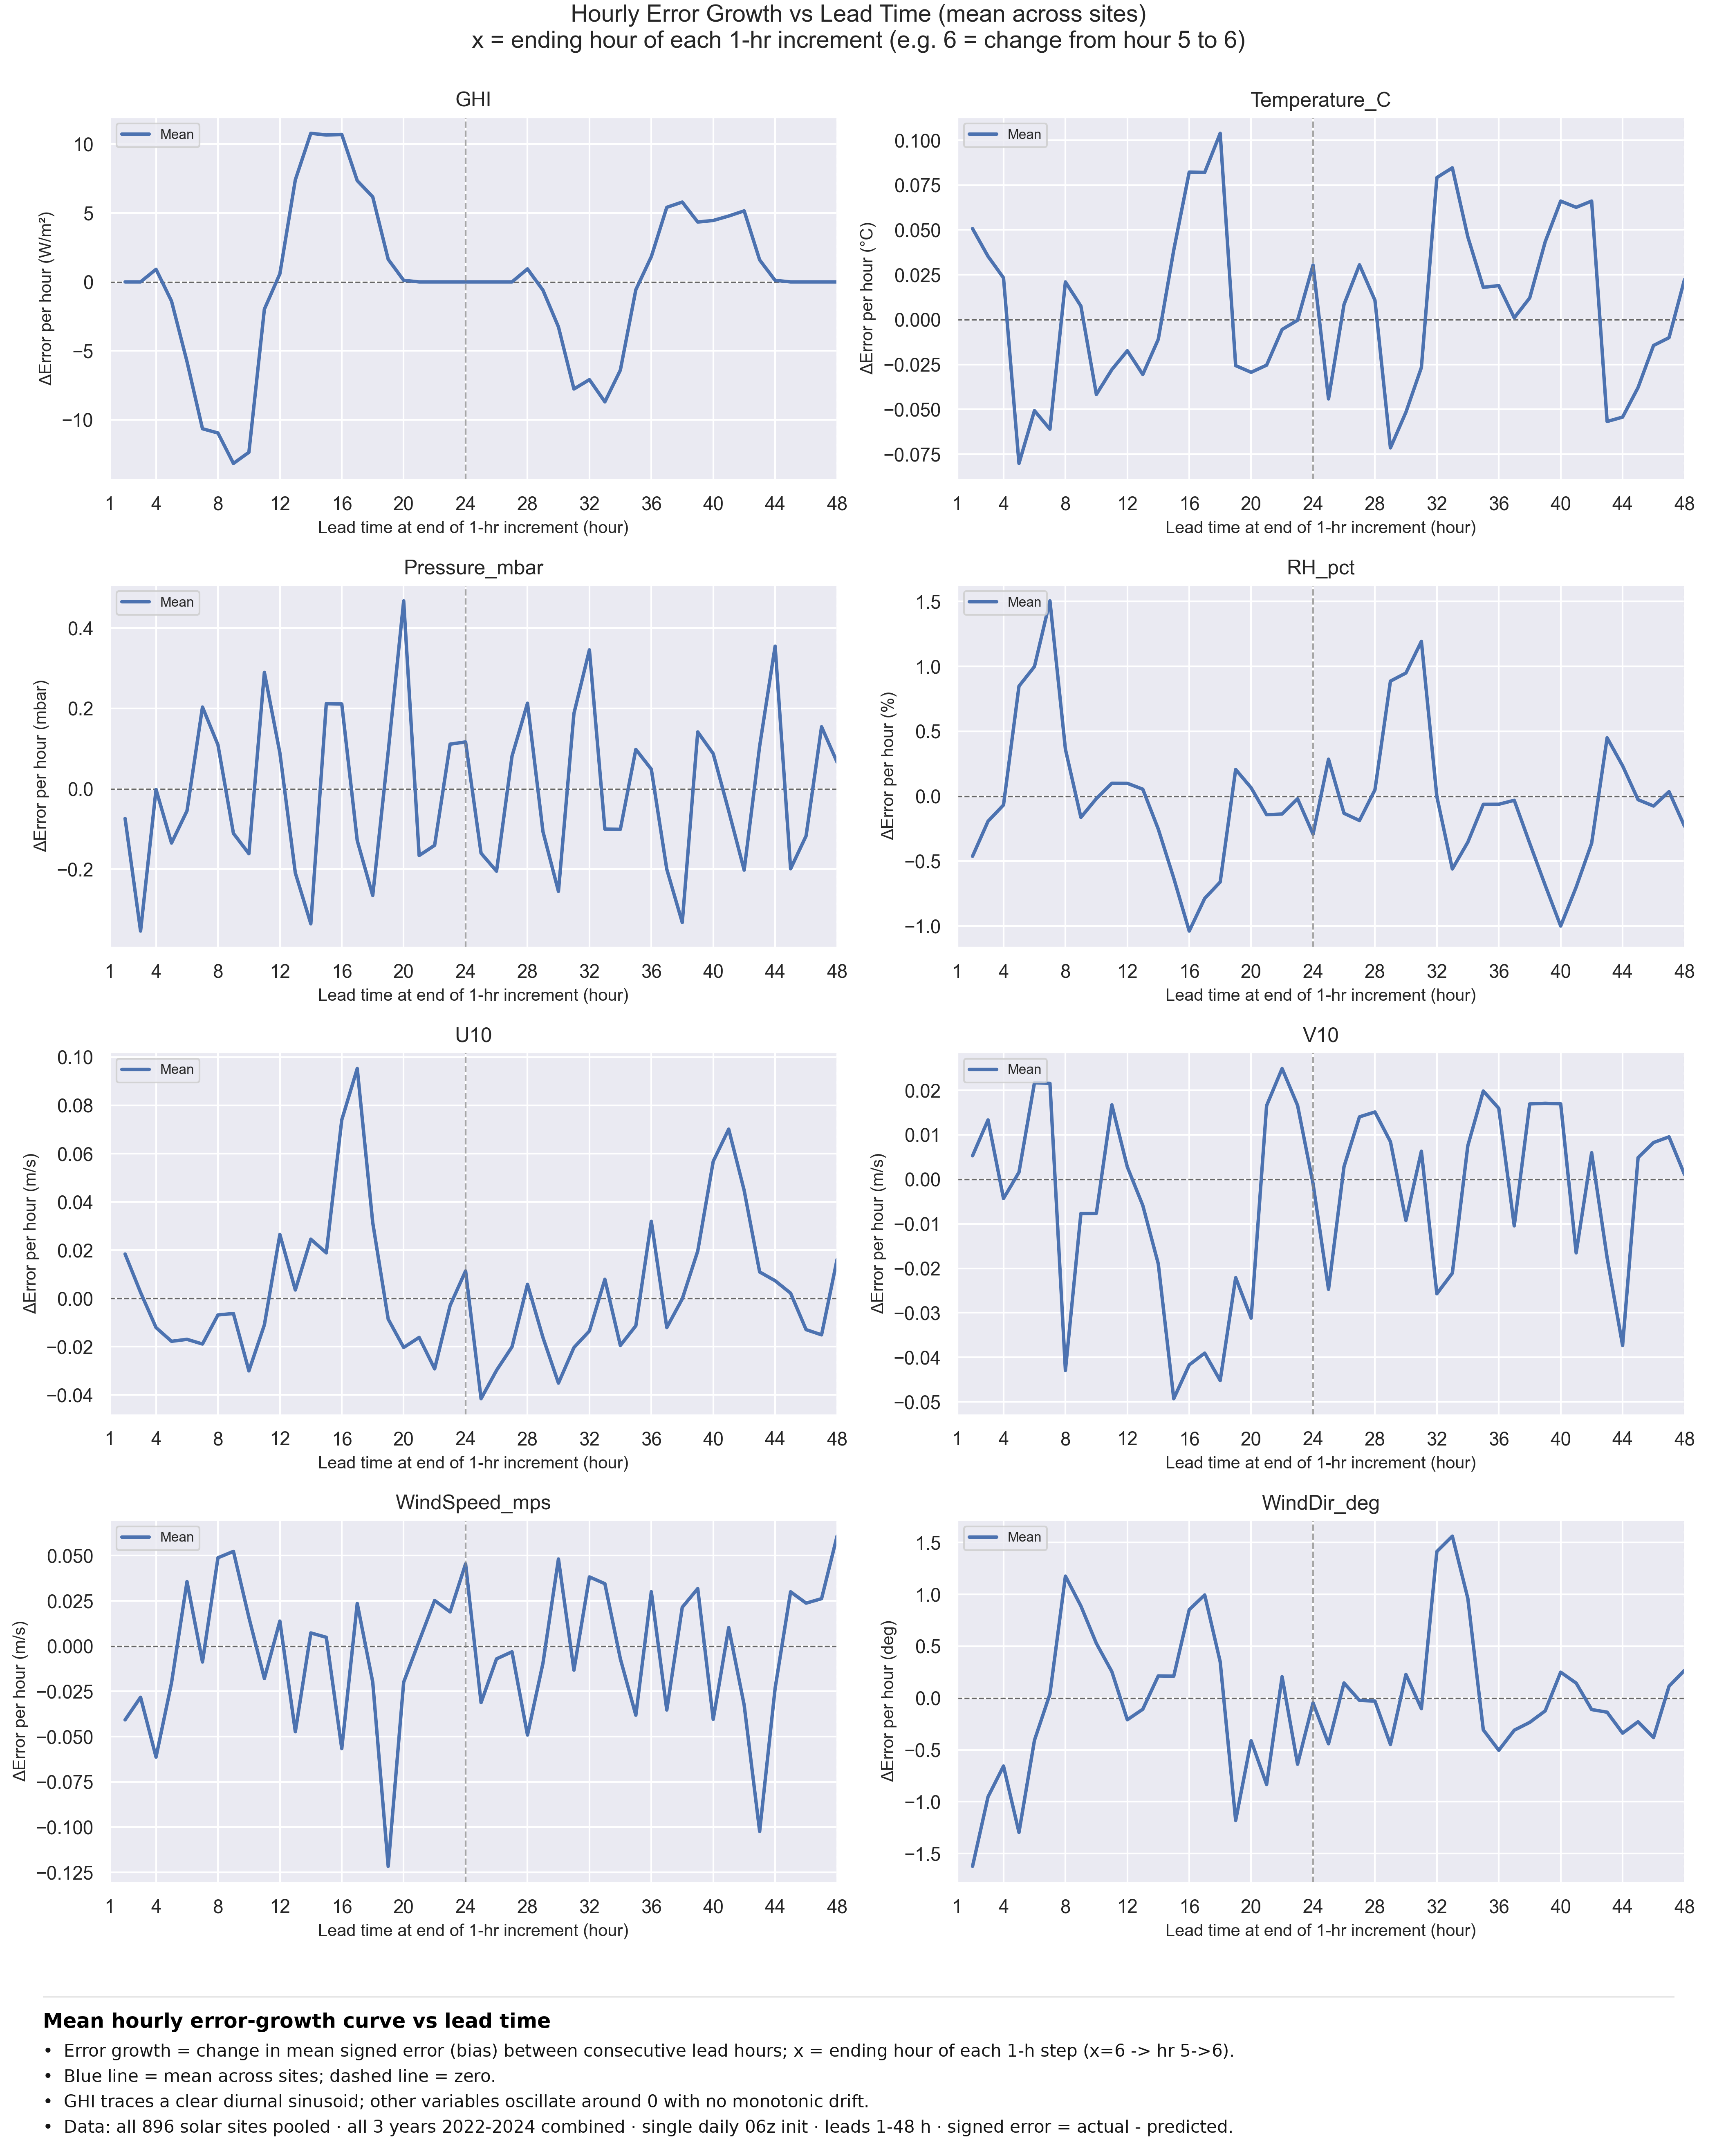
\includegraphics[width=\textwidth]{figures/Q2/error_growth_curves.png}
  \caption{Complete (all-variable) version of the fleet-mean hourly error-growth curves.}
  \label{fig:app_growthcurves}
\end{figure}

\begin{figure}[H]
  \centering
  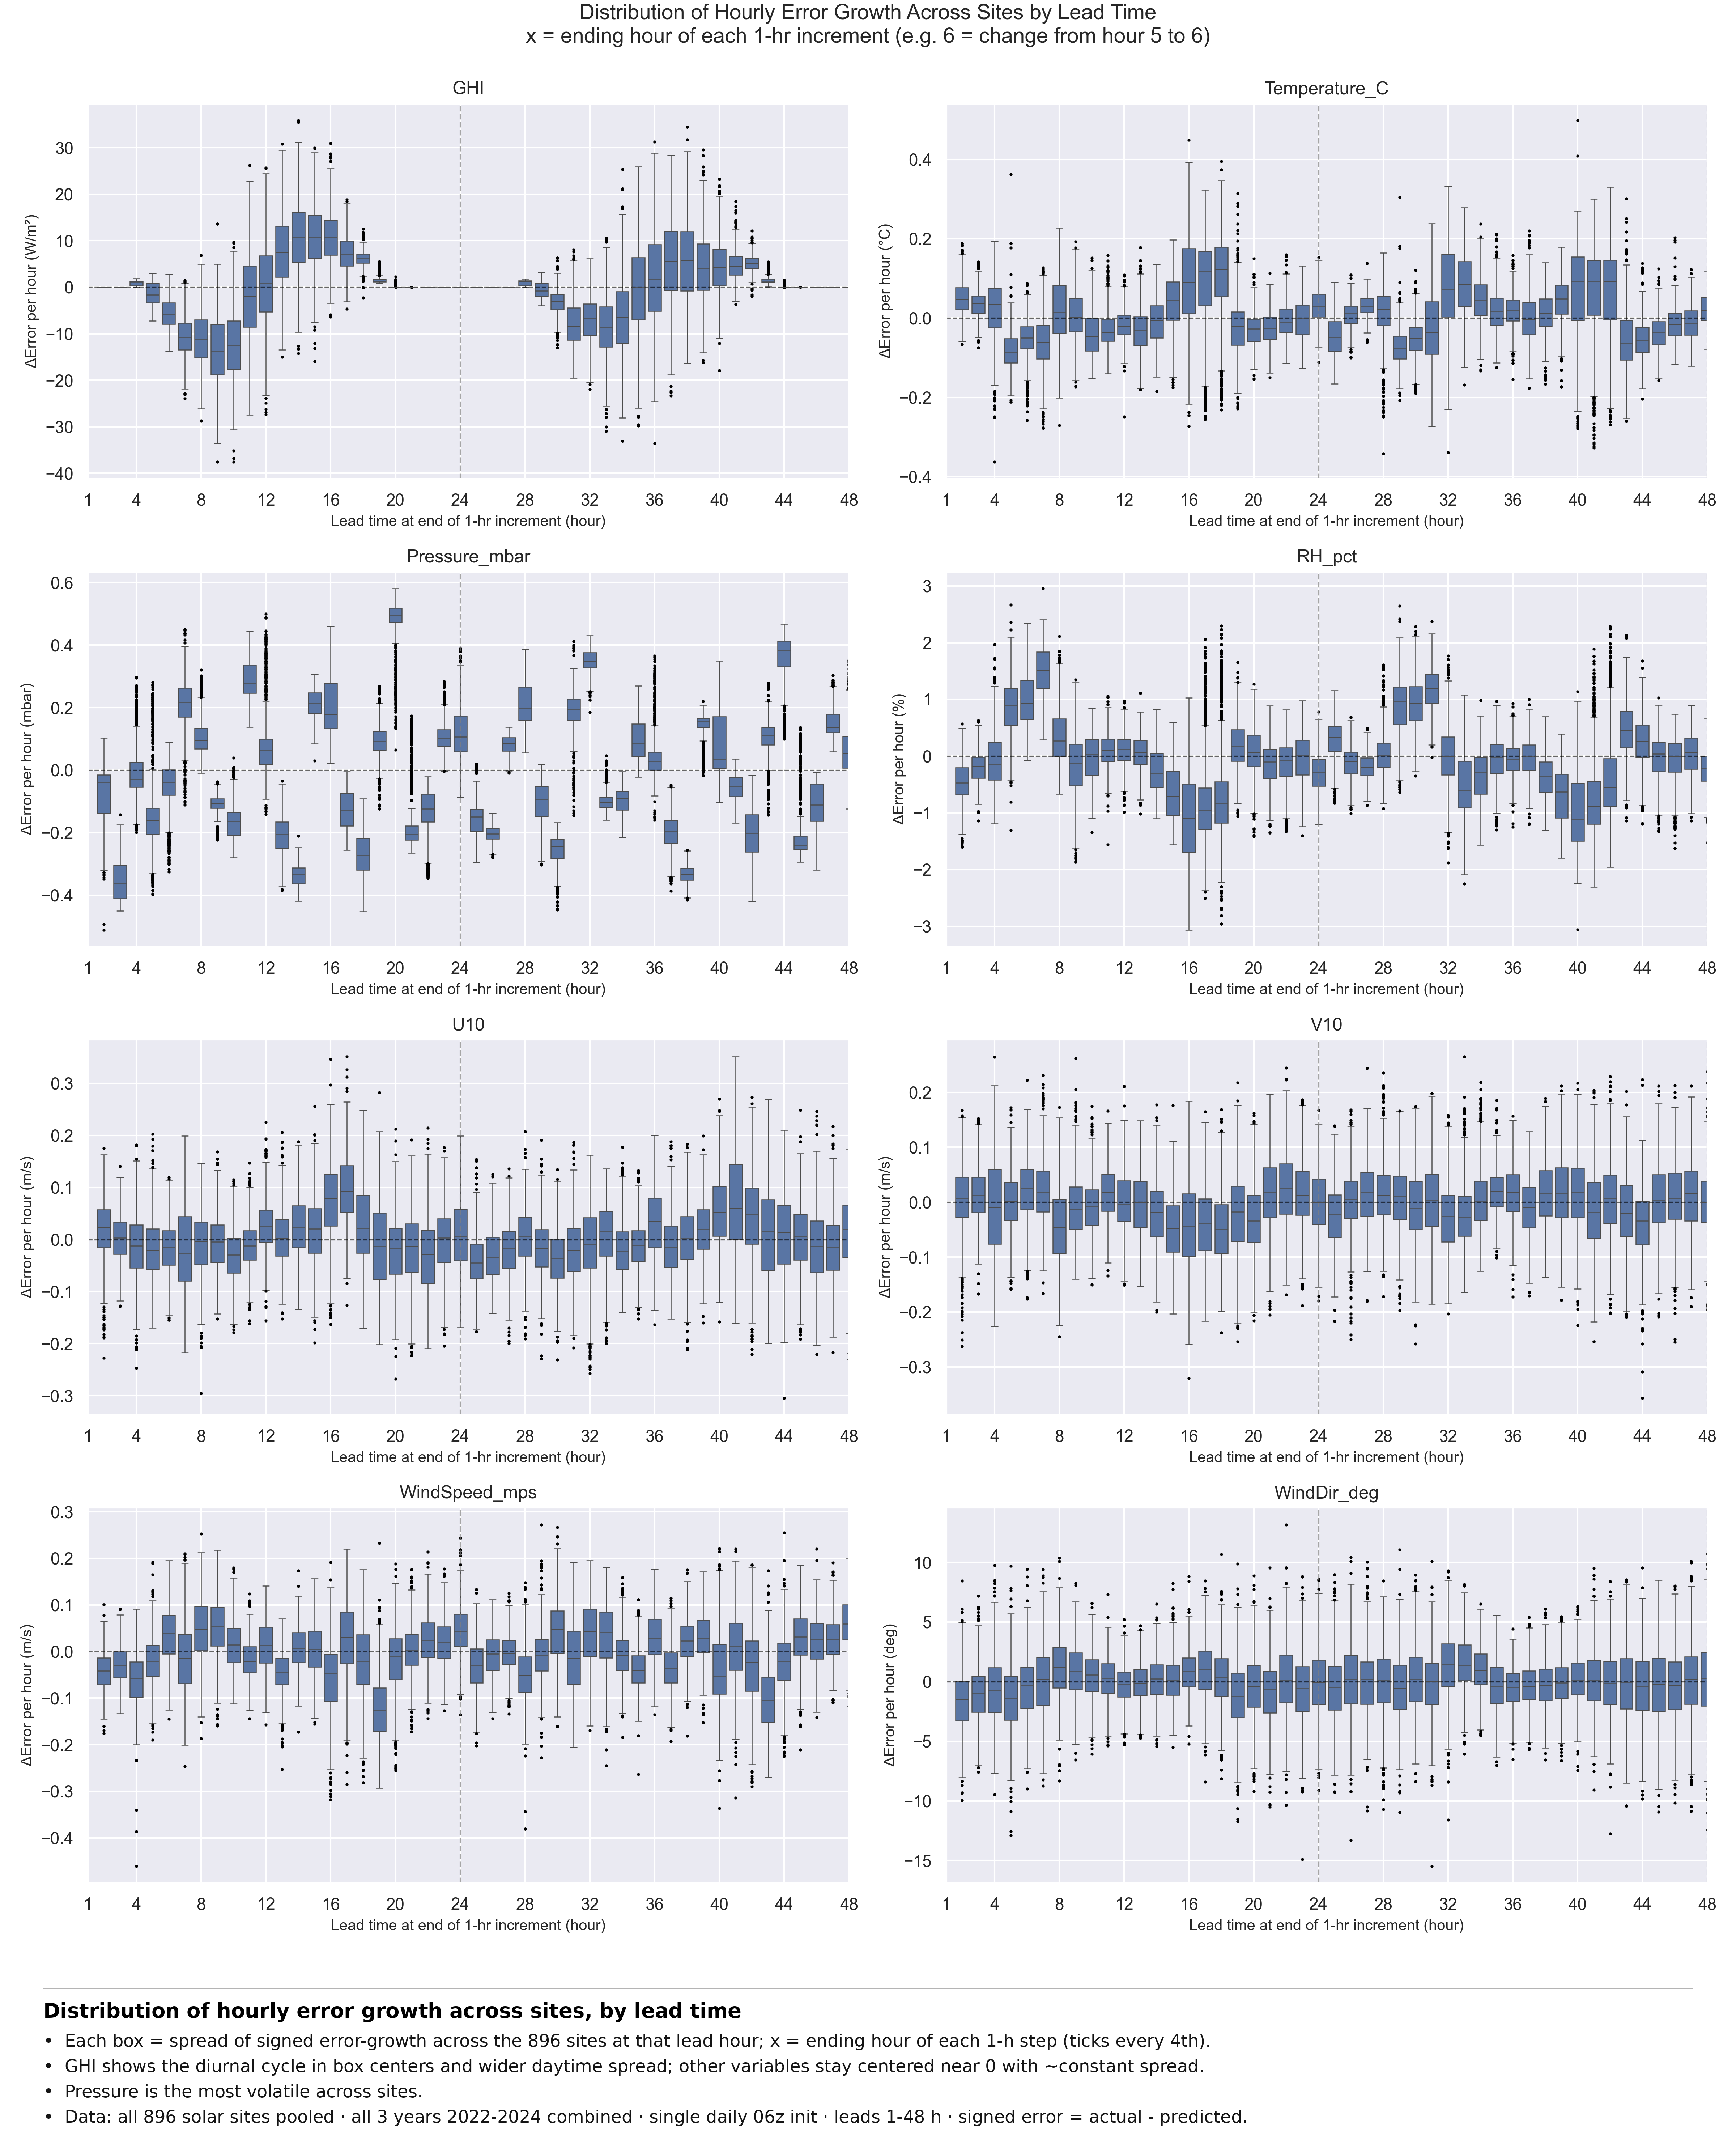
\includegraphics[width=\textwidth]{figures/Q2/error_growth_distributions.png}
  \caption{Complete (all-variable) version of the hourly error-growth distributions across sites.}
  \label{fig:app_growthdist}
\end{figure}

\begin{figure}[H]
  \centering
  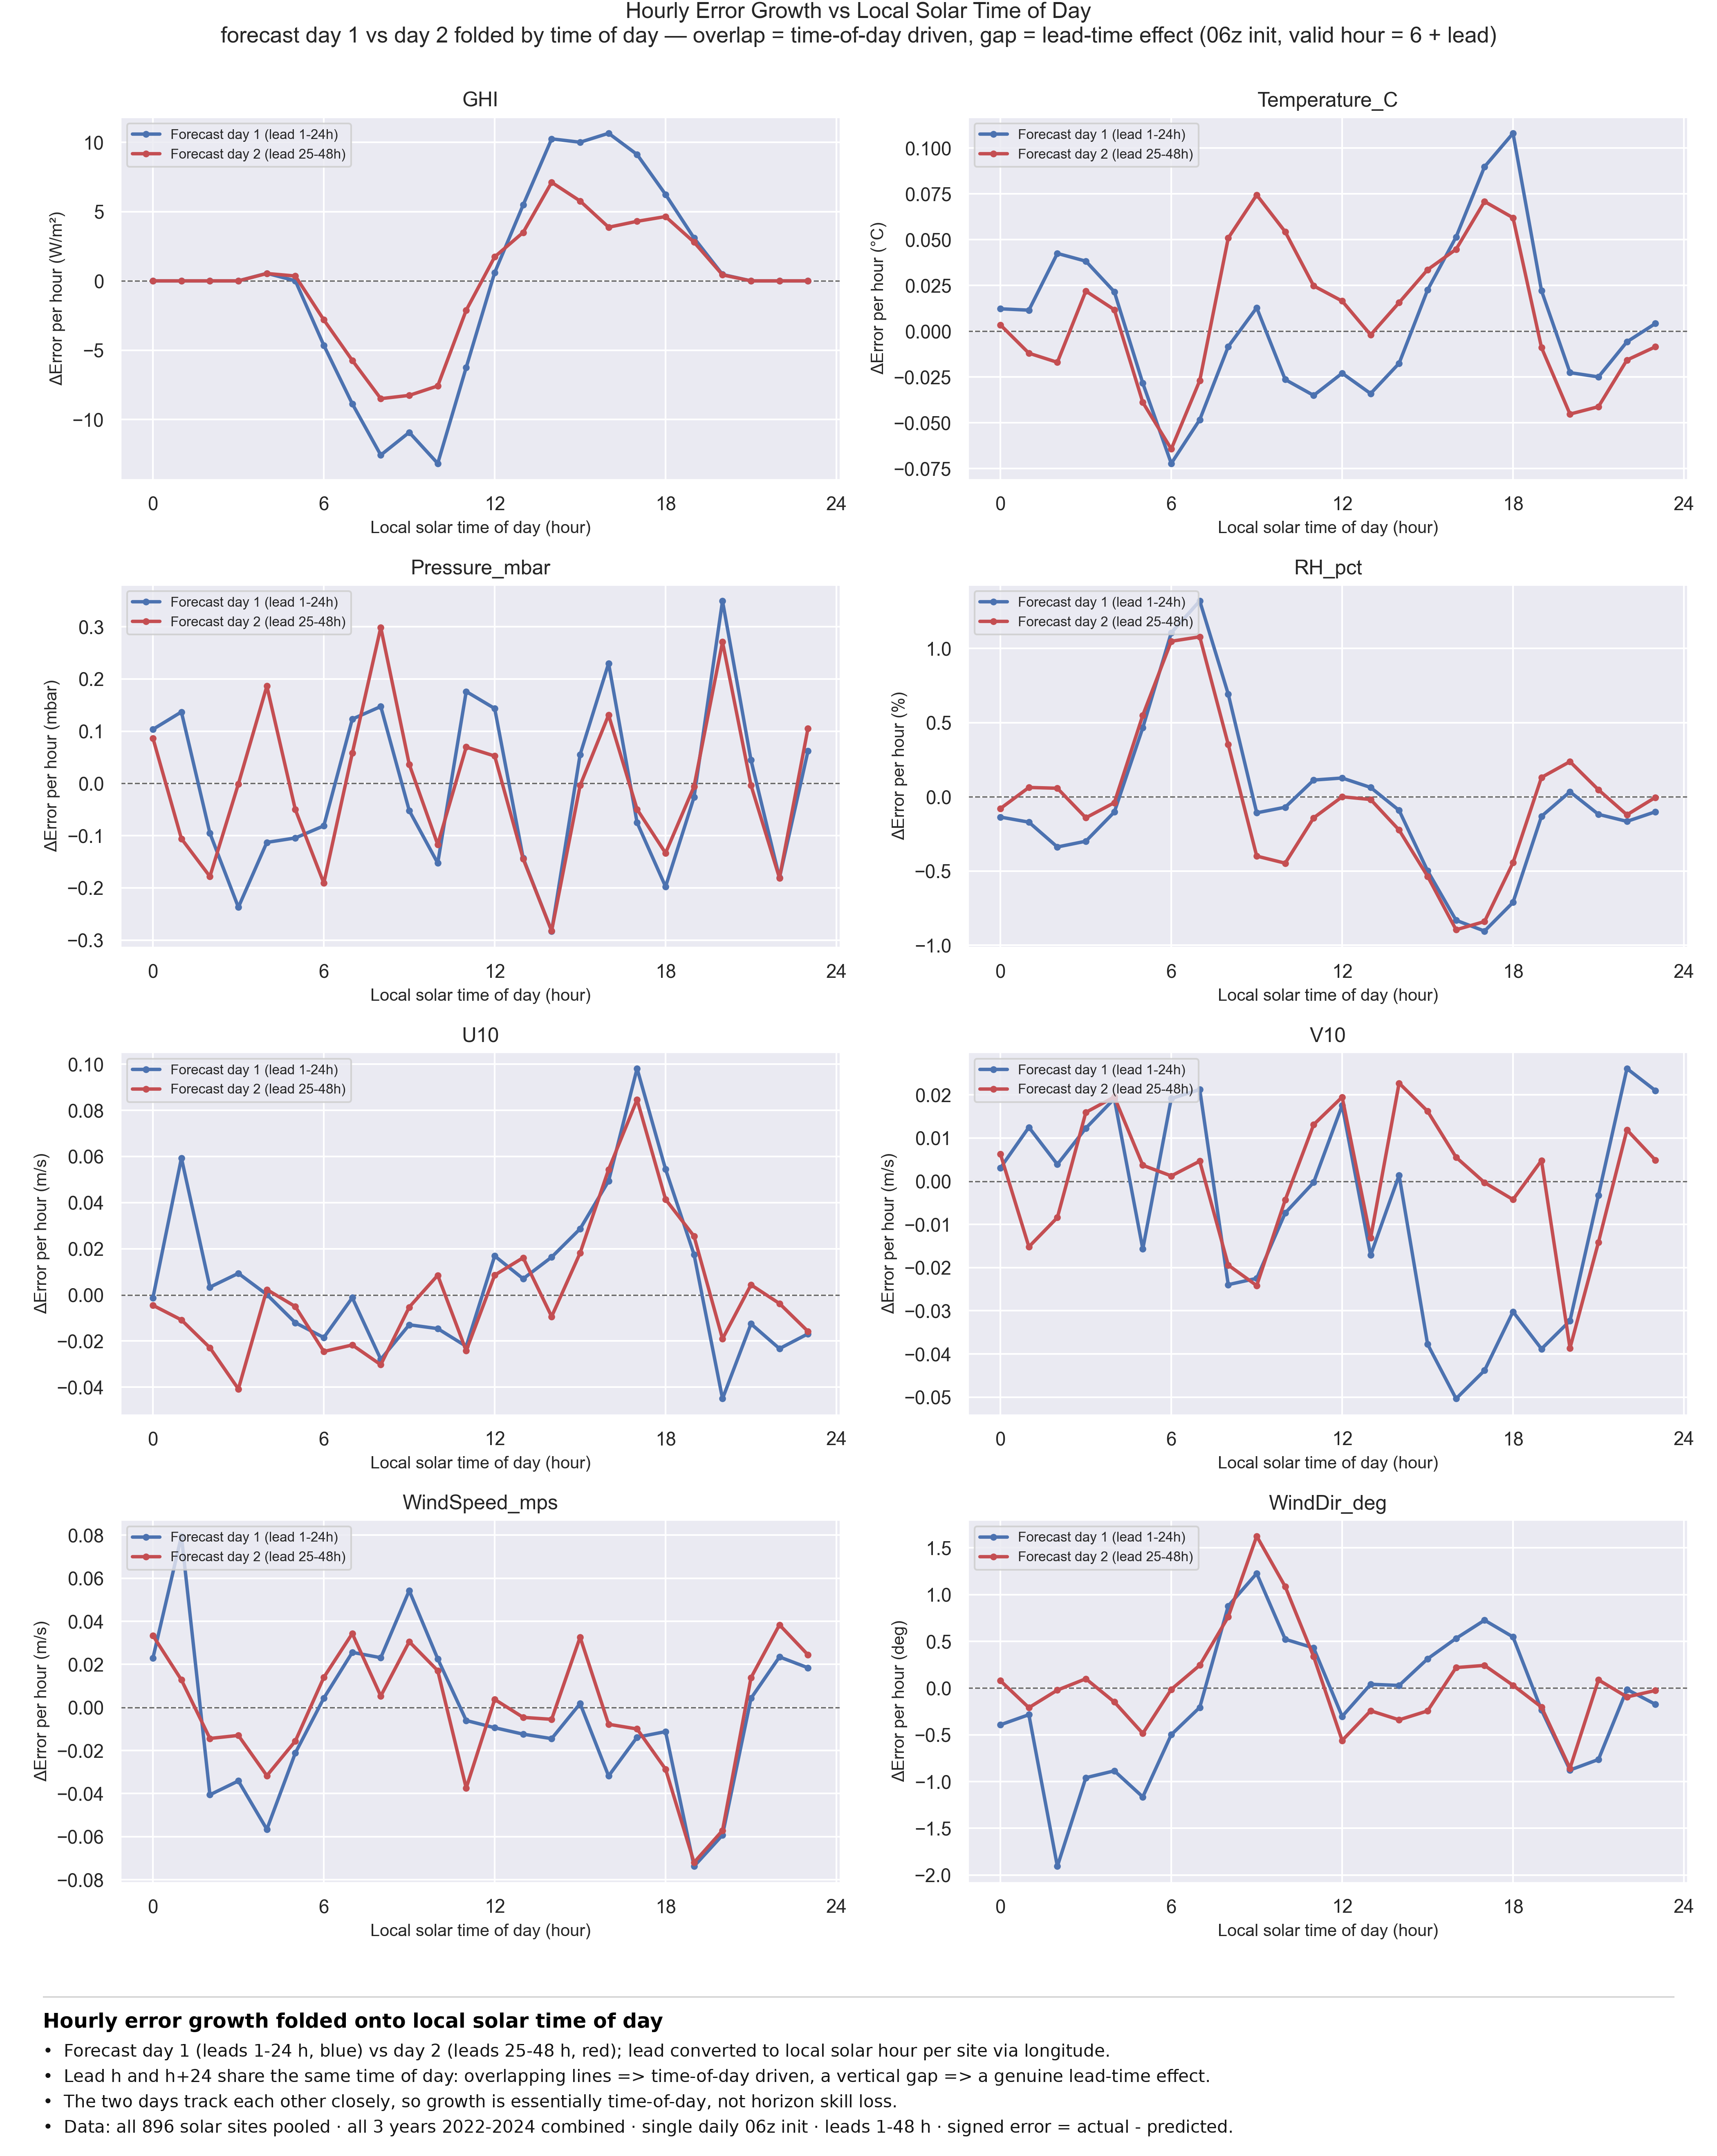
\includegraphics[width=\textwidth]{figures/Q2/error_growth_vs_time_of_day.png}
  \caption{Complete (all-variable) version of hourly error growth folded onto local solar time of day.}
  \label{fig:app_tod}
\end{figure}

\subsection{Q4 and Q5}

\begin{figure}[H]
    \centering
    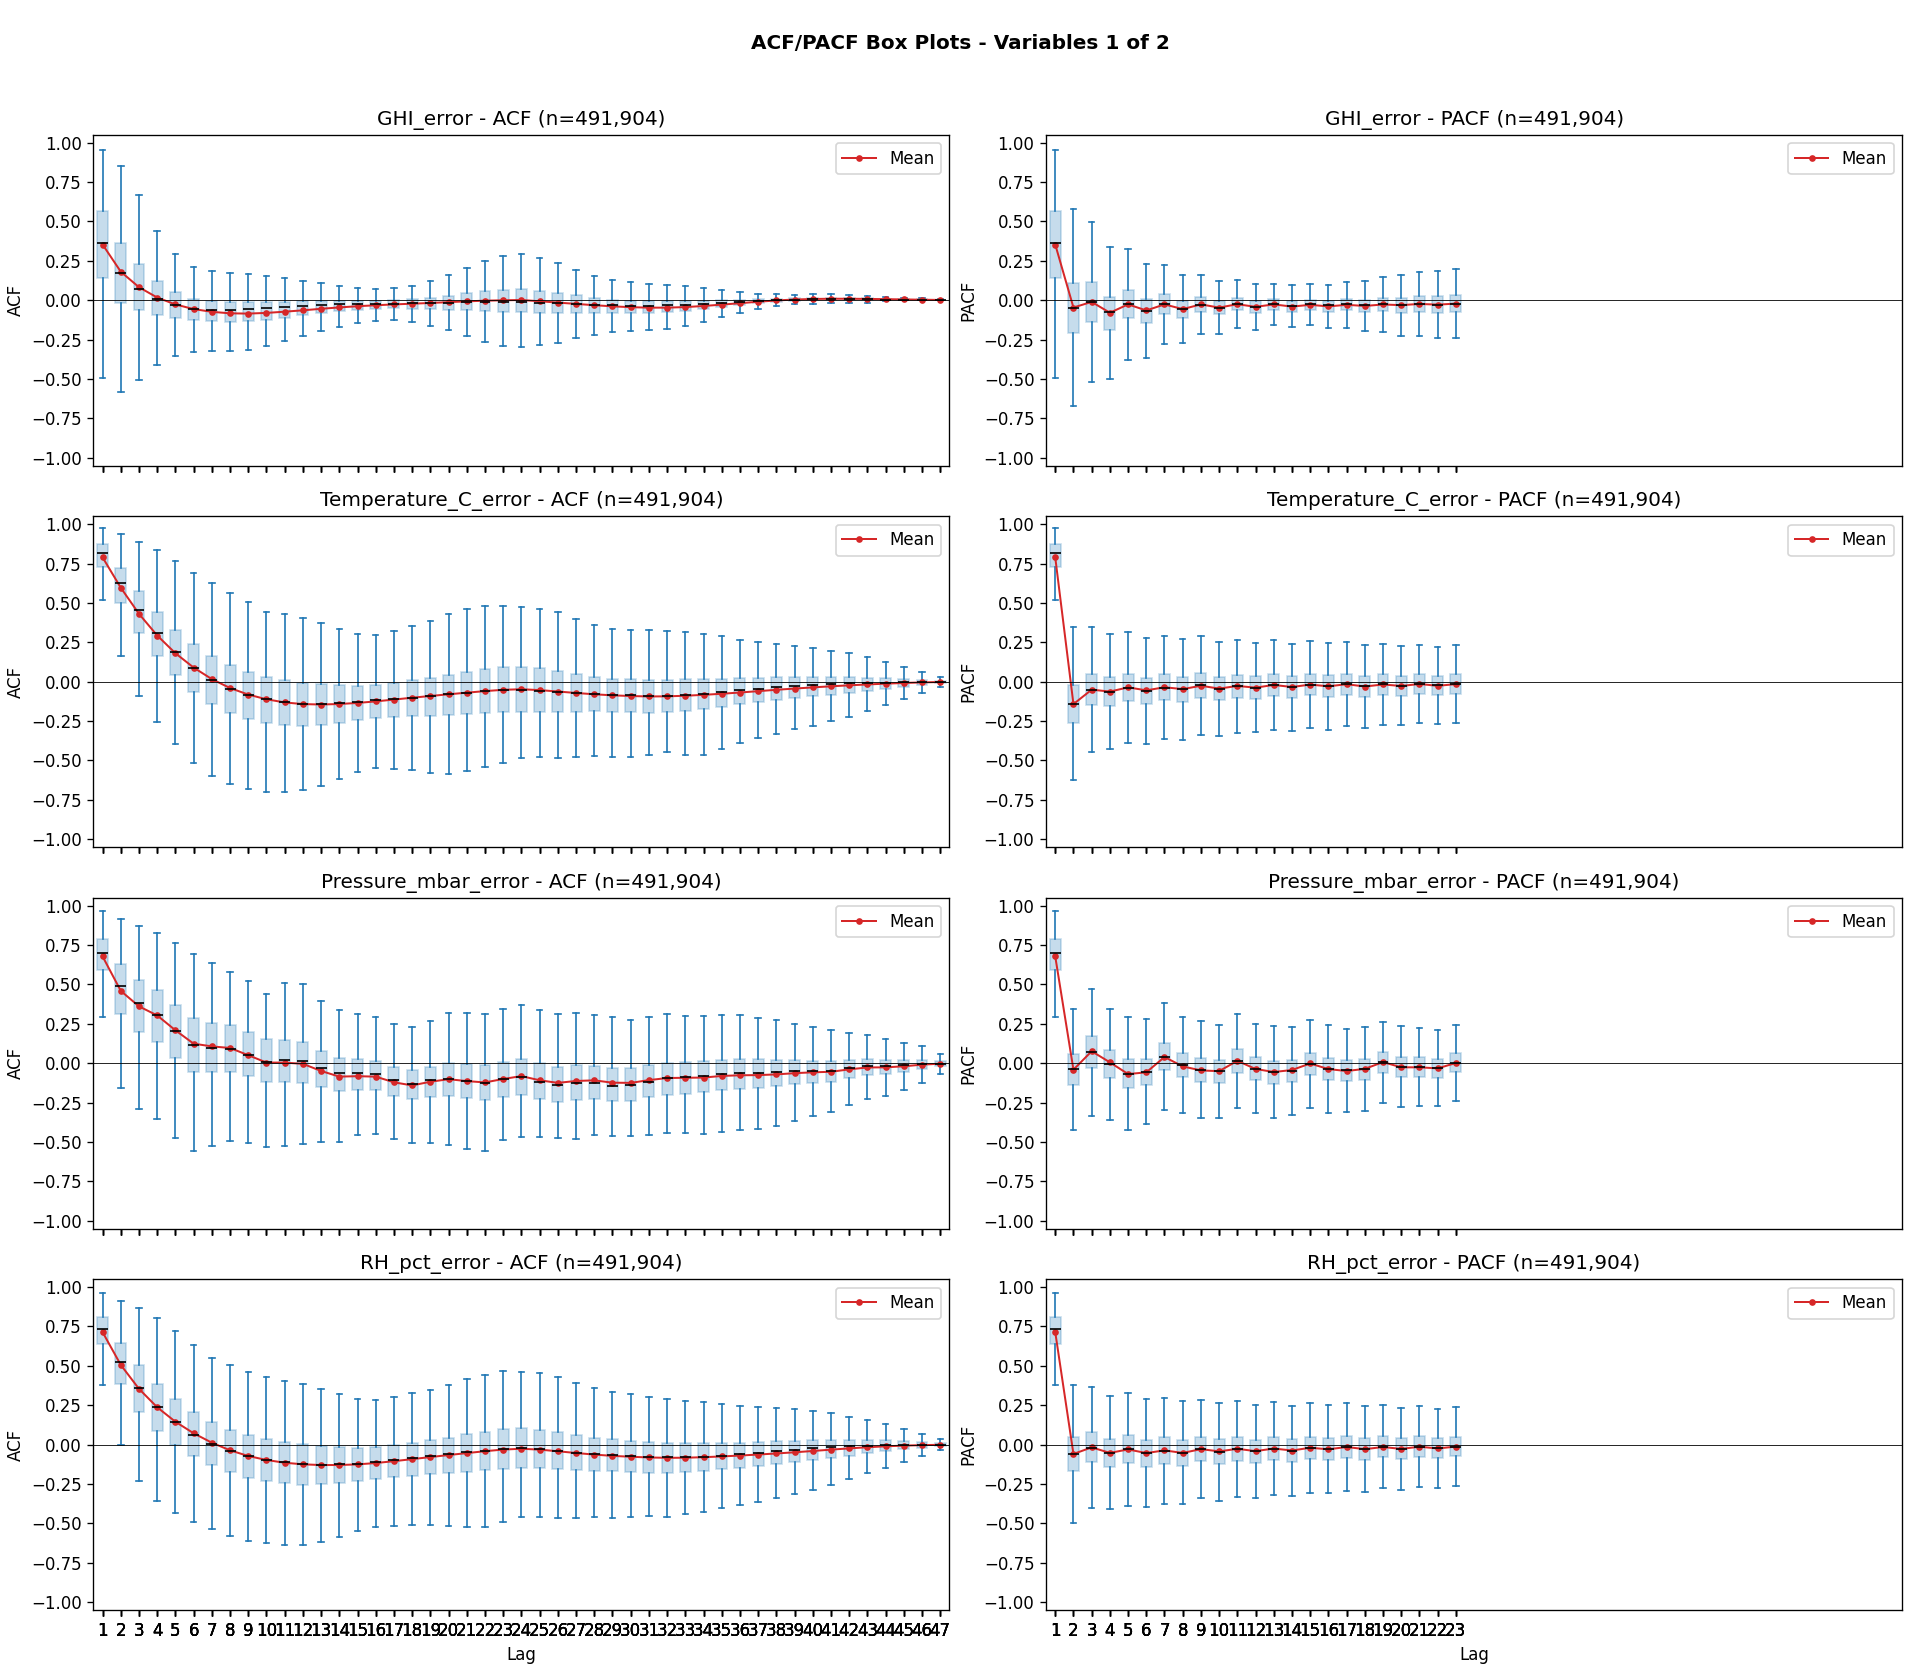
\includegraphics[width=\textwidth]{figures/Q4 & Q5/avg_acf_pacf_variables_01.png}
    \caption{ACF vs. lag on the left and PACF vs. lag on the right for GHI, temperature, pressure, and RH.}
    \label{fig:acf_pacf_vars1}
\end{figure}

\begin{figure}[H]
    \centering
    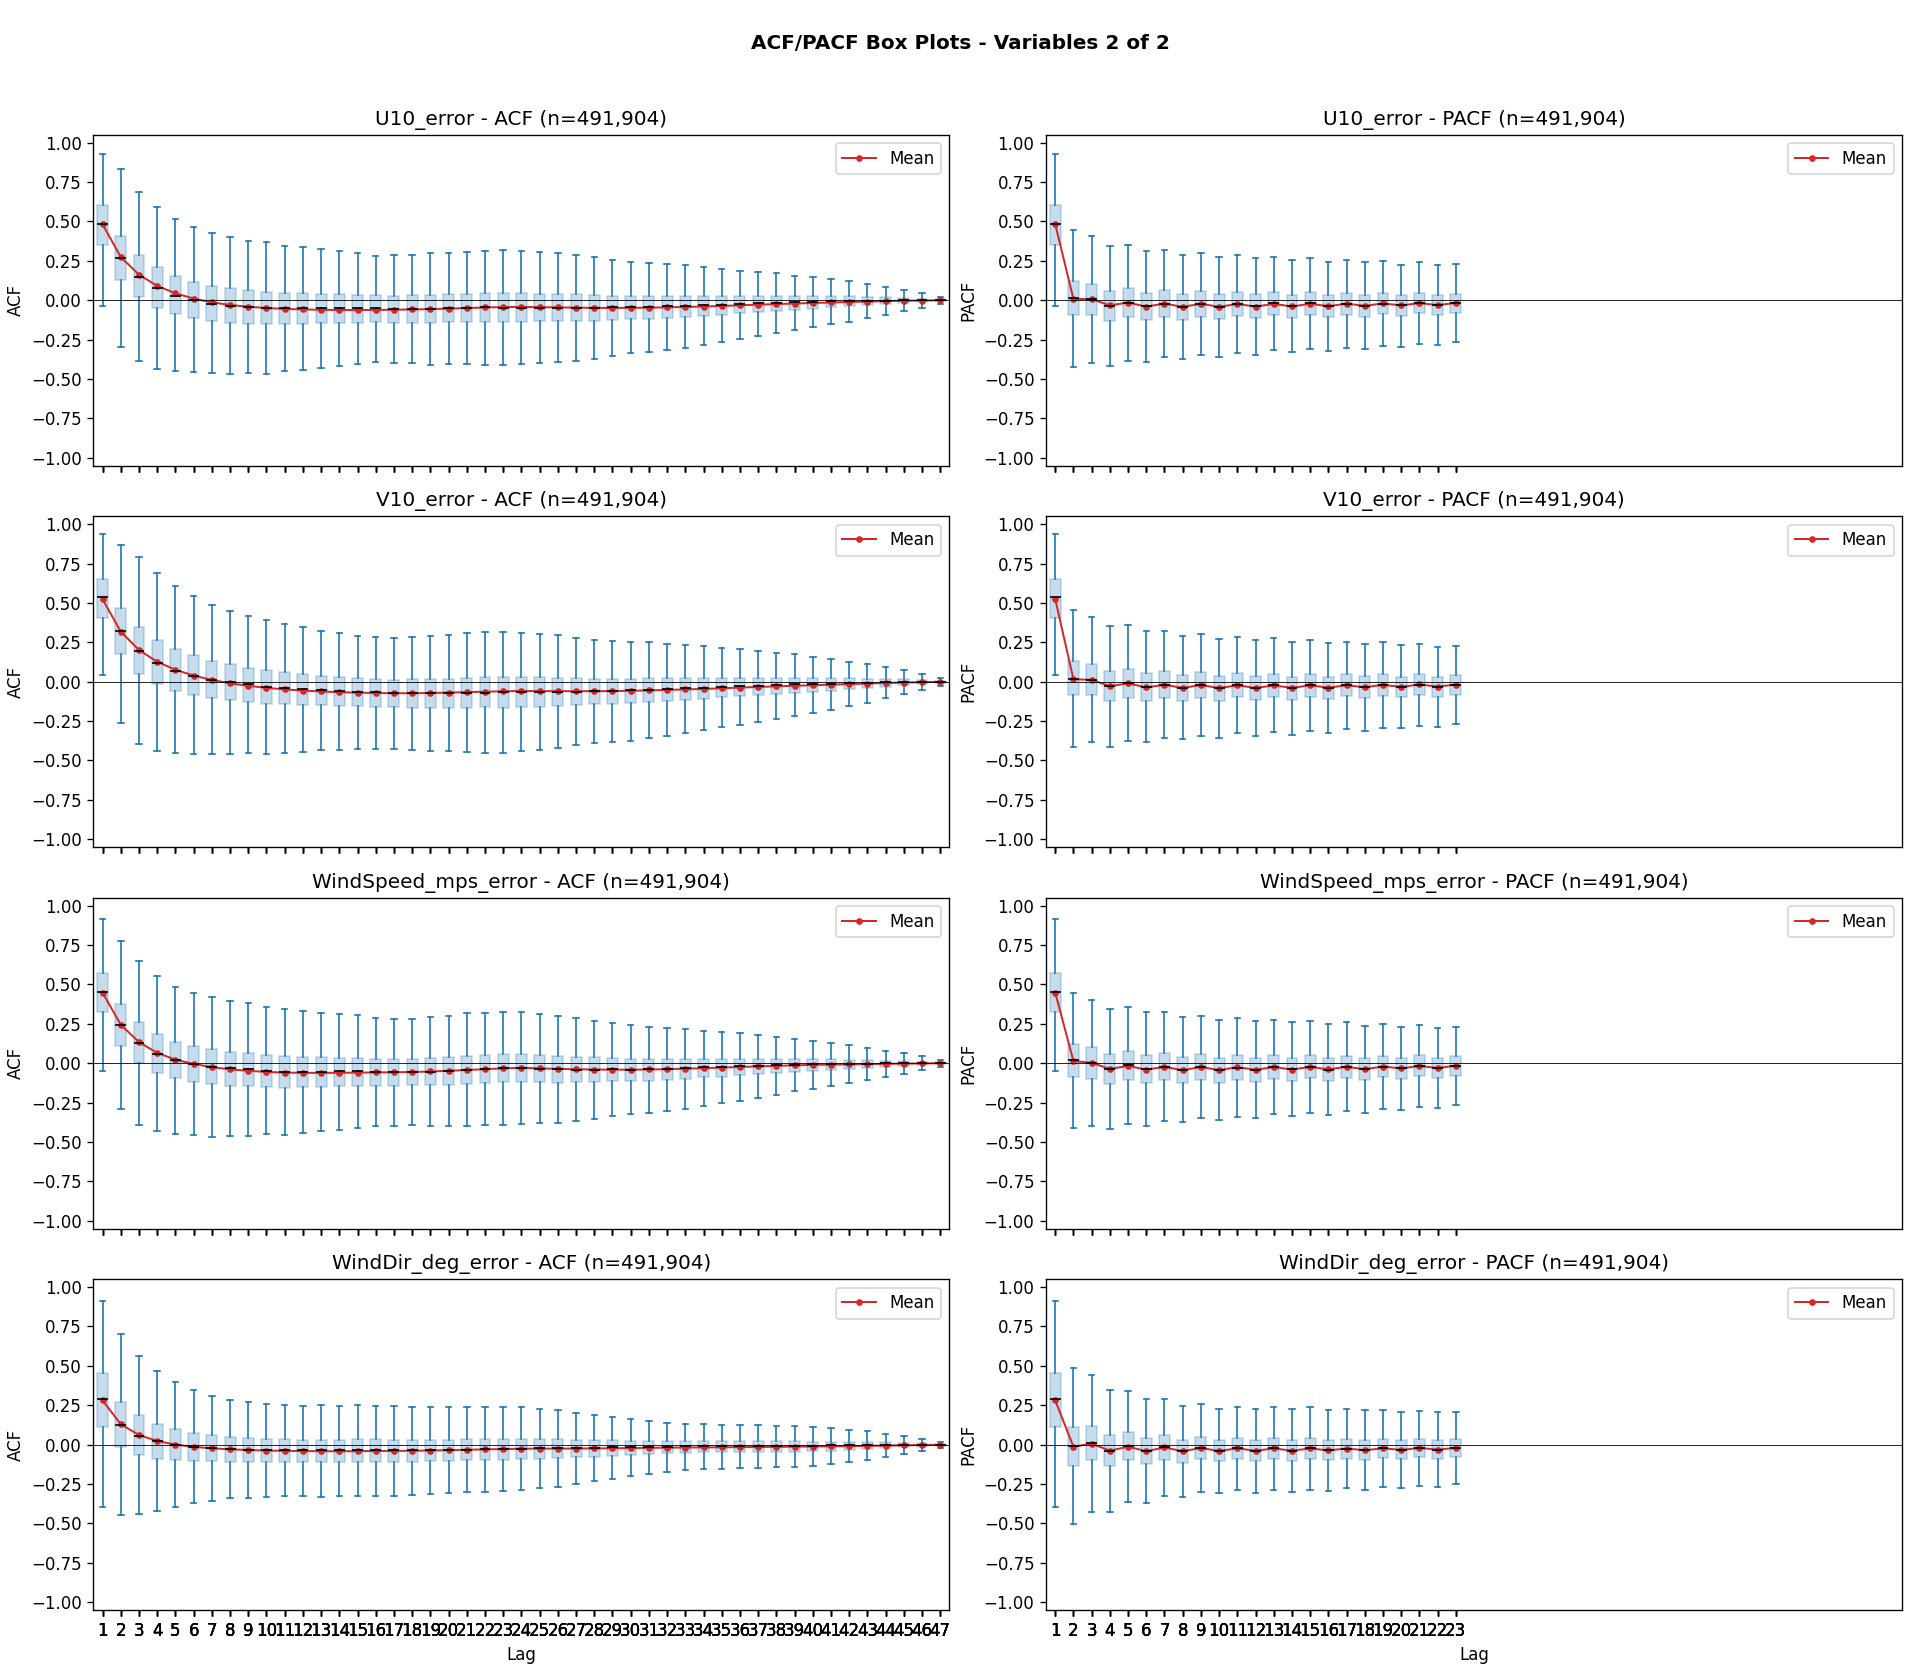
\includegraphics[width=\textwidth]{figures/Q4 & Q5/avg_acf_pacf_variables_02.png}
    \caption{ACF vs. lag on the left and PACF vs. lag on the right for U10, V10, wind speed, and wind direction.}
    \label{fig:acf_pacf_vars2}
\end{figure}

\subsection{Q7 — Stratified Cross-Variable Error Matrices}

% --- DIURNAL EVOLUTION ---
\begin{figure}[H]
  \centering
  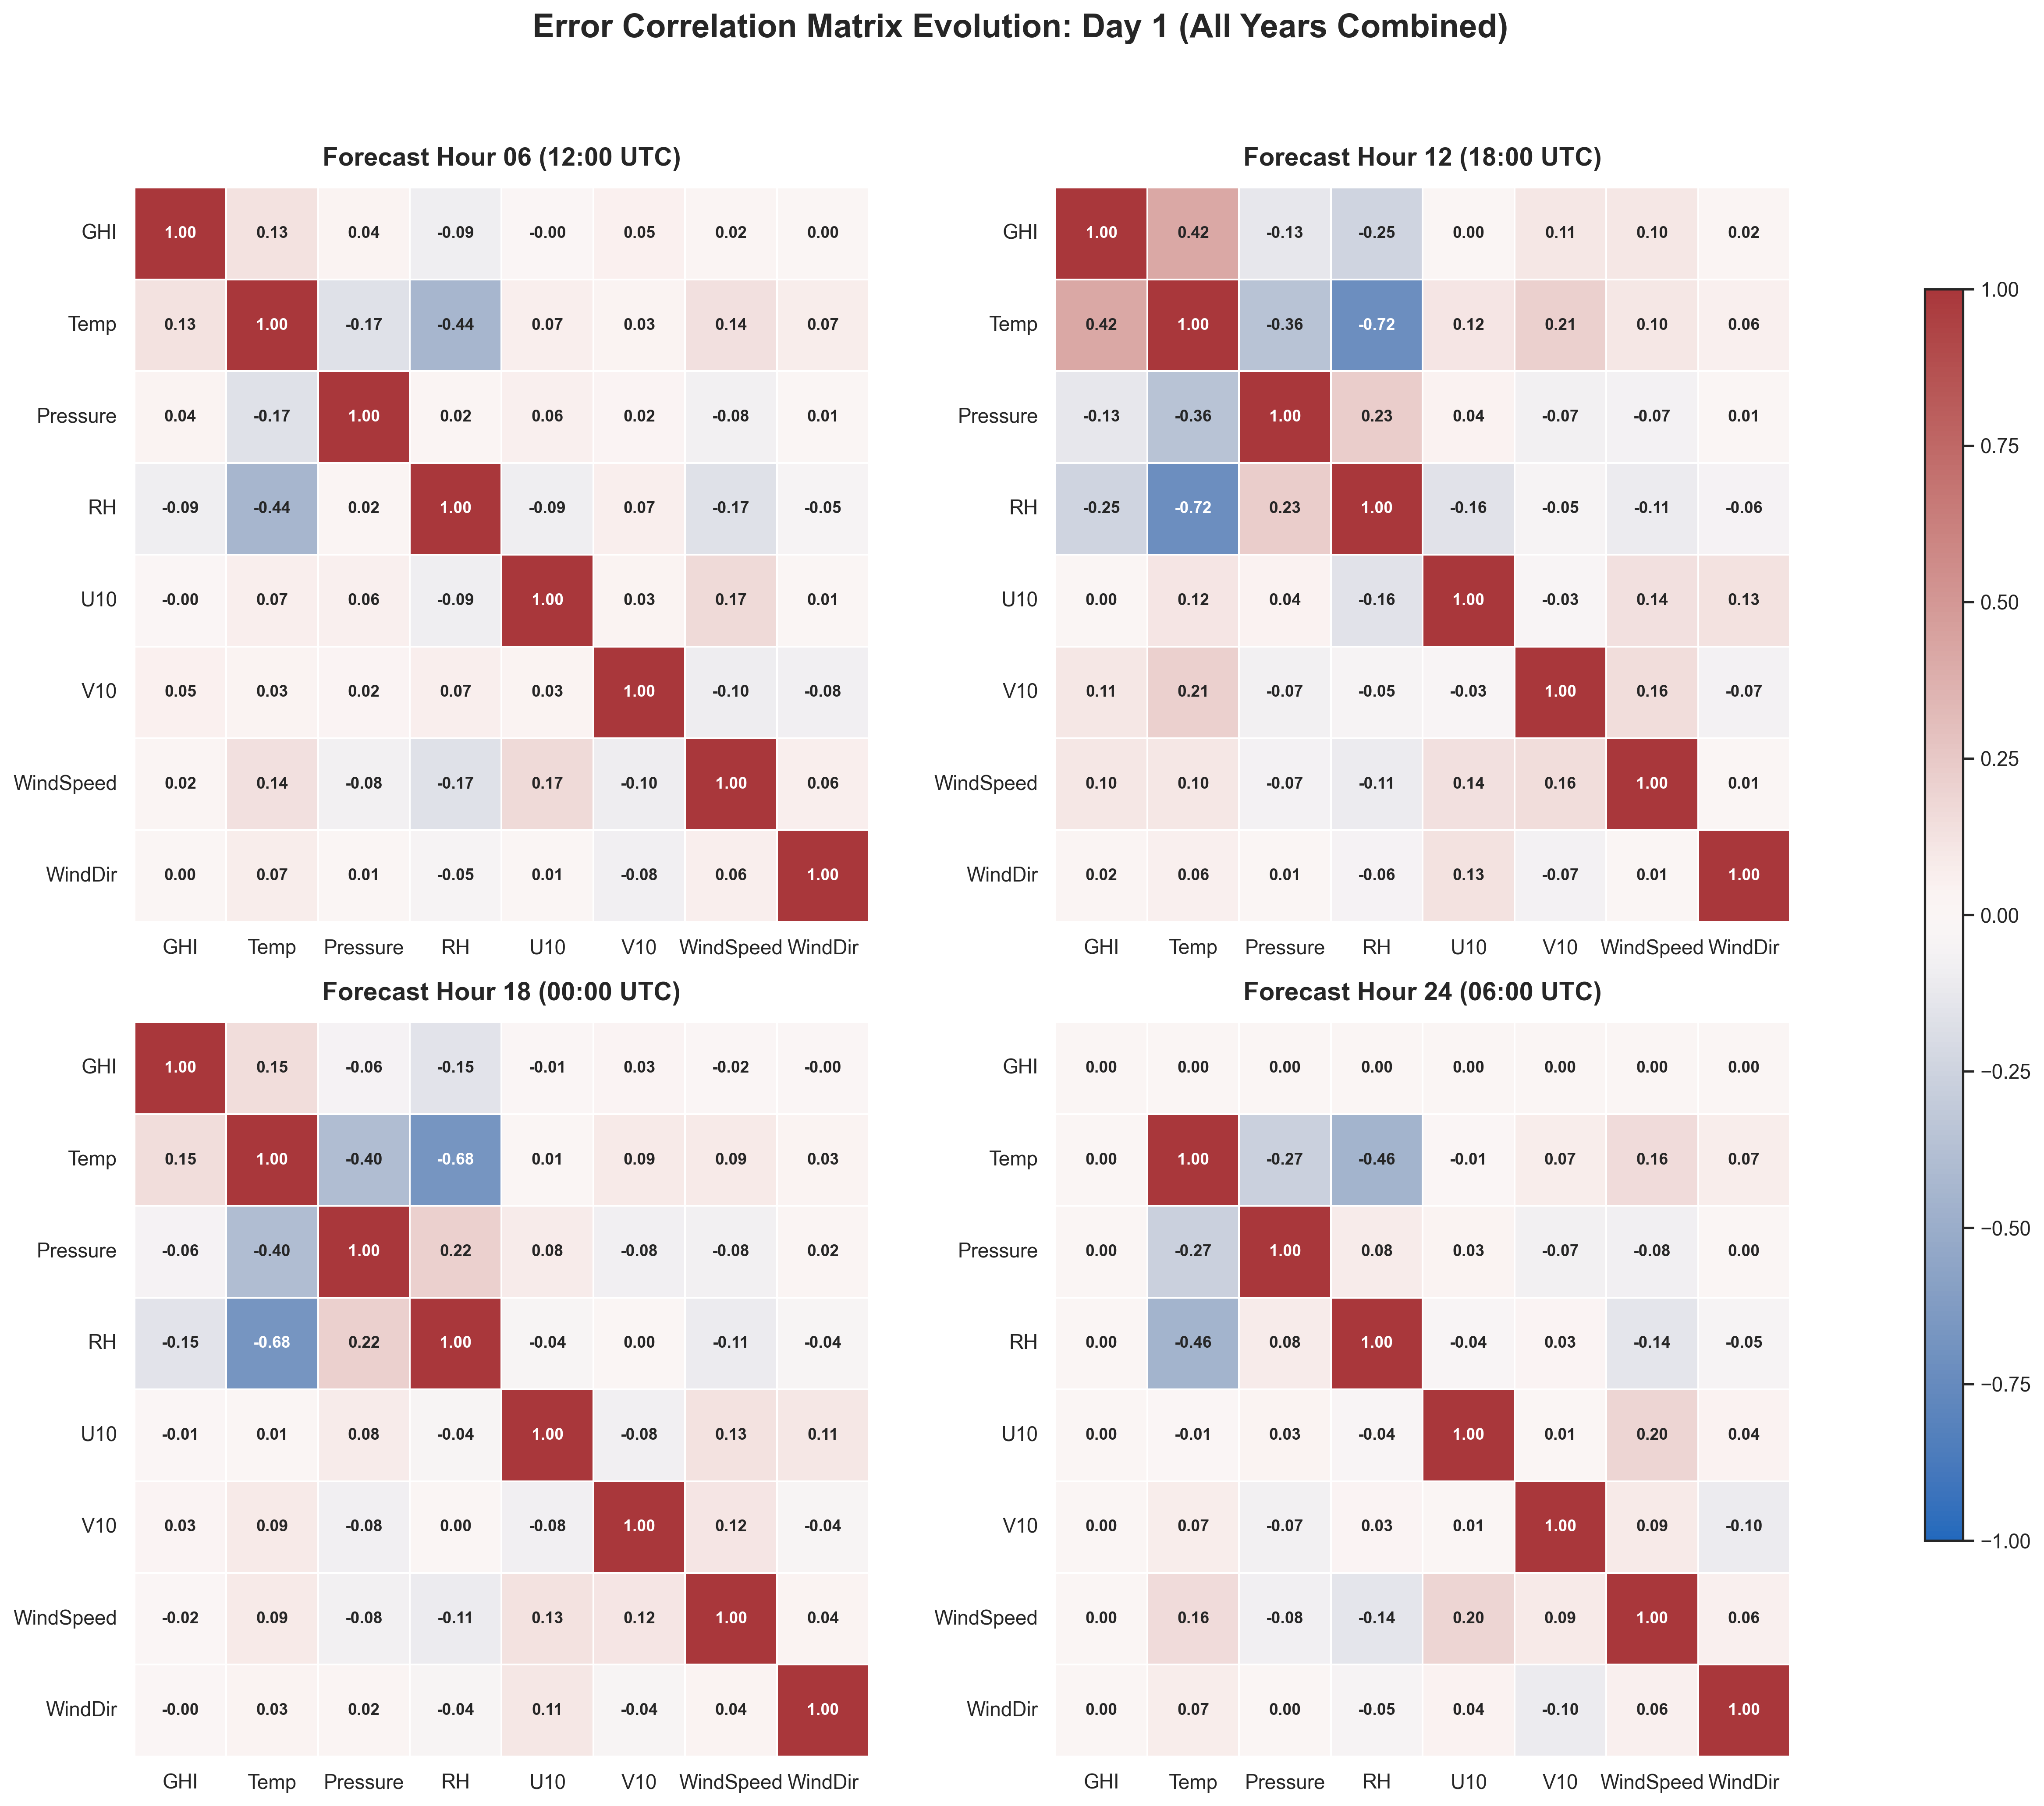
\includegraphics[width=\textwidth]{figures/Q7/TIMEOFDAY/all_variables_corr_day1_horizons.png}
  \caption{Error Correlation Matrix Evolution: Day 1 hourly snapshots across all years combined.}
  \label{fig:app_diurnal_evolution}
\end{figure}

% --- SEASONAL VARIATIONS ---
\begin{figure}[H]
  \centering
  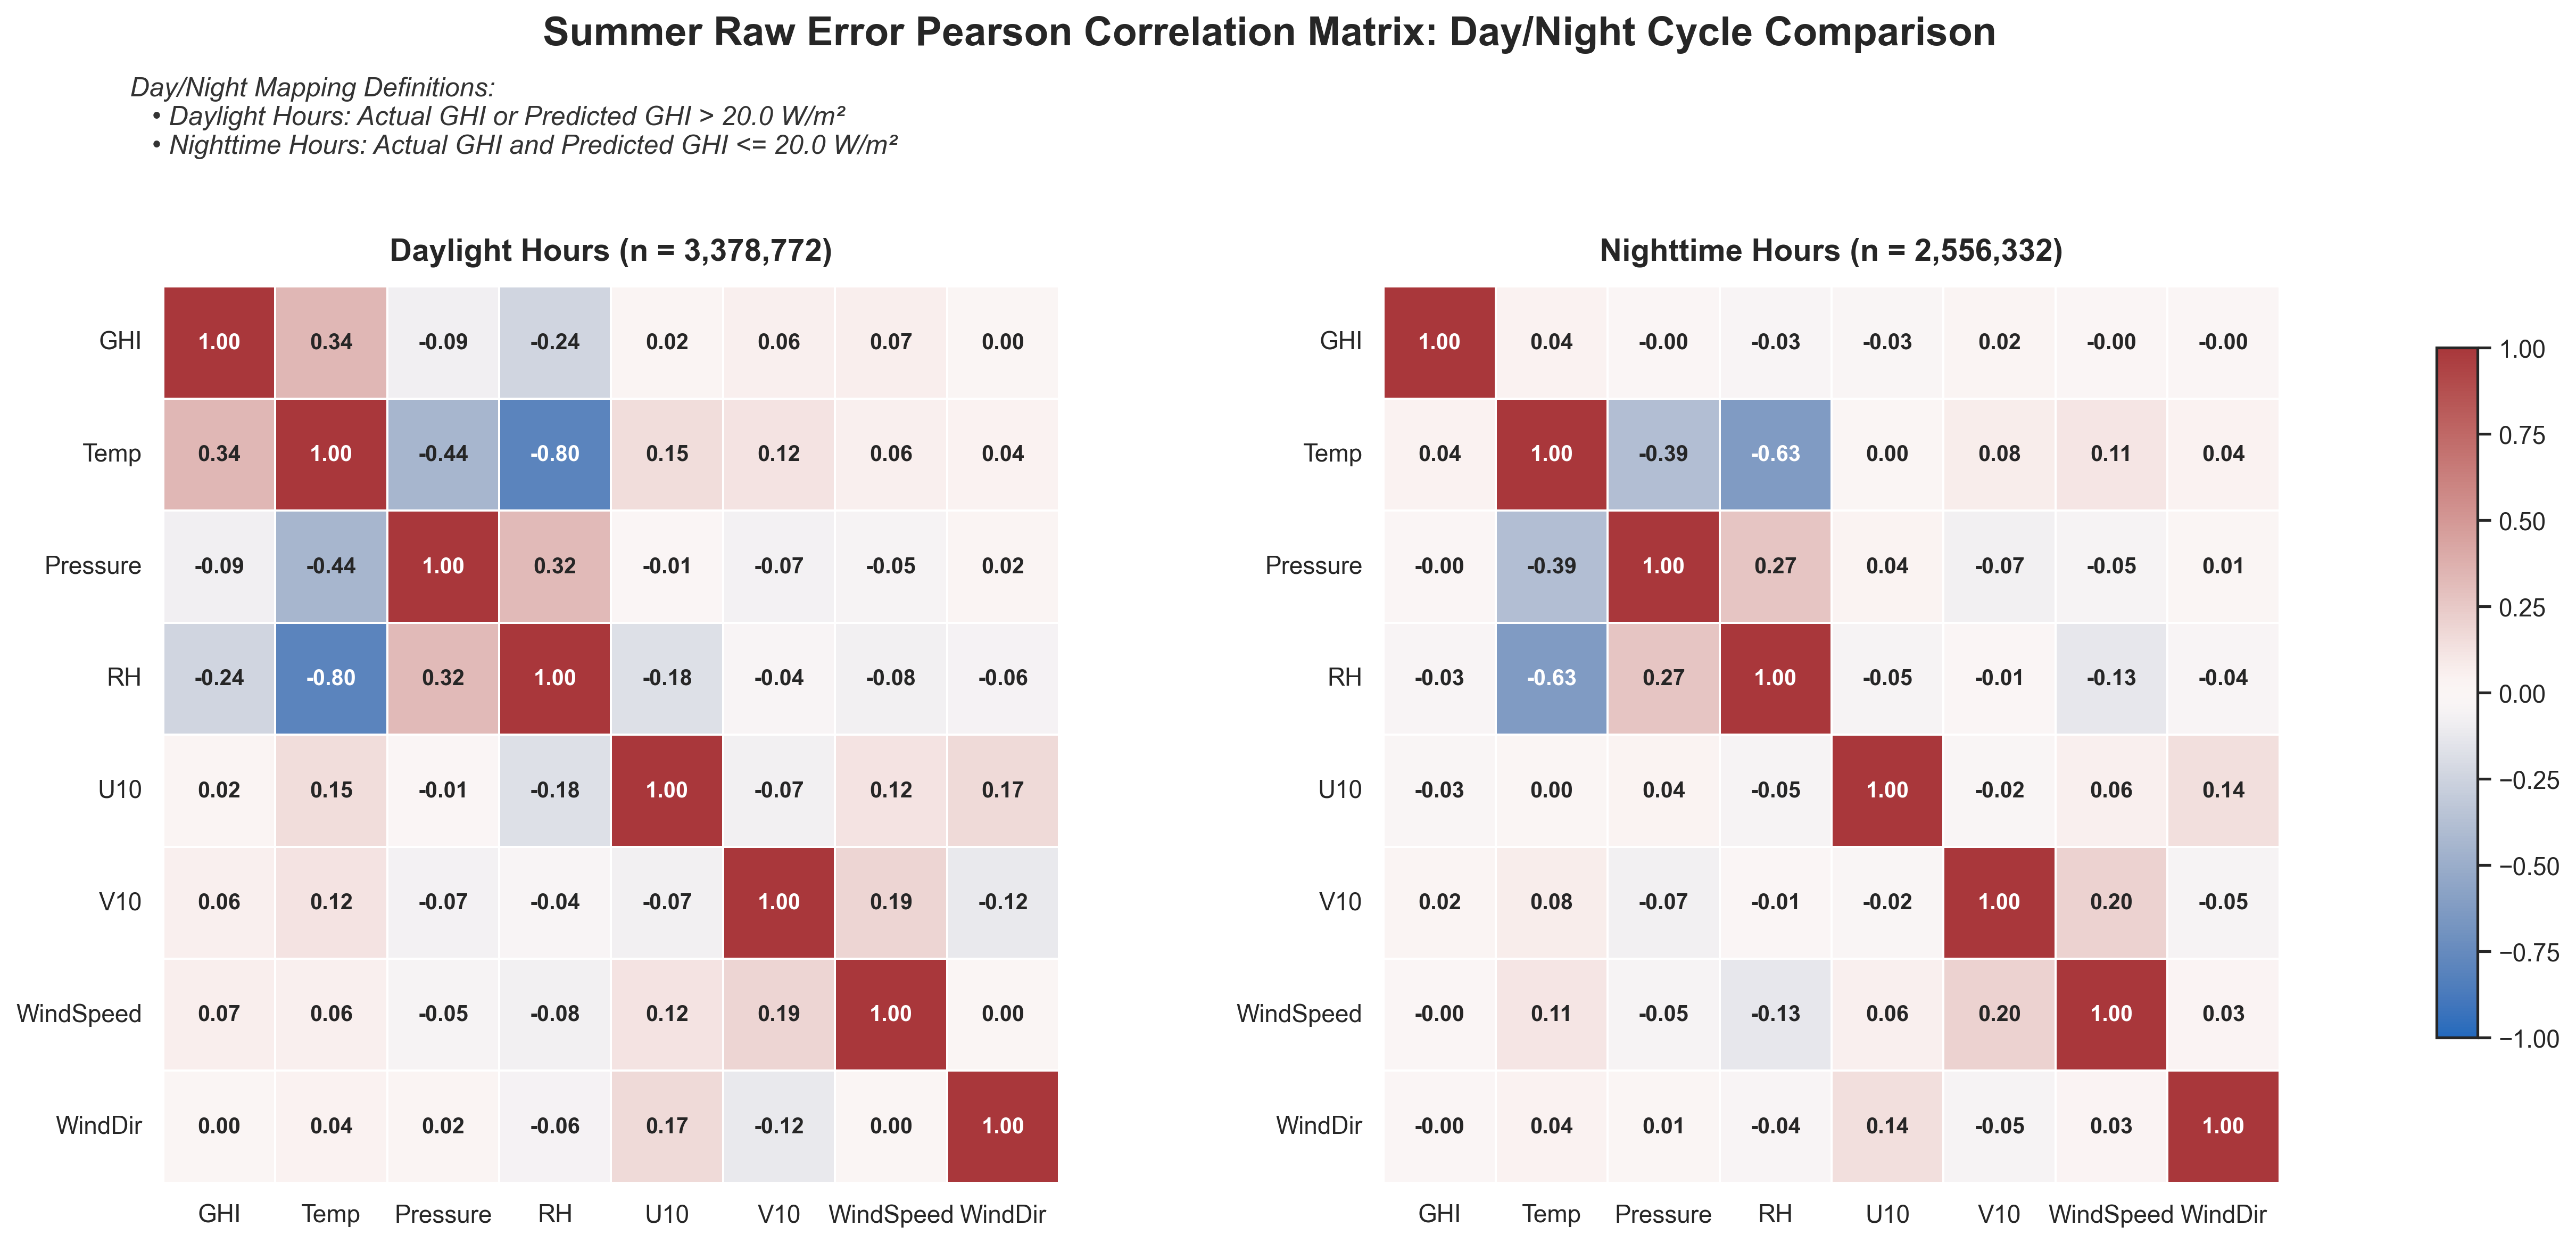
\includegraphics[width=\textwidth]{figures/Q7/SEASONS/correlation_heatmap_summer_diurnal_comparison.png}
  \caption{Summer Raw Error Pearson Correlation Matrix: Daylight Hours ($n = 3,378,772$, left) versus Nighttime Hours ($n = 2,556,332$, right) comparison.}
  \label{fig:app_summer_day_night}
\end{figure}

\begin{figure}[H]
  \centering
  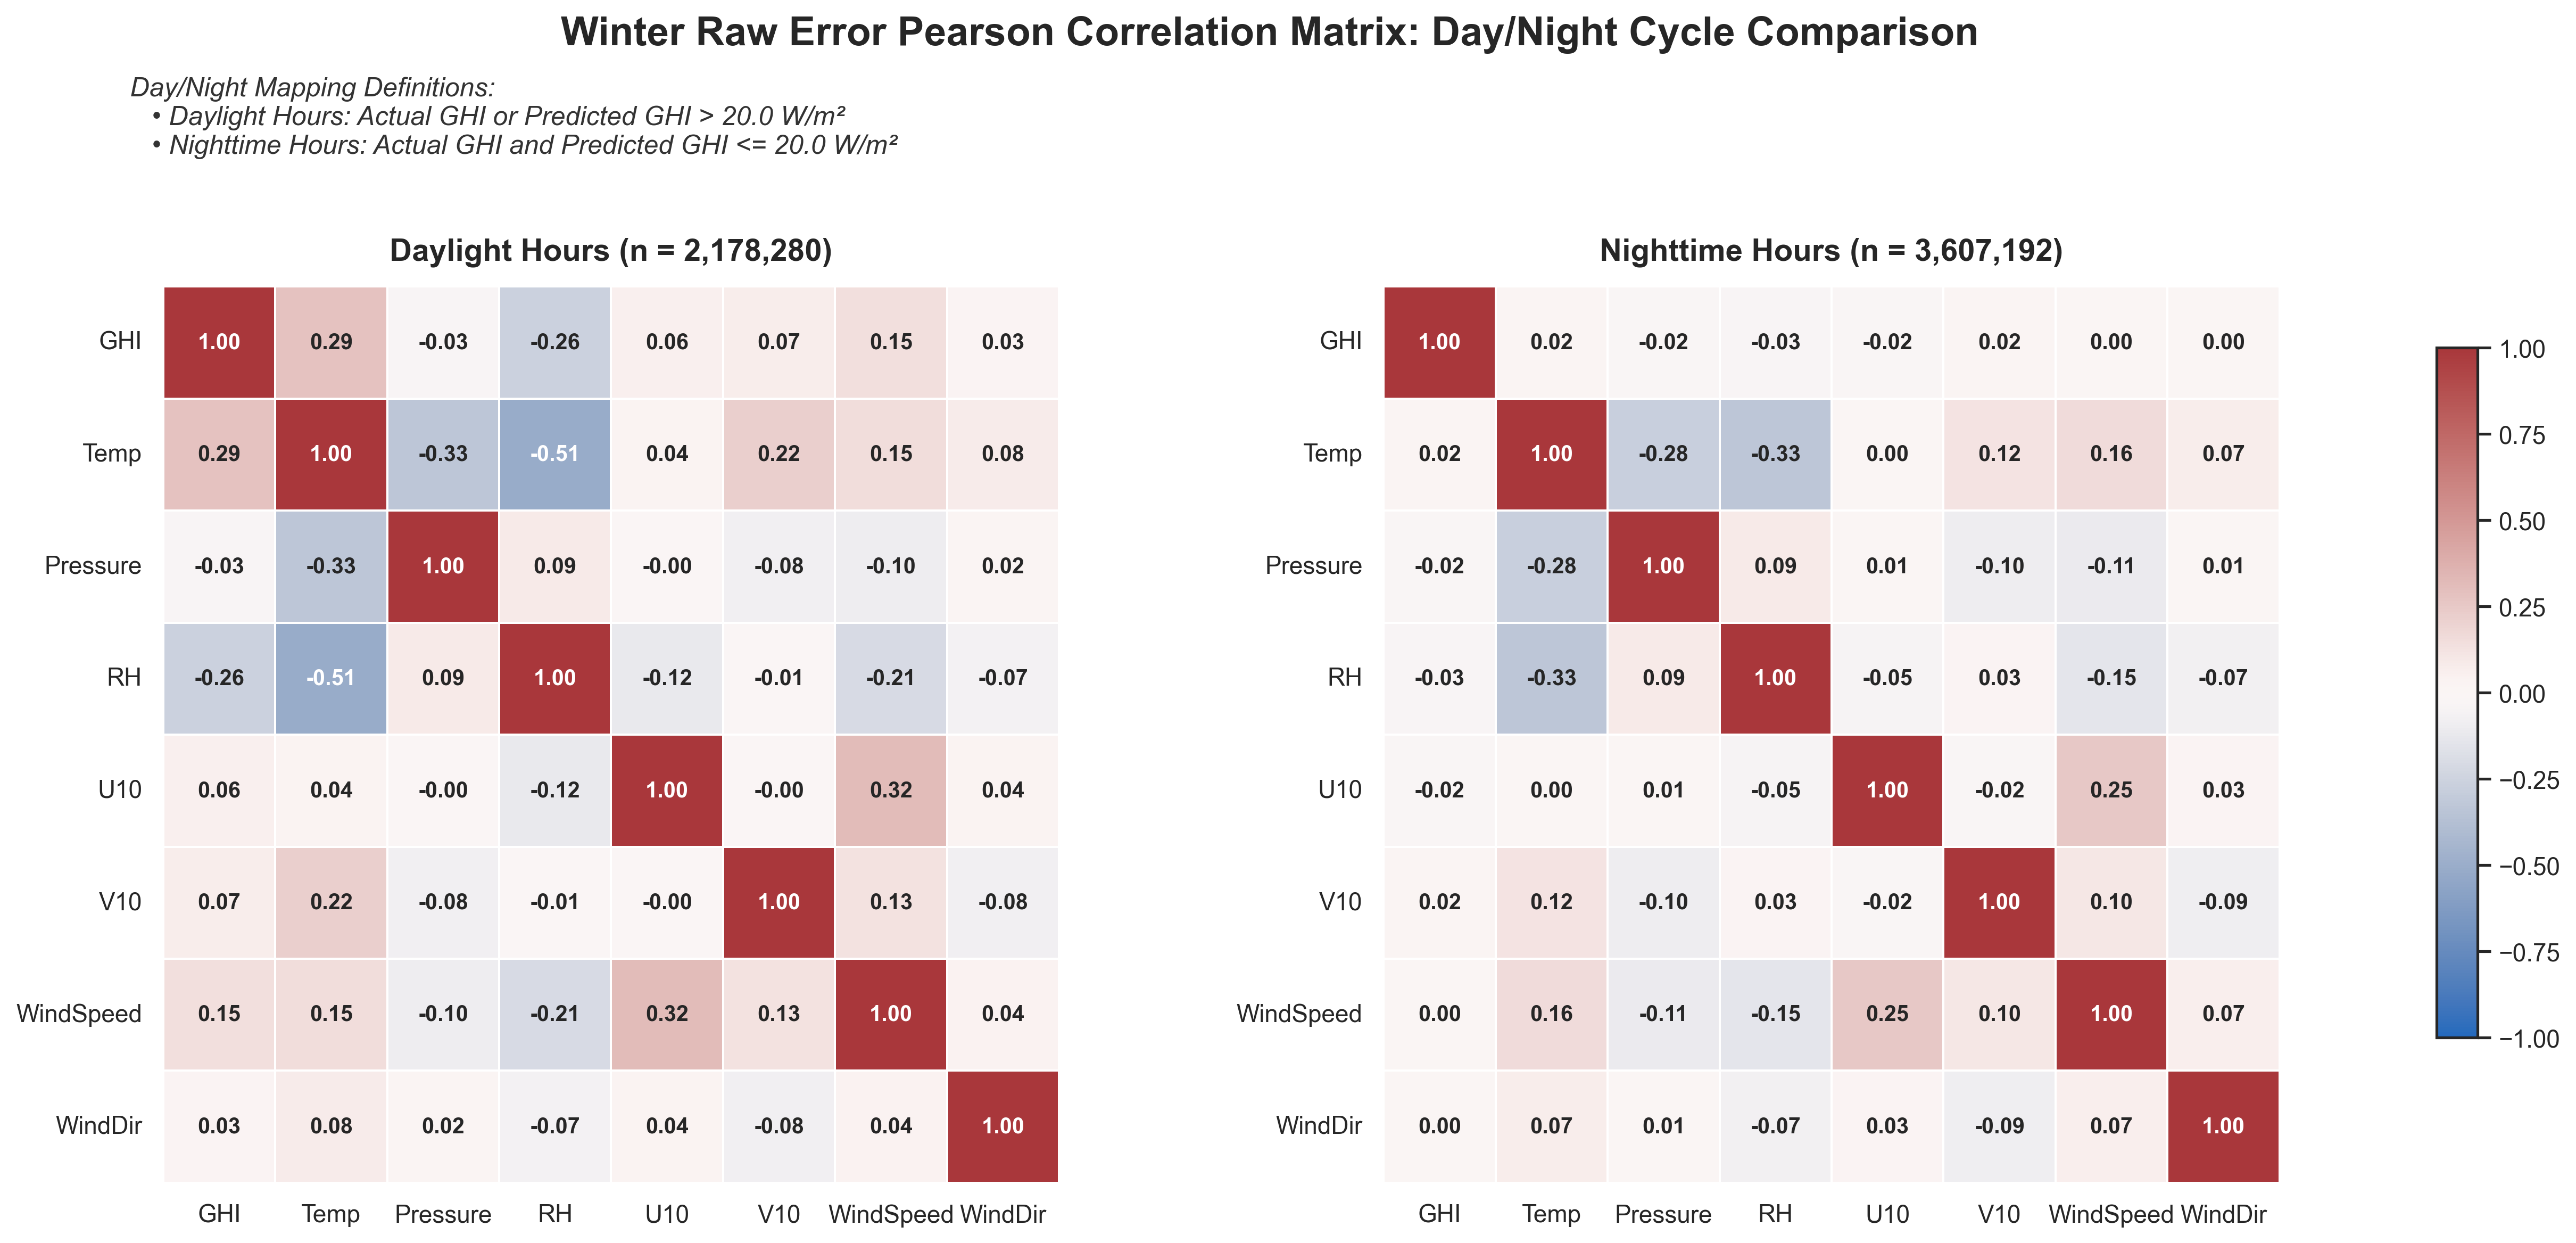
\includegraphics[width=\textwidth]{figures/Q7/SEASONS/correlation_heatmap_winter_diurnal_comparison.png}
  \caption{Winter Raw Error Pearson Correlation Matrix: Daylight vs. Nighttime comparison.}
  \label{fig:app_winter_day_night}
\end{figure}

\begin{figure}[H]
  \centering
  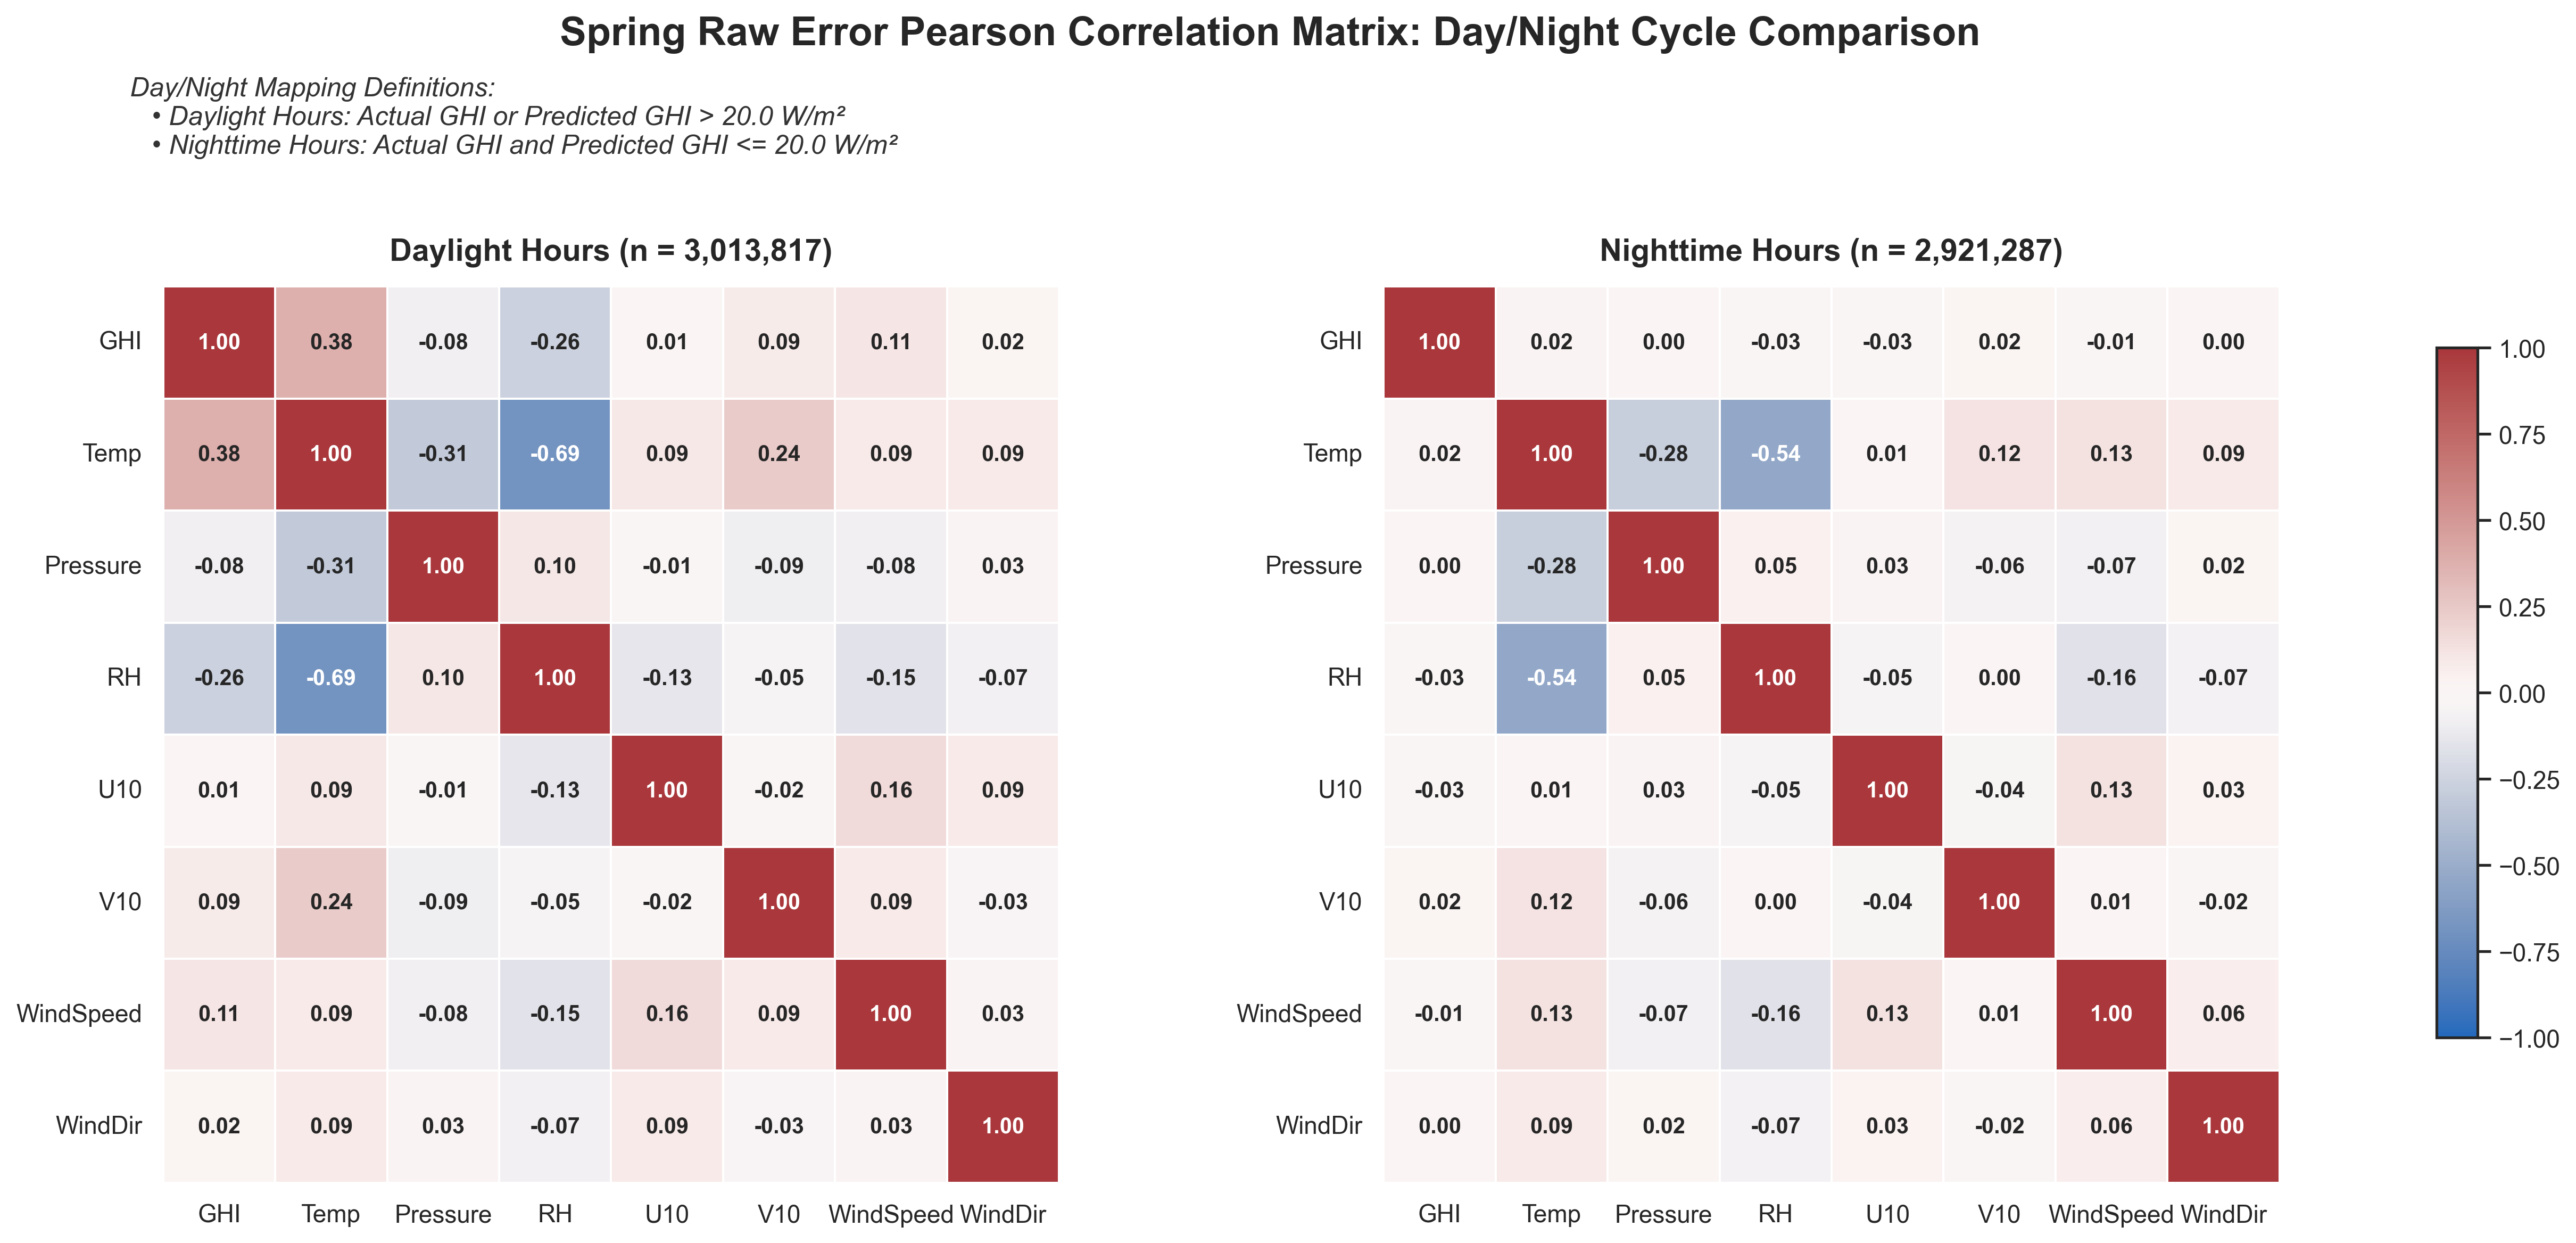
\includegraphics[width=\textwidth]{figures/Q7/SEASONS/correlation_heatmap_spring_diurnal_comparison.png}
  \caption{Spring Raw Error Pearson Correlation Matrix: Daylight Hours ($n = 3,013,817$, left) versus Nighttime Hours ($n = 2,921,287$, right) comparison.}
  \label{fig:app_spring_day_night}
\end{figure}

\begin{figure}[H]
  \centering
  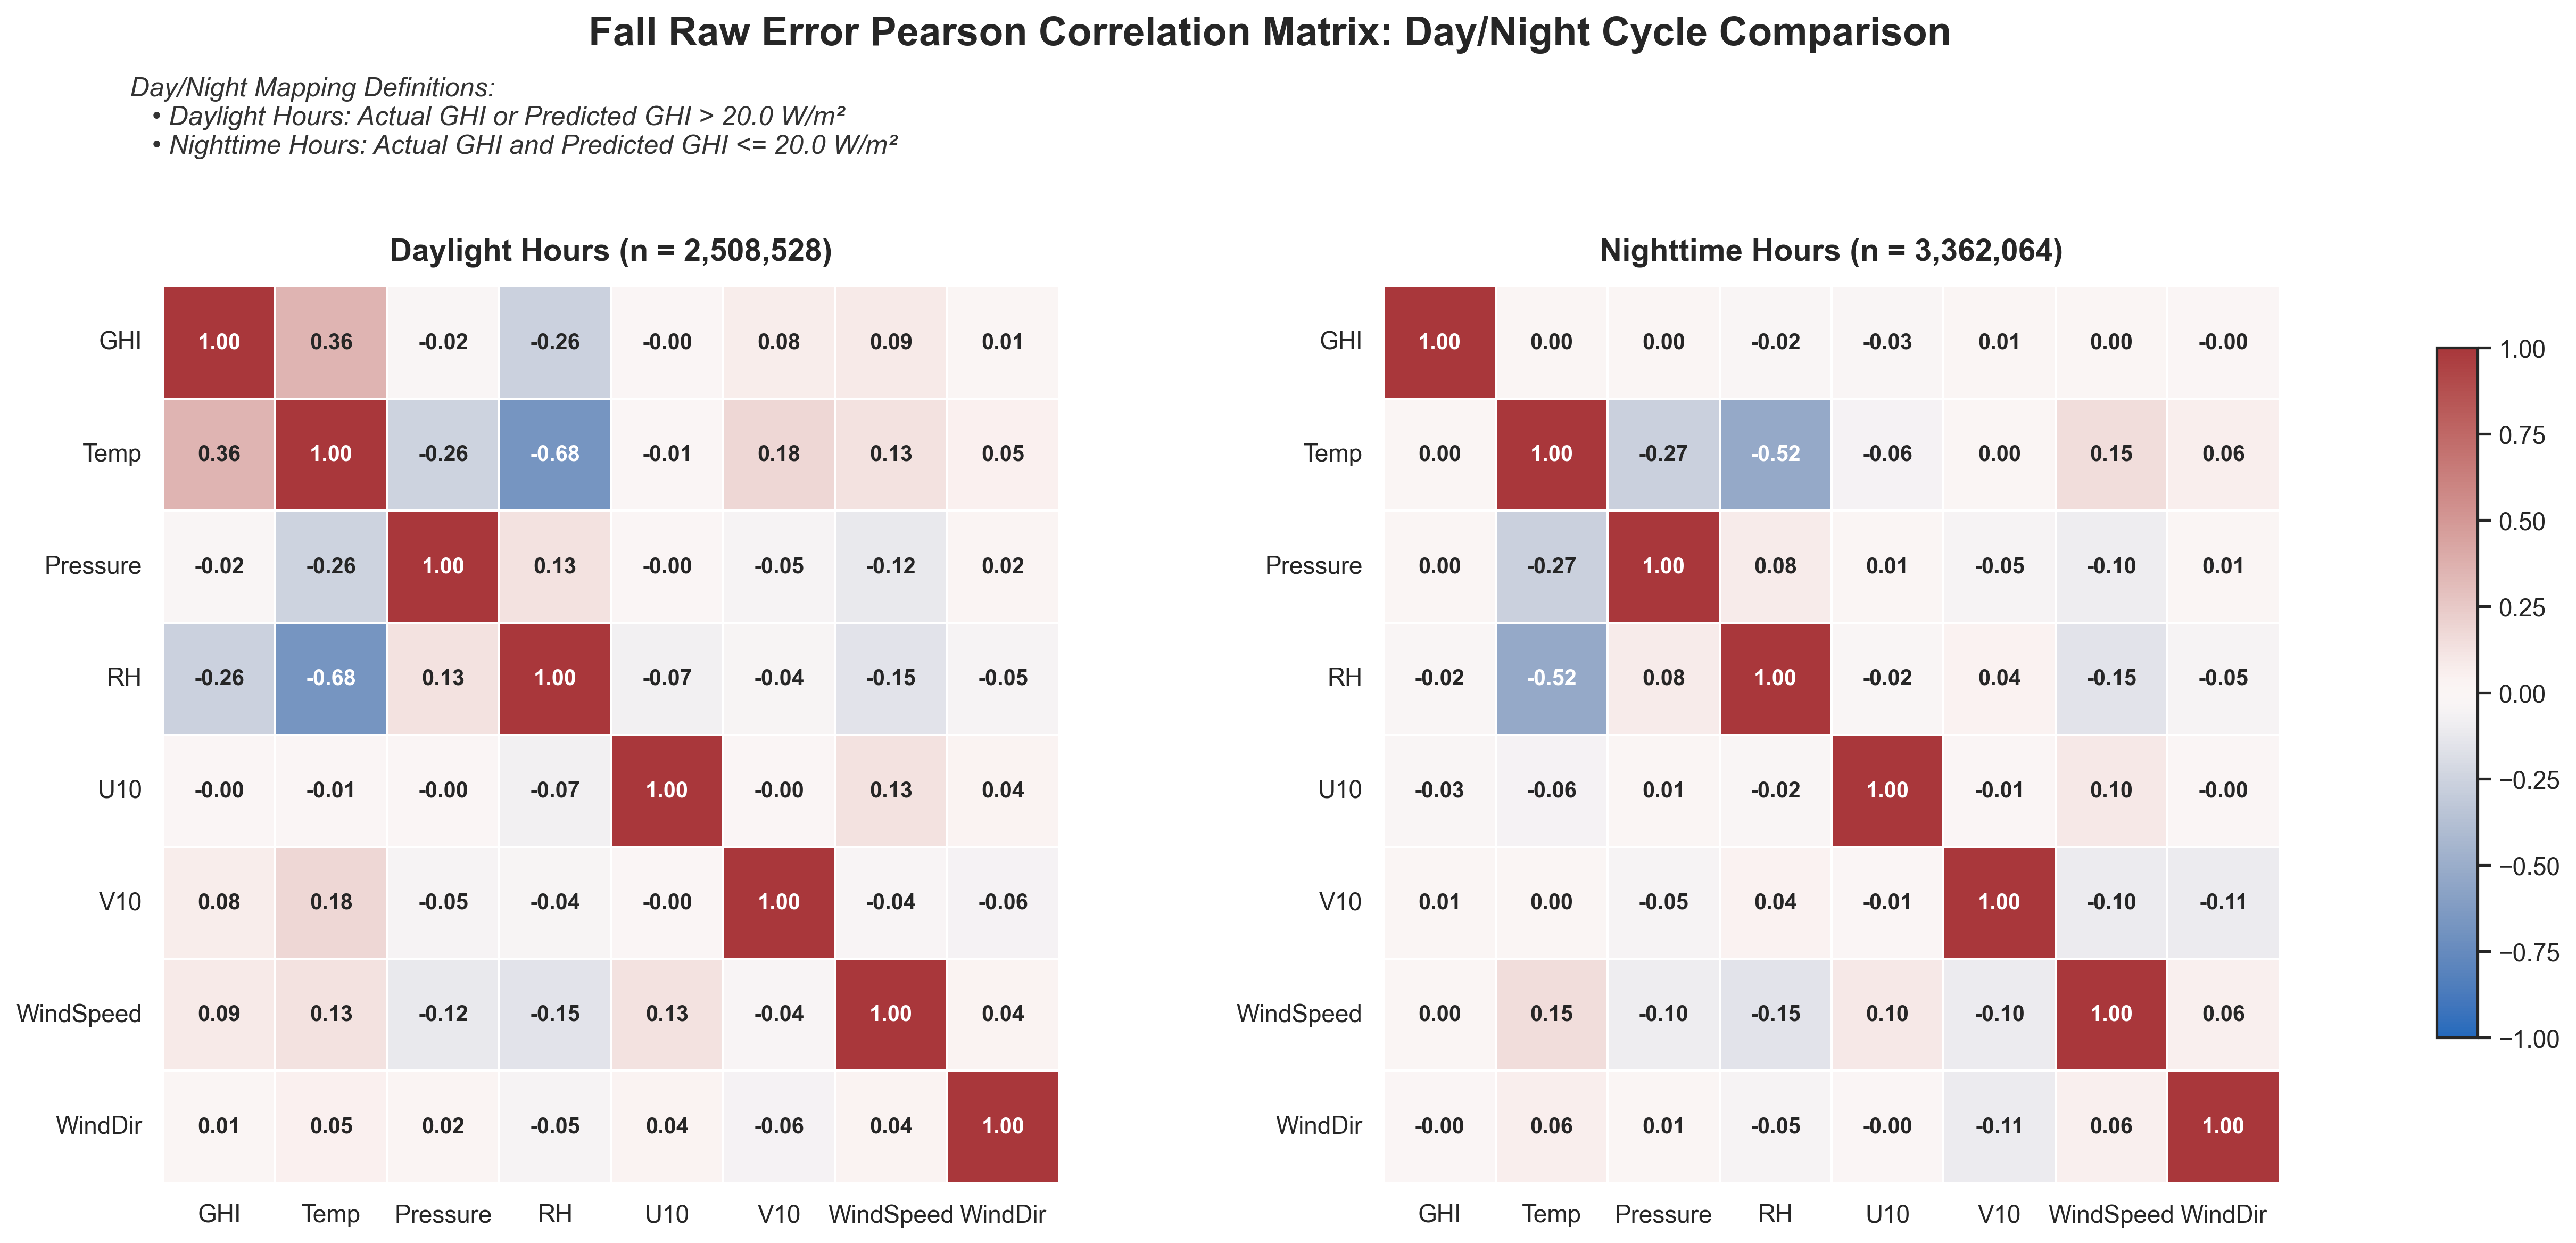
\includegraphics[width=\textwidth]{figures/Q7/SEASONS/correlation_heatmap_fall_diurnal_comparison.png}
  \caption{Fall Raw Error Pearson Correlation Matrix: Daylight Hours ($n = 2,508,528$, left) versus Nighttime Hours ($n = 3,362,064$, right) comparison.}
  \label{fig:app_fall_day_night}
\end{figure}

% --- INTERANNUAL VARIATIONS ---
\begin{figure}[H]
  \centering
  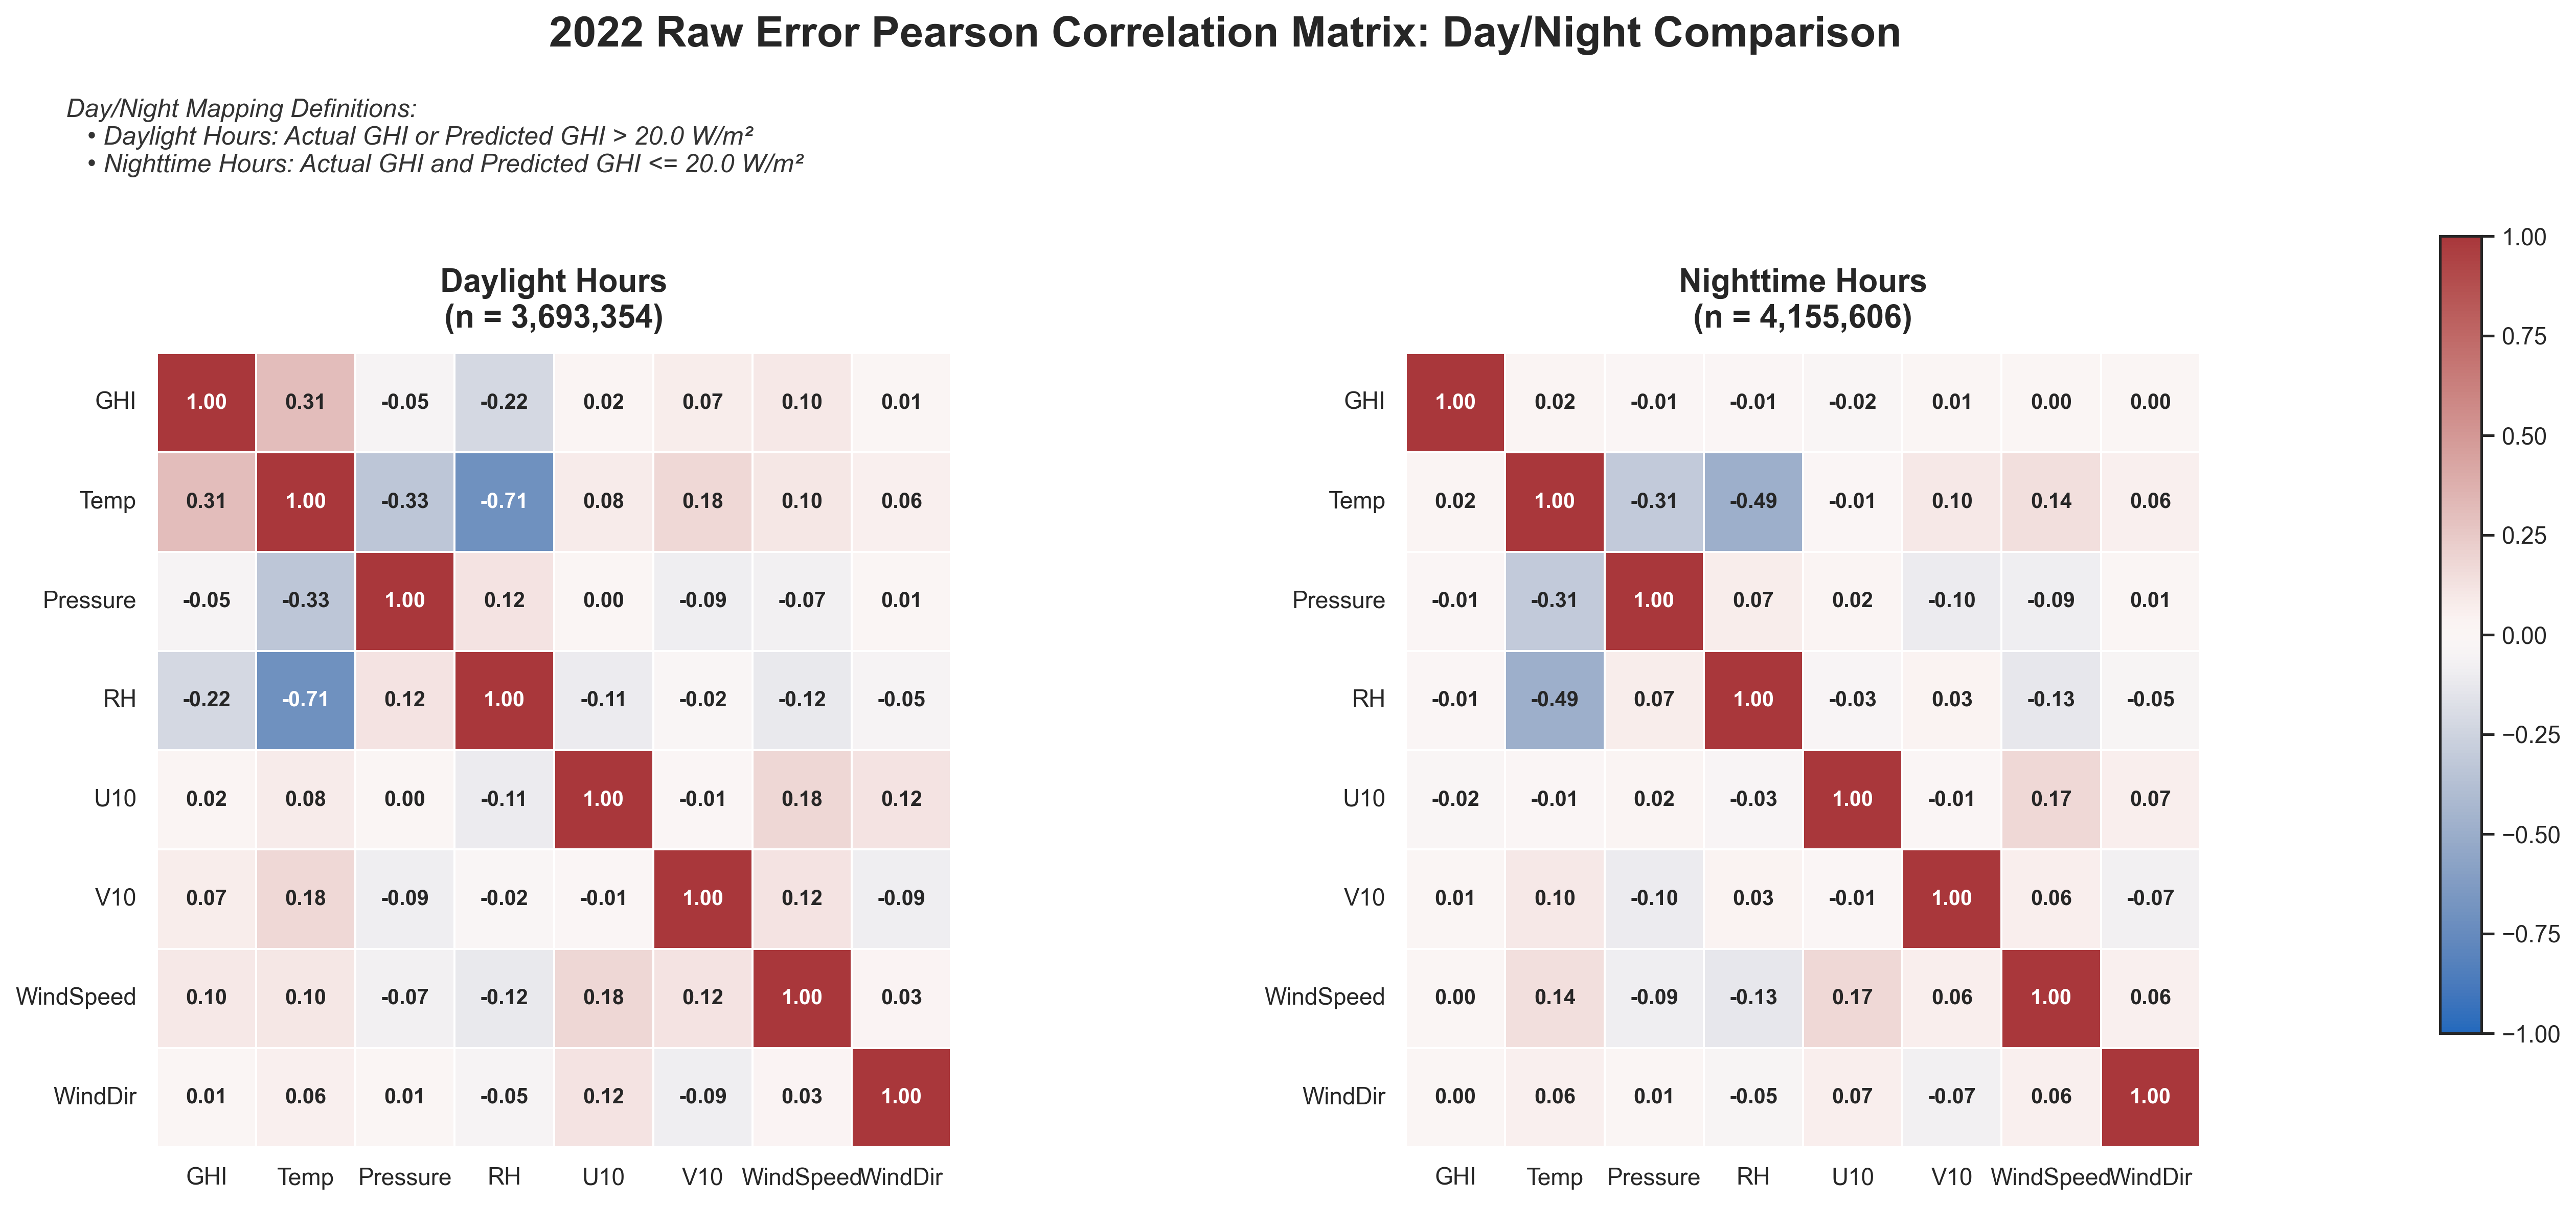
\includegraphics[width=\textwidth]{figures/Q7/YEARS/annual_corr_diurnal_split_2022.png}
  \caption{2022 Raw Error Pearson Correlation Matrix: Daylight Hours ($n = 3,693,554$, left) versus Nighttime Hours ($n = 4,155,606$, right) comparison.}
  \label{fig:app_corr_2022}
\end{figure}

\begin{figure}[H]
  \centering
  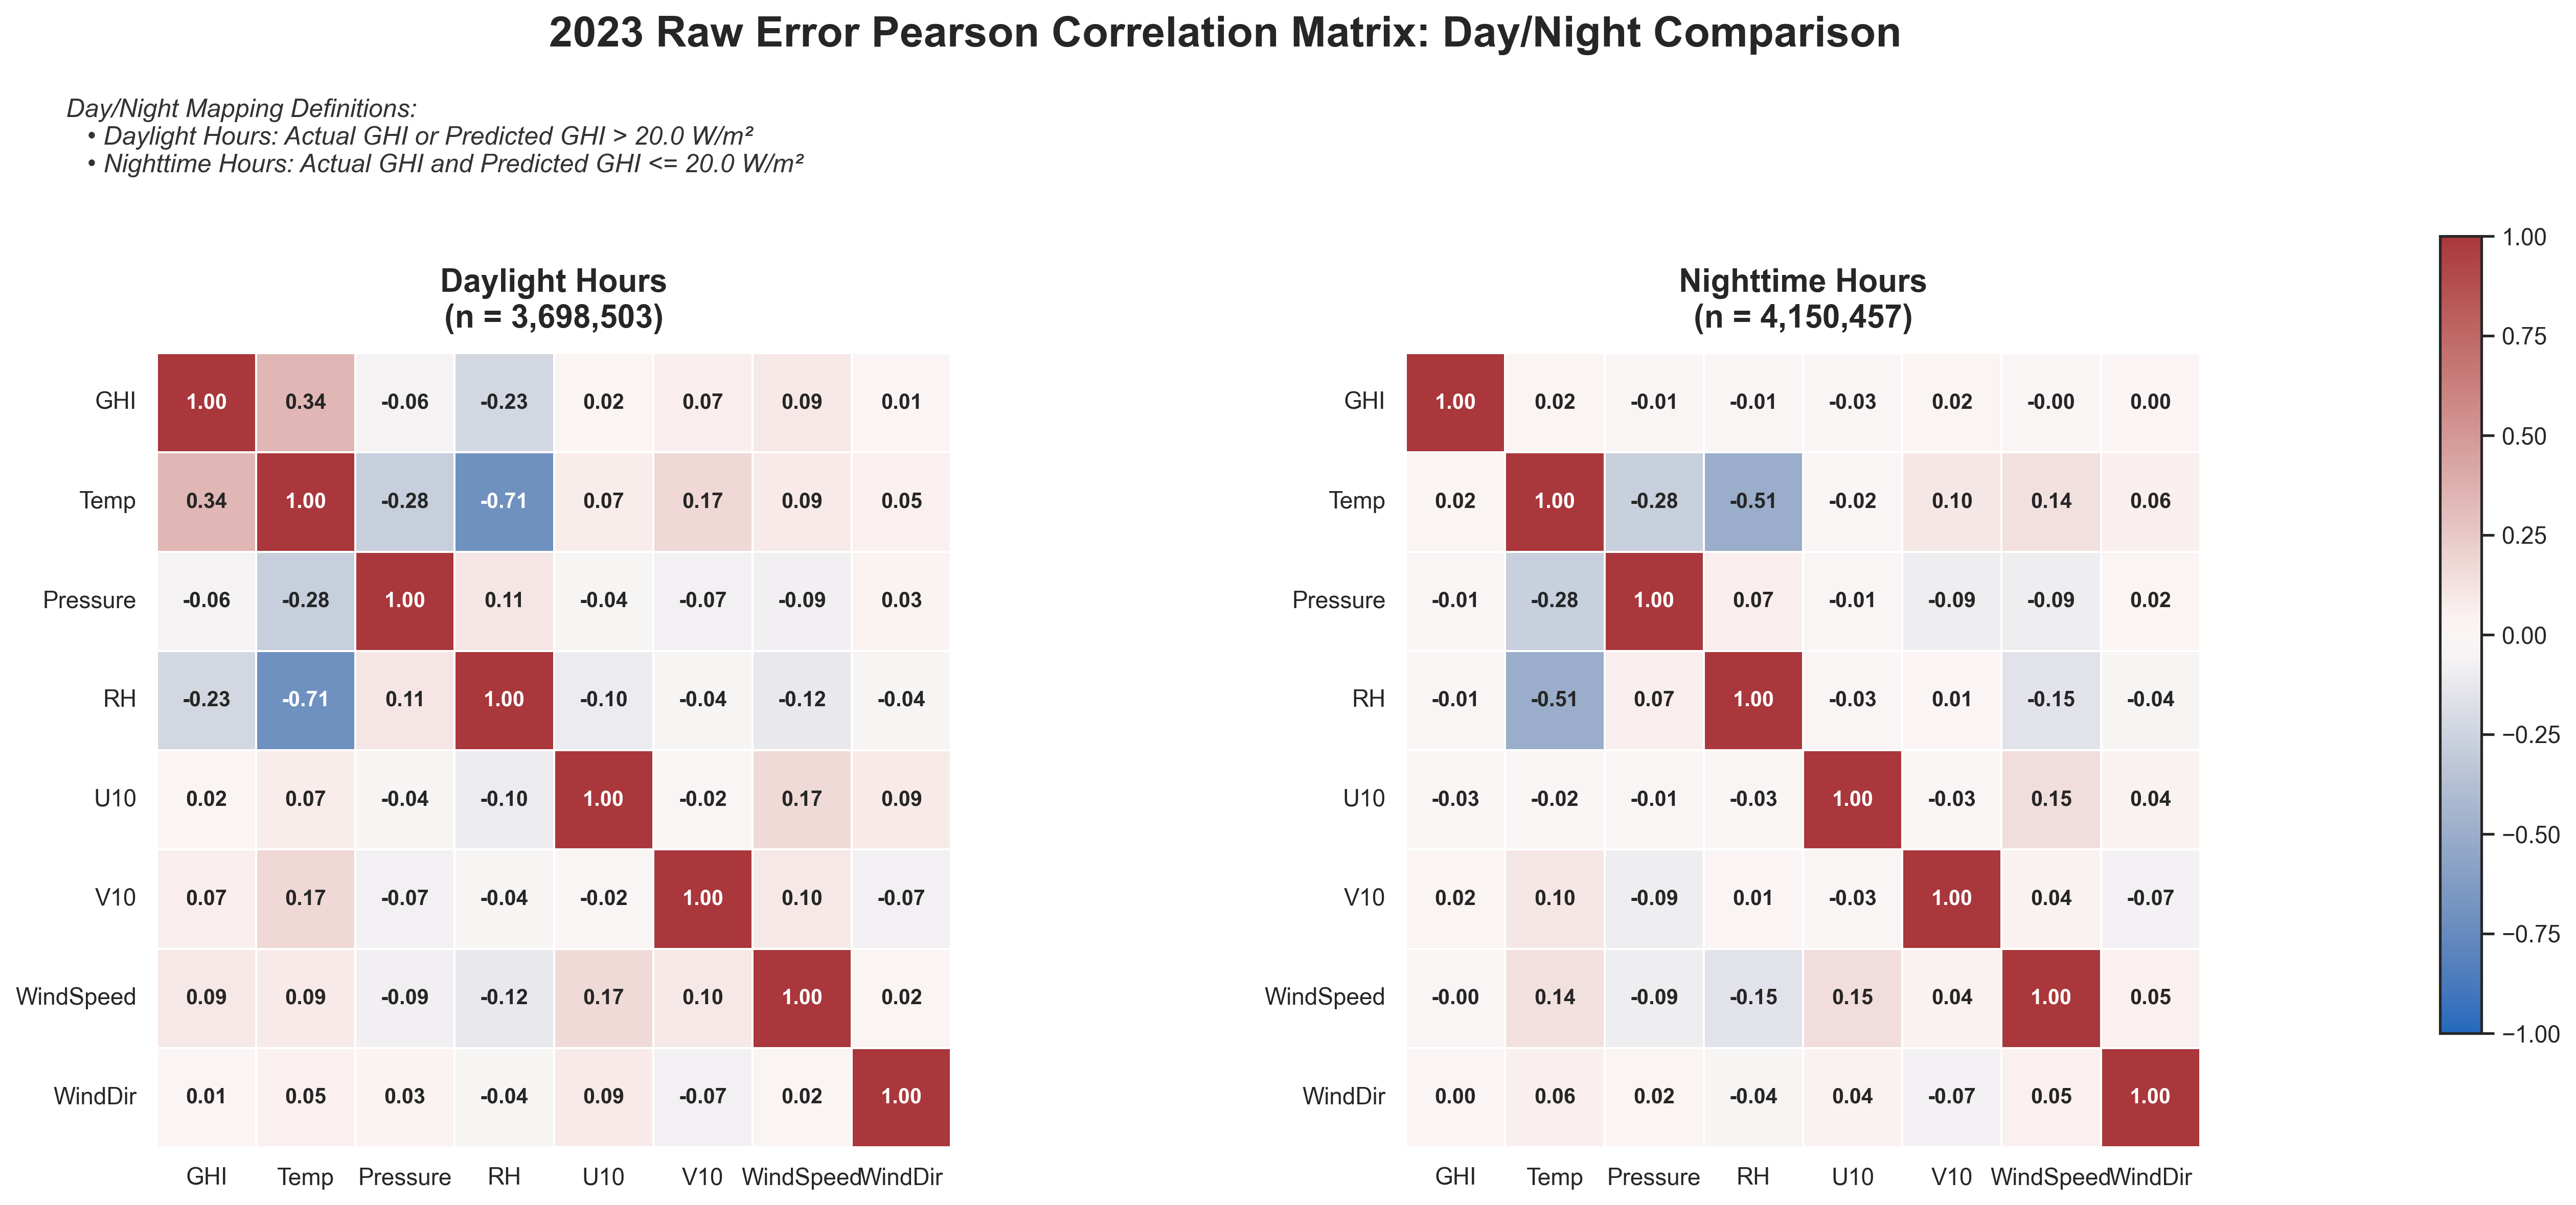
\includegraphics[width=\textwidth]{figures/Q7/YEARS/annual_corr_diurnal_split_2023.png}
  \caption{2023 Raw Error Pearson Correlation Matrix: Daylight Hours ($n = 3,698,503$, left) versus Nighttime Hours ($n = 4,150,457$, right) comparison.}
  \label{fig:app_corr_2023}
\end{figure}

\begin{figure}[H]
  \centering
  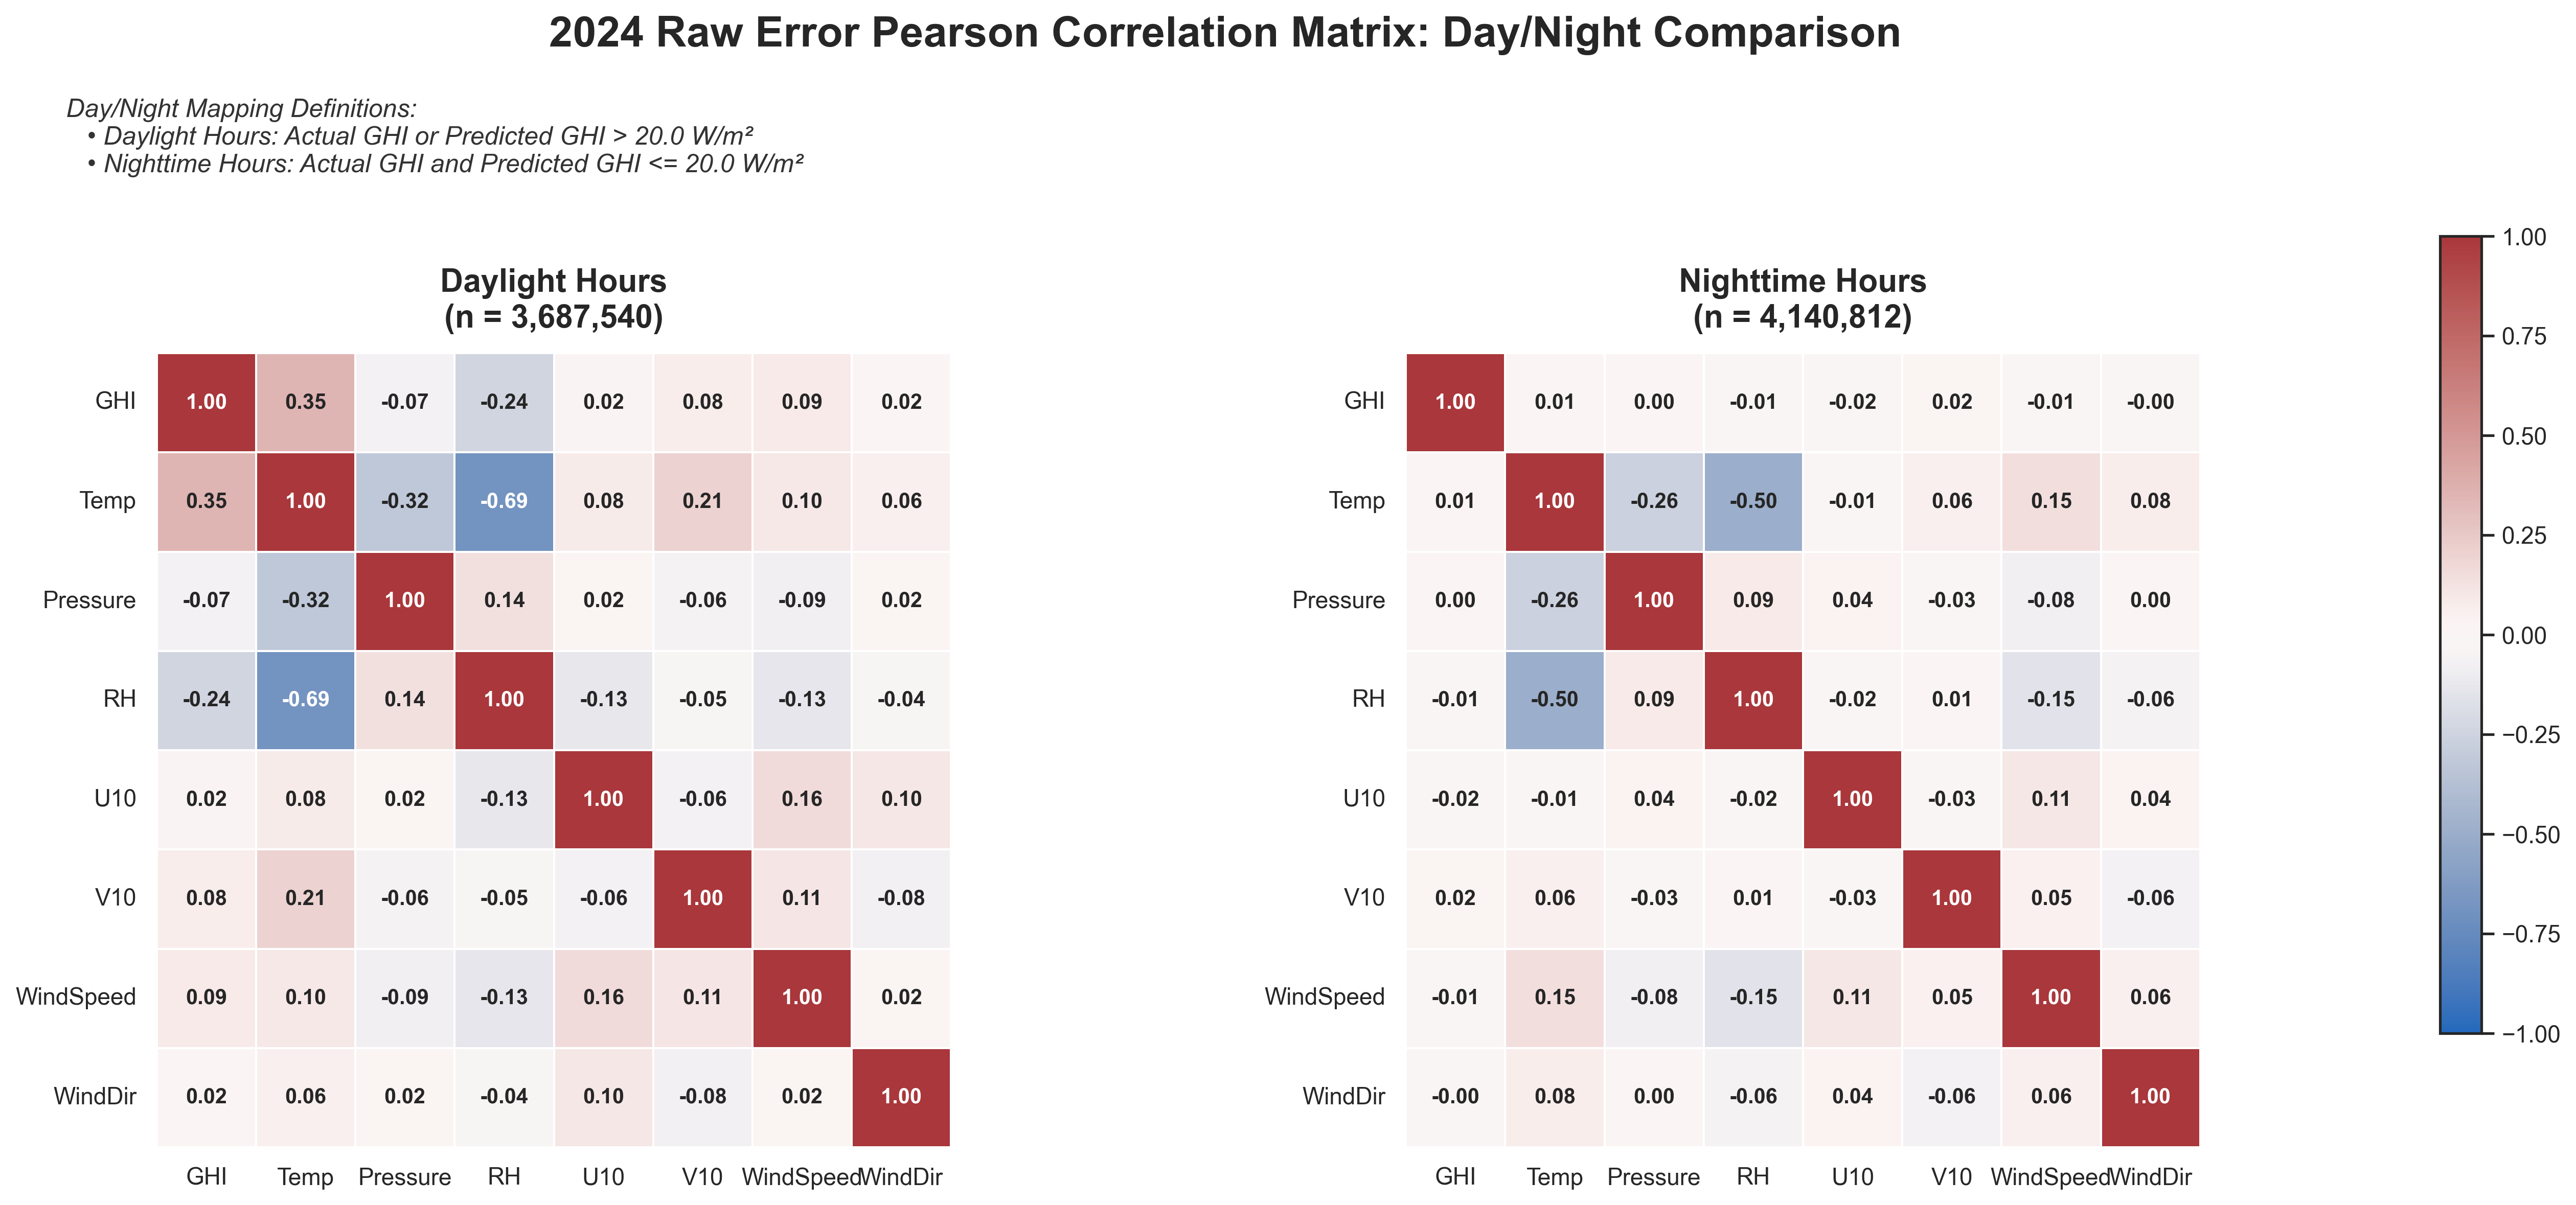
\includegraphics[width=\textwidth]{figures/Q7/YEARS/annual_corr_diurnal_split_2024.png}
  \caption{2024 Raw Error Pearson Correlation Matrix: Daylight Hours ($n = 3,687,540$, left) versus Nighttime Hours ($n = 4,140,812$, right) comparison.}
  \label{fig:app_corr_2024}
\end{figure}

% --- REGIONAL / ZONAL VARIATIONS ---
\begin{figure}[H]
  \centering
  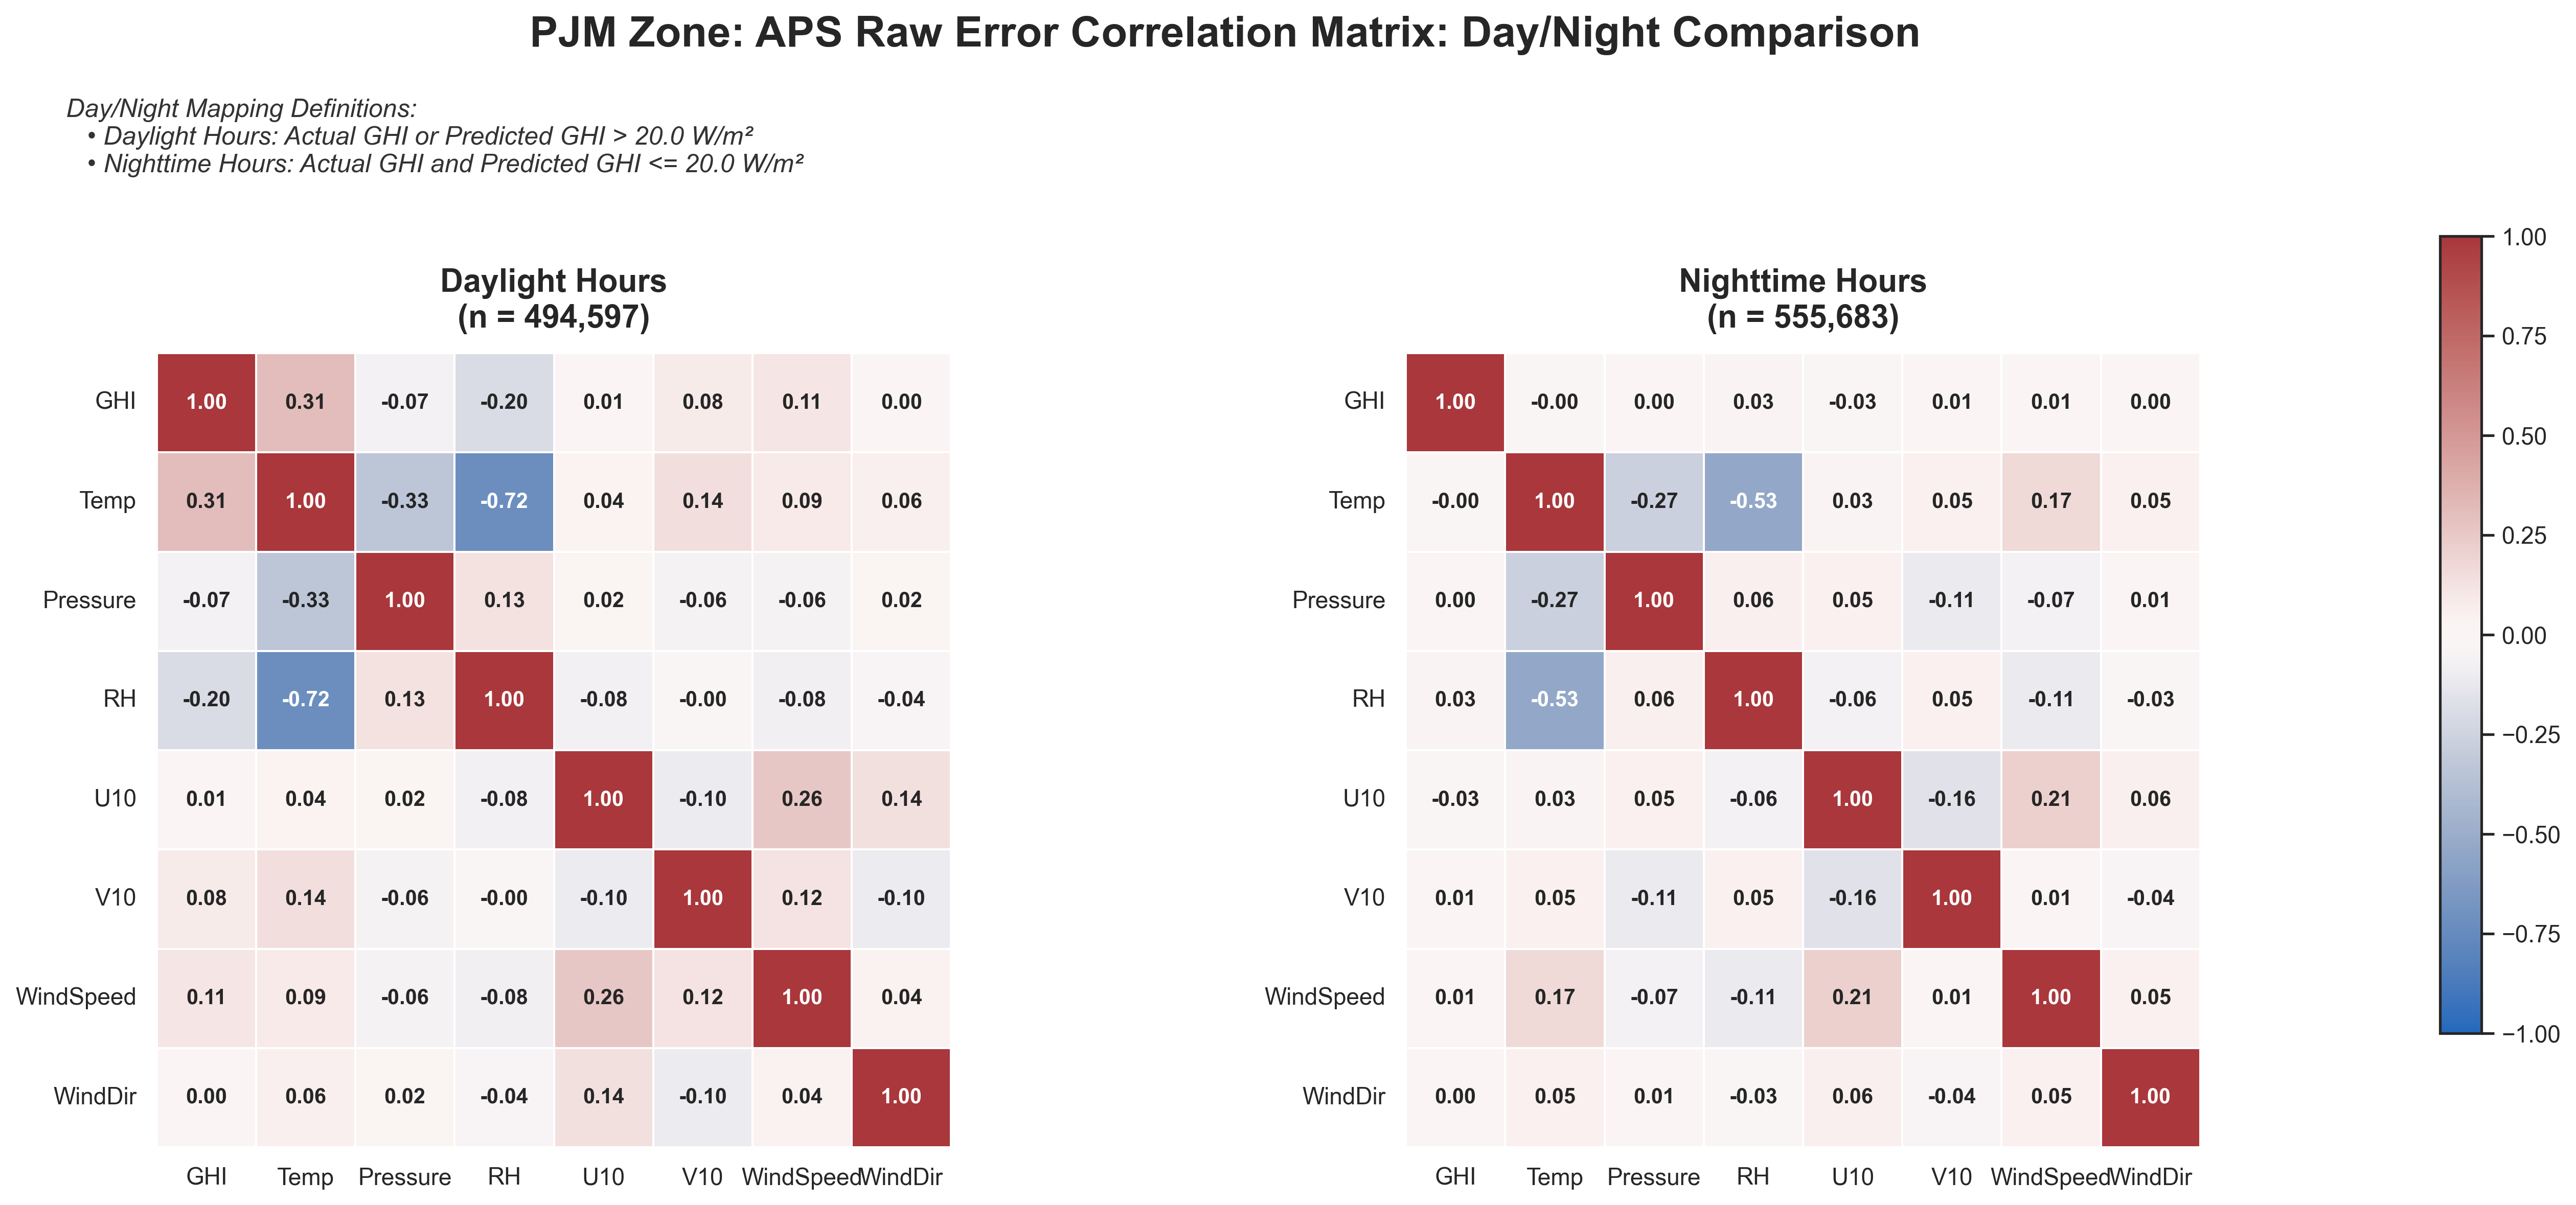
\includegraphics[width=\textwidth]{figures/Q7/ZONES/zone_corr_diurnal_split_aps.png}
  \caption{Cross-variable error matrices computed independently across major PJM transmission zones.}
  \label{fig:app_zone_aps}
\end{figure}

\begin{figure}[H]
  \centering
  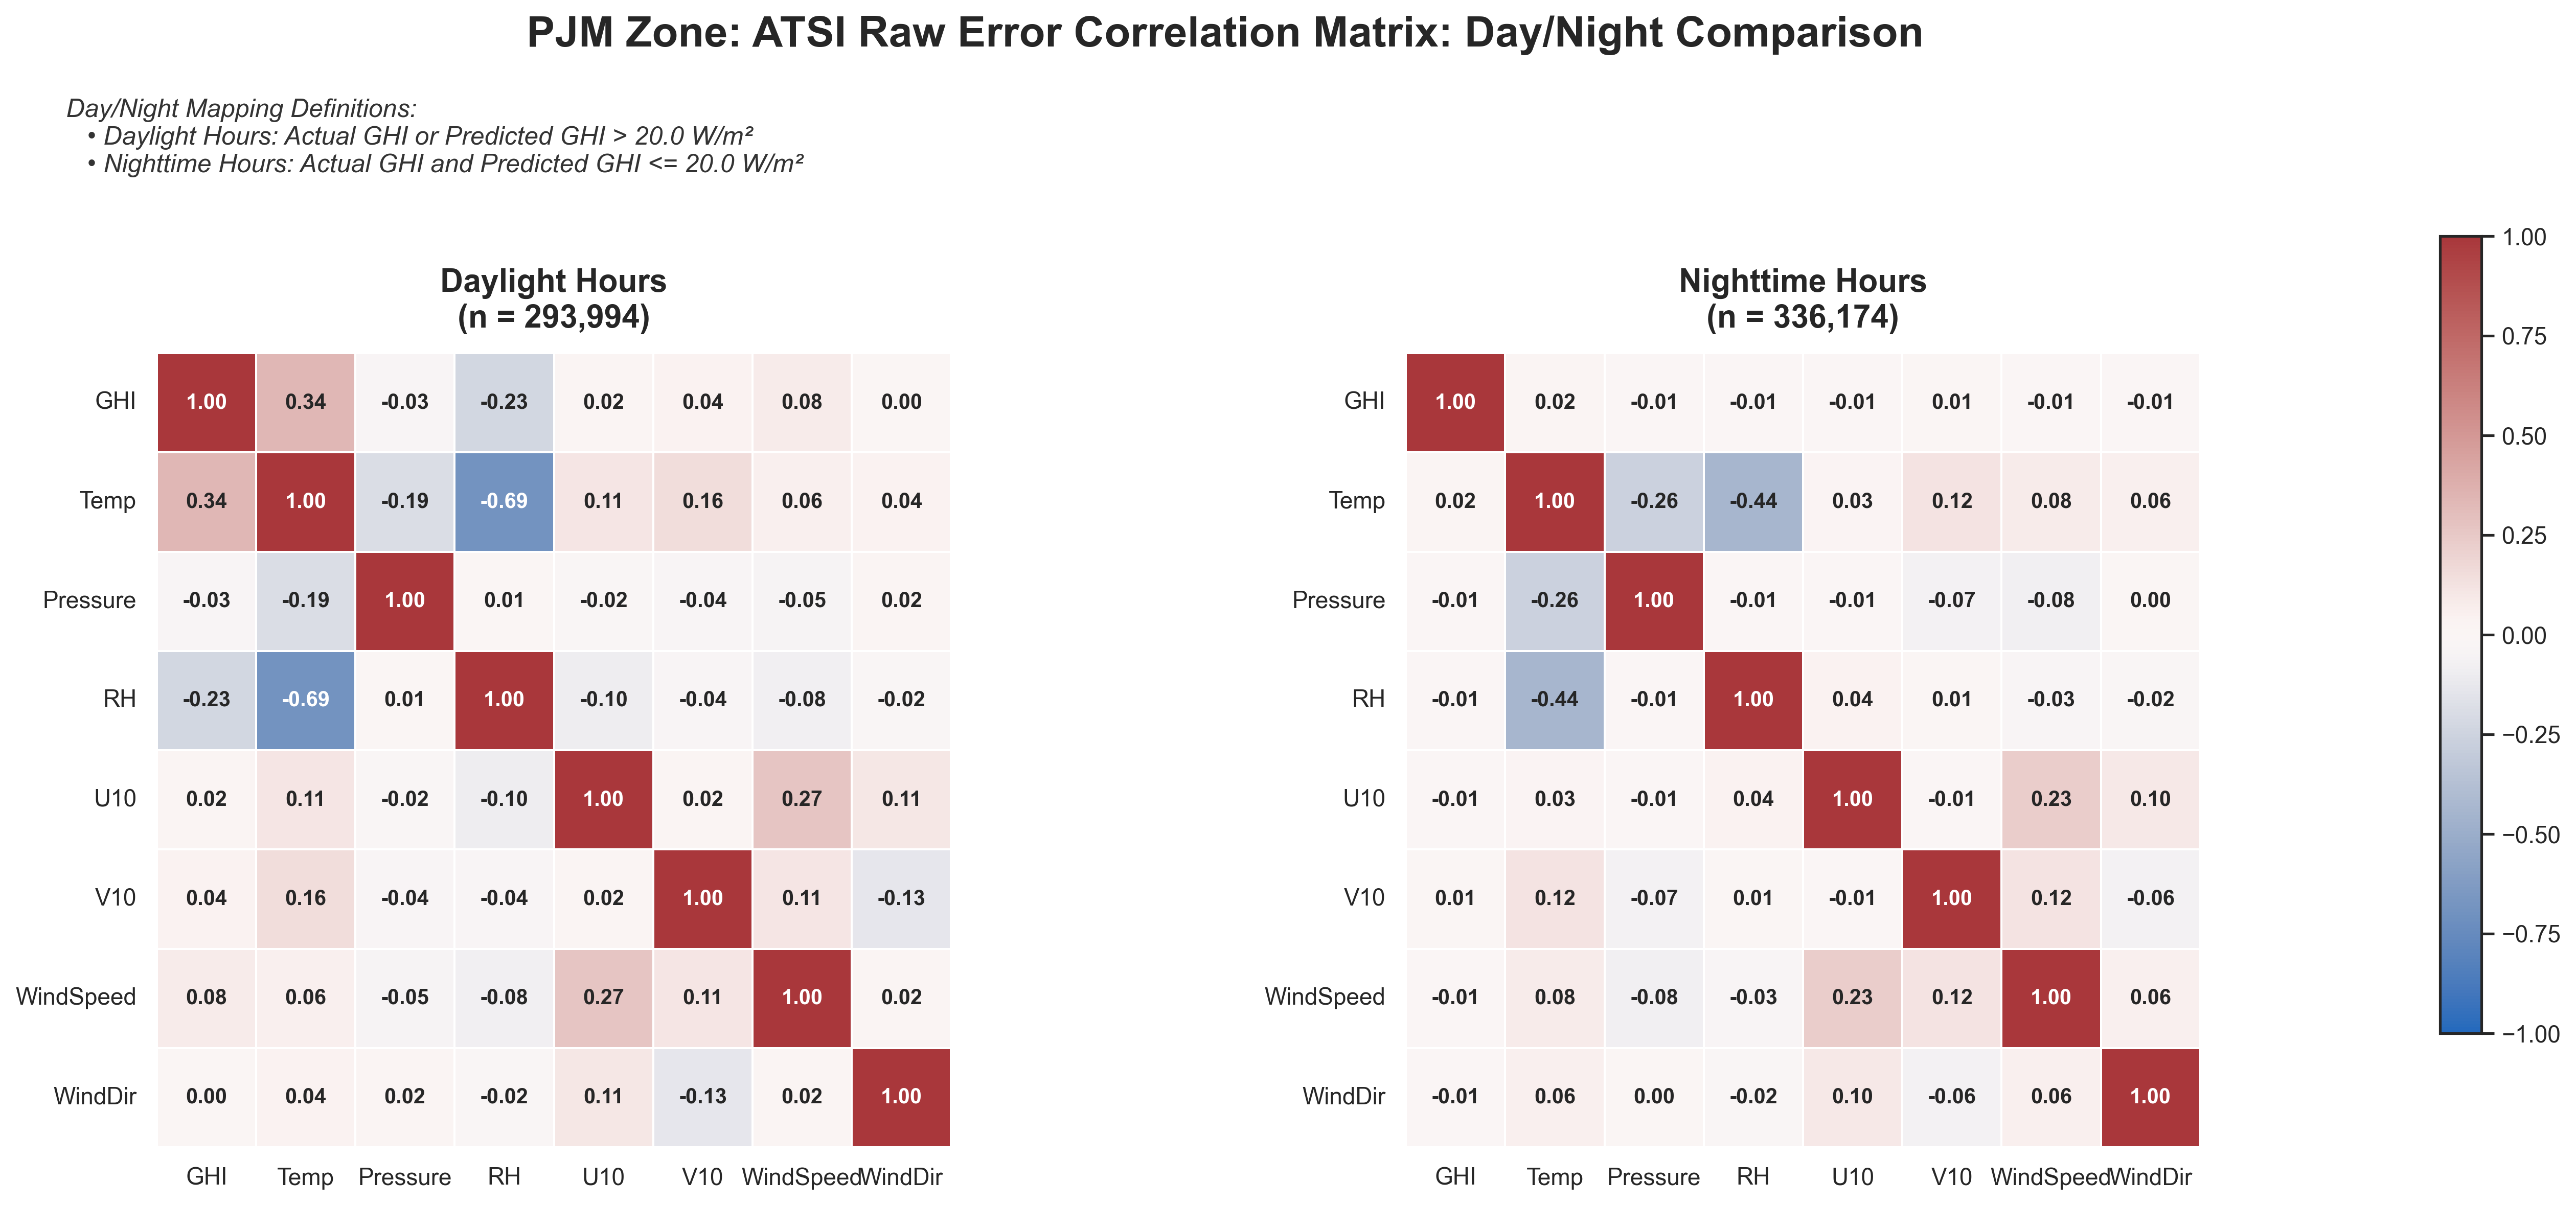
\includegraphics[width=\textwidth]{figures/Q7/ZONES/zone_corr_diurnal_split_atsi.png}
  \caption{Cross-variable error matrices computed independently across major PJM transmission zones.}
  \label{fig:app_zone_atsi}
\end{figure}

\begin{figure}[H]
  \centering
  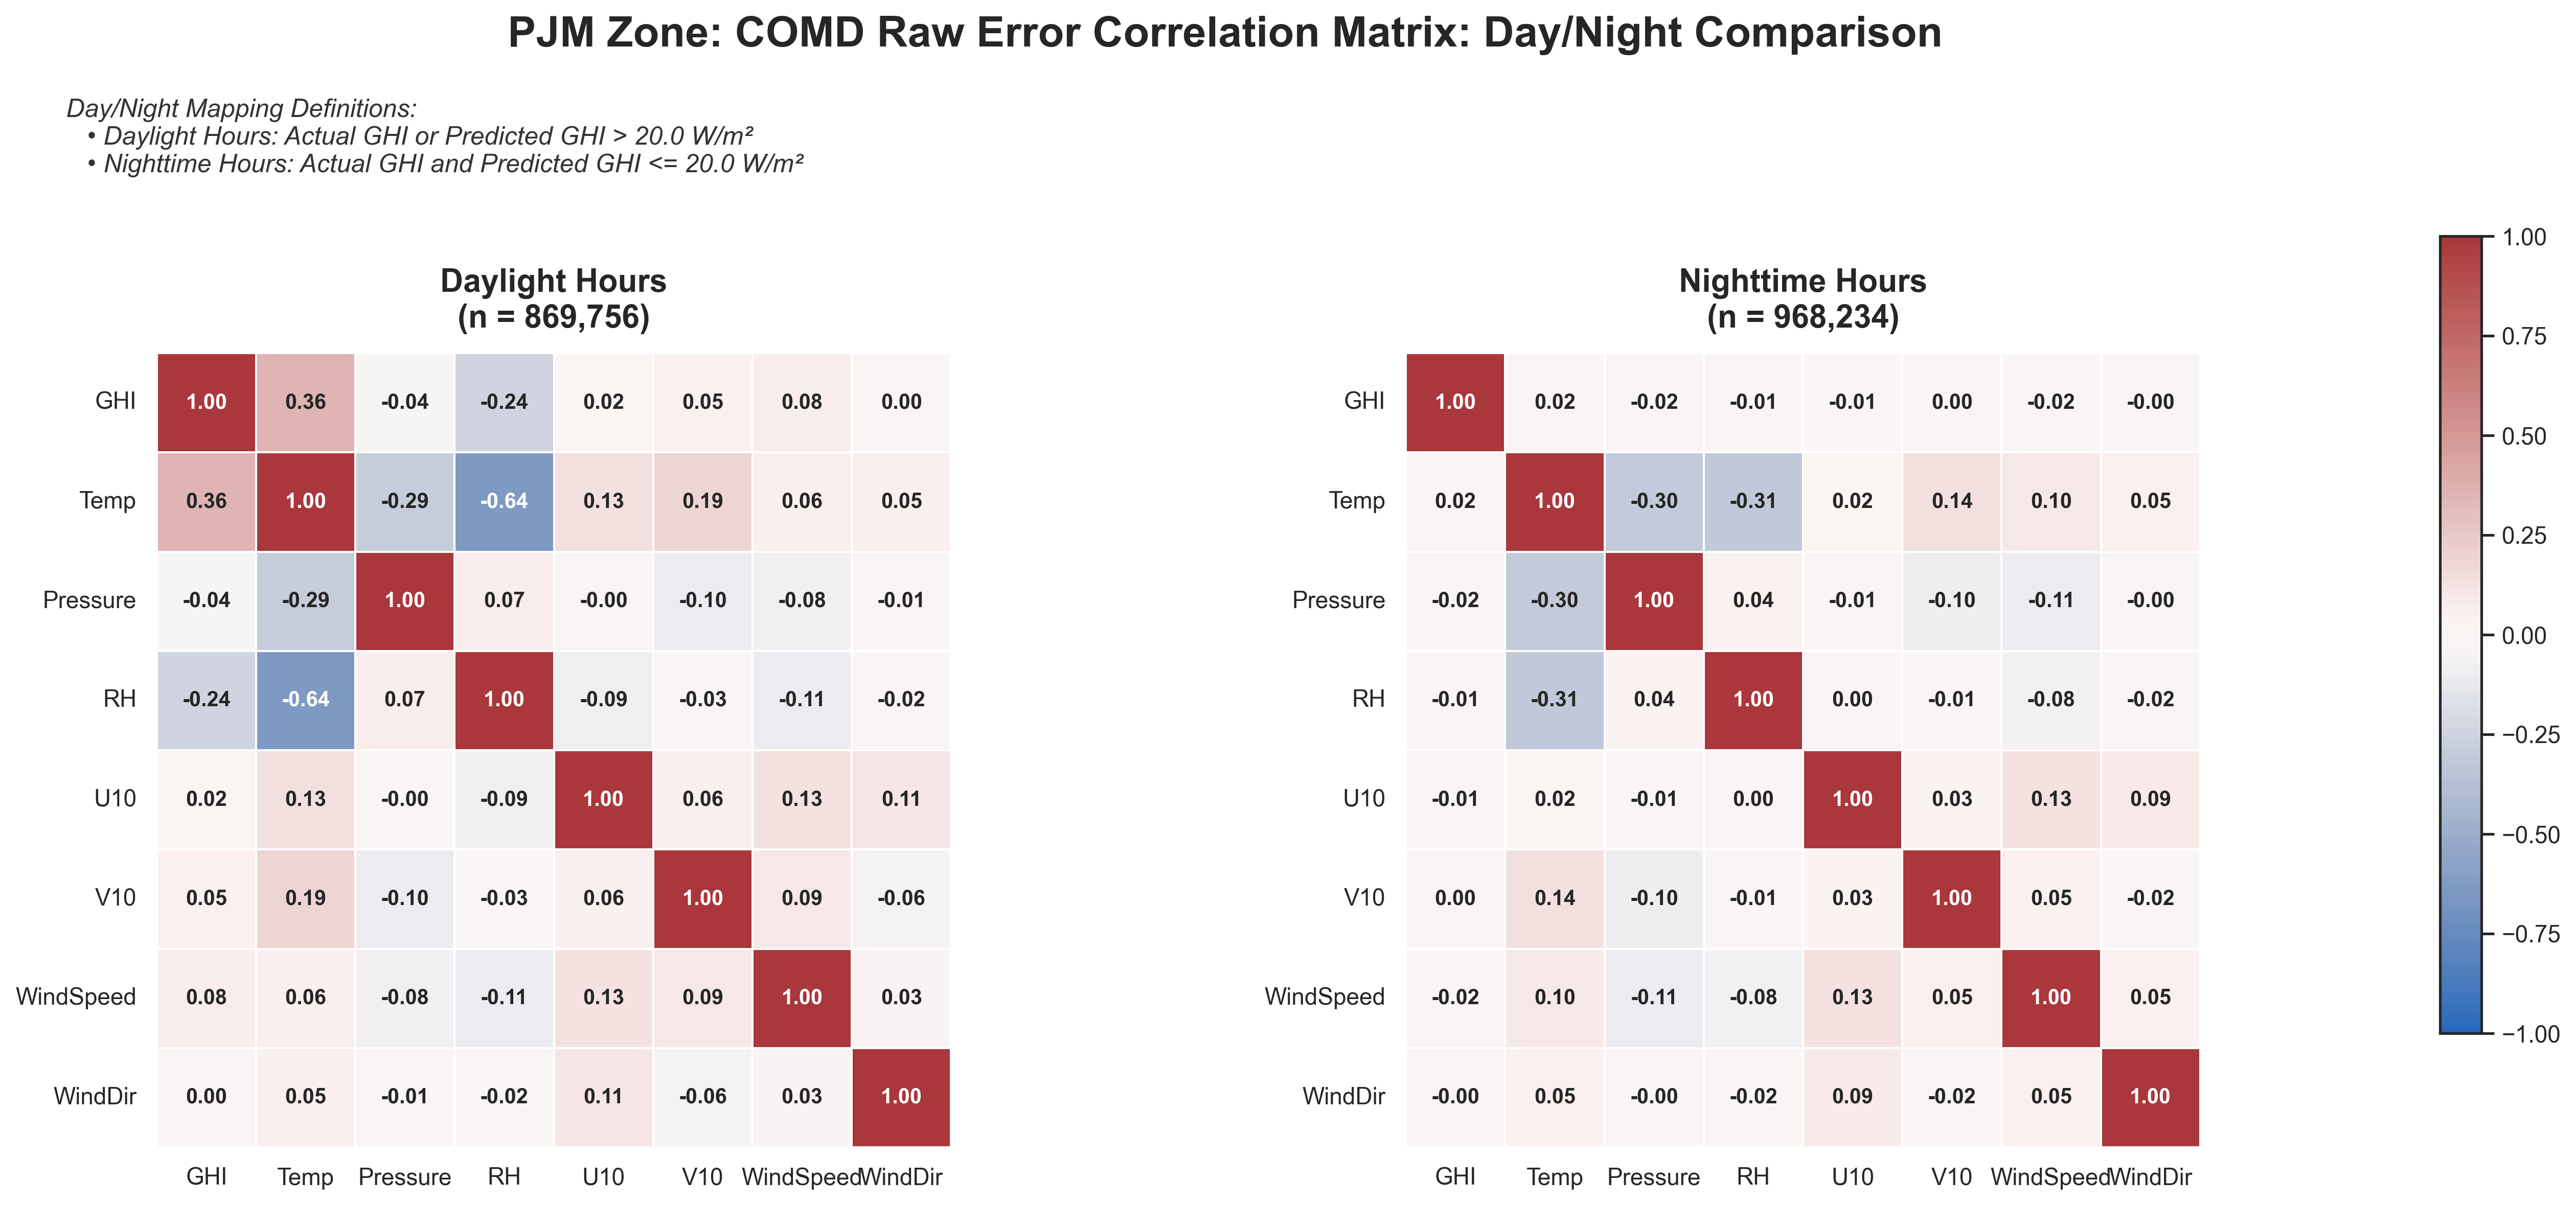
\includegraphics[width=\textwidth]{figures/Q7/ZONES/zone_corr_diurnal_split_comd.png}
  \caption{Cross-variable error matrices computed independently across major PJM transmission zones.}
  \label{fig:app_zone_comd}
\end{figure}

\begin{figure}[H]
  \centering
  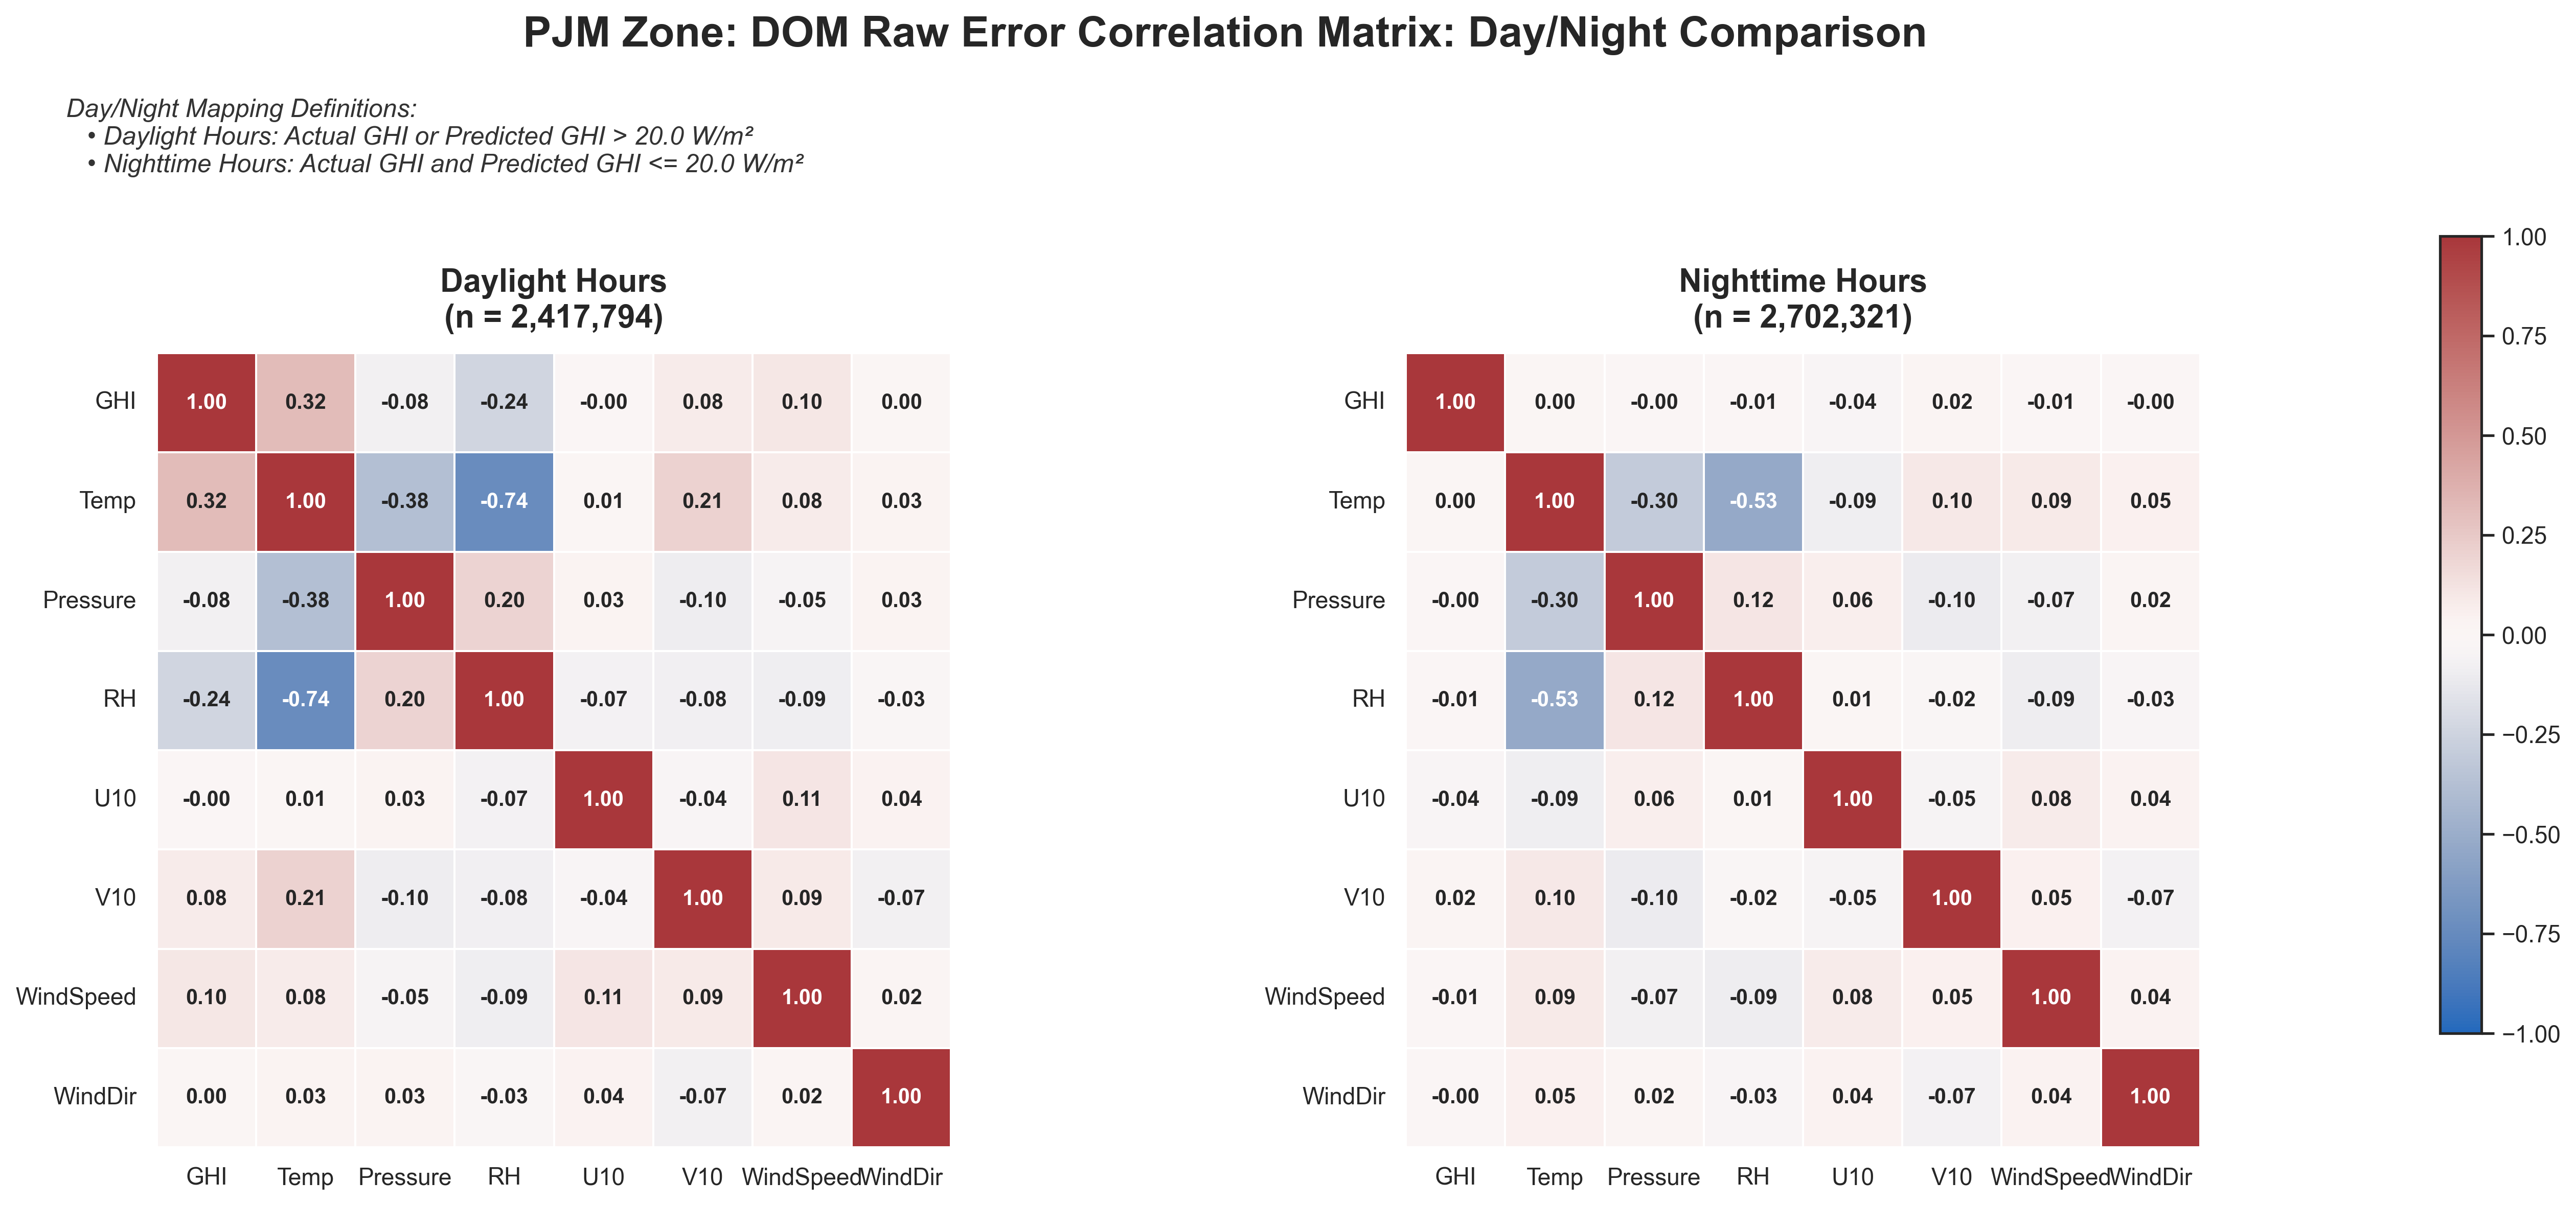
\includegraphics[width=\textwidth]{figures/Q7/ZONES/zone_corr_diurnal_split_dom.png}
  \caption{Cross-variable error matrices computed independently across major PJM transmission zones.}
  \label{fig:app_zone_dom}
\end{figure}

\begin{figure}[H]
  \centering
  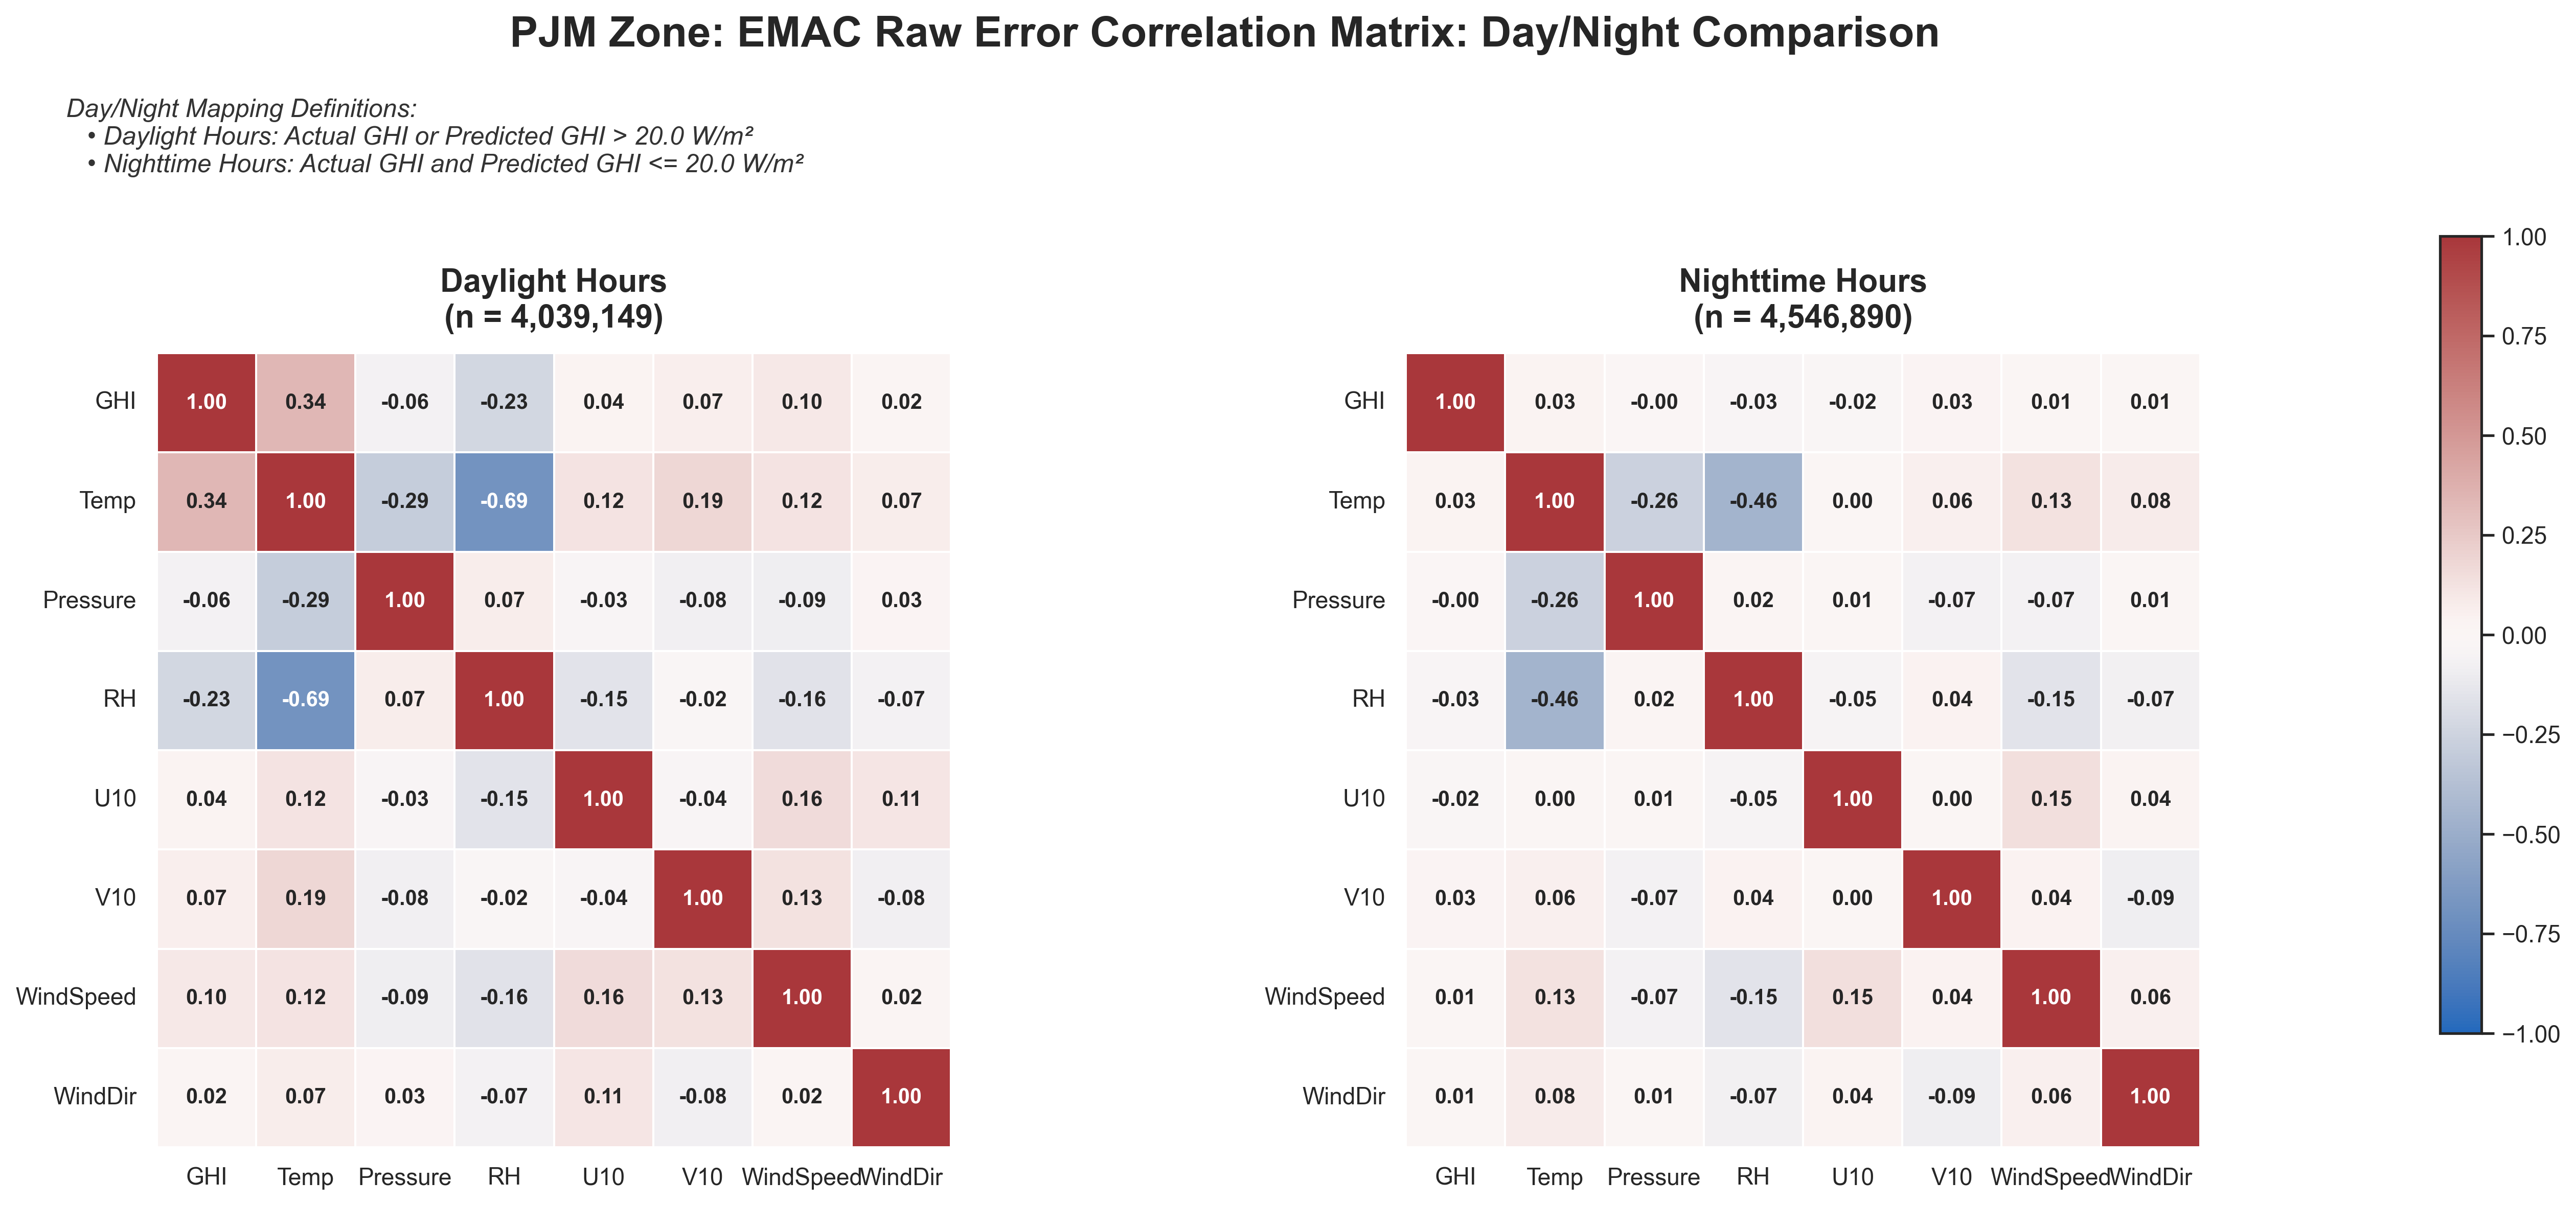
\includegraphics[width=\textwidth]{figures/Q7/ZONES/zone_corr_diurnal_split_emac.png}
  \caption{Cross-variable error matrices computed independently across major PJM transmission zones.}
  \label{fig:app_zone_emac}
\end{figure}

\begin{figure}[H]
  \centering
  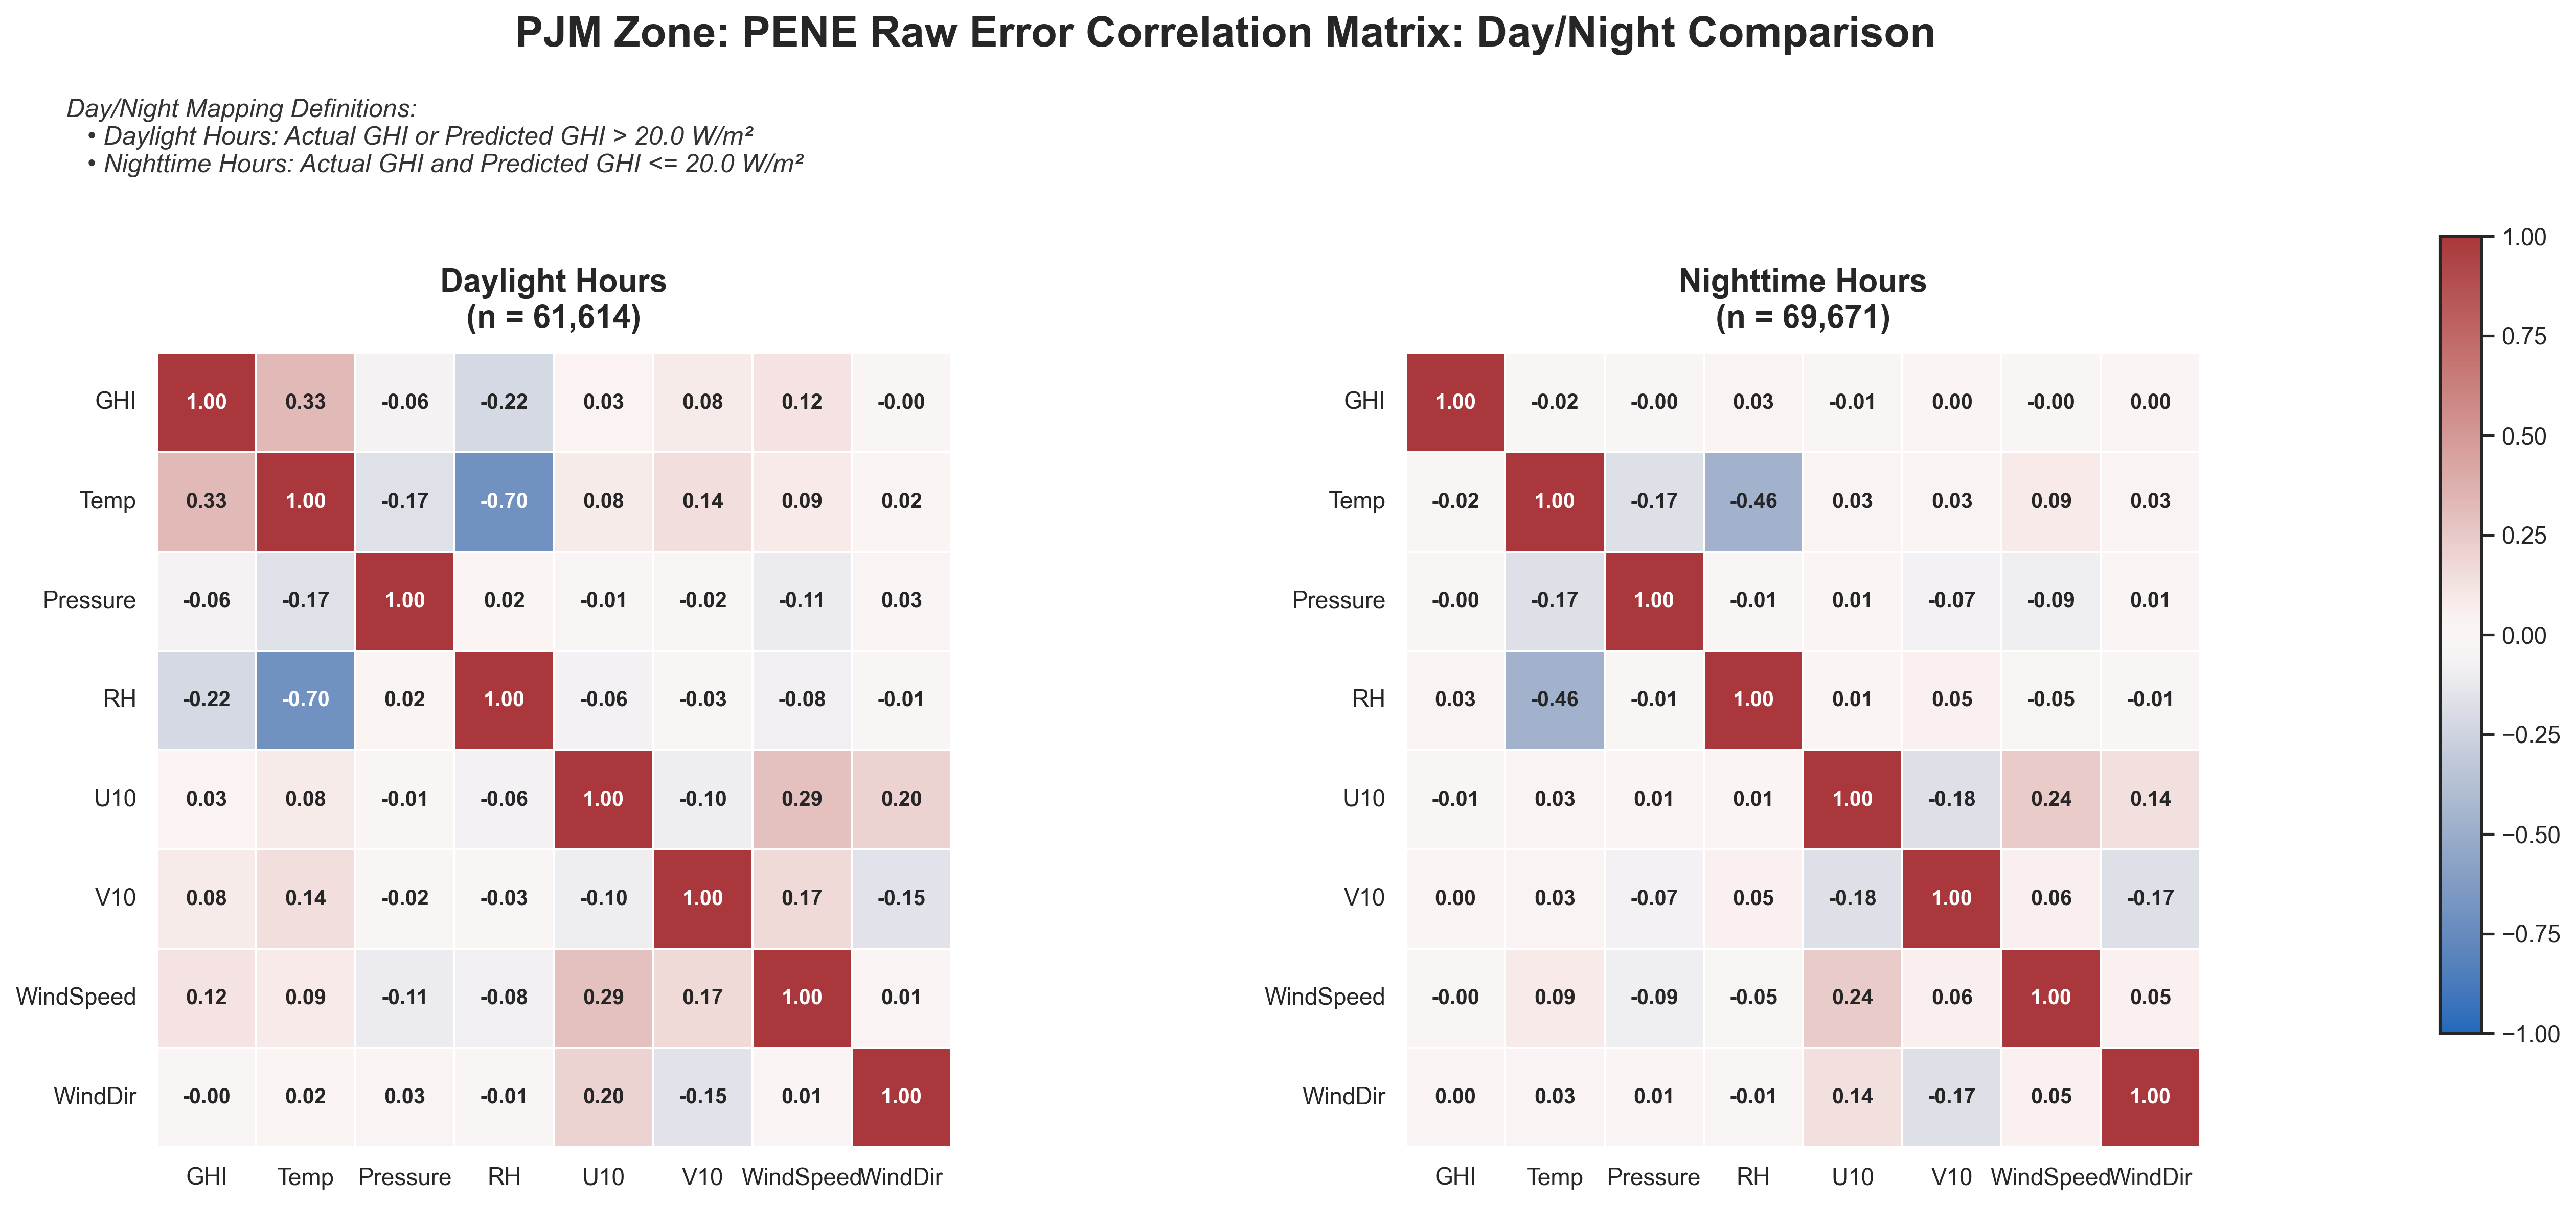
\includegraphics[width=\textwidth]{figures/Q7/ZONES/zone_corr_diurnal_split_pene.png}
  \caption{Cross-variable error matrices computed independently across major PJM transmission zones.}
  \label{fig:app_zone_pene}
\end{figure}

\begin{figure}[H]
  \centering
  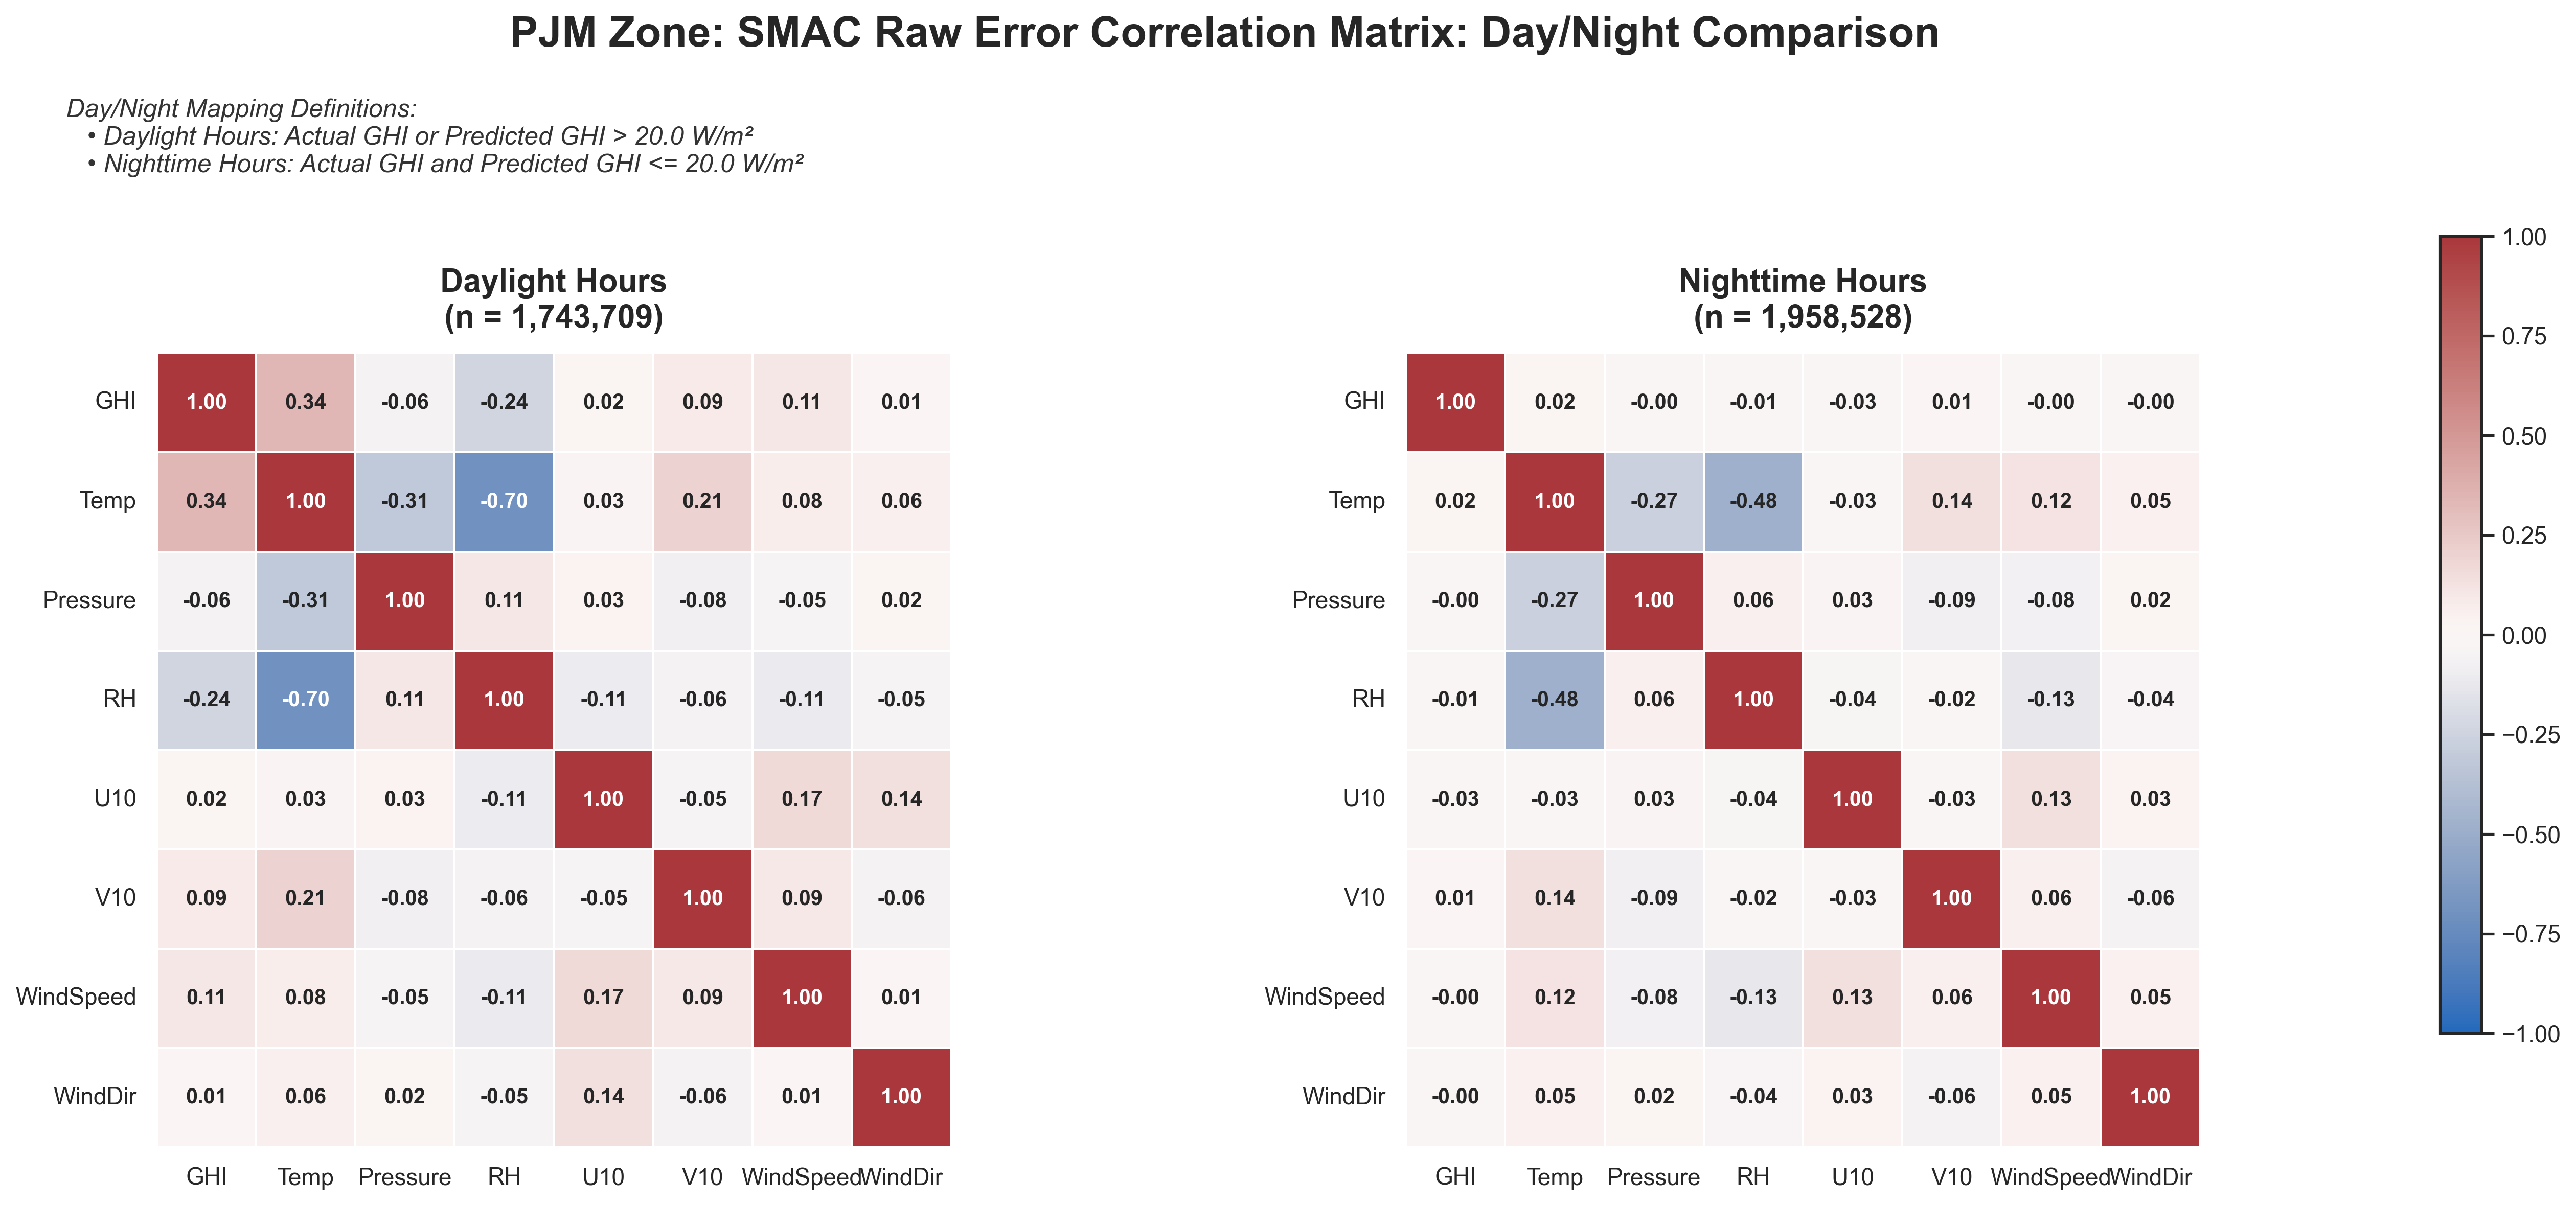
\includegraphics[width=\textwidth]{figures/Q7/ZONES/zone_corr_diurnal_split_smac.png}
  \caption{Cross-variable error matrices computed independently across major PJM transmission zones.}
  \label{fig:app_zone_smac}
\end{figure}

\begin{figure}[H]
  \centering
  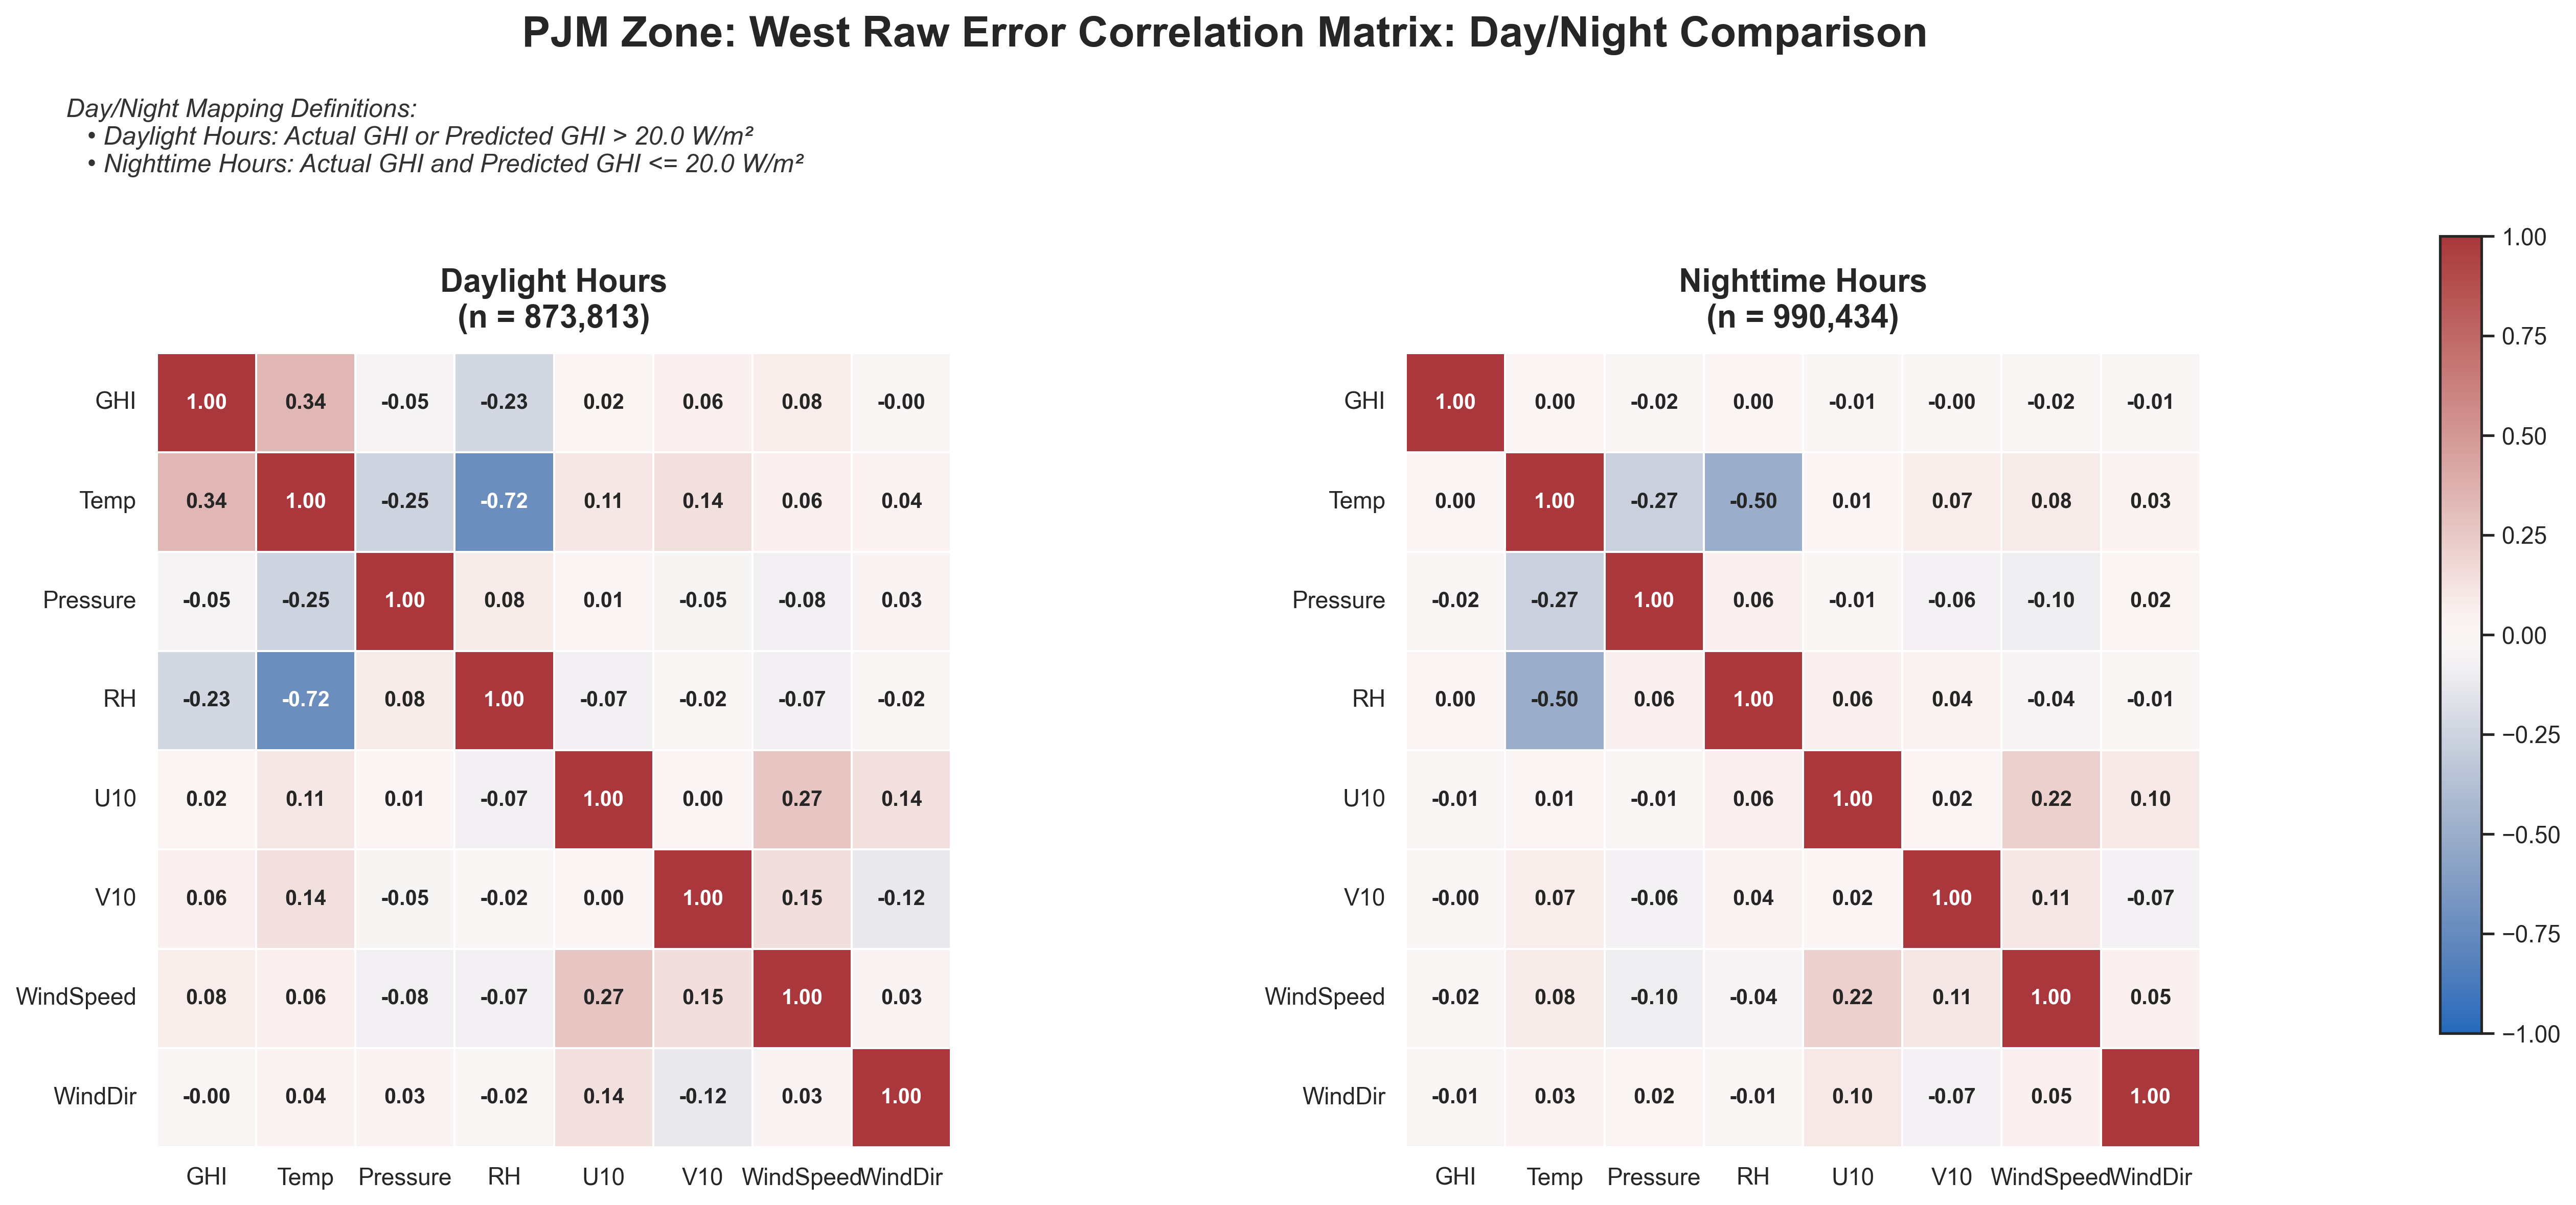
\includegraphics[width=\textwidth]{figures/Q7/ZONES/zone_corr_diurnal_split_west.png}
  \caption{Cross-variable error matrices computed independently across major PJM transmission zones.}
  \label{fig:app_zone_west}
\end{figure}

\begin{figure}[H]
  \centering
  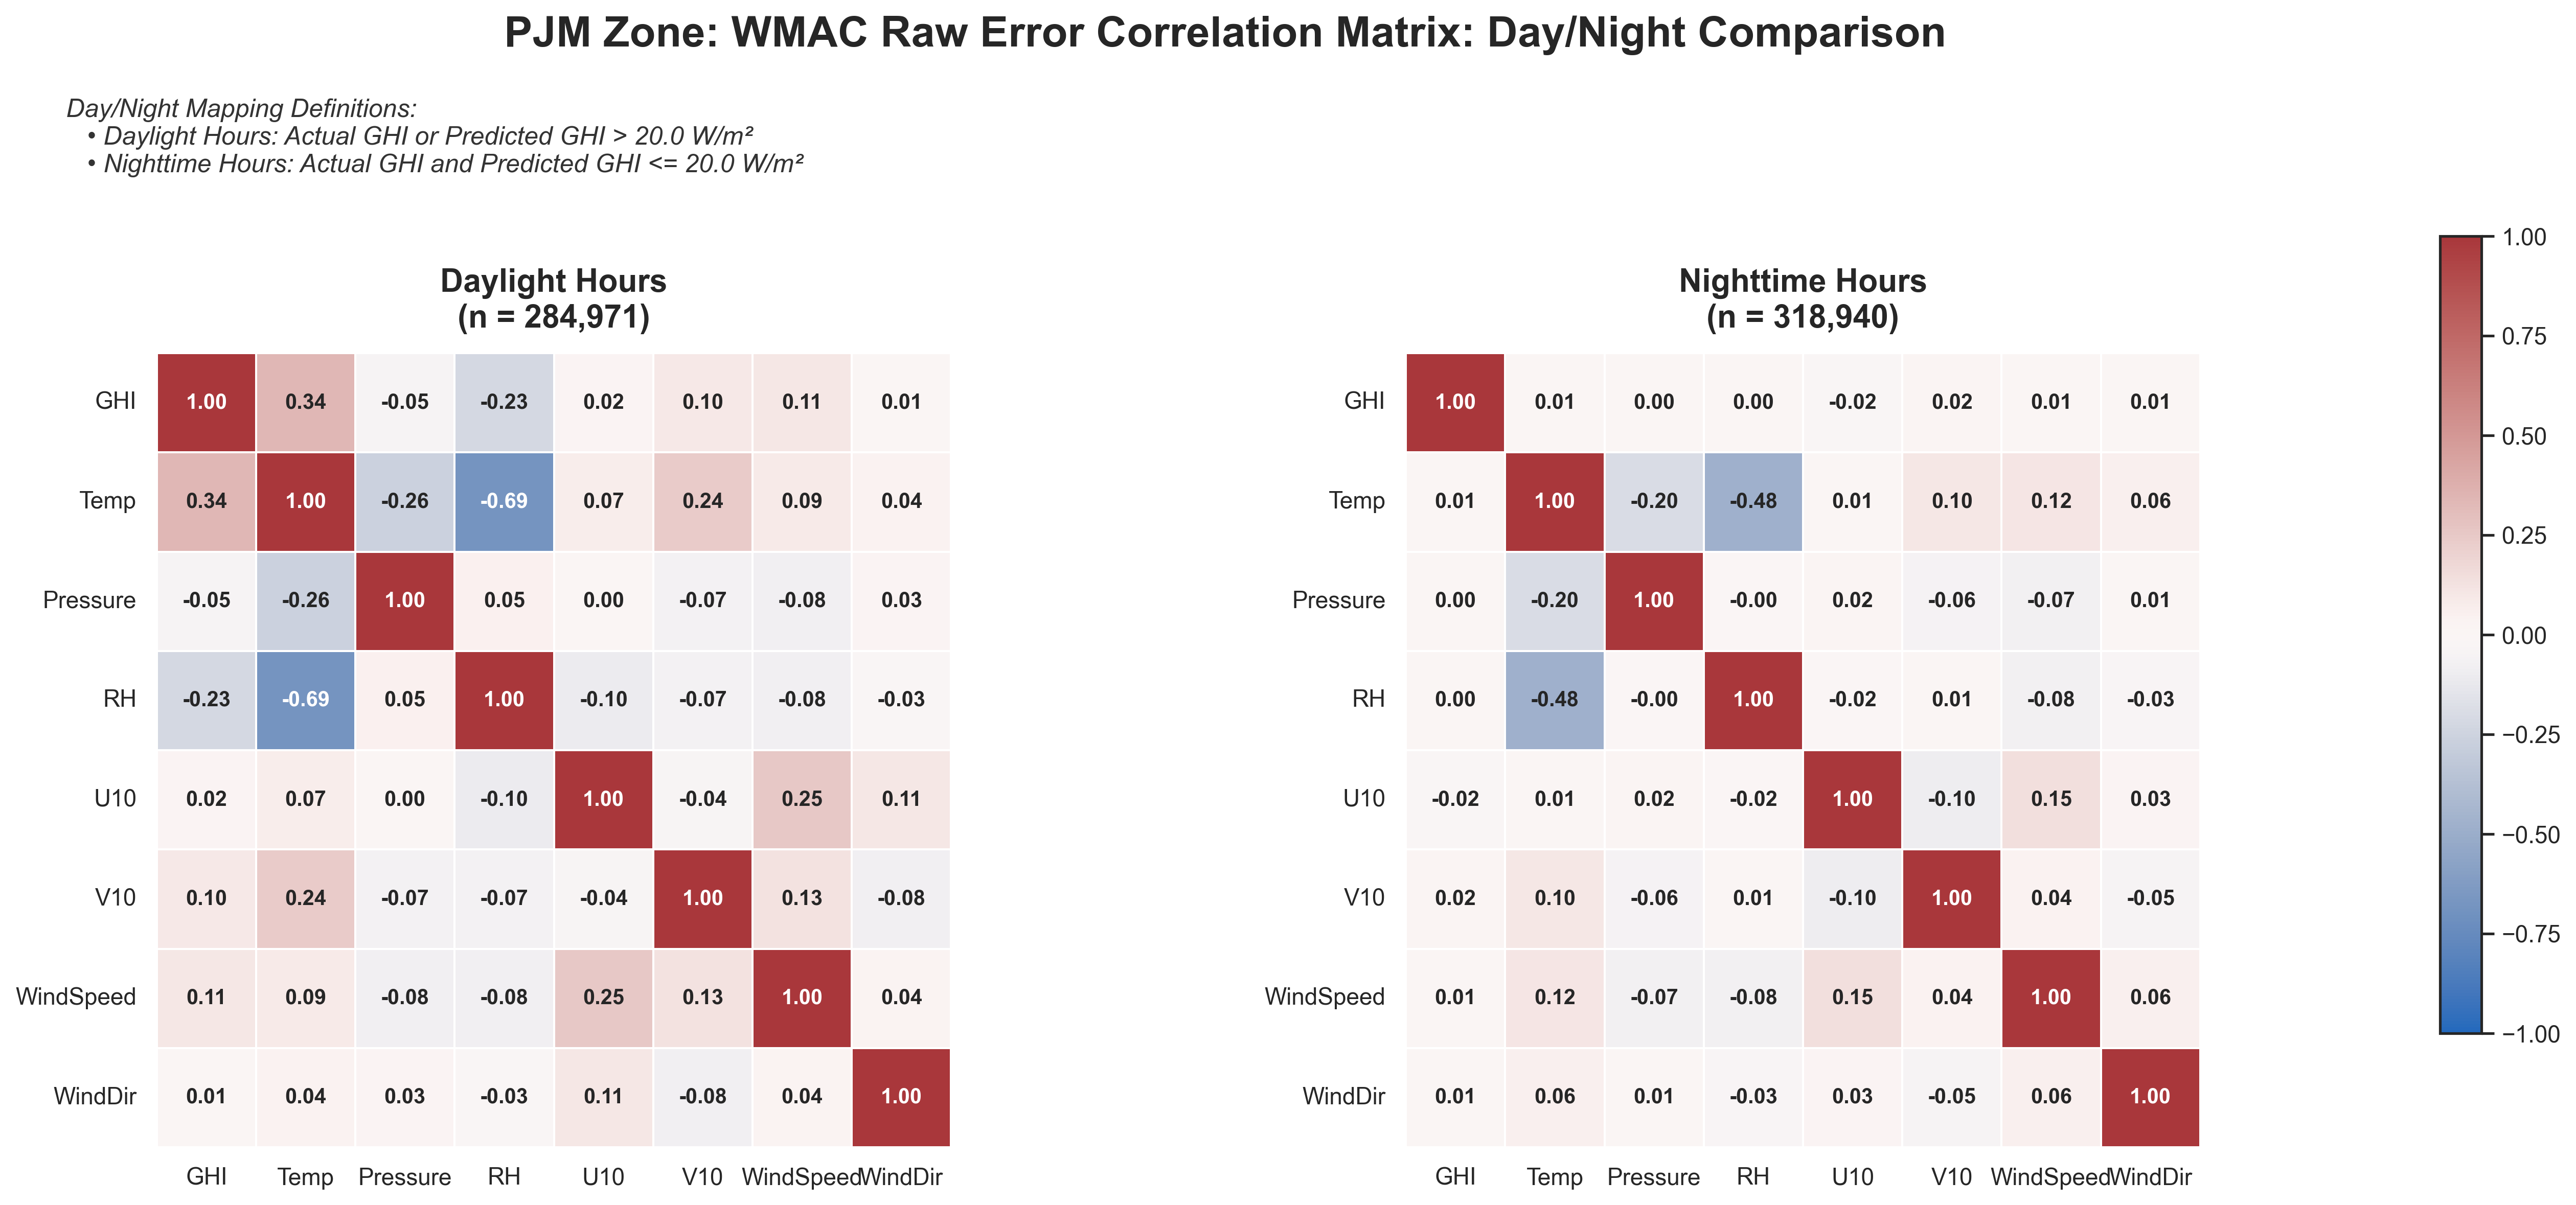
\includegraphics[width=\textwidth]{figures/Q7/ZONES/zone_corr_diurnal_split_wmac.png}
  \caption{Cross-variable error matrices computed independently across major PJM transmission zones.}
  \label{fig:app_zone_wmac}
\end{figure}


\subsection {Q8 — Spatial Correlation Across PJM Zones}

\begin{figure}[H]
  \centering
  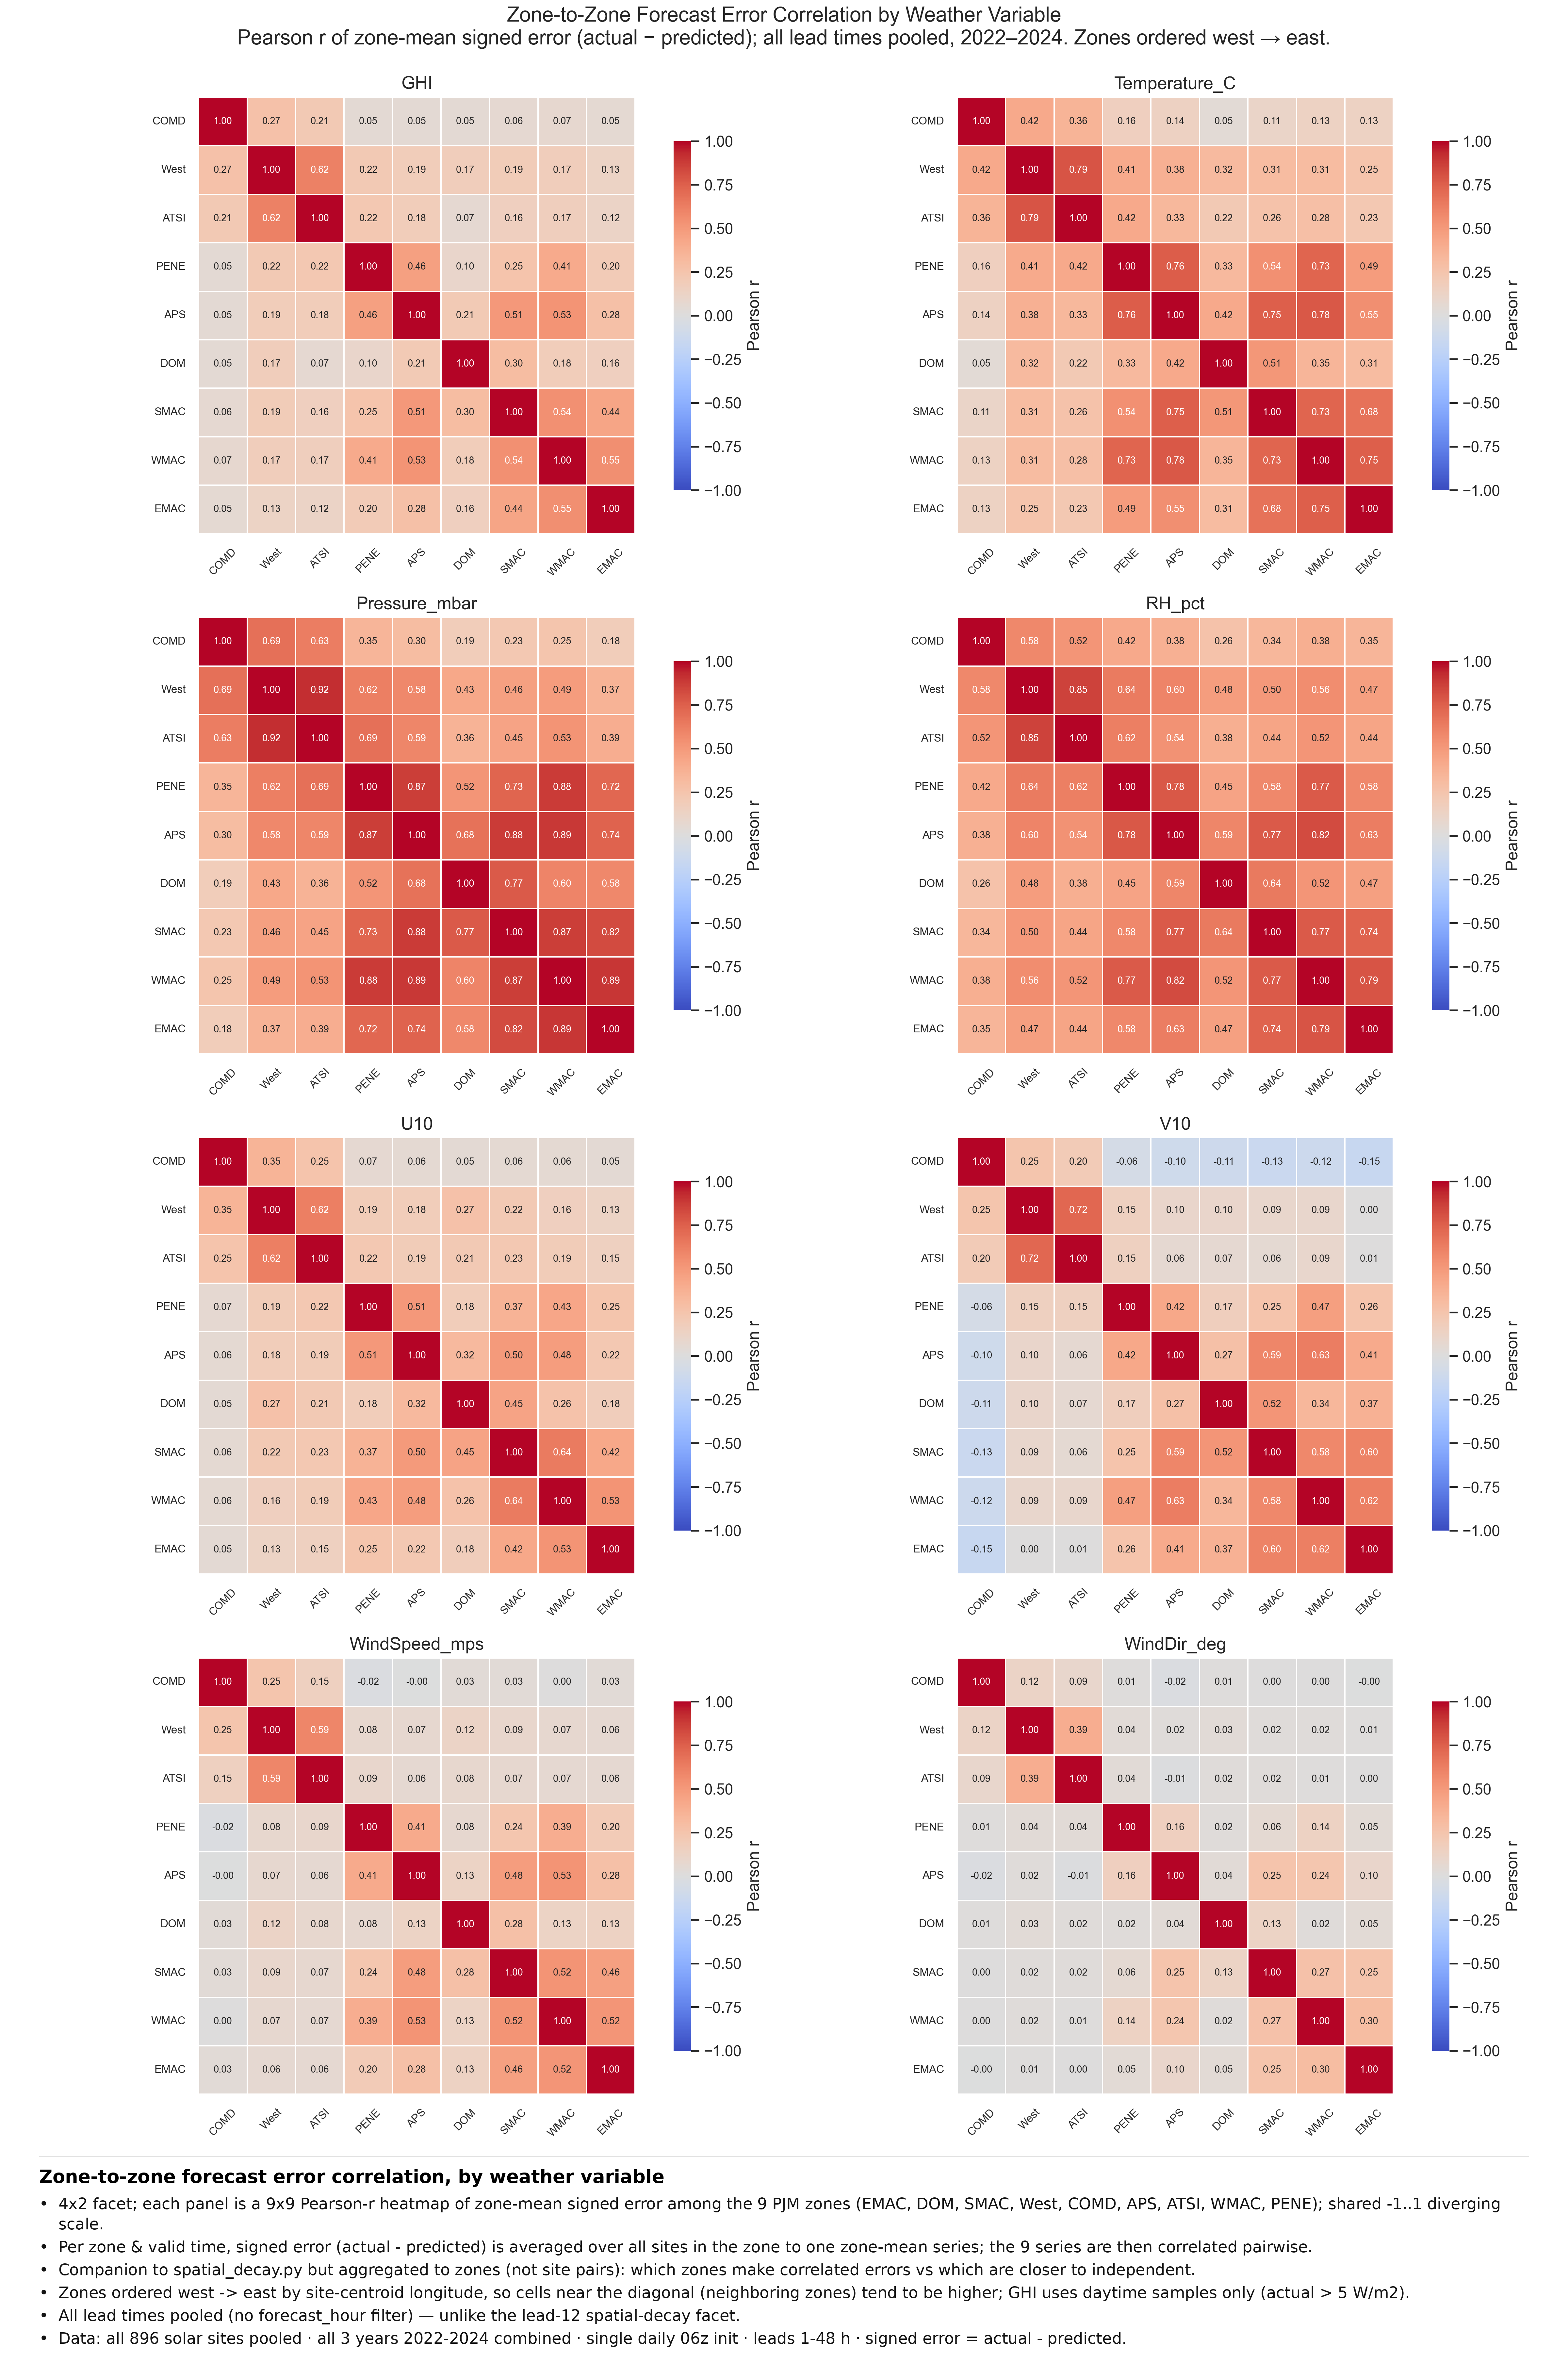
\includegraphics[width=\textwidth]{figures/Q8/zone_error_correlation.png}
  \caption{Complete (all-variable) version of the zone-to-zone forecast-error correlation matrices.}
  \label{fig:app_zonecorr}
\end{figure}

\begin{figure}[H]
  \centering
  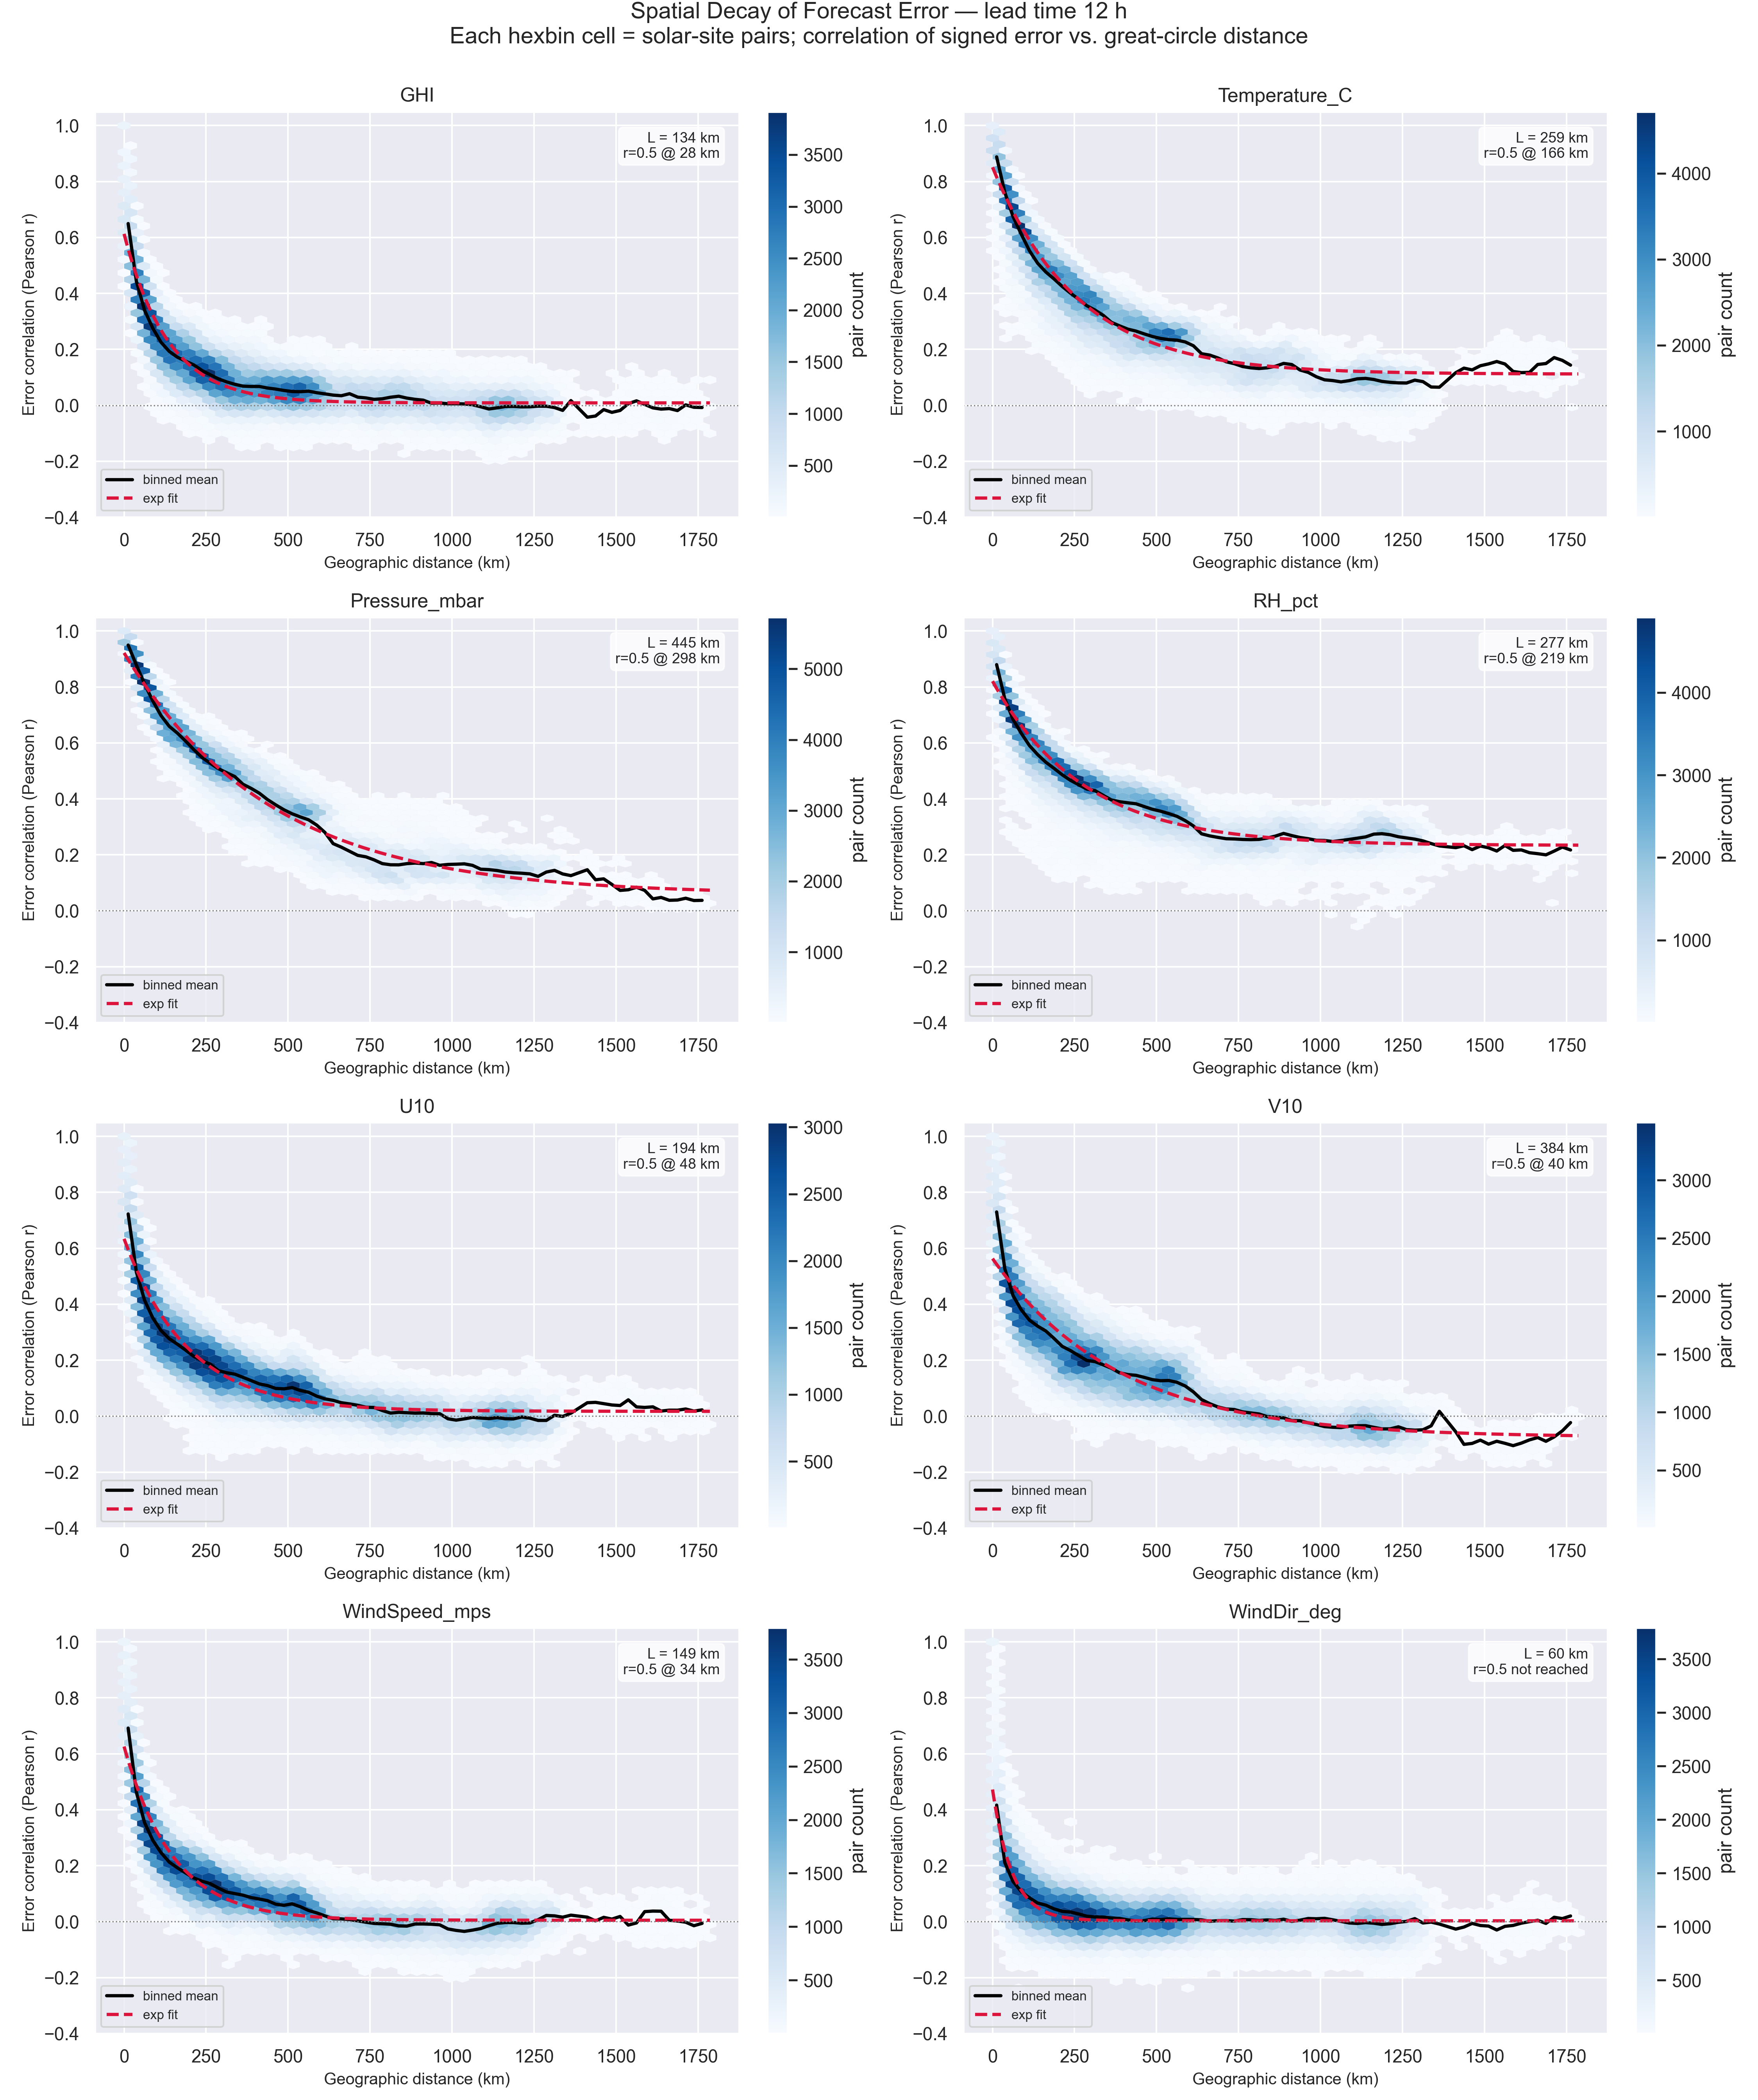
\includegraphics[width=\textwidth]{figures/Q8/spatial_decay_lead12.png}
  \caption{Spatial decay of forecast error at lead~12~h (= \texttt{18z}, solar noon). Each panel
  plots error correlation versus great-circle distance for all $\approx\num{400000}$ site pairs
  (hexbin density), with the distance-binned mean (black) and fitted exponential
  $\rho(d)=a\,e^{-d/L}+c$ (crimson). Pressure is the most spatially coherent
  ($L \approx \SI{445}{km}$); temperature ($L \approx \SI{233}{km}$) and RH
  ($L \approx \SI{277}{km}$) are intermediate; GHI decorrelates fastest
  ($L \approx \SI{134}{km}$, $r=0.5$ by $\sim\SI{28}{km}$); wind direction is so noisy its fit
  never reaches $r=0.5$.}
  \label{fig:decay12}
\end{figure}

Sweeping the lead time (Figure~\ref{fig:decaylead}) shows how both the \emph{reach} ($L$) and the
\emph{strength} of correlation evolve.

\begin{figure}[H]
  \centering
  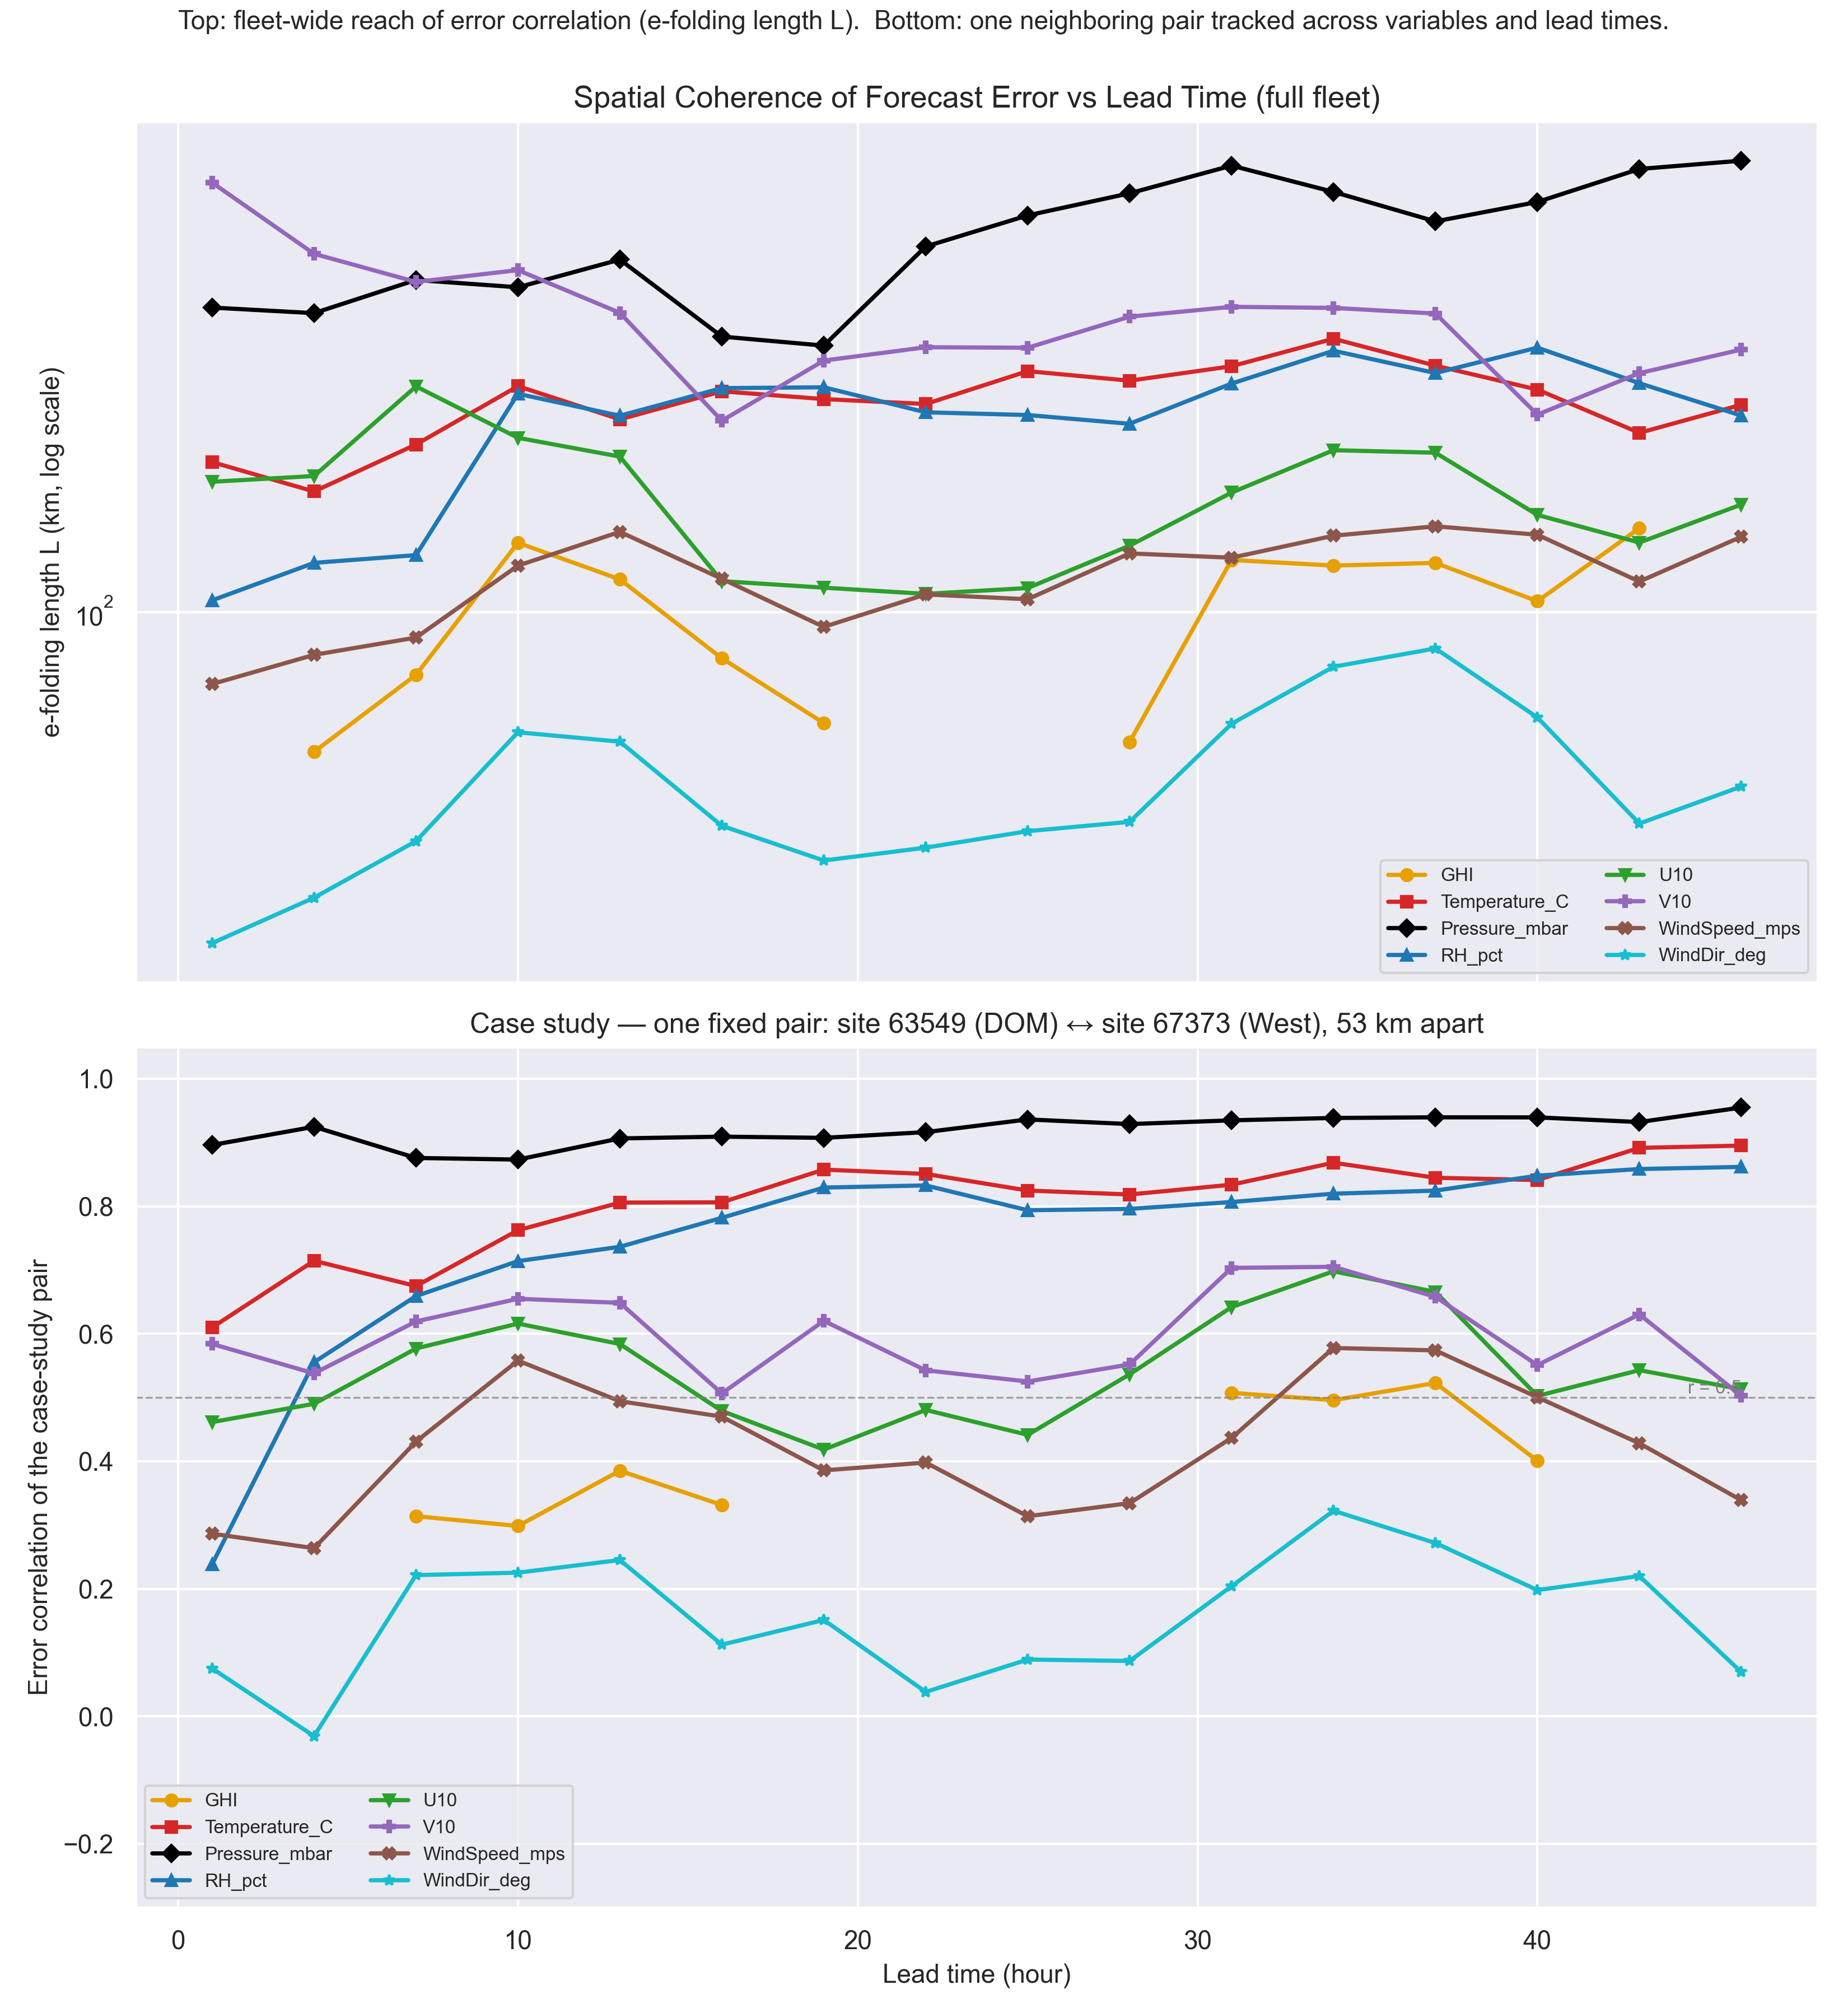
\includegraphics[width=\textwidth]{figures/Q8/decorrelation_length_by_lead_time.png}
  \caption{Spatial coherence versus lead time. \emph{Top:} fitted e-folding length $L$ (log
  scale) for the full fleet---$L$ generally grows with lead time for the synoptic variables
  (pressure reaches farthest; RH and temperature rise), consistent with errors becoming
  larger-scale further out, while wind direction has the shortest $L$ at every lead.
  \emph{Bottom:} a case study tracking one fixed neighbouring pair (site 63549, DOM
  $\leftrightarrow$ site 67373, West; \SI{53}{km} apart) across variables and leads, which
  reproduces the fleet ranking in miniature. Note (Section~\ref{sec:confound}) the lead axis also
  sweeps time of day, so GHI only has daytime-UTC points.}
  \label{fig:decaylead}
\end{figure}

\subsection{Q9 — Spatial Correlation Variation by Stratum}

\begin{figure}[H]
  \centering
  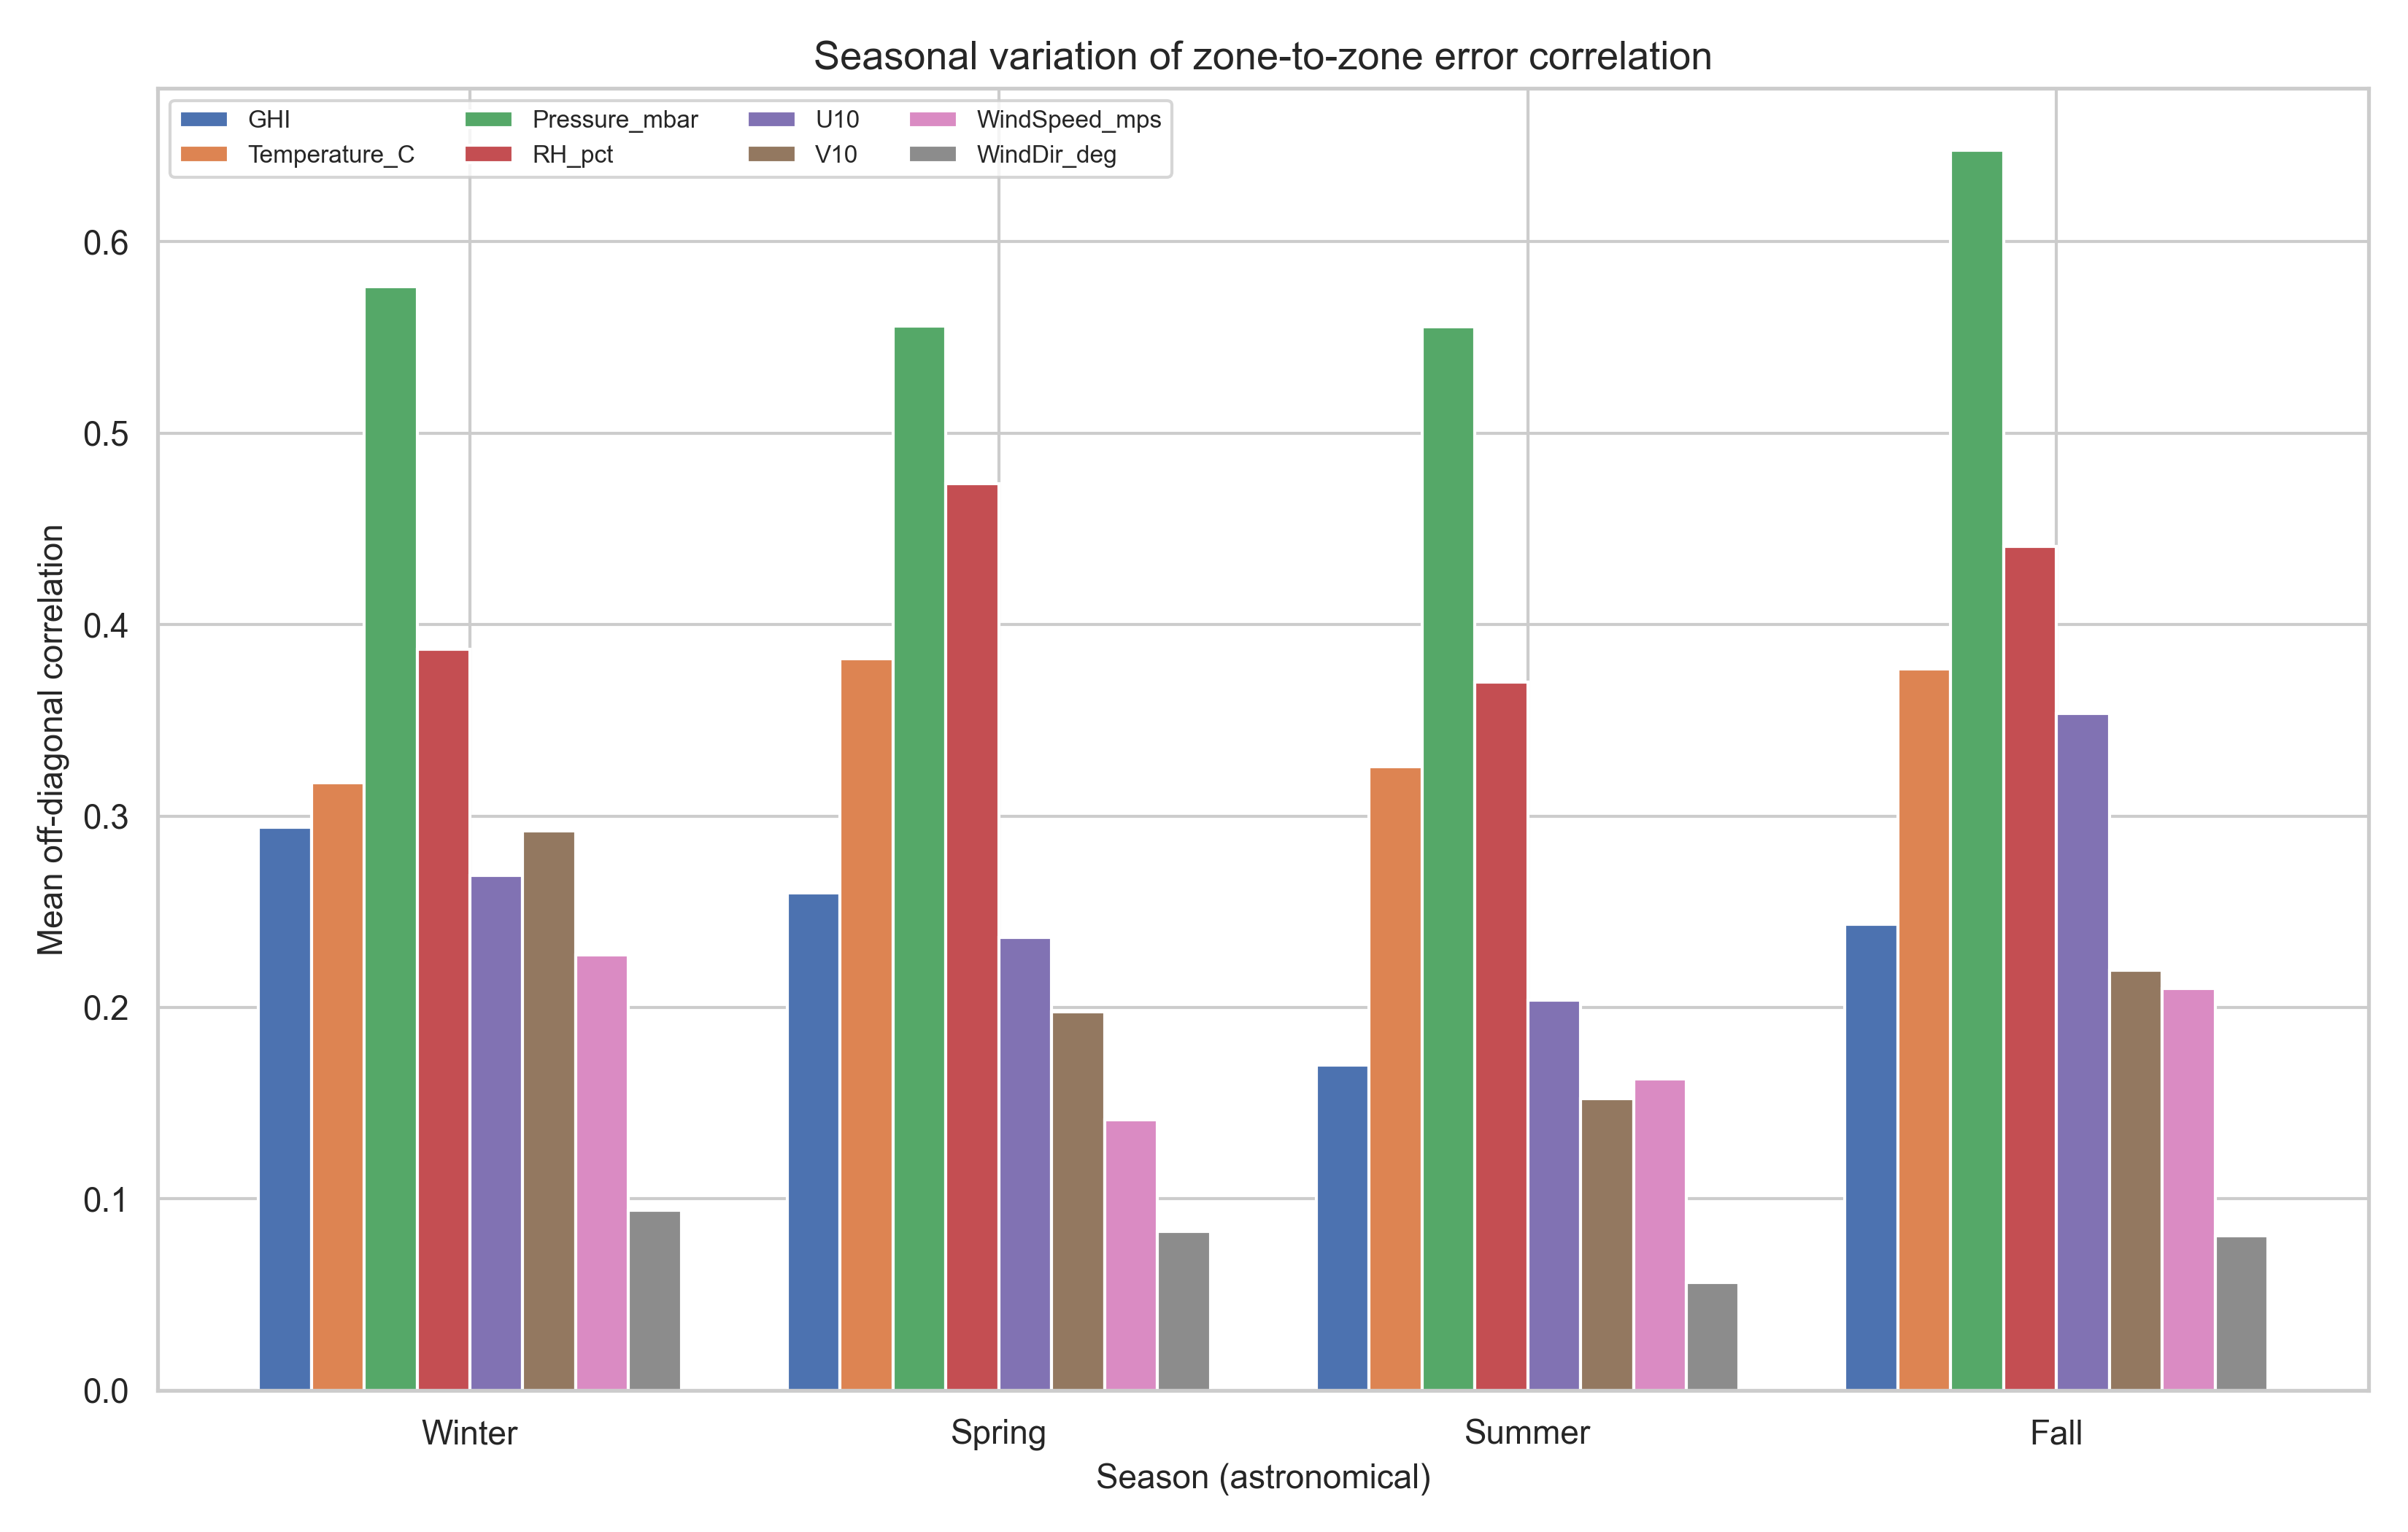
\includegraphics[width=\textwidth]{figures/Q9/seasonal_zone_correlation.png}
  \caption{Complete (all-variable) version of mean zone-to-zone correlation by season.}
  \label{fig:app_seasoncorr}
\end{figure}

\begin{figure}[H]
  \centering
  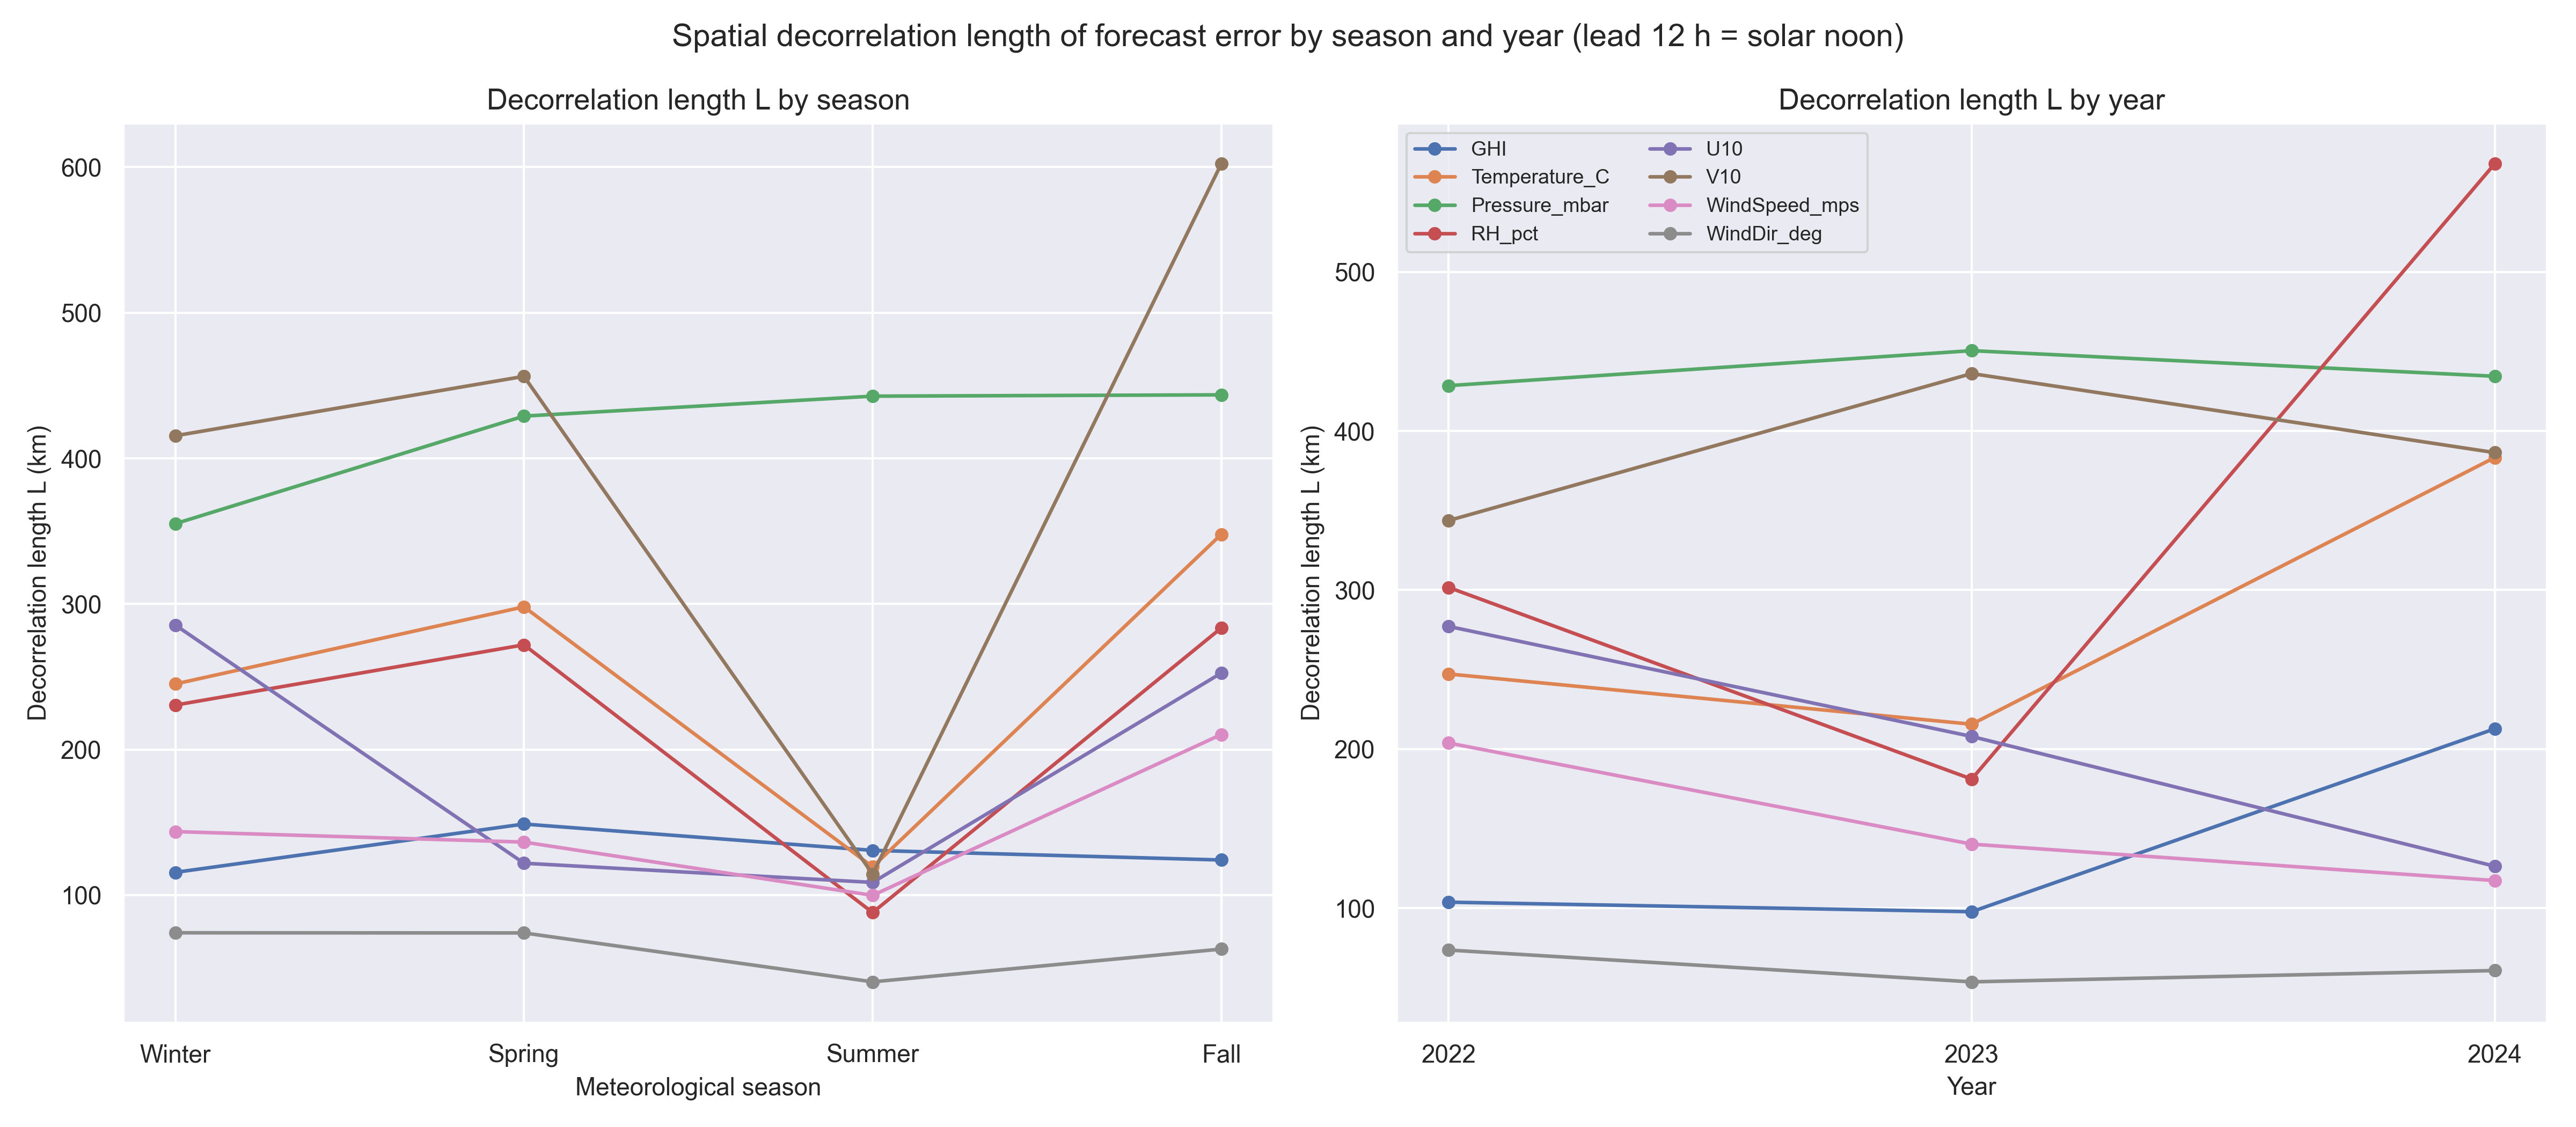
\includegraphics[width=\textwidth]{figures/Q9/decorrelation_length_by_season_year.png}
  \caption{Complete (all-variable) version of the fitted decorrelation length $L$ by season and year.}
  \label{fig:app_seasondecay}
\end{figure}

\begin{figure}[H]
  \centering
  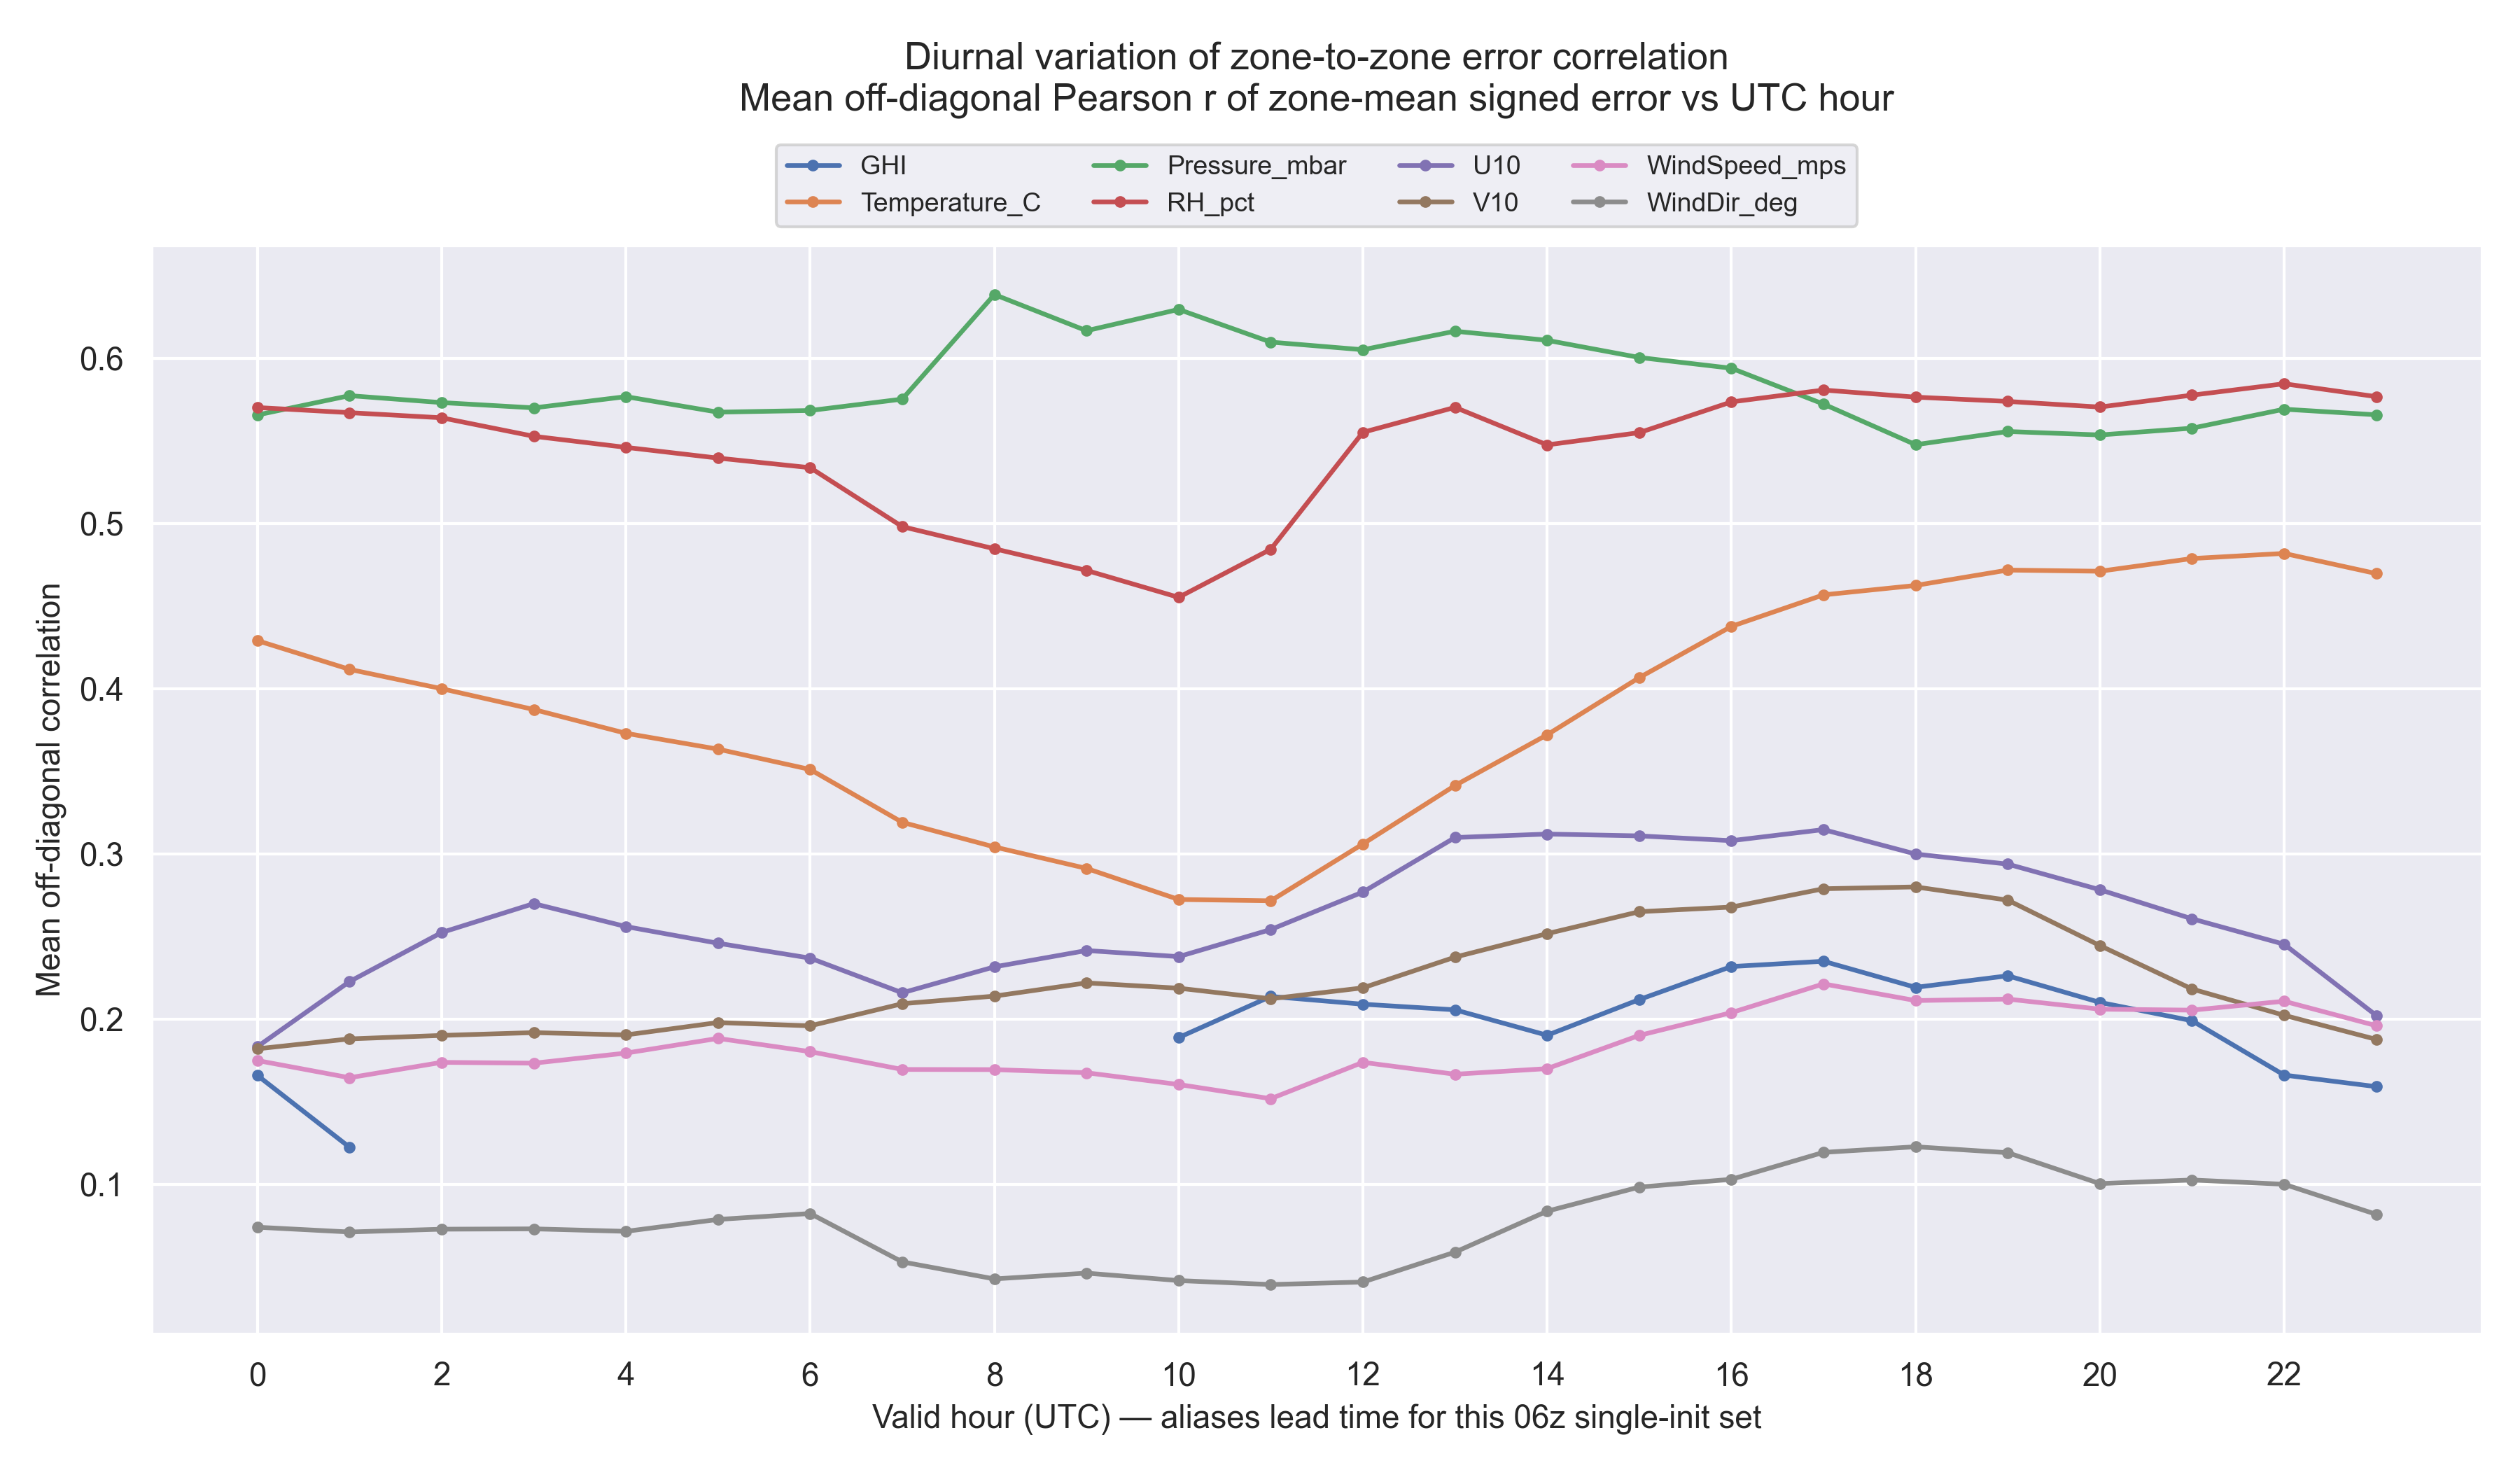
\includegraphics[width=\textwidth]{figures/Q9/diurnal_zone_correlation.png}
  \caption{Complete (all-variable) version of mean zone-to-zone correlation versus UTC hour.}
  \label{fig:app_diurnal}
\end{figure}

\begin{figure}[H]
  \centering
  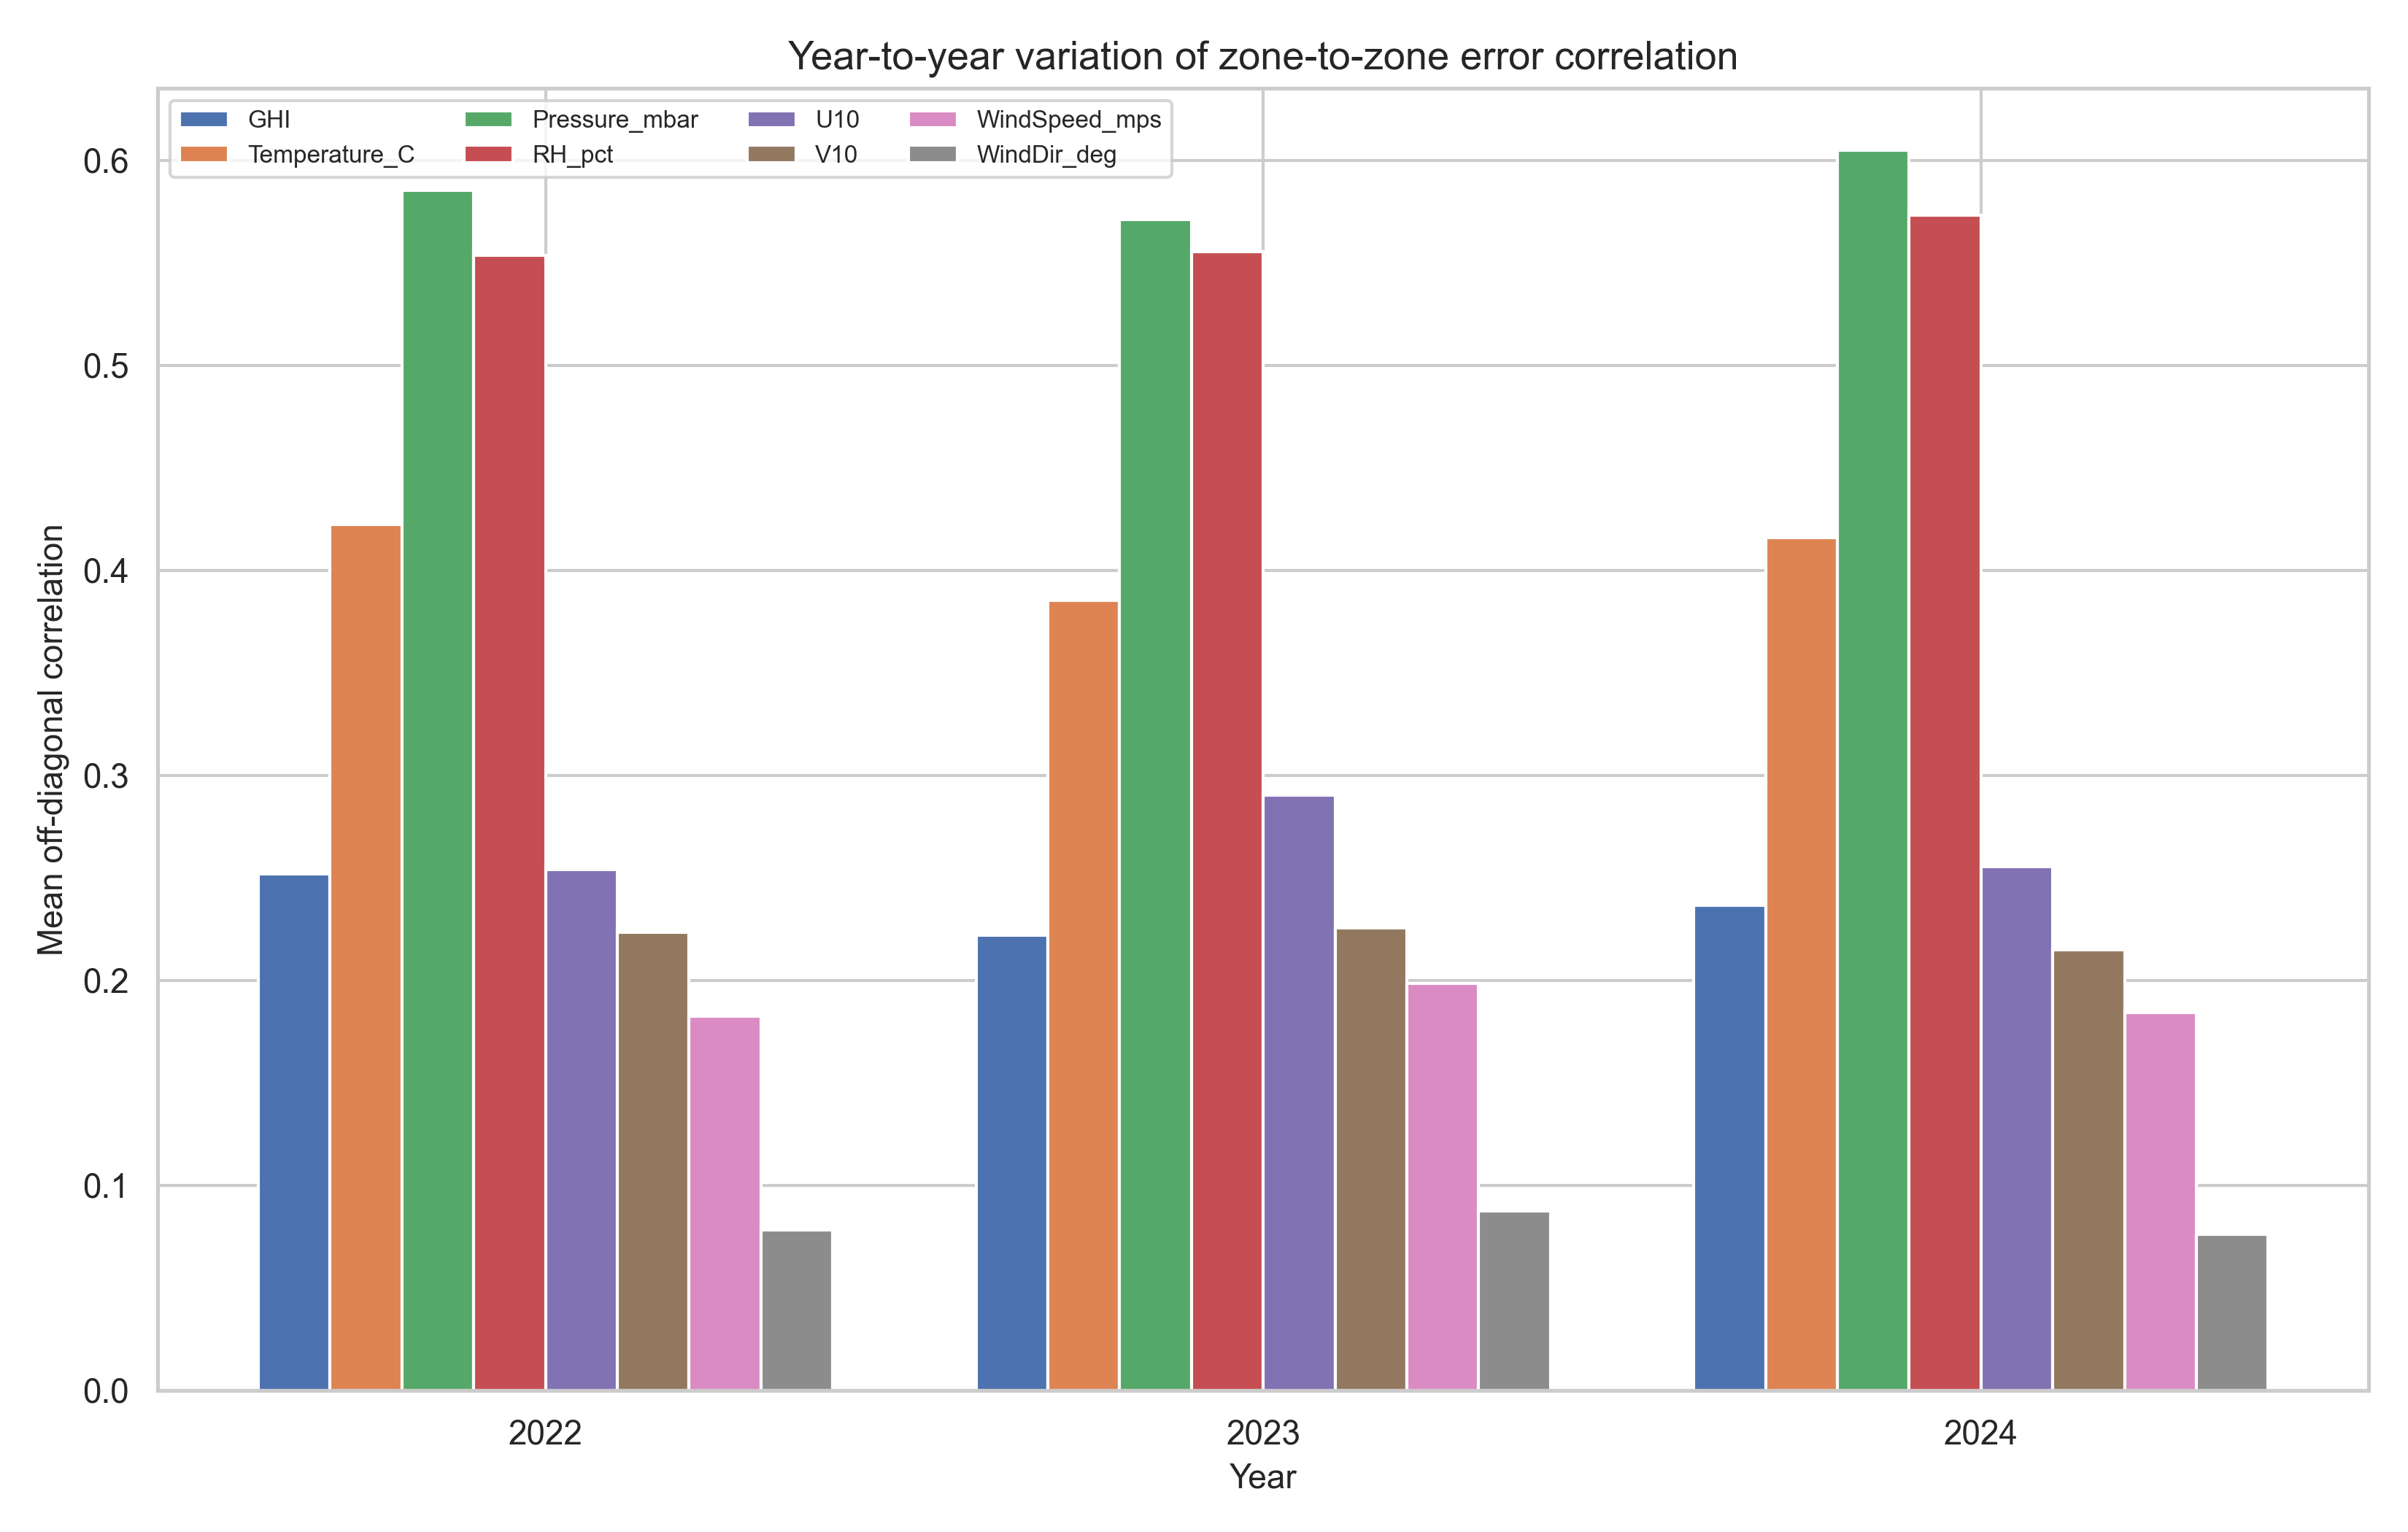
\includegraphics[width=\textwidth]{figures/Q9/yearly_zone_correlation.png}
  \caption{Complete (all-variable) version of year-to-year zone-to-zone forecast-error correlation.}
  \label{fig:app_yearcorr}
\end{figure}

\bibliography{references}

\end{document}
